\section{Frequency Response of Measured Data}

In this section the frequency response of the measured data will be analysed to examine if there is any correlation between the frequency responses and the performance of the loudspeaker. From previous section the presented data showed that minimal changes occurred between the datasets. Therefore the expectation is that the frequency response of the measurements will mostly likewise remain almost identical between the datasets. In \autoref{fig:freq_response1} the frequency response of the data measured from the accelerometers and microphone is shown for dataset 1.

\begin{figure}[H]
\centering
\begin{subfigure}[t]{0.37\textwidth}
	\tikzsetnextfilename{FFT_driver1}
	% This file was created by matlab2tikz.
%
%The latest updates can be retrieved from
%  http://www.mathworks.com/matlabcentral/fileexchange/22022-matlab2tikz-matlab2tikz
%where you can also make suggestions and rate matlab2tikz.
%
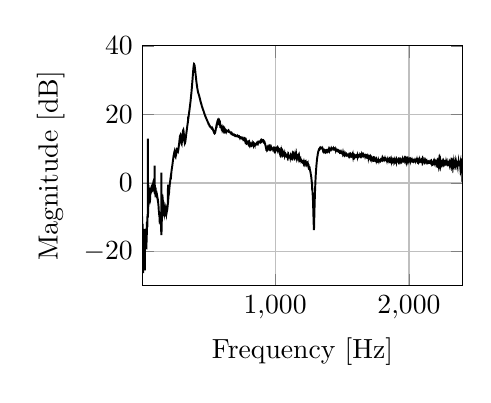
\begin{tikzpicture}

\begin{axis}[%
width=1.6in,
height=1.2in,
at={(1.011in,0.642in)},
scale only axis,
xmin=10,
xmax=2400,
xmajorgrids,
ymin=-30,
ymax=40,
ymajorgrids,
ylabel={Magnitude [dB]},
xlabel={Frequency [Hz]},
axis background/.style={fill=white}
]
\addplot [color=black,solid,line width=0.7pt,forget plot]
  table[row sep=crcr]{%
0	-19.3618707872866\\
0.666675926054529	-35.9021795514571\\
1.33335185210906	-20.4995835912269\\
2.00002777816359	-20.5444223053229\\
2.66670370421811	-9.88468154141047\\
3.33337963027264	-19.4430564977411\\
4.00005555632717	-19.9418145255131\\
4.6667314823817	-11.0447427372739\\
5.33340740843623	-16.0704359338039\\
6.00008333449076	-23.4702797128755\\
6.66675926054529	-15.6619663777543\\
7.33343518659981	-9.76687826406771\\
8.00011111265434	-19.81163092948\\
8.66678703870887	-17.2704521107206\\
9.3334629647634	-14.8299470465014\\
10.0001388908179	-20.9710252598229\\
10.6668148168725	-12.4462531922576\\
11.333490742927	-11.9282433167507\\
12.0001666689815	-20.3262262253202\\
12.666842595036	-19.7394025773231\\
13.3335185210906	-19.6473940807427\\
14.0001944471451	-26.2662831785163\\
14.6668703731996	-14.3734875190756\\
15.3335462992542	-15.6194052031707\\
16.0002222253087	-20.5496811876015\\
16.6668981513632	-22.2090559759572\\
17.3335740774177	-13.975664759218\\
18.0002500034723	-15.7219059175587\\
18.6669259295268	-18.9757168031201\\
19.3336018555813	-20.1126389030472\\
20.0002777816359	-20.0150779499674\\
20.6669537076904	-19.6692319589062\\
21.3336296337449	-20.2893657977048\\
22.0003055597994	-13.5845319182427\\
22.666981485854	-18.3651991731509\\
23.3336574119085	-18.3877906864951\\
24.000333337963	-23.6914867344971\\
24.6670092640176	-13.3952905774092\\
25.3336851900721	-14.8954912714511\\
26.0003611161266	-15.2317825176649\\
26.6670370421811	-14.3703796977619\\
27.3337129682357	-25.5165667215092\\
28.0003888942902	-13.7440540263342\\
28.6670648203447	-17.7645298009446\\
29.3337407463993	-14.7837657270799\\
30.0004166724538	-16.8735833588288\\
30.6670925985083	-17.2615490606666\\
31.3337685245628	-17.5057872025498\\
32.0004444506174	-16.2430944598921\\
32.6671203766719	-16.4407468828219\\
33.3337963027264	-17.3775675554526\\
34.000472228781	-18.1531539923639\\
34.6671481548355	-17.6636361452589\\
35.33382408089	-18.2668892181375\\
36.0005000069445	-19.3154779572481\\
36.6671759329991	-19.0730057493734\\
37.3338518590536	-17.4931961907791\\
38.0005277851081	-18.5459459068643\\
38.6672037111627	-18.5814342471402\\
39.3338796372172	-17.1293154163343\\
40.0005555632717	-17.3384234147972\\
40.6672314893262	-13.1347312756615\\
41.3339074153808	-15.5929452177734\\
42.0005833414353	-14.5776655625952\\
42.6672592674898	-11.4241252846142\\
43.3339351935444	-13.2368355069047\\
44.0006111195989	-12.2062110260313\\
44.6672870456534	-11.3220003063678\\
45.3339629717079	-12.9504502177195\\
46.0006388977625	-9.91595299096013\\
46.667314823817	-9.82517386458058\\
47.3339907498715	-10.1629820842313\\
48.0006666759261	-9.1029695267806\\
48.6673426019806	-9.80998740038481\\
49.3340185280351	-9.97000505908926\\
50.0006944540896	12.9240349727171\\
50.6673703801442	-7.21977883002444\\
51.3340463061987	-7.11446728172143\\
52.0007222322532	-8.97719564464933\\
52.6673981583078	-6.72063400953434\\
53.3340740843623	-6.3749580055128\\
54.0007500104168	-6.90631756701589\\
54.6674259364713	-6.30743722286645\\
55.3341018625259	-5.88202149675894\\
56.0007777885804	-5.61425232039832\\
56.6674537146349	-5.97918208872082\\
57.3341296406895	-5.37794492569941\\
58.000805566744	-4.89271215568237\\
58.6674814927985	-5.17338460687313\\
59.334157418853	-4.98600617637626\\
60.0008333449076	-4.85526946634448\\
60.6675092709621	-5.2761988980378\\
61.3341851970166	-3.78546843623239\\
62.0008611230712	-4.32617760644911\\
62.6675370491257	-4.54211696650046\\
63.3342129751802	-3.88517846686583\\
64.0008889012347	-4.02237599460151\\
64.6675648272893	-3.63286097665071\\
65.3342407533438	-3.87214301509673\\
66.0009166793983	-3.26523646091372\\
66.6675926054529	-3.72316484908041\\
67.3342685315074	-3.0928348687467\\
68.0009444575619	-3.24142211424055\\
68.6676203836164	-2.67465267727076\\
69.334296309671	-3.26876729871548\\
70.0009722357255	-2.63127500896192\\
70.66764816178	-2.51084178131243\\
71.3343240878346	-2.93847776060651\\
72.0010000138891	-2.31819970809246\\
72.6676759399436	-3.02553318854959\\
73.3343518659981	-2.43376505268678\\
74.0010277920527	-2.31815003861385\\
74.6677037181072	-2.31016640184259\\
75.3343796441617	-1.69491841027598\\
76.0010555702163	-2.22955738129066\\
76.6677314962708	-1.72027342301511\\
77.3344074223253	-1.6558429796661\\
78.0010833483798	-1.80714746843256\\
78.6677592744344	-1.81411401941666\\
79.3344352004889	-1.74565457439211\\
80.0011111265434	-1.52549072383373\\
80.667787052598	-1.58400244407407\\
81.3344629786525	-0.794793712460878\\
82.001138904707	-1.21720617302108\\
82.6678148307615	-1.32404377078639\\
83.3344907568161	-1.19859894415666\\
84.0011666828706	-1.54136539234771\\
84.6678426089251	-1.25417213799066\\
85.3345185349797	-1.59876693986671\\
86.0011944610342	-1.39127366917041\\
86.6678703870887	-1.3696455118177\\
87.3345463131432	-1.24349146129673\\
88.0012222391978	-1.32427084946929\\
88.6678981652523	-1.39971551325901\\
89.3345740913068	-1.17434411025682\\
90.0012500173614	-1.21083171739961\\
90.6679259434159	-1.2824931768613\\
91.3346018694704	-1.27007323884887\\
92.0012777955249	-0.966074720727181\\
92.6679537215795	-1.12262786063696\\
93.334629647634	-1.25910159242507\\
94.0013055736885	-1.00924206496683\\
94.667981499743	-1.19814649030848\\
95.3346574257976	-1.03793473306067\\
96.0013333518521	-0.985069630540586\\
96.6680092779066	-1.16576706251535\\
97.3346852039612	-1.13231955371233\\
98.0013611300157	-1.66764064822606\\
98.6680370560702	-1.28672331497108\\
99.3347129821248	-1.3445186725035\\
100.001388908179	5.03925813680822\\
100.668064834234	-1.24492409609696\\
101.334740760288	-1.84894853364229\\
102.001416686343	-1.5057135993022\\
102.668092612397	-1.62581664083084\\
103.334768538452	-1.96026321995936\\
104.001444464506	-1.80858605343605\\
104.668120390561	-1.87696249754052\\
105.334796316616	-1.77338599294492\\
106.00147224267	-1.96371233163815\\
106.668148168725	-2.43242825396346\\
107.334824094779	-1.99629794834388\\
108.001500020834	-2.07333842125666\\
108.668175946888	-2.04693878577049\\
109.334851872943	-2.7856581024142\\
110.001527798997	-2.28962283777454\\
110.668203725052	-2.82932525884246\\
111.334879651106	-2.74366176562584\\
112.001555577161	-2.77203713305229\\
112.668231503215	-2.81106168698214\\
113.33490742927	-3.29193002298192\\
114.001583355324	-2.85516807999158\\
114.668259281379	-3.25622357420913\\
115.334935207433	-2.87083513348013\\
116.001611133488	-3.20098014091963\\
116.668287059542	-3.13931560604944\\
117.334962985597	-3.21800656543537\\
118.001638911652	-3.60361366656882\\
118.668314837706	-4.17266244181744\\
119.334990763761	-3.97386570647672\\
120.001666689815	-4.10317537863612\\
120.66834261587	-4.55642386800676\\
121.335018541924	-4.25647477320912\\
122.001694467979	-4.39406873293558\\
122.668370394033	-4.51138804830031\\
123.335046320088	-4.98742159191303\\
124.001722246142	-5.14486191270147\\
124.668398172197	-4.75589633135072\\
125.335074098251	-5.43127085642699\\
126.001750024306	-5.64842885485132\\
126.66842595036	-5.30074903970846\\
127.335101876415	-6.04512020516773\\
128.001777802469	-6.29132072343327\\
128.668453728524	-6.50695924426763\\
129.335129654579	-6.82140368980889\\
130.001805580633	-7.47075787354341\\
130.668481506688	-7.55572763464663\\
131.335157432742	-8.21634295355302\\
132.001833358797	-8.32120016798544\\
132.668509284851	-8.37506524200766\\
133.335185210906	-8.9496274798399\\
134.00186113696	-9.27578626243634\\
134.668537063015	-8.80783005626224\\
135.335212989069	-9.2782531505472\\
136.001888915124	-9.64742916651176\\
136.668564841178	-9.46825003491031\\
137.335240767233	-10.4050921542696\\
138.001916693287	-11.3250511085103\\
138.668592619342	-11.5516815812687\\
139.335268545396	-11.1106617083089\\
140.001944471451	-11.7499094291161\\
140.668620397506	-10.1510233892866\\
141.33529632356	-11.157217772991\\
142.001972249615	-10.2106984049837\\
142.668648175669	-10.0510334437557\\
143.335324101724	-10.3268554510805\\
144.002000027778	-10.0355459586078\\
144.668675953833	-10.7763809377099\\
145.335351879887	-10.8587694825624\\
146.002027805942	-10.4799795322674\\
146.668703731996	-11.4493056473397\\
147.335379658051	-12.1437142770862\\
148.002055584105	-11.962164877165\\
148.66873151016	-13.5416518045528\\
149.335407436214	-14.1889118439315\\
150.002083362269	3.04128722772059\\
150.668759288323	-15.1869062815816\\
151.335435214378	-13.7380737628693\\
152.002111140433	-14.2196536995097\\
152.668787066487	-13.4046421317761\\
153.335462992542	-11.6471719266991\\
154.002138918596	-10.760690485525\\
154.668814844651	-8.41691304980566\\
155.335490770705	-7.38533557911436\\
156.00216669676	-6.02064320421254\\
156.668842622814	-5.46287813346268\\
157.335518548869	-5.04969251448635\\
158.002194474923	-4.50630124511883\\
158.668870400978	-4.43783654221954\\
159.335546327032	-4.88720353680776\\
160.002222253087	-5.06977429115913\\
160.668898179141	-5.19068972670615\\
161.335574105196	-5.64099493735669\\
162.00225003125	-5.56196878479219\\
162.668925957305	-6.01141409718634\\
163.335601883359	-6.75241892022081\\
164.002277809414	-6.538990401781\\
164.668953735469	-7.23450154339778\\
165.335629661523	-6.74809548714496\\
166.002305587578	-7.05029257720258\\
166.668981513632	-7.39507165753175\\
167.335657439687	-7.48702815002829\\
168.002333365741	-8.58992278330363\\
168.669009291796	-8.52914852452159\\
169.33568521785	-8.6499350226437\\
170.002361143905	-7.8212165466623\\
170.669037069959	-7.89120213363103\\
171.335712996014	-8.07367011944289\\
172.002388922068	-7.87410609432333\\
172.669064848123	-8.17219993186708\\
173.335740774177	-7.76390095527525\\
174.002416700232	-8.28752825751316\\
174.669092626286	-9.02660428520083\\
175.335768552341	-8.49123820860328\\
176.002444478396	-9.17787961327407\\
176.66912040445	-8.95991283252426\\
177.335796330505	-8.76127455026899\\
178.002472256559	-9.04680280690476\\
178.669148182614	-9.00947111443036\\
179.335824108668	-9.31841804953383\\
180.002500034723	-9.27939456248399\\
180.669175960777	-8.71202583157834\\
181.335851886832	-9.50555929637702\\
182.002527812886	-8.65467993330737\\
182.669203738941	-8.62737799434884\\
183.335879664995	-9.25840518347694\\
184.00255559105	-9.04713806452003\\
184.669231517104	-8.5769430502273\\
185.335907443159	-8.67916420279669\\
186.002583369213	-8.26380700268637\\
186.669259295268	-8.42703416133062\\
187.335935221323	-7.99077751566202\\
188.002611147377	-8.43371721076821\\
188.669287073432	-8.37654035264563\\
189.335962999486	-8.22655884060956\\
190.002638925541	-8.24542965380036\\
190.669314851595	-8.29516042022565\\
191.33599077765	-8.26974793241131\\
192.002666703704	-7.82383305400602\\
192.669342629759	-8.08518583158324\\
193.336018555813	-7.94370588210414\\
194.002694481868	-7.93350967469461\\
194.669370407922	-7.70096143221432\\
195.336046333977	-7.50573609828088\\
196.002722260031	-7.29973916755475\\
196.669398186086	-7.03754494912687\\
197.33607411214	-6.85627051694723\\
198.002750038195	-6.35118374603092\\
198.66942596425	-6.27329248670784\\
199.336101890304	-5.62064545943526\\
200.002777816359	-0.520653736743226\\
200.669453742413	-5.75155877791724\\
201.336129668468	-4.4796134774656\\
202.002805594522	-4.72430752959396\\
202.669481520577	-4.45546021526977\\
203.336157446631	-3.75557102781182\\
204.002833372686	-3.8760403407913\\
204.66950929874	-3.58209516706976\\
205.336185224795	-3.07413435211663\\
206.002861150849	-3.40025646658202\\
206.669537076904	-2.69080359845468\\
207.336213002958	-2.45267696602557\\
208.002888929013	-2.27657737542287\\
208.669564855067	-2.00718168263896\\
209.336240781122	-2.04701852008489\\
210.002916707176	-1.69324008482576\\
210.669592633231	-1.37541420512163\\
211.336268559286	-1.13288083349977\\
212.00294448534	-0.978882286512991\\
212.669620411395	-0.702656183358659\\
213.336296337449	-0.417395694808079\\
214.002972263504	-0.0938414326463799\\
214.669648189558	-0.0327216465792262\\
215.336324115613	0.148708855407083\\
216.003000041667	0.353599018349351\\
216.669675967722	0.640722273963735\\
217.336351893776	0.915434231330508\\
218.003027819831	1.08714478615943\\
218.669703745885	1.35820861389876\\
219.33637967194	1.39138473536075\\
220.003055597994	1.58445637848068\\
220.669731524049	1.92489091425733\\
221.336407450103	2.08392184258553\\
222.003083376158	2.29463658656951\\
222.669759302213	2.38872420024993\\
223.336435228267	2.32391680605784\\
224.003111154322	2.75108126293096\\
224.669787080376	2.85452164625662\\
225.336463006431	3.11943011750765\\
226.003138932485	3.25625659268346\\
226.66981485854	3.61479060230108\\
227.336490784594	3.78807072357767\\
228.003166710649	3.95529919063432\\
228.669842636703	4.16890859721735\\
229.336518562758	4.27608573371528\\
230.003194488812	4.45094403532182\\
230.669870414867	4.75972997884267\\
231.336546340921	4.81041865641967\\
232.003222266976	5.01992162693982\\
232.66989819303	5.1368566929275\\
233.336574119085	5.37977685110137\\
234.00325004514	5.57911241316725\\
234.669925971194	5.886281344509\\
235.336601897249	5.95716756450319\\
236.003277823303	6.24665076575757\\
236.669953749358	6.48035740261547\\
237.336629675412	6.59231804135953\\
238.003305601467	6.7595849546891\\
238.669981527521	6.96399230087505\\
239.336657453576	7.18840104598157\\
240.00333337963	7.34042905452338\\
240.670009305685	7.52067395403219\\
241.336685231739	7.78622676943283\\
242.003361157794	7.92212176337835\\
242.670037083848	8.02632475838035\\
243.336713009903	8.24755980034838\\
244.003388935957	8.31487755452782\\
244.670064862012	8.470129661696\\
245.336740788066	8.54651053668772\\
246.003416714121	8.66806739733013\\
246.670092640176	8.83423476835627\\
247.33676856623	8.86612833832024\\
248.003444492285	9.07134124641547\\
248.670120418339	9.19343952631\\
249.336796344394	9.23323500853091\\
250.003472270448	9.32917023555425\\
250.670148196503	9.22395032652007\\
251.336824122557	9.13451808256684\\
252.003500048612	9.08731067564757\\
252.670175974666	8.79771825972886\\
253.336851900721	8.47691499356256\\
254.003527826775	8.19265450674294\\
254.67020375283	8.11053299755807\\
255.336879678884	7.8776402441604\\
256.003555604939	7.79160855896555\\
256.670231530993	7.83822328837478\\
257.336907457048	7.76763923640498\\
258.003583383103	7.91120444175719\\
258.670259309157	7.91612951645949\\
259.336935235212	8.06824101762504\\
260.003611161266	8.07494836406927\\
260.670287087321	8.23213331881161\\
261.336963013375	8.35977759477462\\
262.00363893943	8.62660813340609\\
262.670314865484	8.76475356215733\\
263.336990791539	9.00975952747425\\
264.003666717593	9.2256387347976\\
264.670342643648	9.41713264155132\\
265.337018569702	9.59861537432747\\
266.003694495757	9.55659118309994\\
266.670370421811	9.69957805668921\\
267.337046347866	9.66825541135089\\
268.00372227392	9.79519246191875\\
268.670398199975	9.80416559193101\\
269.33707412603	9.82703383043057\\
270.003750052084	9.68425574584365\\
270.670425978139	9.55682305741921\\
271.337101904193	9.41527968725362\\
272.003777830248	9.35609483611069\\
272.670453756302	9.24650902633177\\
273.337129682357	9.21320342348463\\
274.003805608411	9.20658559249051\\
274.670481534466	9.1675925688572\\
275.33715746052	9.30950450253818\\
276.003833386575	9.40606610828403\\
276.670509312629	9.57354347722375\\
277.337185238684	9.65703031885105\\
278.003861164738	9.96843184510568\\
278.670537090793	10.109811346222\\
279.337213016847	10.2745766901816\\
280.003888942902	10.493837169901\\
280.670564868956	10.7057934412898\\
281.337240795011	10.9513089721492\\
282.003916721066	11.1196552776977\\
282.67059264712	11.3770962150196\\
283.337268573175	11.5223683607698\\
284.003944499229	11.7237586181509\\
284.670620425284	12.0345613251209\\
285.337296351338	12.2703988487711\\
286.003972277393	12.5279272205309\\
286.670648203447	12.7416227815932\\
287.337324129502	12.9073142387462\\
288.004000055556	13.1180975787029\\
288.670675981611	13.333831397237\\
289.337351907665	13.5670474406913\\
290.00402783372	13.6373832842423\\
290.670703759774	13.7336113664837\\
291.337379685829	13.8146802869948\\
292.004055611883	13.8867266611167\\
292.670731537938	13.9426041891924\\
293.337407463993	13.7950036884169\\
294.004083390047	13.7070665226796\\
294.670759316102	13.5445840514981\\
295.337435242156	13.308689775809\\
296.004111168211	13.0440508478036\\
296.670787094265	12.7680920257627\\
297.33746302032	12.4142136041678\\
298.004138946374	12.2450852754287\\
298.670814872429	11.9564549319363\\
299.337490798483	11.6258386404829\\
300.004166724538	12.2684439114719\\
300.670842650592	11.6229937666425\\
301.337518576647	11.4374183909306\\
302.004194502701	11.3813821254475\\
302.670870428756	11.6490669280708\\
303.33754635481	11.8056923728049\\
304.004222280865	11.9167095181664\\
304.67089820692	12.1013743018492\\
305.337574132974	12.4757414084964\\
306.004250059029	12.6877860532945\\
306.670925985083	12.9221839479462\\
307.337601911138	13.2515852007202\\
308.004277837192	13.6256753511003\\
308.670953763247	13.7629636930123\\
309.337629689301	14.0857124478674\\
310.004305615356	14.4385359063525\\
310.67098154141	14.6574312831774\\
311.337657467465	14.7989979451058\\
312.004333393519	15.1433103039367\\
312.671009319574	15.300451077485\\
313.337685245628	15.3596258012415\\
314.004361171683	15.4610068622099\\
314.671037097737	15.5093536938561\\
315.337713023792	15.3241037375253\\
316.004388949847	15.1987447944542\\
316.671064875901	15.0418771577208\\
317.337740801956	14.705894533561\\
318.00441672801	14.4189846794481\\
318.671092654065	14.071762199169\\
319.337768580119	13.6736985288621\\
320.004444506174	13.3741171124124\\
320.671120432228	13.1263467212002\\
321.337796358283	12.7215684804356\\
322.004472284337	12.4631415681196\\
322.671148210392	12.2463477055507\\
323.337824136446	12.0011302606234\\
324.004500062501	11.8984163784686\\
324.671175988555	11.7539313190426\\
325.33785191461	11.6269151414737\\
326.004527840664	11.7039112439033\\
326.671203766719	11.6990518883027\\
327.337879692774	11.6892884983601\\
328.004555618828	11.8944320306926\\
328.671231544883	11.9053719841116\\
329.337907470937	12.0472273530908\\
330.004583396992	12.2509789817655\\
330.671259323046	12.3680599176696\\
331.337935249101	12.638658943634\\
332.004611175155	12.7793608680765\\
332.67128710121	13.0093969748005\\
333.337963027264	13.2479431438629\\
334.004638953319	13.3902878141347\\
334.671314879373	13.6414326564039\\
335.337990805428	13.8752340445966\\
336.004666731482	14.072334978583\\
336.671342657537	14.3178892978025\\
337.338018583591	14.4548758441018\\
338.004694509646	14.7313876890009\\
338.671370435701	14.895318907374\\
339.338046361755	15.0835656030104\\
340.00472228781	15.3484762287606\\
340.671398213864	15.4749435079211\\
341.338074139919	15.7885587498514\\
342.004750065973	15.8653297787316\\
342.671425992028	16.1692239080047\\
343.338101918082	16.3364392416717\\
344.004777844137	16.5375356826601\\
344.671453770191	16.7465089878244\\
345.338129696246	16.8689924903991\\
346.0048056223	17.1428477313714\\
346.671481548355	17.2224447025625\\
347.338157474409	17.5285110516813\\
348.004833400464	17.6448279591173\\
348.671509326518	17.8805075734288\\
349.338185252573	18.0337037472689\\
350.004861178627	18.4750360674794\\
350.671537104682	18.4271588641798\\
351.338213030737	18.6396716938208\\
352.004888956791	18.817678443432\\
352.671564882846	19.0002002370105\\
353.3382408089	19.2145298232811\\
354.004916734955	19.3697422309362\\
354.671592661009	19.650137471914\\
355.338268587064	19.773616656178\\
356.004944513118	20.0281417507844\\
356.671620439173	20.1588654093105\\
357.338296365227	20.4255123616847\\
358.004972291282	20.5303176375592\\
358.671648217336	20.7990100777883\\
359.338324143391	20.9091847448413\\
360.005000069445	21.2009998211123\\
360.6716759955	21.3288520965485\\
361.338351921554	21.5974520900444\\
362.005027847609	21.7406101663951\\
362.671703773664	22.0036786609798\\
363.338379699718	22.1758939389062\\
364.005055625773	22.4092065617165\\
364.671731551827	22.6043360131825\\
365.338407477882	22.8145214531445\\
366.005083403936	23.0617249493562\\
366.671759329991	23.2383753963735\\
367.338435256045	23.5017511838225\\
368.0051111821	23.6618519776456\\
368.671787108154	23.977567524018\\
369.338463034209	24.1377164918625\\
370.005138960263	24.4722243451756\\
370.671814886318	24.6391151153694\\
371.338490812372	24.9651881333226\\
372.005166738427	25.1941275253484\\
372.671842664481	25.4573765925804\\
373.338518590536	25.7351898199429\\
374.005194516591	25.9486361440607\\
374.671870442645	26.2832248300519\\
375.3385463687	26.4693507438062\\
376.005222294754	26.8144423497695\\
376.671898220809	27.0407559976594\\
377.338574146863	27.3701293895772\\
378.005250072918	27.680314120169\\
378.671925998972	27.9504246390054\\
379.338601925027	28.3454701276926\\
380.005277851081	28.5897427933487\\
380.671953777136	28.9598274560529\\
381.33862970319	29.2536896482888\\
382.005305629245	29.5453436058301\\
382.671981555299	29.9355965603662\\
383.338657481354	30.1901741693537\\
384.005333407408	30.6024607334653\\
384.672009333463	30.9408032580226\\
385.338685259517	31.2464303425154\\
386.005361185572	31.6582574166453\\
386.672037111627	31.9166682784181\\
387.338713037681	32.274553603347\\
388.005388963736	32.6352470836804\\
388.67206488979	32.8866022402636\\
389.338740815845	33.274612379558\\
390.005416741899	33.5224629896123\\
390.672092667954	33.7326211728478\\
391.338768594008	34.0294594929755\\
392.005444520063	34.1528217813387\\
392.672120446117	34.3275564638173\\
393.338796372172	34.4921494668572\\
394.005472298226	34.4524799900155\\
394.672148224281	34.5059415132715\\
395.338824150335	34.5379844686153\\
396.00550007639	34.4529508200051\\
396.672176002444	34.4829120732413\\
397.338851928499	34.4345855545715\\
398.005527854554	34.27809377157\\
398.672203780608	34.2568437771917\\
399.338879706663	34.150150332169\\
400.005555632717	33.8825667999354\\
400.672231558772	33.7079545246617\\
401.338907484826	33.5456191717806\\
402.005583410881	33.2569646041632\\
402.672259336935	33.0118281021832\\
403.33893526299	32.8101399600196\\
404.005611189044	32.5135652481275\\
404.672287115099	32.2724666422037\\
405.338963041153	32.0603665146494\\
406.005638967208	31.7709155855659\\
406.672314893262	31.5044802920053\\
407.338990819317	31.3132797832042\\
408.005666745371	31.065515456776\\
408.672342671426	30.7580187562882\\
409.339018597481	30.5580858508745\\
410.005694523535	30.3814806356686\\
410.67237044959	30.0840019715765\\
411.339046375644	29.8351961702988\\
412.005722301699	29.7017199577745\\
412.672398227753	29.4682927059066\\
413.339074153808	29.194237507581\\
414.005750079862	29.0338915668757\\
414.672426005917	28.8537213867012\\
415.339101931971	28.6409556880654\\
416.005777858026	28.4209807945455\\
416.67245378408	28.2303070369924\\
417.339129710135	28.10569740321\\
418.005805636189	27.9013742615739\\
418.672481562244	27.6773246424915\\
419.339157488298	27.5411580665293\\
420.005833414353	27.4461017056009\\
420.672509340407	27.2479285245684\\
421.339185266462	27.0386024971026\\
422.005861192517	26.9571503298195\\
422.672537118571	26.8396501979411\\
423.339213044626	26.7515608658471\\
424.00588897068	26.5615335036433\\
424.672564896735	26.4335183800764\\
425.339240822789	26.3898871635666\\
426.005916748844	26.3303199681989\\
426.672592674898	26.1673378111597\\
427.339268600953	26.0862711715932\\
428.005944527007	25.9948121779699\\
428.672620453062	25.9758807816233\\
429.339296379116	25.8911701560308\\
430.005972305171	25.7621120146669\\
430.672648231225	25.6623947562977\\
431.33932415728	25.5856764220714\\
432.006000083334	25.5443756100151\\
432.672676009389	25.4873050488812\\
433.339351935444	25.3240776275726\\
434.006027861498	25.2329882518413\\
434.672703787553	25.0844787960022\\
435.339379713607	25.073088832736\\
436.006055639662	24.9697441411312\\
436.672731565716	24.8721485403557\\
437.339407491771	24.7170291418084\\
438.006083417825	24.5580523600165\\
438.67275934388	24.4958749979621\\
439.339435269934	24.3796001834163\\
440.006111195989	24.3511004999882\\
440.672787122043	24.1954836461562\\
441.339463048098	24.0752971763901\\
442.006138974152	23.9383321411095\\
442.672814900207	23.8441399968708\\
443.339490826261	23.7755733812962\\
444.006166752316	23.7002205221968\\
444.672842678371	23.6007989924081\\
445.339518604425	23.5099756219178\\
446.00619453048	23.3793801644176\\
446.672870456534	23.2498904206607\\
447.339546382589	23.1675170539806\\
448.006222308643	23.0814009437549\\
448.672898234698	23.0116942793781\\
449.339574160752	22.964840851347\\
450.006250086807	22.9458704611028\\
450.672926012861	22.7783538254155\\
451.339601938916	22.6382110135418\\
452.00627786497	22.5476970468293\\
452.672953791025	22.4317637900438\\
453.339629717079	22.3681217755119\\
454.006305643134	22.2761764703997\\
454.672981569188	22.2294736097782\\
455.339657495243	22.1449451202068\\
456.006333421298	22.1160098296591\\
456.673009347352	22.0060886937568\\
457.339685273407	21.9304768469233\\
458.006361199461	21.8244093856888\\
458.673037125516	21.7316223491682\\
459.33971305157	21.6257007503832\\
460.006388977625	21.5309560014764\\
460.673064903679	21.4782096457126\\
461.339740829734	21.4014578573023\\
462.006416755788	21.3592599180213\\
462.673092681843	21.256840338377\\
463.339768607897	21.2065775637823\\
464.006444533952	21.1350130881169\\
464.673120460006	21.0839212617895\\
465.339796386061	21.0055807317284\\
466.006472312115	20.9206656945536\\
466.67314823817	20.8391310697489\\
467.339824164225	20.7488575893734\\
468.006500090279	20.6839066870886\\
468.673176016334	20.6176278655441\\
469.339851942388	20.515563407399\\
470.006527868443	20.4489964588962\\
470.673203794497	20.3415372715676\\
471.339879720552	20.2434423446577\\
472.006555646606	20.2238547972236\\
472.673231572661	20.1500104700638\\
473.339907498715	20.0641149313031\\
474.00658342477	20.0155520841237\\
474.673259350824	19.8984088787438\\
475.339935276879	19.8167830452497\\
476.006611202933	19.7829865189436\\
476.673287128988	19.6697896991569\\
477.339963055042	19.5995051883076\\
478.006638981097	19.5952348274665\\
478.673314907152	19.5014798057631\\
479.339990833206	19.4176958625874\\
480.006666759261	19.3725855091289\\
480.673342685315	19.2757692541619\\
481.34001861137	19.2196493243922\\
482.006694537424	19.2042050143783\\
482.673370463479	19.0951235276728\\
483.340046389533	19.0102230895272\\
484.006722315588	18.9773397078674\\
484.673398241642	18.9312526849428\\
485.340074167697	18.8557475227714\\
486.006750093751	18.7949903251266\\
486.673426019806	18.7466929988789\\
487.34010194586	18.690511732119\\
488.006777871915	18.6189838500254\\
488.673453797969	18.5860954078857\\
489.340129724024	18.5331296321922\\
490.006805650078	18.4579266990112\\
490.673481576133	18.372315235375\\
491.340157502188	18.3319678573866\\
492.006833428242	18.2823146786698\\
492.673509354297	18.1736580621393\\
493.340185280351	18.1154465819649\\
494.006861206406	18.0874254414673\\
494.67353713246	17.9971101242718\\
495.340213058515	17.9153642911631\\
496.006888984569	17.8558607499057\\
496.673564910624	17.8272089195585\\
497.340240836678	17.7689684682805\\
498.006916762733	17.7240616823976\\
498.673592688787	17.6788090881146\\
499.340268614842	17.6161004207237\\
500.006944540896	17.5310425513652\\
500.673620466951	17.4425271469796\\
501.340296393005	17.3418460395877\\
502.00697231906	17.2758221677175\\
502.673648245115	17.267028255022\\
503.340324171169	17.2781276668744\\
504.007000097224	17.210917417503\\
504.673676023278	17.1200646646595\\
505.340351949333	17.1059976868596\\
506.007027875387	17.1007664238695\\
506.673703801442	17.0331785872377\\
507.340379727496	16.9913466987233\\
508.007055653551	16.8890069270035\\
508.673731579605	16.7891066779324\\
509.34040750566	16.7300467123014\\
510.007083431714	16.7381196955819\\
510.673759357769	16.7328369246324\\
511.340435283823	16.7169103707291\\
512.007111209878	16.6382801236244\\
512.673787135932	16.547096015275\\
513.340463061987	16.4854386771388\\
514.007138988041	16.4542937923094\\
514.673814914096	16.4454673311036\\
515.340490840151	16.4489332837606\\
516.007166766205	16.4147961994688\\
516.67384269226	16.3885516307465\\
517.340518618314	16.2706279815487\\
518.007194544369	16.2591221149596\\
518.673870470423	16.233324992577\\
519.340546396478	16.244104383152\\
520.007222322532	16.2195029701752\\
520.673898248587	16.1556079743307\\
521.340574174641	16.1440169406125\\
522.007250100696	16.1674559478337\\
522.67392602675	16.1547922202727\\
523.340601952805	16.1554122758746\\
524.007277878859	16.152751152871\\
524.673953804914	16.1225027133183\\
525.340629730968	16.0499008571852\\
526.007305657023	16.0795852066358\\
526.673981583078	16.1017003009515\\
527.340657509132	16.0856263004078\\
528.007333435187	16.0056037949166\\
528.674009361241	15.9978384794813\\
529.340685287296	15.9499654219996\\
530.00736121335	16.003658067844\\
530.674037139405	15.9471291338518\\
531.340713065459	15.8773895206512\\
532.007388991514	15.8553531599656\\
532.674064917568	15.8745775444435\\
533.340740843623	15.8172777924018\\
534.007416769677	15.751167853204\\
534.674092695732	15.647045896088\\
535.340768621786	15.6247740794223\\
536.007444547841	15.582567223678\\
536.674120473896	15.4662287045036\\
537.34079639995	15.3955257377633\\
538.007472326005	15.3540519147725\\
538.674148252059	15.3184859454046\\
539.340824178114	15.2142494108425\\
540.007500104168	15.0955185860154\\
540.674176030223	15.062525615901\\
541.340851956277	15.0007524619735\\
542.007527882332	14.9025895827768\\
542.674203808386	14.8018046876672\\
543.340879734441	14.7850196988538\\
544.007555660495	14.7340519595461\\
544.67423158655	14.6269471808843\\
545.340907512604	14.6217859780869\\
546.007583438659	14.5934141185214\\
546.674259364713	14.534385789673\\
547.340935290768	14.4938739308286\\
548.007611216823	14.5311076929047\\
548.674287142877	14.5753219172441\\
549.340963068932	14.4832816844596\\
550.007638994986	14.5024924292087\\
550.674314921041	14.6453692764469\\
551.340990847095	14.6303311481102\\
552.00766677315	14.7006516644172\\
552.674342699204	14.8781835538091\\
553.341018625259	14.8764908876774\\
554.007694551313	14.995040459506\\
554.674370477368	15.1276311512138\\
555.341046403422	15.2651930513634\\
556.007722329477	15.4016446287971\\
556.674398255531	15.5902671350371\\
557.341074181586	15.7385518181621\\
558.00775010764	15.8431428971125\\
558.674426033695	16.0986336876973\\
559.341101959749	16.2007778182753\\
560.007777885804	16.2836797149855\\
560.674453811858	16.5437508861976\\
561.341129737913	16.5899679771811\\
562.007805663968	16.7156325267429\\
562.674481590022	16.9194361753216\\
563.341157516077	16.9085567183153\\
564.007833442131	17.1211072544243\\
564.674509368186	17.1512557343425\\
565.34118529424	17.0857459059384\\
566.007861220295	17.3069040450994\\
566.674537146349	17.4528274790765\\
567.341213072404	17.5256146547363\\
568.007888998458	17.6918720512982\\
568.674564924513	17.6703158465671\\
569.341240850567	17.7938311019778\\
570.007916776622	17.8906645467607\\
570.674592702676	17.826349172351\\
571.341268628731	17.9664138185063\\
572.007944554785	17.966508251008\\
572.67462048084	17.9574442607058\\
573.341296406895	18.0296151345562\\
574.007972332949	17.999888482376\\
574.674648259004	18.106721858489\\
575.341324185058	18.059163234698\\
576.008000111113	18.0474279390616\\
576.674676037167	18.0904361152733\\
577.341351963222	17.9682624220956\\
578.008027889276	18.0611991994242\\
578.674703815331	17.9689211591393\\
579.341379741385	17.9958547488359\\
580.00805566744	17.9259833215245\\
580.674731593494	17.8496803933777\\
581.341407519549	17.9143362018226\\
582.008083445603	17.7492996791415\\
582.674759371658	17.8030287711394\\
583.341435297712	17.6432104530114\\
584.008111223767	17.6781893434403\\
584.674787149822	17.5529599100494\\
585.341463075876	17.5158046063981\\
586.008139001931	17.5143171799659\\
586.674814927985	17.358332057589\\
587.34149085404	17.3509933314181\\
588.008166780094	17.1707471744715\\
588.674842706149	17.2378131402912\\
589.341518632203	17.0291383177995\\
590.008194558258	17.0820169695886\\
590.674870484312	16.8696166053489\\
591.341546410367	16.8689438635772\\
592.008222336421	16.6909351796721\\
592.674898262476	16.7283398771291\\
593.34157418853	16.6093793369855\\
594.008250114585	16.5725131254014\\
594.674926040639	16.489629826362\\
595.341601966694	16.4613662983083\\
596.008277892749	16.3360261545365\\
596.674953818803	16.2886794174475\\
597.341629744858	16.2324550134901\\
598.008305670912	16.1744263898047\\
598.674981596967	16.079717588956\\
599.341657523021	16.1259435635265\\
600.008333449076	15.9767148955137\\
600.67500937513	16.0139479376889\\
601.341685301185	15.9254718077809\\
602.008361227239	15.9435933343133\\
602.675037153294	15.8624794178313\\
603.341713079348	15.906156928152\\
604.008389005403	15.7747610080793\\
604.675064931457	15.8888550080739\\
605.341740857512	15.761247222628\\
606.008416783566	15.8165923481738\\
606.675092709621	15.7496528386067\\
607.341768635676	15.7508714646688\\
608.00844456173	15.6857656912273\\
608.675120487785	15.7167625244519\\
609.341796413839	15.6995488269068\\
610.008472339894	15.6424265324421\\
610.675148265948	15.6646889860933\\
611.341824192003	15.5981063503046\\
612.008500118057	15.6954236013886\\
612.675176044112	15.5575633767151\\
613.341851970166	15.6133037649105\\
614.008527896221	15.5459740740405\\
614.675203822275	15.5504160664722\\
615.34187974833	15.5655742560186\\
616.008555674384	15.4618995923198\\
616.675231600439	15.5687384925729\\
617.341907526493	15.4737390839156\\
618.008583452548	15.5199889963706\\
618.675259378603	15.4965481480473\\
619.341935304657	15.4710211904958\\
620.008611230711	15.50636608978\\
620.675287156766	15.3896184829142\\
621.341963082821	15.4296222622508\\
622.008639008875	15.406192517108\\
622.67531493493	15.3170342522488\\
623.341990860984	15.4162122020578\\
624.008666787039	15.2830087759572\\
624.675342713093	15.2979620938838\\
625.342018639148	15.3215521484245\\
626.008694565202	15.2020027546952\\
626.675370491257	15.2603739246503\\
627.342046417311	15.1819334534858\\
628.008722343366	15.1829092050369\\
628.67539826942	15.2310981588317\\
629.342074195475	15.1424132219261\\
630.008750121529	15.1299404551401\\
630.675426047584	15.1044124484591\\
631.342101973638	15.0384233724096\\
632.008777899693	15.0628907154921\\
632.675453825748	15.0643895175643\\
633.342129751802	14.991755602926\\
634.008805677857	15.0289376836571\\
634.675481603911	14.9567612139926\\
635.342157529966	15.0404620075365\\
636.00883345602	15.0039848712989\\
636.675509382075	15.0038177581841\\
637.342185308129	15.0024032748583\\
638.008861234184	15.05293545392\\
638.675537160238	14.9832680858656\\
639.342213086293	14.9901300836212\\
640.008889012347	15.0591159996423\\
640.675564938402	15.044859025629\\
641.342240864456	15.083351266305\\
642.008916790511	15.1263758033044\\
642.675592716565	15.1028332768199\\
643.34226864262	15.1055323300386\\
644.008944568675	15.1209244741918\\
644.675620494729	15.1658218038784\\
645.342296420784	15.1515474544963\\
646.008972346838	15.1795048076326\\
646.675648272893	15.1905055639529\\
647.342324198947	15.1396839278998\\
648.009000125002	15.1375807670928\\
648.675676051056	15.178874057423\\
649.342351977111	15.2010996414745\\
650.009027903165	15.1899210122617\\
650.67570382922	15.1515109708583\\
651.342379755274	15.195063979341\\
652.009055681329	15.1197695293232\\
652.675731607383	15.1109590932212\\
653.342407533438	15.1430706776879\\
654.009083459492	15.060146027094\\
654.675759385547	15.0397822060428\\
655.342435311602	15.0136621212574\\
656.009111237656	15.0264153167971\\
656.675787163711	15.0010667411867\\
657.342463089765	14.9359942129756\\
658.00913901582	14.9456725312995\\
658.675814941874	14.937564205371\\
659.342490867929	14.9330347757354\\
660.009166793983	14.8476593767594\\
660.675842720038	14.8298010178927\\
661.342518646092	14.8521411911059\\
662.009194572147	14.8138021405902\\
662.675870498201	14.7799592033147\\
663.342546424256	14.7602882786645\\
664.00922235031	14.7843995700771\\
664.675898276365	14.7613031185636\\
665.342574202419	14.6997739103442\\
666.009250128474	14.647849207414\\
666.675926054529	14.6741076767612\\
667.342601980583	14.658983418656\\
668.009277906638	14.6340029278413\\
668.675953832692	14.5802675738556\\
669.342629758747	14.5500436678723\\
670.009305684801	14.526178486487\\
670.675981610856	14.5394770773497\\
671.34265753691	14.5219385320991\\
672.009333462965	14.4986132756945\\
672.676009389019	14.4352178124029\\
673.342685315074	14.4485954476707\\
674.009361241128	14.4878402138349\\
674.676037167183	14.4013804107998\\
675.342713093237	14.4192010349633\\
676.009389019292	14.3625027237386\\
676.676064945346	14.343631158623\\
677.342740871401	14.3402153760337\\
678.009416797456	14.3082554796504\\
678.67609272351	14.3442732888289\\
679.342768649565	14.2861876061887\\
680.009444575619	14.2689792423788\\
680.676120501674	14.2123174718637\\
681.342796427728	14.2336900519799\\
682.009472353783	14.238650398911\\
682.676148279837	14.2133455917976\\
683.342824205892	14.2244965388138\\
684.009500131946	14.1629816041953\\
684.676176058001	14.1302589440397\\
685.342851984055	14.1066697218618\\
686.00952791011	14.1357085205693\\
686.676203836164	14.102929134461\\
687.342879762219	14.1359172429107\\
688.009555688273	14.1156655571112\\
688.676231614328	14.0913762570809\\
689.342907540382	14.029543568363\\
690.009583466437	14.0179752259669\\
690.676259392492	14.0016672403027\\
691.342935318546	14.0045088610928\\
692.009611244601	14.0253395338315\\
692.676287170655	13.9844126382275\\
693.34296309671	13.9683046235232\\
694.009639022764	13.985898212397\\
694.676314948819	13.9584388282645\\
695.342990874873	13.9291291440968\\
696.009666800928	13.958451935271\\
696.676342726982	13.921909930188\\
697.343018653037	13.8815257231815\\
698.009694579091	13.8551671378551\\
698.676370505146	13.8318432190888\\
699.3430464312	13.8788000375133\\
700.009722357255	13.8386692913296\\
700.676398283309	13.8642243706605\\
701.343074209364	13.8919960314968\\
702.009750135419	13.8970949708776\\
702.676426061473	13.908649011525\\
703.343101987528	13.867472690205\\
704.009777913582	13.8472921888497\\
704.676453839637	13.8153997187105\\
705.343129765691	13.8194229330283\\
706.009805691746	13.8193839467886\\
706.6764816178	13.7576744413756\\
707.343157543855	13.7281335630431\\
708.009833469909	13.7581090389923\\
708.676509395964	13.7336444513536\\
709.343185322018	13.7368958052653\\
710.009861248073	13.7404630204994\\
710.676537174127	13.720487741455\\
711.343213100182	13.7038925605696\\
712.009889026236	13.7181577154569\\
712.676564952291	13.7335300093784\\
713.343240878346	13.7577661581475\\
714.0099168044	13.7601406807116\\
714.676592730455	13.7366848146595\\
715.343268656509	13.7165988254693\\
716.009944582564	13.7062605715623\\
716.676620508618	13.7301886799278\\
717.343296434673	13.6846240935792\\
718.009972360727	13.6841924107272\\
718.676648286782	13.7175729878836\\
719.343324212836	13.6415952930352\\
720.010000138891	13.6483893505625\\
720.676676064945	13.6483449021777\\
721.343351991	13.6215366069217\\
722.010027917054	13.6291236851842\\
722.676703843109	13.654633097726\\
723.343379769163	13.6096098008079\\
724.010055695218	13.5721151672515\\
724.676731621273	13.5858637068171\\
725.343407547327	13.5478677057616\\
726.010083473382	13.5696625277931\\
726.676759399436	13.5325465036717\\
727.343435325491	13.5615185372619\\
728.010111251545	13.5466849020637\\
728.6767871776	13.5685429756374\\
729.343463103654	13.5786128955822\\
730.010139029709	13.5405076255293\\
730.676814955763	13.5675248733976\\
731.343490881818	13.5860519296907\\
732.010166807872	13.5335257802545\\
732.676842733927	13.4821114190032\\
733.343518659981	13.4454154861402\\
734.010194586036	13.3868015219426\\
734.67687051209	13.3644298004664\\
735.343546438145	13.3412333772738\\
736.0102223642	13.3290768855355\\
736.676898290254	13.259861063814\\
737.343574216309	13.3489657320765\\
738.010250142363	13.3250303096578\\
738.676926068418	13.346910397895\\
739.343601994472	13.3460464182725\\
740.010277920527	13.3451647607941\\
740.676953846581	13.2743684872826\\
741.343629772636	13.2017987113616\\
742.01030569869	13.1174332027916\\
742.676981624745	13.1181665794177\\
743.343657550799	13.1619966972896\\
744.010333476854	13.2088612653572\\
744.677009402908	13.1827927301895\\
745.343685328963	13.1677012226232\\
746.010361255017	13.1204129038755\\
746.677037181072	13.1066997017076\\
747.343713107127	13.0779342325855\\
748.010389033181	13.027765696596\\
748.677064959236	13.0200117247697\\
749.34374088529	13.0515695854367\\
750.010416811345	13.1011932069225\\
750.677092737399	13.0765327786098\\
751.343768663454	13.062743954509\\
752.010444589508	13.0234907363263\\
752.677120515563	12.915229297473\\
753.343796441617	12.9078552517946\\
754.010472367672	12.9750077786914\\
754.677148293726	13.0475255385649\\
755.343824219781	13.0111054356309\\
756.010500145835	12.8967808868795\\
756.67717607189	12.8722488677805\\
757.343851997944	12.8999443995808\\
758.010527923999	12.9678212910269\\
758.677203850054	12.9341222028267\\
759.343879776108	12.8952145884744\\
760.010555702162	12.8800271318284\\
760.677231628217	12.8433816295036\\
761.343907554272	12.7688938392208\\
762.010583480326	12.817057567726\\
762.677259406381	12.8813228497882\\
763.343935332435	12.8321431531282\\
764.01061125849	12.7035393455459\\
764.677287184544	12.6933336234692\\
765.343963110599	12.7937769525569\\
766.010639036653	12.7880499823581\\
766.677314962708	12.6795334340502\\
767.343990888762	12.6250611543289\\
768.010666814817	12.6365425805558\\
768.677342740871	12.6812556725178\\
769.344018666926	12.5955510900948\\
770.01069459298	12.6065046038311\\
770.677370519035	12.5694564576013\\
771.344046445089	12.5221791126319\\
772.010722371144	12.6278537968144\\
772.677398297199	12.5634413797002\\
773.344074223253	12.4161992845673\\
774.010750149308	12.4064247671703\\
774.677426075362	12.4937433663734\\
775.344102001417	12.4249752297075\\
776.010777927471	12.3158613673551\\
776.677453853526	12.3873756957646\\
777.34412977958	12.3607734372351\\
778.010805705635	12.2584696901824\\
778.677481631689	12.2077551447013\\
779.344157557744	12.2149410397764\\
780.010833483798	12.3003354874215\\
780.677509409853	12.1666724230239\\
781.344185335907	12.0790013107712\\
782.010861261962	12.191737184683\\
782.677537188016	12.1506284083845\\
783.344213114071	12.0152042706424\\
784.010889040126	11.9893037055737\\
784.67756496618	12.0833387315967\\
785.344240892235	11.9683714140871\\
786.010916818289	12.0103327972703\\
786.677592744344	11.9210824571876\\
787.344268670398	11.9341252303138\\
788.010944596453	11.8328241826162\\
788.677620522507	11.8792972850034\\
789.344296448562	11.891475737927\\
790.010972374616	11.7847911471909\\
790.677648300671	11.830650650303\\
791.344324226725	11.7559509887335\\
792.01100015278	11.676384975047\\
792.677676078834	11.7022927716067\\
793.344352004889	11.7314003882175\\
794.011027930943	11.6684009756146\\
794.677703856998	11.6887078884818\\
795.344379783053	11.6836806310548\\
796.011055709107	11.6630738747621\\
796.677731635162	11.6071883735226\\
797.344407561216	11.5742879767542\\
798.011083487271	11.5998810229313\\
798.677759413325	11.5880173662061\\
799.34443533938	11.5110194558863\\
800.011111265434	11.58222798717\\
800.677787191489	11.4850438601538\\
801.344463117543	11.4638428039074\\
802.011139043598	11.4623373172617\\
802.677814969652	11.5284422184286\\
803.344490895707	11.398582630429\\
804.011166821761	11.4551498268127\\
804.677842747816	11.3962076334421\\
805.34451867387	11.408894533225\\
806.011194599925	11.3676521003675\\
806.67787052598	11.3761691648252\\
807.344546452034	11.3815522808551\\
808.011222378089	11.352525664825\\
808.677898304143	11.3060055605894\\
809.344574230198	11.4266237412988\\
810.011250156252	11.2947071452304\\
810.677926082307	11.3901497070154\\
811.344602008361	11.2861372026159\\
812.011277934416	11.3277965070427\\
812.67795386047	11.2640521152449\\
813.344629786525	11.3271608572953\\
814.011305712579	11.285545080646\\
814.677981638634	11.2553737800191\\
815.344657564688	11.2781002578235\\
816.011333490743	11.2388071802057\\
816.678009416797	11.2338699078036\\
817.344685342852	11.2514049199326\\
818.011361268907	11.2518936515021\\
818.678037194961	11.2652304618132\\
819.344713121016	11.2376771472441\\
820.01138904707	11.139545178217\\
820.678064973125	11.2211633131507\\
821.344740899179	11.1583993840608\\
822.011416825234	11.1629772217026\\
822.678092751288	11.1897921845817\\
823.344768677343	11.1556564621416\\
824.011444603397	11.1868669752099\\
824.678120529452	11.1617430304664\\
825.344796455506	11.1459732317508\\
826.011472381561	11.1757262912663\\
826.678148307615	11.1050985961085\\
827.34482423367	11.1419643242905\\
828.011500159724	11.1078363295666\\
828.678176085779	11.1293821525742\\
829.344852011833	11.2404764971682\\
830.011527937888	11.0978233359638\\
830.678203863943	11.0635193937473\\
831.344879789997	11.1027170787531\\
832.011555716052	11.1263328271297\\
832.678231642106	11.1883086347998\\
833.344907568161	11.1598753641679\\
834.011583494215	11.1524534120537\\
834.67825942027	11.1297500077035\\
835.344935346324	11.1493851354966\\
836.011611272379	11.1315387711652\\
836.678287198433	11.1193319704214\\
837.344963124488	11.1295159561932\\
838.011639050542	11.0390272454182\\
838.678314976597	11.166744050057\\
839.344990902651	11.0972632937712\\
840.011666828706	11.1139868972154\\
840.67834275476	11.0974865575786\\
841.345018680815	11.198338258521\\
842.01169460687	11.1275580790923\\
842.678370532924	11.1558737585035\\
843.345046458979	11.119456032228\\
844.011722385033	11.1645992789459\\
844.678398311088	11.1209225177209\\
845.345074237142	11.1746757225872\\
846.011750163197	11.2020214997855\\
846.678426089251	11.1467652060902\\
847.345102015306	11.1498508105646\\
848.01177794136	11.2526336553824\\
848.678453867415	11.247056910802\\
849.345129793469	11.1612143625886\\
850.011805719524	11.3220151635026\\
850.678481645578	11.2975040775401\\
851.345157571633	11.2576273974468\\
852.011833497687	11.2148412273493\\
852.678509423742	11.2654600188984\\
853.345185349797	11.2876116637773\\
854.011861275851	11.2356349027371\\
854.678537201906	11.2572401670797\\
855.34521312796	11.2531176714955\\
856.011889054015	11.3292834767301\\
856.678564980069	11.3565178095738\\
857.345240906124	11.369390380259\\
858.011916832178	11.3278454150755\\
858.678592758233	11.3759207493843\\
859.345268684287	11.4279306308956\\
860.011944610342	11.4368770494554\\
860.678620536396	11.4613833572428\\
861.345296462451	11.4356660238675\\
862.011972388505	11.4466225236333\\
862.67864831456	11.4878340368963\\
863.345324240614	11.5682554561356\\
864.012000166669	11.5422891785513\\
864.678676092724	11.5597253996058\\
865.345352018778	11.517251324933\\
866.012027944833	11.6094808769555\\
866.678703870887	11.6172455265296\\
867.345379796942	11.6688786596614\\
868.012055722996	11.6446917147388\\
868.678731649051	11.6256653741727\\
869.345407575105	11.621716616474\\
870.01208350116	11.7301804070834\\
870.678759427214	11.7455141687261\\
871.345435353269	11.7779132477998\\
872.012111279323	11.825301843052\\
872.678787205378	11.8009898026881\\
873.345463131432	11.737550941069\\
874.012139057487	11.847039089007\\
874.678814983541	11.8198890805223\\
875.345490909596	11.8115082795552\\
876.012166835651	11.8784155899728\\
876.678842761705	11.8859967799943\\
877.34551868776	11.963981609249\\
878.012194613814	11.9520180106562\\
878.678870539869	11.9340429798741\\
879.345546465923	11.9324455059135\\
880.012222391978	11.9678843388551\\
880.678898318032	11.9309433991208\\
881.345574244087	11.9821215161113\\
882.012250170141	12.0171558399635\\
882.678926096196	12.0235734302049\\
883.34560202225	12.0204724392973\\
884.012277948305	12.0663878746531\\
884.678953874359	12.0772578521015\\
885.345629800414	12.0628976804956\\
886.012305726468	12.073246801165\\
886.678981652523	12.0982572734494\\
887.345657578578	12.0787467459162\\
888.012333504632	12.1017556484367\\
888.679009430687	12.1341382547371\\
889.345685356741	12.1149620298695\\
890.012361282796	12.1335191948976\\
890.67903720885	12.1844978716946\\
891.345713134905	12.1056405648831\\
892.012389060959	12.169289480615\\
892.679064987014	12.1037560828423\\
893.345740913068	12.1587256242339\\
894.012416839123	12.2127296243071\\
894.679092765177	12.1498476529587\\
895.345768691232	12.1896872393305\\
896.012444617286	12.20591822898\\
896.679120543341	12.2639777966718\\
897.345796469395	12.2353624685454\\
898.01247239545	12.2301074364894\\
898.679148321504	12.3137030136952\\
899.345824247559	12.2587720222517\\
900.012500173613	12.3278756948001\\
900.679176099668	12.2771916941617\\
901.345852025723	12.3275838785654\\
902.012527951777	12.3056924855387\\
902.679203877832	12.3710500954508\\
903.345879803886	12.3631089811254\\
904.012555729941	12.3496912331645\\
904.679231655995	12.3896742358232\\
905.34590758205	12.3797998899541\\
906.012583508104	12.4104139358839\\
906.679259434159	12.3693244712807\\
907.345935360213	12.3889003510599\\
908.012611286268	12.4044715215446\\
908.679287212322	12.3709115381615\\
909.345963138377	12.3828580050618\\
910.012639064431	12.3235054635626\\
910.679314990486	12.3253479621969\\
911.34599091654	12.2515042856896\\
912.012666842595	12.3298325008432\\
912.67934276865	12.3591537652095\\
913.346018694704	12.2967592889342\\
914.012694620759	12.2778201072808\\
914.679370546813	12.2680208581738\\
915.346046472868	12.2839430907742\\
916.012722398922	12.2597755968978\\
916.679398324977	12.1719251850292\\
917.346074251031	12.130123267652\\
918.012750177086	12.0756419469162\\
918.67942610314	12.0078444743534\\
919.346102029195	12.0351674172517\\
920.012777955249	12.0383070889466\\
920.679453881304	11.969589289224\\
921.346129807358	11.8762309527574\\
922.012805733413	11.8091800630102\\
922.679481659467	11.6530658957625\\
923.346157585522	11.6122701552016\\
924.012833511577	11.5464624986162\\
924.679509437631	11.4923321980321\\
925.346185363686	11.4331952723582\\
926.01286128974	11.289230271577\\
926.679537215795	11.0570323181261\\
927.346213141849	10.9908955406557\\
928.012889067904	10.9738270873537\\
928.679564993958	10.9429983491331\\
929.346240920013	10.7698132408209\\
930.012916846067	10.5783277878103\\
930.679592772122	10.4569165171185\\
931.346268698176	10.4835574521227\\
932.012944624231	10.3792812313379\\
932.679620550285	10.1999467611283\\
933.34629647634	10.0113782903361\\
934.012972402394	10.039026931261\\
934.679648328449	10.0253936716901\\
935.346324254504	9.89636413702434\\
936.013000180558	9.77936221132981\\
936.679676106613	9.72256415334133\\
937.346352032667	9.76805457757338\\
938.013027958722	9.74009126981916\\
938.679703884776	9.66021758828924\\
939.346379810831	9.71968551349539\\
940.013055736885	9.76373772796553\\
940.67973166294	9.73580874311356\\
941.346407588994	9.64198715779517\\
942.013083515049	9.66116213226687\\
942.679759441103	9.80905656281064\\
943.346435367158	9.84976268950761\\
944.013111293212	9.75071404956356\\
944.679787219267	9.79453776471927\\
945.346463145321	9.96650895834461\\
946.013139071376	9.8838264596901\\
946.679814997431	9.92169883277202\\
947.346490923485	9.99753303129423\\
948.01316684954	9.95016679757822\\
948.679842775594	9.96322507548445\\
949.346518701649	9.9913906186376\\
950.013194627703	10.1732655633717\\
950.679870553758	10.1263351021722\\
951.346546479812	10.0821331997253\\
952.013222405867	10.1504744562625\\
952.679898331921	10.138479811441\\
953.346574257976	10.1277386197217\\
954.01325018403	10.2611484114658\\
954.679926110085	10.1893049692732\\
955.346602036139	10.1914666759893\\
956.013277962194	10.3061283929421\\
956.679953888248	10.2409358811929\\
957.346629814303	10.2876198676581\\
958.013305740358	10.3659810340128\\
958.679981666412	10.2600928514813\\
959.346657592467	10.3319333900366\\
960.013333518521	10.364066291205\\
960.680009444576	10.2781052621459\\
961.34668537063	10.3972066084332\\
962.013361296685	10.3802708287421\\
962.680037222739	10.3409953505067\\
963.346713148794	10.3807186003178\\
964.013389074848	10.3637897355498\\
964.680065000903	10.3688709329671\\
965.346740926957	10.4010202186337\\
966.013416853012	10.2919533531752\\
966.680092779066	10.3794684359998\\
967.346768705121	10.2858165263353\\
968.013444631175	10.305663703282\\
968.68012055723	10.3180080567488\\
969.346796483284	10.2493757438608\\
970.013472409339	10.2156718331667\\
970.680148335394	10.2835762995582\\
971.346824261448	10.1624782147469\\
972.013500187503	10.2185041922363\\
972.680176113557	10.1483710686514\\
973.346852039612	10.2060258820584\\
974.013527965666	10.167847373543\\
974.680203891721	10.1150875859106\\
975.346879817775	10.1462481750432\\
976.01355574383	10.0877661345022\\
976.680231669884	10.0798975101619\\
977.346907595939	10.0466946988747\\
978.013583521993	10.0279136705347\\
978.680259448048	9.99191479544686\\
979.346935374102	9.92233601816515\\
980.013611300157	9.92916238995993\\
980.680287226211	9.91228531599129\\
981.346963152266	9.84355160412554\\
982.013639078321	9.84307562276349\\
982.680315004375	9.81104237091482\\
983.34699093043	9.85262449801965\\
984.013666856484	9.89323036669435\\
984.680342782539	9.79652908082004\\
985.347018708593	9.84168672747747\\
986.013694634648	9.71744441872442\\
986.680370560702	9.6828926657377\\
987.347046486757	9.69325689544625\\
988.013722412811	9.70676557909542\\
988.680398338866	9.7804946444725\\
989.34707426492	9.67404695419233\\
990.013750190975	9.6310392831789\\
990.680426117029	9.65855215867698\\
991.347102043084	9.59005269037231\\
992.013777969138	9.70880482951124\\
992.680453895193	9.72392919213394\\
993.347129821248	9.62533035615195\\
994.013805747302	9.66018219607248\\
994.680481673357	9.54968921856038\\
995.347157599411	9.63773123966577\\
996.013833525466	9.64961444237939\\
996.68050945152	9.71332405552454\\
997.347185377575	9.71912978836188\\
998.013861303629	9.75314027580721\\
998.680537229684	9.77060746545715\\
999.347213155738	9.67986694266225\\
1000.01388908179	9.86369824496087\\
1000.68056500785	9.81369638006893\\
1001.3472409339	9.85751006277104\\
1002.01391685996	9.88204494270789\\
1002.68059278601	9.81713498080731\\
1003.34726871207	9.98029967600295\\
1004.01394463812	9.9743221453534\\
1004.68062056417	9.97008831591063\\
1005.34729649023	10.0226804059918\\
1006.01397241628	9.96622444025174\\
1006.68064834234	10.1199625042164\\
1007.34732426839	10.1230473970259\\
1008.01400019445	10.0558933428923\\
1008.6806761205	10.1301668904464\\
1009.34735204656	10.1589359947332\\
1010.01402797261	10.18567044954\\
1010.68070389867	10.2112935957741\\
1011.34737982472	10.1424980037695\\
1012.01405575077	10.2147747670336\\
1012.68073167683	10.2397057070432\\
1013.34740760288	10.1963280564333\\
1014.01408352894	10.208632748029\\
1014.68075945499	10.2613246783714\\
1015.34743538105	10.2907439627542\\
1016.0141113071	10.3172449943745\\
1016.68078723316	10.3475918209954\\
1017.34746315921	10.194618025006\\
1018.01413908527	10.2485275988741\\
1018.68081501132	10.2667911955705\\
1019.34749093737	10.0829397639582\\
1020.01416686343	10.2079855759095\\
1020.68084278948	10.1590830658265\\
1021.34751871554	10.1285074768774\\
1022.01419464159	10.0658950849115\\
1022.68087056765	10.0761722128824\\
1023.3475464937	9.98169492892029\\
1024.01422241976	9.90518889097174\\
1024.68089834581	9.9294396882003\\
1025.34757427186	9.89064593203393\\
1026.01425019792	9.75329369644736\\
1026.68092612397	9.6629435822485\\
1027.34760205003	9.73547686405983\\
1028.01427797608	9.67800013843285\\
1028.68095390214	9.54432367909087\\
1029.34762982819	9.42517854190492\\
1030.01430575425	9.48155082301982\\
1030.6809816803	9.51971054325373\\
1031.34765760636	9.30181947178756\\
1032.01433353241	9.27922623624062\\
1032.68100945846	9.25614944015066\\
1033.34768538452	9.2755195508669\\
1034.01436131057	9.10002244266272\\
1034.68103723663	9.15670591449866\\
1035.34771316268	9.16242236881735\\
1036.01438908874	9.10102024351472\\
1036.68106501479	9.19024229531935\\
1037.34774094085	8.97183278956954\\
1038.0144168669	9.05430197228346\\
1038.68109279296	9.09305402910625\\
1039.34776871901	8.90042510307782\\
1040.01444464506	8.99263619880337\\
1040.68112057112	9.02102394413445\\
1041.34779649717	8.86051162350378\\
1042.01447242323	9.01013865387094\\
1042.68114834928	8.97409452724405\\
1043.34782427534	8.85482081363944\\
1044.01450020139	8.90522327988388\\
1044.68117612745	8.75675182317616\\
1045.3478520535	8.80640711827142\\
1046.01452797956	8.86276345868308\\
1046.68120390561	8.76107210063831\\
1047.34787983166	8.93326383349012\\
1048.01455575772	8.73460436509114\\
1048.68123168377	8.7260267984287\\
1049.34790760983	8.75687110778187\\
1050.01458353588	8.73053886251461\\
1050.68125946194	8.75109245037222\\
1051.34793538799	8.73555428310167\\
1052.01461131405	8.68601647749302\\
1052.6812872401	8.74316707505552\\
1053.34796316616	8.60205211085634\\
1054.01463909221	8.58804561081488\\
1054.68131501826	8.71449430538541\\
1055.34799094432	8.56990776122205\\
1056.01466687037	8.6700977615696\\
1056.68134279643	8.58601160705646\\
1057.34801872248	8.69787438731235\\
1058.01469464854	8.56230503711052\\
1058.68137057459	8.57050212759525\\
1059.34804650065	8.57854496687534\\
1060.0147224267	8.52160184591909\\
1060.68139835275	8.51282108918248\\
1061.34807427881	8.43614964952796\\
1062.01475020486	8.5102372691575\\
1062.68142613092	8.47552454503623\\
1063.34810205697	8.5179675421715\\
1064.01477798303	8.46208428750047\\
1064.68145390908	8.53816777950654\\
1065.34812983514	8.46279353333999\\
1066.01480576119	8.38971462362169\\
1066.68148168725	8.4327833713846\\
1067.3481576133	8.45276137920553\\
1068.01483353935	8.40398642551462\\
1068.68150946541	8.37160335414845\\
1069.34818539146	8.39381217231822\\
1070.01486131752	8.26300184690259\\
1070.68153724357	8.37460542466206\\
1071.34821316963	8.22469888843553\\
1072.01488909568	8.36561837578535\\
1072.68156502174	8.22109373041209\\
1073.34824094779	8.25711051003585\\
1074.01491687385	8.17513813058141\\
1074.6815927999	8.2188420242641\\
1075.34826872595	8.16702549804974\\
1076.01494465201	8.17904843802821\\
1076.68162057806	8.15780051467166\\
1077.34829650412	8.20382912623555\\
1078.01497243017	8.07528768016144\\
1078.68164835623	8.08793791310928\\
1079.34832428228	8.09316618828332\\
1080.01500020834	8.17984364444328\\
1080.68167613439	8.1175720009133\\
1081.34835206045	8.08399494106993\\
1082.0150279865	8.0151676362946\\
1082.68170391255	8.0724539443856\\
1083.34837983861	8.00424170366533\\
1084.01505576466	8.02960457183695\\
1084.68173169072	8.03699573423659\\
1085.34840761677	8.01020198840184\\
1086.01508354283	7.93761725050336\\
1086.68175946888	7.94374691679649\\
1087.34843539494	7.96908792693484\\
1088.01511132099	7.90327874230731\\
1088.68178724705	7.9281487046272\\
1089.3484631731	7.85231421359066\\
1090.01513909915	7.8629186119229\\
1090.68181502521	7.82253101911025\\
1091.34849095126	7.81146367946544\\
1092.01516687732	7.84755702244476\\
1092.68184280337	7.69086865554748\\
1093.34851872943	7.79532344537029\\
1094.01519465548	7.73095691934613\\
1094.68187058154	7.86283037846921\\
1095.34854650759	7.73488528820373\\
1096.01522243365	7.78122428219655\\
1096.6818983597	7.71516455407992\\
1097.34857428575	7.62017171591757\\
1098.01525021181	7.74207997020293\\
1098.68192613786	7.70639629335468\\
1099.34860206392	7.7180979749333\\
1100.01527798997	7.82338045191276\\
1100.68195391603	7.66485875033582\\
1101.34862984208	7.69397336232718\\
1102.01530576814	7.6262628178876\\
1102.68198169419	7.62417482756917\\
1103.34865762024	7.70514697867572\\
1104.0153335463	7.66660096214364\\
1104.68200947235	7.67604079968133\\
1105.34868539841	7.5920395616487\\
1106.01536132446	7.56570410396952\\
1106.68203725052	7.62386436777271\\
1107.34871317657	7.60861126752727\\
1108.01538910263	7.64024166862721\\
1108.68206502868	7.61542524765467\\
1109.34874095474	7.55296089925433\\
1110.01541688079	7.58972201051605\\
1110.68209280684	7.5715287564804\\
1111.3487687329	7.57398328475088\\
1112.01544465895	7.61263041525825\\
1112.68212058501	7.6481352039146\\
1113.34879651106	7.50665293765542\\
1114.01547243712	7.66068031019426\\
1114.68214836317	7.61969040633587\\
1115.34882428923	7.57862817592228\\
1116.01550021528	7.72114215304776\\
1116.68217614134	7.61698166176693\\
1117.34885206739	7.60308122586849\\
1118.01552799344	7.68466818475005\\
1118.6822039195	7.65409175420526\\
1119.34887984555	7.57162897533803\\
1120.01555577161	7.60176087407989\\
1120.68223169766	7.68342820584867\\
1121.34890762372	7.61002352112014\\
1122.01558354977	7.67471087222779\\
1122.68225947583	7.73630149007567\\
1123.34893540188	7.6526708685328\\
1124.01561132794	7.6160482445724\\
1124.68228725399	7.64992630171508\\
1125.34896318004	7.73341003449896\\
1126.0156391061	7.58898888696639\\
1126.68231503215	7.66242416972895\\
1127.34899095821	7.80315649496097\\
1128.01566688426	7.68026919400188\\
1128.68234281032	7.58928410989426\\
1129.34901873637	7.67344827983453\\
1130.01569466243	7.8288851208686\\
1130.68237058848	7.66203510846585\\
1131.34904651453	7.59289019401693\\
1132.01572244059	7.75839687954034\\
1132.68239836664	7.81608115596818\\
1133.3490742927	7.62165350020219\\
1134.01575021875	7.70390017371226\\
1134.68242614481	7.847405680189\\
1135.34910207086	7.70549395260082\\
1136.01577799692	7.74873069059157\\
1136.68245392297	7.72966831120735\\
1137.34912984903	7.73989630228555\\
1138.01580577508	7.84143654439549\\
1138.68248170113	7.68390877028145\\
1139.34915762719	7.65420417702497\\
1140.01583355324	7.80381242469674\\
1140.6825094793	7.78899778122348\\
1141.34918540535	7.76860055533221\\
1142.01586133141	7.74876993507076\\
1142.68253725746	7.65999462875962\\
1143.34921318352	7.81436669291562\\
1144.01588910957	7.8043840149408\\
1144.68256503563	7.82355894679107\\
1145.34924096168	7.74314766989203\\
1146.01591688773	7.67155543310099\\
1146.68259281379	7.7865229352839\\
1147.34926873984	7.92858892103402\\
1148.0159446659	7.74624062247302\\
1148.68262059195	7.70380959683725\\
1149.34929651801	7.66221959732346\\
1150.01597244406	7.82118490291781\\
1150.68264837012	7.89557447198832\\
1151.34932429617	7.83399873385213\\
1152.01600022223	7.73051508891334\\
1152.68267614828	7.67301566655162\\
1153.34935207433	7.78867949347135\\
1154.01602800039	7.8243104576571\\
1154.68270392644	7.91043576826503\\
1155.3493798525	7.80042910922381\\
1156.01605577855	7.72778621700055\\
1156.68273170461	7.66728273092354\\
1157.34940763066	7.61863470122223\\
1158.01608355672	7.89102436688769\\
1158.68275948277	7.72086631981964\\
1159.34943540883	7.91093550001349\\
1160.01611133488	7.72324702617059\\
1160.68278726093	7.72292270028679\\
1161.34946318699	7.58458753834003\\
1162.01613911304	7.66975779325573\\
1162.6828150391	7.59152406940338\\
1163.34949096515	7.87592298714756\\
1164.01616689121	7.81371419737648\\
1164.68284281726	7.79589131733829\\
1165.34951874332	7.70022296510786\\
1166.01619466937	7.58710048294765\\
1166.68287059542	7.56626096287479\\
1167.34954652148	7.63433917008186\\
1168.01622244753	7.58025652124311\\
1168.68289837359	7.66505534415246\\
1169.34957429964	7.68210872282763\\
1170.0162502257	7.74305555740928\\
1170.68292615175	7.66072454370756\\
1171.34960207781	7.69006084027108\\
1172.01627800386	7.5352859852363\\
1172.68295392992	7.48918012459718\\
1173.34962985597	7.43631240099808\\
1174.01630578202	7.40732467900591\\
1174.68298170808	7.49358154929416\\
1175.34965763413	7.37513830474207\\
1176.01633356019	7.51751726747445\\
1176.68300948624	7.39238992046788\\
1177.3496854123	7.51498337752402\\
1178.01636133835	7.50880013785745\\
1178.68303726441	7.39960262317073\\
1179.34971319046	7.52872830154418\\
1180.01638911652	7.32174319169872\\
1180.68306504257	7.43316952298674\\
1181.34974096862	7.23670120407067\\
1182.01641689468	7.23477260363193\\
1182.68309282073	7.20974267122222\\
1183.34976874679	7.1440413283106\\
1184.01644467284	7.12324422259747\\
1184.6831205989	7.0588591514495\\
1185.34979652495	7.03263529320203\\
1186.01647245101	6.97069895728227\\
1186.68314837706	6.87699484543145\\
1187.34982430312	6.94158525080416\\
1188.01650022917	6.9047976406176\\
1188.68317615522	6.95203420255933\\
1189.34985208128	6.72970174214212\\
1190.01652800733	6.75885376004693\\
1190.68320393339	6.80063405990066\\
1191.34987985944	6.75060026970467\\
1192.0165557855	6.7833121074638\\
1192.68323171155	6.6980966772772\\
1193.34990763761	6.76925514125637\\
1194.01658356366	6.73395203026602\\
1194.68325948972	6.62957923991826\\
1195.34993541577	6.62755580984212\\
1196.01661134182	6.4342682955297\\
1196.68328726788	6.47722839180738\\
1197.34996319393	6.46960756539121\\
1198.01663911999	6.41441997433272\\
1198.68331504604	6.39386115131436\\
1199.3499909721	6.35798098072189\\
1200.01666689815	6.29844793247834\\
1200.68334282421	6.25395086834649\\
1201.35001875026	6.33669689957425\\
1202.01669467631	6.29182273080977\\
1202.68337060237	6.22189031122101\\
1203.35004652842	6.23952290764752\\
1204.01672245448	6.21999511579285\\
1204.68339838053	6.13710367591377\\
1205.35007430659	6.17117418453341\\
1206.01675023264	6.16811073692658\\
1206.6834261587	6.17353562981328\\
1207.35010208475	6.22293288668221\\
1208.01677801081	6.19928289579032\\
1208.68345393686	6.21959483579943\\
1209.35012986291	6.14114830328922\\
1210.01680578897	6.08438452534607\\
1210.68348171502	6.0799130569438\\
1211.35015764108	6.02545718223003\\
1212.01683356713	6.00965995924411\\
1212.68350949319	6.08430293192616\\
1213.35018541924	5.88663452791031\\
1214.0168613453	5.95788330573162\\
1214.68353727135	6.01413952745071\\
1215.35021319741	5.9966029002402\\
1216.01688912346	6.01729450609796\\
1216.68356504951	5.98193495979207\\
1217.35024097557	6.04559288316394\\
1218.01691690162	6.11118043988351\\
1218.68359282768	6.04427865093676\\
1219.35026875373	5.96536809823629\\
1220.01694467979	5.8082226773672\\
1220.68362060584	5.89381460568277\\
1221.3502965319	5.92022364761086\\
1222.01697245795	6.02924630270978\\
1222.68364838401	5.99595093854169\\
1223.35032431006	5.9451238671739\\
1224.01700023611	5.8613093962685\\
1224.68367616217	5.78926830120536\\
1225.35035208822	5.8312788167217\\
1226.01702801428	5.92634585594213\\
1226.68370394033	5.86906254189549\\
1227.35037986639	5.83192952475279\\
1228.01705579244	5.74891890748506\\
1228.6837317185	5.87294152286691\\
1229.35040764455	5.84456735190682\\
1230.01708357061	5.91873016420874\\
1230.68375949666	5.79437290332352\\
1231.35043542271	5.77672752675153\\
1232.01711134877	5.82339290669468\\
1232.68378727482	5.73195186412417\\
1233.35046320088	5.71552879918035\\
1234.01713912693	5.69400593836014\\
1234.68381505299	5.59582530546761\\
1235.35049097904	5.6849970740239\\
1236.0171669051	5.6884159703593\\
1236.68384283115	5.61999710457754\\
1237.35051875721	5.57522933012622\\
1238.01719468326	5.62749304024835\\
1238.68387060931	5.53810036722263\\
1239.35054653537	5.45515850105325\\
1240.01722246142	5.48459621337245\\
1240.68389838748	5.4516049644786\\
1241.35057431353	5.39099364406615\\
1242.01725023959	5.35226036221097\\
1242.68392616564	5.29365583813351\\
1243.3506020917	5.26684733461246\\
1244.01727801775	5.36863227355736\\
1244.6839539438	5.45099689236394\\
1245.35062986986	5.24840881278557\\
1246.01730579591	5.14393084378652\\
1246.68398172197	5.27022401384975\\
1247.35065764802	5.13823801832832\\
1248.01733357408	5.09888659624823\\
1248.68400950013	5.09552454690834\\
1249.35068542619	4.9907123298791\\
1250.01736135224	5.01692301074028\\
1250.6840372783	4.89958660718387\\
1251.35071320435	4.92761281029328\\
1252.0173891304	4.7650621146357\\
1252.68406505646	4.63298476596276\\
1253.35074098251	4.68407854871309\\
1254.01741690857	4.63158318963891\\
1254.68409283462	4.58597259263701\\
1255.35076876068	4.5515752797584\\
1256.01744468673	4.38976416471563\\
1256.68412061279	4.40304207365874\\
1257.35079653884	4.23723591287682\\
1258.0174724649	4.22225142221231\\
1258.68414839095	4.24246849138495\\
1259.350824317	4.01026953746756\\
1260.01750024306	3.93692089399819\\
1260.68417616911	3.68172310464805\\
1261.35085209517	3.67600760559879\\
1262.01752802122	3.49590886248527\\
1262.68420394728	3.43133380511985\\
1263.35087987333	3.25299506881693\\
1264.01755579939	3.23235118340123\\
1264.68423172544	3.04752907200313\\
1265.3509076515	2.9240247188412\\
1266.01758357755	2.78426028649261\\
1266.6842595036	2.51758578007317\\
1267.35093542966	2.41209125692487\\
1268.01761135571	2.25363863165146\\
1268.68428728177	2.12157220195912\\
1269.35096320782	1.87585082205051\\
1270.01763913388	1.72325483945294\\
1270.68431505993	1.58553317166277\\
1271.35099098599	1.21947788209377\\
1272.01766691204	1.00967103270951\\
1272.6843428381	0.812138814659084\\
1273.35101876415	0.403982842846978\\
1274.0176946902	0.298525454328299\\
1274.68437061626	-0.0386063726317613\\
1275.35104654231	-0.309803444710903\\
1276.01772246837	-0.897061104710054\\
1276.68439839442	-0.848760263185146\\
1277.35107432048	-1.34771754447672\\
1278.01775024653	-1.63445425039425\\
1278.68442617259	-2.04520503401149\\
1279.35110209864	-2.60196788530855\\
1280.01777802469	-3.02008076560756\\
1280.68445395075	-3.4508239188458\\
1281.3511298768	-3.56981243652276\\
1282.01780580286	-4.36393232120587\\
1282.68448172891	-5.00638588446797\\
1283.35115765497	-5.46926950547615\\
1284.01783358102	-6.6074354766145\\
1284.68450950708	-7.29701895667987\\
1285.35118543313	-7.78624071017146\\
1286.01786135919	-8.84695743318233\\
1286.68453728524	-10.0704354536141\\
1287.35121321129	-11.0975441149723\\
1288.01788913735	-11.7433614391007\\
1288.6845650634	-12.3686419781679\\
1289.35124098946	-13.1990822155863\\
1290.01791691551	-13.7723268261307\\
1290.68459284157	-12.7741902345631\\
1291.35126876762	-13.2683740339752\\
1292.01794469368	-11.9803491248761\\
1292.68462061973	-9.99230901209364\\
1293.35129654579	-9.00754985878581\\
1294.01797247184	-8.12707902312831\\
1294.68464839789	-6.84148421907985\\
1295.35132432395	-5.85373131334062\\
1296.01800025	-5.08277998595286\\
1296.68467617606	-4.20542278490955\\
1297.35135210211	-3.23928219087631\\
1298.01802802817	-2.54125526416539\\
1298.68470395422	-1.97505945173708\\
1299.35137988028	-1.20352347969122\\
1300.01805580633	-0.664020581862847\\
1300.68473173239	0.105086556664804\\
1301.35140765844	0.606376290558529\\
1302.01808358449	1.08741358048393\\
1302.68475951055	1.63357861059964\\
1303.3514354366	2.20996332509098\\
1304.01811136266	2.56487019556305\\
1304.68478728871	2.85983427137832\\
1305.35146321477	3.42552650885696\\
1306.01813914082	3.80833399097405\\
1306.68481506688	4.09476174047687\\
1307.35149099293	4.43236704779671\\
1308.01816691898	4.81370400395023\\
1308.68484284504	5.16740078788406\\
1309.35151877109	5.40408054961924\\
1310.01819469715	5.63193676403848\\
1310.6848706232	5.93876218564338\\
1311.35154654926	6.28177775085721\\
1312.01822247531	6.49875189722048\\
1312.68489840137	6.81079994309441\\
1313.35157432742	7.0517616829728\\
1314.01825025348	7.19275829241293\\
1314.68492617953	7.42862394327501\\
1315.35160210558	7.57331696345036\\
1316.01827803164	7.68086303257965\\
1316.68495395769	7.86465729935201\\
1317.35162988375	8.00351883734624\\
1318.0183058098	8.23378518045496\\
1318.68498173586	8.42707718266569\\
1319.35165766191	8.51041771226026\\
1320.01833358797	8.64619241884646\\
1320.68500951402	8.86093217169202\\
1321.35168544008	8.90542867180974\\
1322.01836136613	9.08753478025681\\
1322.68503729218	9.13030508319865\\
1323.35171321824	9.23356270704739\\
1324.01838914429	9.38197654878994\\
1324.68506507035	9.42292668760081\\
1325.3517409964	9.55601988049819\\
1326.01841692246	9.57087162465411\\
1326.68509284851	9.68666734018349\\
1327.35176877457	9.73579411200364\\
1328.01844470062	9.75883735548139\\
1328.68512062668	9.843902369277\\
1329.35179655273	9.9146714013405\\
1330.01847247878	9.92669853792444\\
1330.68514840484	9.94550253981917\\
1331.35182433089	10.0219546058979\\
1332.01850025695	10.0416069869062\\
1332.685176183	10.0864713201155\\
1333.35185210906	10.0436089671376\\
1334.01852803511	10.1173938979477\\
1334.68520396117	10.0991145376199\\
1335.35187988722	10.171635607078\\
1336.01855581328	10.1917132837062\\
1336.68523173933	10.1825050535985\\
1337.35190766538	10.2016341429237\\
1338.01858359144	10.2399330393469\\
1338.68525951749	10.1809778928308\\
1339.35193544355	10.2240109913505\\
1340.0186113696	10.2048312923752\\
1340.68528729566	10.2289988359264\\
1341.35196322171	10.2467584187626\\
1342.01863914777	10.1835041361672\\
1342.68531507382	10.2057383925583\\
1343.35199099987	10.1941373232405\\
1344.01866692593	10.1874926223622\\
1344.68534285198	10.1484883483005\\
1345.35201877804	10.1627658236538\\
1346.01869470409	10.1808005578671\\
1346.68537063015	10.1503809057675\\
1347.3520465562	10.1666643372898\\
1348.01872248226	10.070608885992\\
1348.68539840831	10.0589447151186\\
1349.35207433437	10.1224560293519\\
1350.01875026042	10.1529752324689\\
1350.68542618647	10.1297265564161\\
1351.35210211253	10.0671123412443\\
1352.01877803858	10.0032611780448\\
1352.68545396464	9.95855391376956\\
1353.35212989069	9.93760758705919\\
1354.01880581675	9.90253946316757\\
1354.6854817428	9.89065202800199\\
1355.35215766886	9.9657384219594\\
1356.01883359491	9.88402772237702\\
1356.68550952097	9.73919808362604\\
1357.35218544702	9.80000780046698\\
1358.01886137307	9.74885472520737\\
1358.68553729913	9.77172167652066\\
1359.35221322518	9.74444406864298\\
1360.01888915124	9.69577166339657\\
1360.68556507729	9.6211449366749\\
1361.35224100335	9.60602536159285\\
1362.0189169294	9.61945066131435\\
1362.68559285546	9.46520104341014\\
1363.35226878151	9.52891983195522\\
1364.01894470757	9.55531161500008\\
1364.68562063362	9.49010643788256\\
1365.35229655967	9.44841325002619\\
1366.01897248573	9.49266549697729\\
1366.68564841178	9.48239468140344\\
1367.35232433784	9.32595556969113\\
1368.01900026389	9.35340721201786\\
1368.68567618995	9.39439780472231\\
1369.352352116	9.36432623706246\\
1370.01902804206	9.29086308335257\\
1370.68570396811	9.35566488327755\\
1371.35237989417	9.31084160574341\\
1372.01905582022	9.27678700312834\\
1372.68573174627	9.27469053605079\\
1373.35240767233	9.2651782893347\\
1374.01908359838	9.27272323884531\\
1374.68575952444	9.24090248229515\\
1375.35243545049	9.29018721358766\\
1376.01911137655	9.24649332148424\\
1376.6857873026	9.27231913283967\\
1377.35246322866	9.26537326579431\\
1378.01913915471	9.15884717637254\\
1378.68581508076	9.20644518664717\\
1379.35249100682	9.2526089630331\\
1380.01916693287	9.18104299337623\\
1380.68584285893	9.24290330427707\\
1381.35251878498	9.23241198042815\\
1382.01919471104	9.23727216907654\\
1382.68587063709	9.19840130217569\\
1383.35254656315	9.24923182287034\\
1384.0192224892	9.18413989128578\\
1384.68589841526	9.19260734735755\\
1385.35257434131	9.25003973364678\\
1386.01925026736	9.2960068585747\\
1386.68592619342	9.23254002206527\\
1387.35260211947	9.19094538730462\\
1388.01927804553	9.21937827979164\\
1388.68595397158	9.26252671127282\\
1389.35262989764	9.29171095670733\\
1390.01930582369	9.33382784101694\\
1390.68598174975	9.26284447462814\\
1391.3526576758	9.31257054035304\\
1392.01933360186	9.28145925738152\\
1392.68600952791	9.35142345004689\\
1393.35268545396	9.32643508475414\\
1394.01936138002	9.40182709504873\\
1394.68603730607	9.39191505640141\\
1395.35271323213	9.2879648314227\\
1396.01938915818	9.29689952529881\\
1396.68606508424	9.45612766019575\\
1397.35274101029	9.42963839092112\\
1398.01941693635	9.40371837274507\\
1398.6860928624	9.34083195563012\\
1399.35276878846	9.37920145270777\\
1400.01944471451	9.38623620826477\\
1400.68612064056	9.52111659088074\\
1401.35279656662	9.43428484867142\\
1402.01947249267	9.46957060483726\\
1402.68614841873	9.46350797346198\\
1403.35282434478	9.51299171274726\\
1404.01950027084	9.54825612921046\\
1404.68617619689	9.48019425127152\\
1405.35285212295	9.62692854042582\\
1406.019528049	9.54321208842949\\
1406.68620397506	9.60752713513616\\
1407.35287990111	9.66058880094094\\
1408.01955582716	9.65335113812382\\
1408.68623175322	9.64244750158644\\
1409.35290767927	9.68798309117742\\
1410.01958360533	9.60886984603266\\
1410.68625953138	9.64038785388407\\
1411.35293545744	9.66783204024824\\
1412.01961138349	9.73802782809132\\
1412.68628730955	9.69958670759131\\
1413.3529632356	9.74382040270778\\
1414.01963916166	9.79906143635824\\
1414.68631508771	9.832722206402\\
1415.35299101376	9.79683249877886\\
1416.01966693982	9.83307341944484\\
1416.68634286587	9.81160228300952\\
1417.35301879193	9.87206807822684\\
1418.01969471798	9.89557493813456\\
1418.68637064404	9.90124405776552\\
1419.35304657009	9.9645052924452\\
1420.01972249615	9.88579631840779\\
1420.6863984222	9.94124402521689\\
1421.35307434825	10.0639003795222\\
1422.01975027431	10.0167563011549\\
1422.68642620036	10.0241076105809\\
1423.35310212642	9.96446395025669\\
1424.01977805247	9.93220515658095\\
1424.68645397853	10.0101520246749\\
1425.35312990458	10.0007389800857\\
1426.01980583064	9.99790642012811\\
1426.68648175669	10.0240169541901\\
1427.35315768275	10.0146895059706\\
1428.0198336088	9.98239533318326\\
1428.68650953485	10.0042156359178\\
1429.35318546091	10.0621103560847\\
1430.01986138696	10.0666669849156\\
1430.68653731302	10.0794231619819\\
1431.35321323907	10.0646229968051\\
1432.01988916513	10.0225930135087\\
1432.68656509118	10.0234262149089\\
1433.35324101724	10.0649353590581\\
1434.01991694329	10.0362754945951\\
1434.68659286935	10.0093876337829\\
1435.3532687954	10.0312390024452\\
1436.01994472145	10.0132102641436\\
1436.68662064751	10.0804655690608\\
1437.35329657356	10.010938818194\\
1438.01997249962	10.0570787739138\\
1438.68664842567	10.0066103672167\\
1439.35332435173	9.99692333537411\\
1440.02000027778	9.96470617761699\\
1440.68667620384	9.97964265595487\\
1441.35335212989	9.99322920160718\\
1442.02002805595	9.94850403740425\\
1442.686703982	9.92524831774782\\
1443.35337990805	9.92030136298925\\
1444.02005583411	9.95693225657192\\
1444.68673176016	9.9136669486621\\
1445.35340768622	9.8636615007716\\
1446.02008361227	9.90747126961401\\
1446.68675953833	9.89070361374504\\
1447.35343546438	9.87472253409676\\
1448.02011139044	9.84894725727134\\
1448.68678731649	9.8320017047666\\
1449.35346324255	9.81009384575143\\
1450.0201391686	9.80835431569382\\
1450.68681509465	9.83789596643502\\
1451.35349102071	9.80627076313844\\
1452.02016694676	9.82378807103785\\
1452.68684287282	9.68991298868737\\
1453.35351879887	9.7941156631975\\
1454.02019472493	9.72252898057558\\
1454.68687065098	9.74194260142546\\
1455.35354657704	9.72399305363654\\
1456.02022250309	9.70509801983028\\
1456.68689842914	9.61166209090022\\
1457.3535743552	9.62748485582557\\
1458.02025028125	9.65393357429427\\
1458.68692620731	9.65034635424539\\
1459.35360213336	9.63061147836428\\
1460.02027805942	9.64635503824908\\
1460.68695398547	9.60126668073272\\
1461.35362991153	9.56642523844703\\
1462.02030583758	9.50652402130609\\
1462.68698176364	9.53502416445155\\
1463.35365768969	9.5138359500627\\
1464.02033361574	9.53902558966382\\
1464.6870095418	9.46975389106995\\
1465.35368546785	9.48524027465002\\
1466.02036139391	9.47688734475337\\
1466.68703731996	9.47497808112947\\
1467.35371324602	9.4555575502684\\
1468.02038917207	9.42729574201229\\
1468.68706509813	9.39344244459112\\
1469.35374102418	9.35060516890741\\
1470.02041695024	9.42207903938874\\
1470.68709287629	9.45098519937726\\
1471.35376880234	9.39274969918148\\
1472.0204447284	9.30068345754469\\
1472.68712065445	9.27884762629366\\
1473.35379658051	9.33193001798332\\
1474.02047250656	9.2825788340552\\
1474.68714843262	9.27145713184219\\
1475.35382435867	9.29339706906875\\
1476.02050028473	9.23755883753433\\
1476.68717621078	9.2052645480312\\
1477.35385213684	9.22694150978348\\
1478.02052806289	9.22571120937244\\
1478.68720398894	9.17818721698602\\
1479.353879915	9.15609908028021\\
1480.02055584105	9.16252028366869\\
1480.68723176711	9.14436761763839\\
1481.35390769316	9.08736404438514\\
1482.02058361922	9.15109321555141\\
1482.68725954527	9.17807693644287\\
1483.35393547133	9.02923306297206\\
1484.02061139738	9.05323537755983\\
1484.68728732344	9.00467840725482\\
1485.35396324949	8.98278709146707\\
1486.02063917554	9.1231490829306\\
1486.6873151016	9.09325807436753\\
1487.35399102765	8.96925632063265\\
1488.02066695371	8.99576813190427\\
1488.68734287976	9.02172876081567\\
1489.35401880582	8.9515710236562\\
1490.02069473187	8.94989649646687\\
1490.68737065793	8.93842909242551\\
1491.35404658398	8.95933406690718\\
1492.02072251003	8.90600179006864\\
1492.68739843609	8.87213950186426\\
1493.35407436214	8.94148795479305\\
1494.0207502882	8.8607213252639\\
1494.68742621425	8.84333843050006\\
1495.35410214031	8.82842829610387\\
1496.02077806636	8.82524513227357\\
1496.68745399242	8.82265796107785\\
1497.35412991847	8.82753263518905\\
1498.02080584453	8.81870840232349\\
1498.68748177058	8.79656946325142\\
1499.35415769663	8.72848146389666\\
1500.02083362269	8.72117025437774\\
1500.68750954874	8.72992360948175\\
1501.3541854748	8.70857265251226\\
1502.02086140085	8.65321473761231\\
1502.68753732691	8.65251042861432\\
1503.35421325296	8.71466823952925\\
1504.02088917902	8.7268734954298\\
1504.68756510507	8.6333433491085\\
1505.35424103113	8.64057405486296\\
1506.02091695718	8.74867824758861\\
1506.68759288323	8.57691174585096\\
1507.35426880929	8.64847510659129\\
1508.02094473534	8.61321686736205\\
1508.6876206614	8.58066902362625\\
1509.35429658745	8.50988255141368\\
1510.02097251351	8.57425831905772\\
1510.68764843956	8.54005980518908\\
1511.35432436562	8.51002746232806\\
1512.02100029167	8.46357004949753\\
1512.68767621773	8.52108193260043\\
1513.35435214378	8.49141117276977\\
1514.02102806983	8.45785093249274\\
1514.68770399589	8.53716391404854\\
1515.35437992194	8.42040758643438\\
1516.021055848	8.42007668719071\\
1516.68773177405	8.46675581815971\\
1517.35440770011	8.36933460461901\\
1518.02108362616	8.44944229534187\\
1518.68775955222	8.39588303925058\\
1519.35443547827	8.36409979845875\\
1520.02111140432	8.39939443598879\\
1520.68778733038	8.37361394918163\\
1521.35446325643	8.3725435645769\\
1522.02113918249	8.38861004720419\\
1522.68781510854	8.30282818739851\\
1523.3544910346	8.34433251895861\\
1524.02116696065	8.32725812789115\\
1524.68784288671	8.32099281039433\\
1525.35451881276	8.28602266739319\\
1526.02119473882	8.30163795025483\\
1526.68787066487	8.27793397666631\\
1527.35454659092	8.3579267009158\\
1528.02122251698	8.27549652732742\\
1528.68789844303	8.24456788548776\\
1529.35457436909	8.21683467434034\\
1530.02125029514	8.27383369264732\\
1530.6879262212	8.26344138060641\\
1531.35460214725	8.18326282966525\\
1532.02127807331	8.2236770444749\\
1532.68795399936	8.28905629672225\\
1533.35462992542	8.22789622679611\\
1534.02130585147	8.27644313226663\\
1534.68798177752	8.27736683899969\\
1535.35465770358	8.20227836921752\\
1536.02133362963	8.19977385829601\\
1536.68800955569	8.17106771261751\\
1537.35468548174	8.15087734814367\\
1538.0213614078	8.21073842599089\\
1538.68803733385	8.17804857925548\\
1539.35471325991	8.17603015641969\\
1540.02138918596	8.17602606555927\\
1540.68806511202	8.146272523579\\
1541.35474103807	8.13640348463597\\
1542.02141696412	8.10412030927471\\
1542.68809289018	8.16351003286278\\
1543.35476881623	8.14107121418553\\
1544.02144474229	8.13968450462181\\
1544.68812066834	8.12648389241507\\
1545.3547965944	8.17988662824374\\
1546.02147252045	8.16991100852024\\
1546.68814844651	8.09407778119742\\
1547.35482437256	8.13200183557429\\
1548.02150029862	8.06185649435702\\
1548.68817622467	8.10680748581713\\
1549.35485215072	8.08119801116187\\
1550.02152807678	8.11175272426012\\
1550.68820400283	8.02267268780846\\
1551.35487992889	8.09373396821289\\
1552.02155585494	8.01449108472676\\
1552.688231781	8.05897180364445\\
1553.35490770705	8.09993400923195\\
1554.02158363311	8.04289518751638\\
1554.68825955916	8.00223762281556\\
1555.35493548522	8.04294440406466\\
1556.02161141127	8.0436105949644\\
1556.68828733732	8.04448892121767\\
1557.35496326338	7.9618109871755\\
1558.02163918943	8.05465485521137\\
1558.68831511549	8.00085715915777\\
1559.35499104154	8.08160354750967\\
1560.0216669676	7.96732539148598\\
1560.68834289365	7.95844086769687\\
1561.35501881971	7.99612518081967\\
1562.02169474576	8.00463544758856\\
1562.68837067181	7.92137138544281\\
1563.35504659787	7.9176525092068\\
1564.02172252392	7.98606530377052\\
1564.68839844998	7.88901474417559\\
1565.35507437603	7.88474370611579\\
1566.02175030209	7.91538818386307\\
1566.68842622814	7.92131652762315\\
1567.3551021542	7.95891640095551\\
1568.02177808025	7.90311584584451\\
1568.68845400631	7.83673119734796\\
1569.35512993236	7.86485614990375\\
1570.02180585841	7.82073790097226\\
1570.68848178447	7.81270712173822\\
1571.35515771052	7.89207552735219\\
1572.02183363658	7.80846213625244\\
1572.68850956263	7.83799973536806\\
1573.35518548869	7.81859801915008\\
1574.02186141474	7.82601444363107\\
1574.6885373408	7.82947325926916\\
1575.35521326685	7.81129472609462\\
1576.02188919291	7.92073321368682\\
1576.68856511896	7.80926566780299\\
1577.35524104501	7.78601651804312\\
1578.02191697107	7.80932411026465\\
1578.68859289712	7.81444737235783\\
1579.35526882318	7.84402910190058\\
1580.02194474923	7.79700687053966\\
1580.68862067529	7.79835096597287\\
1581.35529660134	7.82641465561349\\
1582.0219725274	7.686076002333\\
1582.68864845345	7.85889989069129\\
1583.35532437951	7.69601206920755\\
1584.02200030556	7.78466451647637\\
1584.68867623161	7.81772188562282\\
1585.35535215767	7.79362243718365\\
1586.02202808372	7.84424366195562\\
1586.68870400978	7.70805411206961\\
1587.35537993583	7.74890637365222\\
1588.02205586189	7.82642286180383\\
1588.68873178794	7.79258004817785\\
1589.355407714	7.77288868528258\\
1590.02208364005	7.6821813060876\\
1590.68875956611	7.7790106997838\\
1591.35543549216	7.80943803699793\\
1592.02211141821	7.72076765268836\\
1592.68878734427	7.78337415572088\\
1593.35546327032	7.71138294189333\\
1594.02213919638	7.75129675946203\\
1594.68881512243	7.69831019243844\\
1595.35549104849	7.79474833791017\\
1596.02216697454	7.74187964372444\\
1596.6888429006	7.75925074426321\\
1597.35551882665	7.81203970760007\\
1598.0221947527	7.82508200573052\\
1598.68887067876	7.80243079525221\\
1599.35554660481	7.84476332814948\\
1600.02222253087	7.78643342769929\\
1600.68889845692	7.80321980598602\\
1601.35557438298	7.80719092024323\\
1602.02225030903	7.812451034218\\
1602.68892623509	7.84499281703729\\
1603.35560216114	7.81989835442369\\
1604.0222780872	7.77735037718737\\
1604.68895401325	7.82556658248489\\
1605.3556299393	7.87966380810463\\
1606.02230586536	7.85756166240077\\
1606.68898179141	7.84559981419906\\
1607.35565771747	7.85482234582533\\
1608.02233364352	7.83967228238078\\
1608.68900956958	7.82434207892964\\
1609.35568549563	7.90993964754488\\
1610.02236142169	7.88857008073264\\
1610.68903734774	7.89530373609386\\
1611.3557132738	7.84405990203072\\
1612.02238919985	7.87630233406551\\
1612.6890651259	7.91146321518999\\
1613.35574105196	7.85947420067658\\
1614.02241697801	7.96649333694458\\
1614.68909290407	7.82331814796499\\
1615.35576883012	7.97676234217621\\
1616.02244475618	7.9055121654108\\
1616.68912068223	7.92358877634869\\
1617.35579660829	7.89205140845318\\
1618.02247253434	7.89242613720994\\
1618.6891484604	7.97202928781167\\
1619.35582438645	7.93371523887345\\
1620.0225003125	7.94261510488442\\
1620.68917623856	7.96354561102638\\
1621.35585216461	7.92921561147098\\
1622.02252809067	7.86181326857446\\
1622.68920401672	7.93232868543705\\
1623.35587994278	7.89907890111335\\
1624.02255586883	7.94057353225286\\
1624.68923179489	7.88976669652845\\
1625.35590772094	7.95209881484305\\
1626.022583647	7.91235032748875\\
1626.68925957305	7.9095074010441\\
1627.3559354991	7.94148497443478\\
1628.02261142516	7.95527250655469\\
1628.68928735121	7.96976131140667\\
1629.35596327727	7.96458727445411\\
1630.02263920332	7.96107914411249\\
1630.68931512938	7.93389593617156\\
1631.35599105543	8.01510831677224\\
1632.02266698149	8.03181835819151\\
1632.68934290754	7.97069049273498\\
1633.35601883359	7.92560925792061\\
1634.02269475965	8.06659089937792\\
1634.6893706857	8.00897880781786\\
1635.35604661176	8.06272881077887\\
1636.02272253781	8.02148036942661\\
1636.68939846387	8.02177682143152\\
1637.35607438992	7.96650607829039\\
1638.02275031598	7.9965743373947\\
1638.68942624203	7.95389647429242\\
1639.35610216809	8.07059071943661\\
1640.02277809414	8.03032754038082\\
1640.68945402019	8.0416549489212\\
1641.35612994625	8.0028295712155\\
1642.0228058723	7.94624112043723\\
1642.68948179836	7.98286084024952\\
1643.35615772441	7.99910266344244\\
1644.02283365047	8.0330395476877\\
1644.68950957652	8.05531933923361\\
1645.35618550258	8.02393349827716\\
1646.02286142863	8.13041623868551\\
1646.68953735469	8.00407079958104\\
1647.35621328074	8.06147246845396\\
1648.02288920679	8.05886229891967\\
1648.68956513285	8.04398190216787\\
1649.3562410589	8.0146617359187\\
1650.02291698496	8.08066197793636\\
1650.68959291101	8.10047046692223\\
1651.35626883707	8.09734772542021\\
1652.02294476312	8.13875179143557\\
1652.68962068918	8.07680887904205\\
1653.35629661523	8.00144721814666\\
1654.02297254129	8.0286687546982\\
1654.68964846734	8.09950209794737\\
1655.35632439339	8.01428627975701\\
1656.02300031945	8.02304427667907\\
1656.6896762455	7.97347217113393\\
1657.35635217156	8.05900106855247\\
1658.02302809761	8.11620731135119\\
1658.68970402367	8.03028242187076\\
1659.35637994972	8.06314621286175\\
1660.02305587578	8.0283472653107\\
1660.68973180183	8.07903141971754\\
1661.35640772789	8.13063494793449\\
1662.02308365394	8.04141108590568\\
1662.68975957999	8.03525116755417\\
1663.35643550605	7.95879677127546\\
1664.0231114321	7.9570573264042\\
1664.68978735816	8.0475584860483\\
1665.35646328421	8.02705165060214\\
1666.02313921027	7.96540717396148\\
1666.68981513632	7.99462326778823\\
1667.35649106238	7.98214994582018\\
1668.02316698843	7.94486532014815\\
1668.68984291448	8.01465356595242\\
1669.35651884054	8.03720036820414\\
1670.02319476659	8.00873956614563\\
1670.68987069265	7.99415096359509\\
1671.3565466187	7.98621324130851\\
1672.02322254476	8.02323914357385\\
1672.68989847081	8.02074026066696\\
1673.35657439687	7.86178444059212\\
1674.02325032292	7.9429470621759\\
1674.68992624898	7.91984946622392\\
1675.35660217503	7.91080262351998\\
1676.02327810108	7.85133099831601\\
1676.68995402714	7.89018983666715\\
1677.35662995319	7.85952561526274\\
1678.02330587925	7.87013571103479\\
1678.6899818053	7.85449602808999\\
1679.35665773136	7.94172542411515\\
1680.02333365741	7.89366491703825\\
1680.69000958347	7.82491287024358\\
1681.35668550952	7.91416376559258\\
1682.02336143558	7.87709868204513\\
1682.69003736163	7.89493816189137\\
1683.35671328768	7.82670228768371\\
1684.02338921374	7.87199972772957\\
1684.69006513979	7.82335766534259\\
1685.35674106585	7.75310222666764\\
1686.0234169919	7.78631538596705\\
1686.69009291796	7.82353384032641\\
1687.35676884401	7.7718779384138\\
1688.02344477007	7.73887872153835\\
1688.69012069612	7.74198052072958\\
1689.35679662218	7.75020821541557\\
1690.02347254823	7.66590350655343\\
1690.69014847428	7.70802754010265\\
1691.35682440034	7.64119572570148\\
1692.02350032639	7.6958418130122\\
1692.69017625245	7.63734495510029\\
1693.3568521785	7.63937076851964\\
1694.02352810456	7.75582469467803\\
1694.69020403061	7.68583945879261\\
1695.35687995667	7.7024293526527\\
1696.02355588272	7.7097067404182\\
1696.69023180878	7.72064400857457\\
1697.35690773483	7.49812339177738\\
1698.02358366088	7.63176497705377\\
1698.69025958694	7.58200543122014\\
1699.35693551299	7.59708145742322\\
1700.02361143905	7.60678463296391\\
1700.6902873651	7.5955370535583\\
1701.35696329116	7.57368758929036\\
1702.02363921721	7.5723388025519\\
1702.69031514327	7.53354017936806\\
1703.35699106932	7.56577148248939\\
1704.02366699537	7.46993605790423\\
1704.69034292143	7.5161355562984\\
1705.35701884748	7.4267959549842\\
1706.02369477354	7.41493383485488\\
1706.69037069959	7.44048443891636\\
1707.35704662565	7.45549828283633\\
1708.0237225517	7.43275251963281\\
1708.69039847776	7.44555565099907\\
1709.35707440381	7.35413723405031\\
1710.02375032987	7.46625421500268\\
1710.69042625592	7.37918183637124\\
1711.35710218197	7.39046903593826\\
1712.02377810803	7.33139503861628\\
1712.69045403408	7.31634461620344\\
1713.35712996014	7.41271802736404\\
1714.02380588619	7.33186453527296\\
1714.69048181225	7.36566462409507\\
1715.3571577383	7.39821492298542\\
1716.02383366436	7.36243762234391\\
1716.69050959041	7.27501926451328\\
1717.35718551647	7.16073819707064\\
1718.02386144252	7.30273862100383\\
1718.69053736857	7.33153317587065\\
1719.35721329463	7.23005424566063\\
1720.02388922068	7.15677714016642\\
1720.69056514674	7.18628970749864\\
1721.35724107279	7.14079032115633\\
1722.02391699885	7.22235229454941\\
1722.6905929249	7.14814585743517\\
1723.35726885096	7.1390848864439\\
1724.02394477701	7.16448127299489\\
1724.69062070307	7.19227536033759\\
1725.35729662912	7.17191987086747\\
1726.02397255517	7.13758139329507\\
1726.69064848123	7.1187597268491\\
1727.35732440728	7.04151494555605\\
1728.02400033334	7.15154409853719\\
1728.69067625939	7.12372028038347\\
1729.35735218545	7.06365420795038\\
1730.0240281115	6.99221404807277\\
1730.69070403756	7.06801660634765\\
1731.35737996361	7.02816425316585\\
1732.02405588967	6.96562565458991\\
1732.69073181572	6.98033790469393\\
1733.35740774177	7.04973346376389\\
1734.02408366783	6.96915637976099\\
1734.69075959388	7.03001348543085\\
1735.35743551994	6.93233091978553\\
1736.02411144599	6.9703222801527\\
1736.69078737205	6.95177458393371\\
1737.3574632981	6.91480855300495\\
1738.02413922416	6.89708705403354\\
1738.69081515021	6.81758329884846\\
1739.35749107626	6.87394264826415\\
1740.02416700232	6.84853501858624\\
1740.69084292837	6.92525921978911\\
1741.35751885443	6.82074173729185\\
1742.02419478048	6.8434016586311\\
1742.69087070654	6.80537497569328\\
1743.35754663259	6.87869423936121\\
1744.02422255865	6.7966990663682\\
1744.6908984847	6.82738541856239\\
1745.35757441076	6.81222686144352\\
1746.02425033681	6.77208514398572\\
1746.69092626286	6.7102253092722\\
1747.35760218892	6.74988624851354\\
1748.02427811497	6.70435728379374\\
1748.69095404103	6.71747761919575\\
1749.35762996708	6.70998882915301\\
1750.02430589314	6.73022048598234\\
1750.69098181919	6.78917880704176\\
1751.35765774525	6.65547748922819\\
1752.0243336713	6.65081024124259\\
1752.69100959736	6.61244754408171\\
1753.35768552341	6.64357678484978\\
1754.02436144946	6.68489627865977\\
1754.69103737552	6.56758115626713\\
1755.35771330157	6.61866141641967\\
1756.02438922763	6.58671562397281\\
1756.69106515368	6.5938892142763\\
1757.35774107974	6.6029777785703\\
1758.02441700579	6.5144526486593\\
1758.69109293185	6.63473615505693\\
1759.3577688579	6.55324482143539\\
1760.02444478396	6.61192350884942\\
1760.69112071001	6.62543748248325\\
1761.35779663606	6.54013897790938\\
1762.02447256212	6.50046694058507\\
1762.69114848817	6.54058577727353\\
1763.35782441423	6.57224095450226\\
1764.02450034028	6.56492235748342\\
1764.69117626634	6.55744593174314\\
1765.35785219239	6.48406526488074\\
1766.02452811845	6.43750598243085\\
1766.6912040445	6.47644974519947\\
1767.35787997056	6.42797217648021\\
1768.02455589661	6.46909330269836\\
1768.69123182266	6.45664425200882\\
1769.35790774872	6.46558082800331\\
1770.02458367477	6.46186181113345\\
1770.69125960083	6.41984941703925\\
1771.35793552688	6.55939094841085\\
1772.02461145294	6.46244476930588\\
1772.69128737899	6.42599299382773\\
1773.35796330505	6.5103800318813\\
1774.0246392311	6.49028154984512\\
1774.69131515716	6.55133420350734\\
1775.35799108321	6.52832317462203\\
1776.02466700926	6.41865560368747\\
1776.69134293532	6.50170238930833\\
1777.35801886137	6.53033626428277\\
1778.02469478743	6.46961896620578\\
1778.69137071348	6.49976871112593\\
1779.35804663954	6.4707255825175\\
1780.02472256559	6.49598240861885\\
1780.69139849165	6.53667661938177\\
1781.3580744177	6.50551621562656\\
1782.02475034375	6.49557326608508\\
1782.69142626981	6.53452586783604\\
1783.35810219586	6.54915535098389\\
1784.02477812192	6.56352340635588\\
1784.69145404797	6.52168570964791\\
1785.35812997403	6.60964263109326\\
1786.02480590008	6.60780300454606\\
1786.69148182614	6.67015335541874\\
1787.35815775219	6.60827106348567\\
1788.02483367825	6.67692666777157\\
1788.6915096043	6.66821934827146\\
1789.35818553035	6.70718016023529\\
1790.02486145641	6.70850349275551\\
1790.69153738246	6.67629761068198\\
1791.35821330852	6.69659715921069\\
1792.02488923457	6.66675280869879\\
1792.69156516063	6.69906921739852\\
1793.35824108668	6.69884783956643\\
1794.02491701274	6.75730959812935\\
1794.69159293879	6.7413183631444\\
1795.35826886485	6.78794996332555\\
1796.0249447909	6.78902351158611\\
1796.69162071695	6.75551948249919\\
1797.35829664301	6.824170732798\\
1798.02497256906	6.79529800442219\\
1798.69164849512	6.92191543208984\\
1799.35832442117	6.84796780300264\\
1800.02500034723	6.8956331456411\\
1800.69167627328	6.87352356598997\\
1801.35835219934	7.00317640457912\\
1802.02502812539	6.90192455047503\\
1802.69170405145	6.85387404596133\\
1803.3583799775	6.93164209679374\\
1804.02505590355	6.81765034710457\\
1804.69173182961	6.86615049970116\\
1805.35840775566	6.90234137313668\\
1806.02508368172	6.84301168214115\\
1806.69175960777	6.88254127415958\\
1807.35843553383	6.86309480833195\\
1808.02511145988	6.95567653798438\\
1808.69178738594	6.89518837747135\\
1809.35846331199	6.94260507506107\\
1810.02513923805	6.92737753747839\\
1810.6918151641	6.85637523004671\\
1811.35849109015	6.90071179677339\\
1812.02516701621	6.94407091050262\\
1812.69184294226	6.87024647691944\\
1813.35851886832	6.89807612699458\\
1814.02519479437	6.87851139689112\\
1814.69187072043	6.86178643168911\\
1815.35854664648	6.99941270418637\\
1816.02522257254	7.00847591132443\\
1816.69189849859	6.89813190636333\\
1817.35857442464	6.90148452703176\\
1818.0252503507	6.8406125157843\\
1818.69192627675	6.90294921857038\\
1819.35860220281	6.91727971242438\\
1820.02527812886	7.00889845850356\\
1820.69195405492	6.88890020711151\\
1821.35862998097	6.94490280577102\\
1822.02530590703	6.96374726654622\\
1822.69198183308	6.87564740997875\\
1823.35865775914	6.8364034542303\\
1824.02533368519	6.86792399935701\\
1824.69200961124	6.90938506018694\\
1825.3586855373	6.90886754559381\\
1826.02536146335	6.86331660080139\\
1826.69203738941	6.82050918244562\\
1827.35871331546	6.81750647926249\\
1828.02538924152	6.87405841769314\\
1828.69206516757	6.8546942740584\\
1829.35874109363	6.80367420258426\\
1830.02541701968	6.91051290251072\\
1830.69209294574	6.86993160717835\\
1831.35876887179	6.85277238550585\\
1832.02544479784	6.77321231077374\\
1832.6921207239	6.77957665079965\\
1833.35879664995	6.81178518120378\\
1834.02547257601	6.81672460498455\\
1834.69214850206	6.70843901575431\\
1835.35882442812	6.86128813319301\\
1836.02550035417	6.85906604279477\\
1836.69217628023	6.76067254722675\\
1837.35885220628	6.79138792747735\\
1838.02552813234	6.76038547765121\\
1838.69220405839	6.79383502986865\\
1839.35887998444	6.74293509965233\\
1840.0255559105	6.7596015137198\\
1840.69223183655	6.84036115613904\\
1841.35890776261	6.71379634231283\\
1842.02558368866	6.7722825718334\\
1842.69225961472	6.7905813709508\\
1843.35893554077	6.7027568824958\\
1844.02561146683	6.69371896753275\\
1844.69228739288	6.74383648036747\\
1845.35896331893	6.71853867016164\\
1846.02563924499	6.70212681130918\\
1846.69231517104	6.63798054813682\\
1847.3589910971	6.69222659374155\\
1848.02566702315	6.6960797663029\\
1848.69234294921	6.71383984753405\\
1849.35901887526	6.71191330018186\\
1850.02569480132	6.61193151771498\\
1850.69237072737	6.68344286441\\
1851.35904665343	6.74452642513725\\
1852.02572257948	6.6176449112661\\
1852.69239850553	6.6443125542459\\
1853.35907443159	6.62567086093311\\
1854.02575035764	6.567921531585\\
1854.6924262837	6.64990638319093\\
1855.35910220975	6.65852165683261\\
1856.02577813581	6.59942793038675\\
1856.69245406186	6.68144725594998\\
1857.35912998792	6.75158303482712\\
1858.02580591397	6.61948488047933\\
1858.69248184003	6.68542913106184\\
1859.35915776608	6.64325759330207\\
1860.02583369213	6.74009309867668\\
1860.69250961819	6.63847462798003\\
1861.35918554424	6.5385395184433\\
1862.0258614703	6.60814726734215\\
1862.69253739635	6.5742998987077\\
1863.35921332241	6.67268121922753\\
1864.02588924846	6.69063600298483\\
1864.69256517452	6.6516150329475\\
1865.35924110057	6.64947641728282\\
1866.02591702663	6.61329976424967\\
1866.69259295268	6.6062216944907\\
1867.35926887873	6.65150172683679\\
1868.02594480479	6.62097156898808\\
1868.69262073084	6.56693784726561\\
1869.3592966569	6.66484129507315\\
1870.02597258295	6.50081380840502\\
1870.69264850901	6.63856142247421\\
1871.35932443506	6.59742330369565\\
1872.02600036112	6.68479663032722\\
1872.69267628717	6.63042539637206\\
1873.35935221323	6.5717836916508\\
1874.02602813928	6.60101920469783\\
1874.69270406533	6.51236491186639\\
1875.35937999139	6.57664527659105\\
1876.02605591744	6.58309043836395\\
1876.6927318435	6.50958010653798\\
1877.35940776955	6.62026115319215\\
1878.02608369561	6.59548505605474\\
1878.69275962166	6.58834229663333\\
1879.35943554772	6.61290991641252\\
1880.02611147377	6.60033358462575\\
1880.69278739982	6.67423727018379\\
1881.35946332588	6.58417168831149\\
1882.02613925193	6.53582074075804\\
1882.69281517799	6.55506817588975\\
1883.35949110404	6.59898414121289\\
1884.0261670301	6.56551708958545\\
1884.69284295615	6.59847367039407\\
1885.35951888221	6.60010056116831\\
1886.02619480826	6.63682102802362\\
1886.69287073432	6.4918718969492\\
1887.35954666037	6.6318436168519\\
1888.02622258642	6.5960546291374\\
1888.69289851248	6.52605505669429\\
1889.35957443853	6.54787206350686\\
1890.02625036459	6.53975455293438\\
1890.69292629064	6.60822804740342\\
1891.3596022167	6.51793493129675\\
1892.02627814275	6.54506622227382\\
1892.69295406881	6.61336305377375\\
1893.35962999486	6.64963940681254\\
1894.02630592092	6.54136006327308\\
1894.69298184697	6.65672346946687\\
1895.35965777302	6.54998647876591\\
1896.02633369908	6.50177795344152\\
1896.69300962513	6.58572702108213\\
1897.35968555119	6.50597704829508\\
1898.02636147724	6.59669426563153\\
1898.6930374033	6.54384930015813\\
1899.35971332935	6.50753530665691\\
1900.02638925541	6.55273581461091\\
1900.69306518146	6.5474189344918\\
1901.35974110752	6.53707076353478\\
1902.02641703357	6.53738778273777\\
1902.69309295962	6.60046002116782\\
1903.35976888568	6.53693602653094\\
1904.02644481173	6.51447035439926\\
1904.69312073779	6.50271705852976\\
1905.35979666384	6.59603637295591\\
1906.0264725899	6.43248862536784\\
1906.69314851595	6.59895710332718\\
1907.35982444201	6.61459051696769\\
1908.02650036806	6.47098606892467\\
1908.69317629412	6.60584847046872\\
1909.35985222017	6.51231440190096\\
1910.02652814622	6.4151796130399\\
1910.69320407228	6.43926631520678\\
1911.35987999833	6.47955397080166\\
1912.02655592439	6.48740040197245\\
1912.69323185044	6.51081352005854\\
1913.3599077765	6.51438881440671\\
1914.02658370255	6.58144772835174\\
1914.69325962861	6.56143410084551\\
1915.35993555466	6.49871025403247\\
1916.02661148072	6.49336475330841\\
1916.69328740677	6.544473426783\\
1917.35996333282	6.51431810108702\\
1918.02663925888	6.52094827607372\\
1918.69331518493	6.58771264861573\\
1919.35999111099	6.47129545354304\\
1920.02666703704	6.48608916321328\\
1920.6933429631	6.52749868145885\\
1921.36001888915	6.53200216089511\\
1922.02669481521	6.4213737464377\\
1922.69337074126	6.50536004512476\\
1923.36004666731	6.42926198355466\\
1924.02672259337	6.58320252233804\\
1924.69339851942	6.55226196365694\\
1925.36007444548	6.50126062670257\\
1926.02675037153	6.596680898039\\
1926.69342629759	6.50029709320846\\
1927.36010222364	6.48488781392998\\
1928.0267781497	6.53181320402987\\
1928.69345407575	6.57345152227496\\
1929.36013000181	6.59753605878185\\
1930.02680592786	6.55779482464981\\
1930.69348185391	6.57098350491201\\
1931.36015777997	6.58491914166827\\
1932.02683370602	6.56537532219104\\
1932.69350963208	6.56382587507268\\
1933.36018555813	6.45868876233273\\
1934.02686148419	6.54998661047272\\
1934.69353741024	6.48632960899655\\
1935.3602133363	6.52233539329248\\
1936.02688926235	6.61079697002481\\
1936.69356518841	6.60873778868698\\
1937.36024111446	6.57409279908494\\
1938.02691704051	6.59059675956109\\
1938.69359296657	6.60005480357571\\
1939.36026889262	6.52118990328919\\
1940.02694481868	6.64462288718466\\
1940.69362074473	6.58581199359068\\
1941.36029667079	6.63555749892183\\
1942.02697259684	6.62204369743749\\
1942.6936485229	6.61600696804134\\
1943.36032444895	6.60142710181982\\
1944.02700037501	6.60250593248592\\
1944.69367630106	6.69861852917587\\
1945.36035222711	6.6860954253875\\
1946.02702815317	6.62646101531382\\
1946.69370407922	6.61240825931412\\
1947.36038000528	6.51781431018622\\
1948.02705593133	6.58936303422631\\
1948.69373185739	6.6542082131598\\
1949.36040778344	6.58399961703286\\
1950.0270837095	6.60796591226019\\
1950.69375963555	6.64825724348521\\
1951.36043556161	6.77347190944668\\
1952.02711148766	6.65898007699033\\
1952.69378741371	6.71971703057431\\
1953.36046333977	6.74097604224611\\
1954.02713926582	6.72186957084553\\
1954.69381519188	6.65758481893017\\
1955.36049111793	6.61975517813467\\
1956.02716704399	6.63779314900384\\
1956.69384297004	6.69138164742079\\
1957.3605188961	6.62575234827824\\
1958.02719482215	6.68143153282224\\
1958.6938707482	6.73984858856038\\
1959.36054667426	6.74584816292061\\
1960.02722260031	6.75307409851402\\
1960.69389852637	6.75291431186331\\
1961.36057445242	6.65012943571628\\
1962.02725037848	6.70307007269233\\
1962.69392630453	6.78468072108355\\
1963.36060223059	6.63877570936067\\
1964.02727815664	6.66098175817145\\
1964.6939540827	6.71986383712937\\
1965.36063000875	6.68364859059198\\
1966.0273059348	6.67971342728442\\
1966.69398186086	6.74766804799235\\
1967.36065778691	6.7181401745721\\
1968.02733371297	6.79546416000545\\
1968.69400963902	6.66620334839092\\
1969.36068556508	6.75278664582092\\
1970.02736149113	6.71333690005669\\
1970.69403741719	6.66117267677179\\
1971.36071334324	6.77506709466467\\
1972.0273892693	6.67850435035077\\
1972.69406519535	6.6671735406479\\
1973.3607411214	6.70516889044808\\
1974.02741704746	6.70582829276532\\
1974.69409297351	6.72127985466451\\
1975.36076889957	6.61576812288263\\
1976.02744482562	6.71997349361888\\
1976.69412075168	6.7459467085031\\
1977.36079667773	6.74992351188687\\
1978.02747260379	6.7434212989673\\
1978.69414852984	6.59360425706589\\
1979.3608244559	6.78094087618751\\
1980.02750038195	6.70467774937236\\
1980.694176308	6.71834389540185\\
1981.36085223406	6.70846458529566\\
1982.02752816011	6.72058091098752\\
1982.69420408617	6.75247814719913\\
1983.36088001222	6.74157378274044\\
1984.02755593828	6.76251604316251\\
1984.69423186433	6.76310394964163\\
1985.36090779039	6.80490500630062\\
1986.02758371644	6.62275762298452\\
1986.6942596425	6.7558288145837\\
1987.36093556855	6.68623845980931\\
1988.0276114946	6.8086669810039\\
1988.69428742066	6.77888144508866\\
1989.36096334671	6.84586649989888\\
1990.02763927277	6.69079458443111\\
1990.69431519882	6.72603620676613\\
1991.36099112488	6.70614596760045\\
1992.02766705093	6.69691632822962\\
1992.69434297699	6.76385697031338\\
1993.36101890304	6.63872056430437\\
1994.02769482909	6.76941086243905\\
1994.69437075515	6.77083077707809\\
1995.3610466812	6.75314586041846\\
1996.02772260726	6.75770435154676\\
1996.69439853331	6.73913184407786\\
1997.36107445937	6.74406262704374\\
1998.02775038542	6.7254424255176\\
1998.69442631148	6.65412017403555\\
1999.36110223753	6.76672449802289\\
2000.02777816359	6.80368015224748\\
2000.69445408964	6.67919501597516\\
2001.36113001569	6.73622248395917\\
2002.02780594175	6.73209926290857\\
2002.6944818678	6.76711947657638\\
2003.36115779386	6.72163773327083\\
2004.02783371991	6.73567378454995\\
2004.69450964597	6.69684864903687\\
2005.36118557202	6.73309211897892\\
2006.02786149808	6.68629531524653\\
2006.69453742413	6.63093230798582\\
2007.36121335019	6.71135199301438\\
2008.02788927624	6.64876041099845\\
2008.69456520229	6.6767456941544\\
2009.36124112835	6.57125913987715\\
2010.0279170544	6.74711674778006\\
2010.69459298046	6.81130385862608\\
2011.36126890651	6.73173154633083\\
2012.02794483257	6.62563069646492\\
2012.69462075862	6.59089629398546\\
2013.36129668468	6.67935907376176\\
2014.02797261073	6.71755051660152\\
2014.69464853679	6.65699872700364\\
2015.36132446284	6.69921293988358\\
2016.02800038889	6.70152646687655\\
2016.69467631495	6.70141422676156\\
2017.361352241	6.65907603814549\\
2018.02802816706	6.60285679429312\\
2018.69470409311	6.56203888318199\\
2019.36138001917	6.69337935191682\\
2020.02805594522	6.74497893822836\\
2020.69473187128	6.62987251666105\\
2021.36140779733	6.59618938283578\\
2022.02808372338	6.64465468756711\\
2022.69475964944	6.53552433366368\\
2023.36143557549	6.5411188934457\\
2024.02811150155	6.66430926383265\\
2024.6947874276	6.59348771827772\\
2025.36146335366	6.57386021671104\\
2026.02813927971	6.53104977594172\\
2026.69481520577	6.6205331212807\\
2027.36149113182	6.65599965719446\\
2028.02816705788	6.64273289928989\\
2028.69484298393	6.66744749743058\\
2029.36151890998	6.64618631513045\\
2030.02819483604	6.60565381172512\\
2030.69487076209	6.5639254238649\\
2031.36154668815	6.56130173650075\\
2032.0282226142	6.5442417621031\\
2032.69489854026	6.57438913581385\\
2033.36157446631	6.47763046752124\\
2034.02825039237	6.53416338047098\\
2034.69492631842	6.57746963258691\\
2035.36160224448	6.59134455570973\\
2036.02827817053	6.59037870811174\\
2036.69495409658	6.61862965789705\\
2037.36163002264	6.60937725601686\\
2038.02830594869	6.54840929158094\\
2038.69498187475	6.58104033126411\\
2039.3616578008	6.57239976354746\\
2040.02833372686	6.6144092533772\\
2040.69500965291	6.61721135406009\\
2041.36168557897	6.48896801675988\\
2042.02836150502	6.52310158548094\\
2042.69503743108	6.54208568088941\\
2043.36171335713	6.55843014846704\\
2044.02838928318	6.62918367719586\\
2044.69506520924	6.55765978728045\\
2045.36174113529	6.55789033054519\\
2046.02841706135	6.52571855471213\\
2046.6950929874	6.58199166818419\\
2047.36176891346	6.51840232852197\\
2048.02844483951	6.53227212875442\\
2048.69512076557	6.44302380924345\\
2049.36179669162	6.53018829696332\\
2050.02847261768	6.50800818563341\\
2050.69514854373	6.42939187964701\\
2051.36182446978	6.43123646194474\\
2052.02850039584	6.52481179013073\\
2052.69517632189	6.57797899527917\\
2053.36185224795	6.5795722718116\\
2054.028528174	6.54364225233445\\
2054.69520410006	6.52852653318272\\
2055.36188002611	6.52545741528441\\
2056.02855595217	6.59775375194415\\
2056.69523187822	6.42240720809962\\
2057.36190780428	6.43978165353864\\
2058.02858373033	6.49173423233911\\
2058.69525965638	6.5137036728401\\
2059.36193558244	6.6292454541862\\
2060.02861150849	6.48654755227221\\
2060.69528743455	6.48048983612412\\
2061.3619633606	6.46270530136176\\
2062.02863928666	6.4665317258324\\
2062.69531521271	6.38563644328098\\
2063.36199113877	6.46715127645488\\
2064.02866706482	6.49802703180474\\
2064.69534299087	6.46370186959431\\
2065.36201891693	6.45664413221808\\
2066.02869484298	6.52886198662991\\
2066.69537076904	6.44684923602189\\
2067.36204669509	6.45142713227281\\
2068.02872262115	6.48827745756319\\
2068.6953985472	6.40525652979097\\
2069.36207447326	6.56071303177477\\
2070.02875039931	6.58473858427478\\
2070.69542632537	6.44477640298587\\
2071.36210225142	6.46118602213149\\
2072.02877817747	6.48683964981037\\
2072.69545410353	6.55693378600916\\
2073.36213002958	6.42166526675167\\
2074.02880595564	6.39251234469325\\
2074.69548188169	6.46244729836899\\
2075.36215780775	6.45400855052135\\
2076.0288337338	6.43704093987339\\
2076.69550965986	6.45366280122374\\
2077.36218558591	6.56475786202304\\
2078.02886151197	6.40280903256445\\
2078.69553743802	6.45227500691992\\
2079.36221336407	6.48815593288829\\
2080.02888929013	6.46514652719201\\
2080.69556521618	6.526360616892\\
2081.36224114224	6.44323382769834\\
2082.02891706829	6.41414347863261\\
2082.69559299435	6.3811647143615\\
2083.3622689204	6.52367082157257\\
2084.02894484646	6.44917755150614\\
2084.69562077251	6.48854376331191\\
2085.36229669857	6.44296082643844\\
2086.02897262462	6.45177368730281\\
2086.69564855067	6.53005052406227\\
2087.36232447673	6.55135193677963\\
2088.02900040278	6.49140245126326\\
2088.69567632884	6.47347339867806\\
2089.36235225489	6.40107301337257\\
2090.02902818095	6.39875552335544\\
2090.695704107	6.47455472091088\\
2091.36238003306	6.43359301636029\\
2092.02905595911	6.51014028677444\\
2092.69573188517	6.45148900066637\\
2093.36240781122	6.41204068302213\\
2094.02908373727	6.37613524060989\\
2094.69575966333	6.31362517963503\\
2095.36243558938	6.4677446296382\\
2096.02911151544	6.45684812005939\\
2096.69578744149	6.46005795815747\\
2097.36246336755	6.42921603230418\\
2098.0291392936	6.53512437252466\\
2098.69581521966	6.37023711452107\\
2099.36249114571	6.46953629710969\\
2100.02916707176	6.37853822324477\\
2100.69584299782	6.41787287404291\\
2101.36251892387	6.39819557448964\\
2102.02919484993	6.43121374355059\\
2102.69587077598	6.3903112751408\\
2103.36254670204	6.51542223757398\\
2104.02922262809	6.35887828339585\\
2104.69589855415	6.46396106590912\\
2105.3625744802	6.40392462155484\\
2106.02925040626	6.47326394755106\\
2106.69592633231	6.33494848959112\\
2107.36260225836	6.34832138071153\\
2108.02927818442	6.43105755685085\\
2108.69595411047	6.3997029063807\\
2109.36263003653	6.40025878561232\\
2110.02930596258	6.36859626426396\\
2110.69598188864	6.43167245777107\\
2111.36265781469	6.45354470608221\\
2112.02933374075	6.35806033318124\\
2112.6960096668	6.3795654708736\\
2113.36268559286	6.41929781843383\\
2114.02936151891	6.46815838242111\\
2114.69603744496	6.36506425372919\\
2115.36271337102	6.41794846815804\\
2116.02938929707	6.44484686253863\\
2116.69606522313	6.3547136853402\\
2117.36274114918	6.46394975943161\\
2118.02941707524	6.37594029988818\\
2118.69609300129	6.36531085491179\\
2119.36276892735	6.41875889568421\\
2120.0294448534	6.36745442025476\\
2120.69612077946	6.32979615476516\\
2121.36279670551	6.42484143505308\\
2122.02947263156	6.3300922985496\\
2122.69614855762	6.36398651964303\\
2123.36282448367	6.28724564775888\\
2124.02950040973	6.27686178864406\\
2124.69617633578	6.27655595716667\\
2125.36285226184	6.38891666084344\\
2126.02952818789	6.33389570196204\\
2126.69620411395	6.25707558372173\\
2127.36288004	6.34947446989428\\
2128.02955596605	6.38951141460261\\
2128.69623189211	6.31672966635631\\
2129.36290781816	6.27965694488996\\
2130.02958374422	6.35300107710587\\
2130.69625967027	6.39492245681159\\
2131.36293559633	6.21640968139717\\
2132.02961152238	6.27104758889727\\
2132.69628744844	6.3098808307396\\
2133.36296337449	6.29071494625286\\
2134.02963930055	6.24492586404019\\
2134.6963152266	6.26587431645976\\
2135.36299115266	6.21220777631196\\
2136.02966707871	6.33736622128342\\
2136.69634300476	6.29982262459061\\
2137.36301893082	6.27409867462783\\
2138.02969485687	6.19286969997449\\
2138.69637078293	6.22807081860185\\
2139.36304670898	6.30041073615866\\
2140.02972263504	6.28951429908191\\
2140.69639856109	6.177407357335\\
2141.36307448715	6.13970314534047\\
2142.0297504132	6.19380994520375\\
2142.69642633925	6.20193414368087\\
2143.36310226531	6.22163692854945\\
2144.02977819136	6.23992858649253\\
2144.69645411742	6.15097990726673\\
2145.36313004347	6.18613868888647\\
2146.02980596953	6.12134775575644\\
2146.69648189558	6.07773790238688\\
2147.36315782164	6.14354559785995\\
2148.02983374769	6.16634699085046\\
2148.69650967375	6.21095266648165\\
2149.3631855998	6.24454268771508\\
2150.02986152585	6.1820883185423\\
2150.69653745191	6.1376919696014\\
2151.36321337796	6.13651979946215\\
2152.02988930402	6.09807762256361\\
2152.69656523007	6.17833985422232\\
2153.36324115613	6.15065829672226\\
2154.02991708218	6.12455932913942\\
2154.69659300824	6.11563131225015\\
2155.36326893429	6.08155854723155\\
2156.02994486035	6.12526347227523\\
2156.6966207864	6.10749660179516\\
2157.36329671245	6.12418122341189\\
2158.02997263851	6.10907562401338\\
2158.69664856456	6.17116728835445\\
2159.36332449062	6.16999030964863\\
2160.03000041667	6.0983066034669\\
2160.69667634273	6.15929037704\\
2161.36335226878	6.11538384629502\\
2162.03002819484	6.12644491151435\\
2162.69670412089	6.16394743046422\\
2163.36338004695	6.13469151584032\\
2164.030055973	6.19804111310923\\
2164.69673189905	6.08867782768322\\
2165.36340782511	6.11791062295875\\
2166.03008375116	6.09023373500253\\
2166.69675967722	6.06354065922164\\
2167.36343560327	6.11738203082955\\
2168.03011152933	5.9913961390588\\
2168.69678745538	6.04747401881812\\
2169.36346338144	5.94641997596771\\
2170.03013930749	6.07501148121996\\
2170.69681523354	6.06809188047976\\
2171.3634911596	6.01117521076669\\
2172.03016708565	6.04081861690091\\
2172.69684301171	6.08681710090625\\
2173.36351893776	6.09045799278526\\
2174.03019486382	6.07737376886325\\
2174.69687078987	5.95481204340361\\
2175.36354671593	5.87447612291842\\
2176.03022264198	5.96252528496949\\
2176.69689856804	6.03668983001648\\
2177.36357449409	6.01940627461427\\
2178.03025042014	6.0470198766544\\
2178.6969263462	6.01995033931797\\
2179.36360227225	5.97287984928237\\
2180.03027819831	5.8757480168309\\
2180.69695412436	5.93923223523781\\
2181.36363005042	5.96190635713242\\
2182.03030597647	5.98641033457761\\
2182.69698190253	6.07622922480942\\
2183.36365782858	6.00252980490753\\
2184.03033375464	5.98090220893773\\
2184.69700968069	5.93247978349466\\
2185.36368560674	6.07286421611164\\
2186.0303615328	6.00135935811108\\
2186.69703745885	5.94906941486215\\
2187.36371338491	5.85422361754861\\
2188.03038931096	5.9262001466698\\
2188.69706523702	6.05270100349263\\
2189.36374116307	5.99094002816648\\
2190.03041708913	5.8359435454534\\
2190.69709301518	5.91221443802231\\
2191.36376894124	5.98374824976898\\
2192.03044486729	6.00469390816909\\
2192.69712079334	5.8374304789708\\
2193.3637967194	5.87972244622922\\
2194.03047264545	6.0741790006975\\
2194.69714857151	5.97899538187921\\
2195.36382449756	5.86887787359883\\
2196.03050042362	5.88132437892838\\
2196.69717634967	5.96380992101143\\
2197.36385227573	5.87251293500626\\
2198.03052820178	5.88522202813704\\
2198.69720412783	5.93744427847711\\
2199.36388005389	5.83845251670108\\
2200.03055597994	5.86953314322065\\
2200.697231906	5.93333177312003\\
2201.36390783205	5.91208462624306\\
2202.03058375811	5.76558096333396\\
2202.69725968416	5.86369580857997\\
2203.36393561022	5.79014214856968\\
2204.03061153627	5.90869024968205\\
2204.69728746233	5.93529691975692\\
2205.36396338838	5.83164701953237\\
2206.03063931444	5.89455914760741\\
2206.69731524049	5.8554508395292\\
2207.36399116654	5.84412067735386\\
2208.0306670926	5.94464538891445\\
2208.69734301865	5.78605449163517\\
2209.36401894471	5.88697479275637\\
2210.03069487076	5.91284922663697\\
2210.69737079682	5.78308034996511\\
2211.36404672287	5.89080505153949\\
2212.03072264893	5.81869612055157\\
2212.69739857498	5.901199998613\\
2213.36407450103	5.76860418025069\\
2214.03075042709	5.90396399105733\\
2214.69742635314	5.77409170227768\\
2215.3641022792	5.75896973247565\\
2216.03077820525	5.91294388376569\\
2216.69745413131	5.79671928877098\\
2217.36413005736	5.87457319898438\\
2218.03080598342	5.72185730605008\\
2218.69748190947	5.87838750803024\\
2219.36415783553	5.83955417498276\\
2220.03083376158	5.8905162635809\\
2220.69750968763	5.80776140907127\\
2221.36418561369	5.98163804384315\\
2222.03086153974	5.69116924291692\\
2222.6975374658	5.8884630592134\\
2223.36421339185	5.71246833959679\\
2224.03088931791	5.92849219321217\\
2224.69756524396	5.71337590191436\\
2225.36424117002	5.83680879619837\\
2226.03091709607	5.73167792210853\\
2226.69759302213	5.92426918477994\\
2227.36426894818	5.67442040250205\\
2228.03094487423	5.75203295017184\\
2228.69762080029	5.81654787465675\\
2229.36429672634	5.79675066089089\\
2230.0309726524	5.87831490399007\\
2230.69764857845	5.70638622994294\\
2231.36432450451	5.9821258057491\\
2232.03100043056	5.7602142842653\\
2232.69767635662	5.72763251777617\\
2233.36435228267	5.86352837729107\\
2234.03102820873	5.71982610586029\\
2234.69770413478	5.74332842360638\\
2235.36438006083	5.91103155543753\\
2236.03105598689	5.67248424832031\\
2236.69773191294	5.85784421811039\\
2237.364407839	5.76689102081924\\
2238.03108376505	5.69609525415391\\
2238.69775969111	5.86081367018731\\
2239.36443561716	5.79019275857078\\
2240.03111154322	5.85780073067532\\
2240.69778746927	5.84589186090438\\
2241.36446339532	5.71292740667765\\
2242.03113932138	5.79046383647453\\
2242.69781524743	5.81606545339614\\
2243.36449117349	5.77473084060121\\
2244.03116709954	5.72607466714834\\
2244.6978430256	5.84607298043194\\
2245.36451895165	5.78838054767402\\
2246.03119487771	5.66740429148172\\
2246.69787080376	5.79957510968823\\
2247.36454672982	5.88707459112607\\
2248.03122265587	5.69368705861639\\
2248.69789858192	5.70059957398897\\
2249.36457450798	5.77641035471271\\
2250.03125043403	5.80354028159634\\
2250.69792636009	5.73190492754595\\
2251.36460228614	5.67432136081086\\
2252.0312782122	5.82512044603836\\
2252.69795413825	5.81426540616262\\
2253.36463006431	5.74589014382796\\
2254.03130599036	5.70152766016826\\
2254.69798191642	5.8036336327767\\
2255.36465784247	5.89937614768792\\
2256.03133376852	5.69088668327644\\
2256.69800969458	5.6919556513362\\
2257.36468562063	5.66807508074496\\
2258.03136154669	5.74459398706725\\
2258.69803747274	5.88374164428683\\
2259.3647133988	5.74982960709296\\
2260.03138932485	5.64264007293292\\
2260.69806525091	5.7411508793668\\
2261.36474117696	5.74595952997715\\
2262.03141710302	5.76533251894759\\
2262.69809302907	5.94420302453171\\
2263.36476895512	5.94202232799123\\
2264.03144488118	5.69850358783359\\
2264.69812080723	5.65627468491962\\
2265.36479673329	5.68069130598197\\
2266.03147265934	5.62419841663295\\
2266.6981485854	5.72215655379464\\
2267.36482451145	5.8778250630198\\
2268.03150043751	5.82409846695251\\
2268.69817636356	5.80713246795658\\
2269.36485228962	5.78606116382544\\
2270.03152821567	5.64228703635823\\
2270.69820414172	5.64620668863697\\
2271.36488006778	5.77146670670647\\
2272.03155599383	5.71679835920743\\
2272.69823191989	5.67885007811076\\
2273.36490784594	5.76563127144682\\
2274.031583772	5.78013037125063\\
2274.69825969805	5.77604518760936\\
2275.36493562411	5.82268794007595\\
2276.03161155016	5.77697978132194\\
2276.69828747621	5.96470839607368\\
2277.36496340227	5.82227961768008\\
2278.03163932832	5.87390807004884\\
2278.69831525438	5.86851216458843\\
2279.36499118043	5.9227607100861\\
2280.03166710649	6.01012812249392\\
2280.69834303254	5.95688304397088\\
2281.3650189586	5.85661379974874\\
2282.03169488465	5.88806634993748\\
2282.69837081071	5.89130547056569\\
2283.36504673676	5.90568051112235\\
2284.03172266281	6.00242892181022\\
2284.69839858887	5.85753943527146\\
2285.36507451492	5.81818326677431\\
2286.03175044098	5.76625307047498\\
2286.69842636703	5.77702175841449\\
2287.36510229309	5.76324950381999\\
2288.03177821914	5.77901548242568\\
2288.6984541452	5.65941156596165\\
2289.36513007125	5.7070507157896\\
2290.03180599731	5.67927678251308\\
2290.69848192336	5.74916863977842\\
2291.36515784941	5.77149935513289\\
2292.03183377547	5.80944782808127\\
2292.69850970152	5.8392628402587\\
2293.36518562758	5.87779033214771\\
2294.03186155363	5.81149089846475\\
2294.69853747969	5.83240606855433\\
2295.36521340574	5.6422612602077\\
2296.0318893318	5.69466491752285\\
2296.69856525785	5.73166110752584\\
2297.36524118391	5.79573758705189\\
2298.03191710996	5.88811404233936\\
2298.69859303601	5.84976406992131\\
2299.36526896207	5.78776514552897\\
2300.03194488812	5.69541447339454\\
2300.69862081418	5.65572643050669\\
2301.36529674023	5.73878541575891\\
2302.03197266629	5.9254944794211\\
2302.69864859234	5.84255657947501\\
2303.3653245184	5.7654389798501\\
2304.03200044445	5.57530370422267\\
2304.6986763705	5.71046160464999\\
2305.36535229656	5.84767219892561\\
2306.03202822261	5.82972512609314\\
2306.69870414867	5.66497900840834\\
2307.36538007472	5.56836802942412\\
2308.03205600078	5.6569085471645\\
2308.69873192683	5.82383152495864\\
2309.36540785289	5.76251993047953\\
2310.03208377894	5.65980599211699\\
2310.698759705	5.79072136025376\\
2311.36543563105	5.89184970241631\\
2312.03211155711	5.75443694071803\\
2312.69878748316	5.58535049880453\\
2313.36546340921	5.74943305945987\\
2314.03213933527	5.85841183408171\\
2314.69881526132	5.59900003867446\\
2315.36549118738	5.5187362827219\\
2316.03216711343	5.83951555238006\\
2316.69884303949	5.73575524120708\\
2317.36551896554	5.55216902161225\\
2318.0321948916	5.77015828891421\\
2318.69887081765	5.86001486954182\\
2319.3655467437	5.52524559946763\\
2320.03222266976	5.76318732879995\\
2320.69889859581	5.84061684713182\\
2321.36557452187	5.54389476691783\\
2322.03225044792	5.68941437393752\\
2322.69892637398	5.76062400101213\\
2323.36560230003	5.44075846780641\\
2324.03227822609	5.76632630178702\\
2324.69895415214	5.7037235940493\\
2325.3656300782	5.54787215657981\\
2326.03230600425	5.82861334677511\\
2326.6989819303	5.5247893276897\\
2327.36565785636	5.73337733592493\\
2328.03233378241	5.7241708633465\\
2328.69900970847	5.50912383339037\\
2329.36568563452	5.79488802061415\\
2330.03236156058	5.50666982521917\\
2330.69903748663	5.7110223149315\\
2331.36571341269	5.61793749979235\\
2332.03238933874	5.51962440415363\\
2332.6990652648	5.70975816035564\\
2333.36574119085	5.37147262328073\\
2334.0324171169	5.8047448992924\\
2334.69909304296	5.56055513261985\\
2335.36576896901	5.84026962012376\\
2336.03244489507	5.54102271224433\\
2336.69912082112	5.64186598299526\\
2337.36579674718	5.58966429434571\\
2338.03247267323	5.63539893099256\\
2338.69914859929	5.55210417565642\\
2339.36582452534	5.50085748351392\\
2340.0325004514	5.56379174535312\\
2340.69917637745	5.5555537807638\\
2341.3658523035	5.72529161179712\\
2342.03252822956	5.71343511947093\\
2342.69920415561	5.52706202245625\\
2343.36588008167	5.66640396901134\\
2344.03255600772	5.51609537515893\\
2344.69923193378	5.70802107545672\\
2345.36590785983	5.41323794257451\\
2346.03258378589	5.77845850167021\\
2346.69925971194	5.30364497719333\\
2347.36593563799	5.78003849486814\\
2348.03261156405	5.35385274300238\\
2348.6992874901	5.7328561196569\\
2349.36596341616	5.60014692562854\\
2350.03263934221	5.47831196203389\\
2350.69931526827	5.73367603321314\\
2351.36599119432	5.37309385451826\\
2352.03266712038	5.75648408906903\\
2352.69934304643	5.46209287584843\\
2353.36601897249	5.47552188097948\\
2354.03269489854	5.78053112151335\\
2354.6993708246	5.3247325346996\\
2355.36604675065	5.67705117531832\\
2356.0327226767	5.55772527283305\\
2356.69939860276	5.31935741539974\\
2357.36607452881	5.79025523269868\\
2358.03275045487	5.44276032205479\\
2358.69942638092	5.41896005625793\\
2359.36610230698	5.85085599067886\\
2360.03277823303	5.37771067186223\\
2360.69945415909	5.34546966922246\\
2361.36613008514	5.81983683566705\\
2362.03280601119	5.44476653011601\\
2362.69948193725	5.29104091611687\\
2363.3661578633	5.87090792564361\\
2364.03283378936	5.6097833825932\\
2364.69950971541	5.16267808358896\\
2365.36618564147	5.66540945781873\\
2366.03286156752	5.77272154466337\\
2366.69953749358	5.18694812759056\\
2367.36621341963	5.40851279165854\\
2368.03288934569	5.93342689529788\\
2368.69956527174	5.59654863985722\\
2369.36624119779	5.16567659590913\\
2370.03291712385	5.51351849580241\\
2370.6995930499	5.82987761085547\\
2371.36626897596	5.63512858721638\\
2372.03294490201	5.02044764342983\\
2372.69962082807	5.32809617626577\\
2373.36629675412	5.87743772381893\\
2374.03297268018	5.82664581823508\\
2374.69964860623	5.24351470162087\\
2375.36632453229	4.97434644066936\\
2376.03300045834	5.52318316301682\\
2376.69967638439	5.99530638468741\\
2377.36635231045	5.74095129386775\\
2378.0330282365	5.09683802830969\\
2378.69970416256	4.86710978015302\\
2379.36638008861	5.19005748973074\\
2380.03305601467	5.86728384003814\\
2380.69973194072	6.12357300434697\\
2381.36640786678	5.75858677212282\\
2382.03308379283	5.07974876429055\\
2382.69975971889	4.77848234516453\\
2383.36643564494	4.96193647336041\\
2384.03311157099	5.61069134960674\\
2384.69978749705	6.09756963306484\\
2385.3664634231	6.22691097562838\\
2386.03313934916	5.93033074925579\\
2386.69981527521	5.36607575258089\\
2387.36649120127	4.79665001724514\\
2388.03316712732	4.33736271888333\\
2388.69984305338	4.48602948335889\\
2389.36651897943	4.9981987018361\\
2390.03319490548	5.65088953720241\\
2390.69987083154	6.19750066872746\\
2391.36654675759	6.64353881033551\\
2392.03322268365	6.79310465304296\\
2392.6998986097	6.79795731363462\\
2393.36657453576	6.57650264722276\\
2394.03325046181	6.27734096365121\\
2394.69992638787	5.82207291709862\\
2395.36660231392	5.20083073064435\\
2396.03327823998	4.54080678881368\\
2396.69995416603	3.71492024937365\\
2397.36663009208	3.04975231994029\\
2398.03330601814	2.11828527220231\\
2398.69998194419	1.13073905438238\\
2399.36665787025	0.357767734056221\\
};
\end{axis}
\end{tikzpicture}%
	\caption{Driver}
	\label{fig:freq_responsedriver1}
\end{subfigure}
\begin{subfigure}[t]{0.28\textwidth}
	\tikzsetnextfilename{FFT_enclosure1}
	% This file was created by matlab2tikz.
%
%The latest updates can be retrieved from
%  http://www.mathworks.com/matlabcentral/fileexchange/22022-matlab2tikz-matlab2tikz
%where you can also make suggestions and rate matlab2tikz.
%
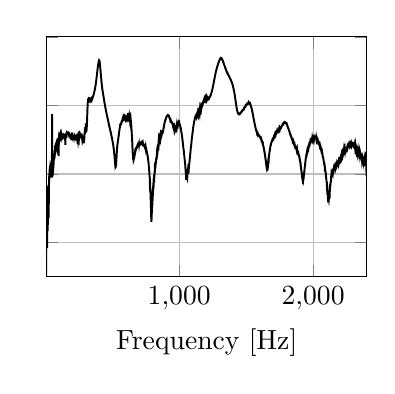
\begin{tikzpicture}

\begin{axis}[%
width=1.6in,
height=1.2in,
at={(1.011in,0.642in)},
scale only axis,
xmin=10,
xmax=2400,
xmajorgrids,
ymin=-30,
ymax=40,
ymajorgrids,
yticklabels={\empty},
xlabel={Frequency [Hz]},
axis background/.style={fill=white}
]
\addplot [color=black,solid,line width=0.7pt,forget plot]
  table[row sep=crcr]{%
0	-24.0538354294157\\
0.666675926054529	-24.7753265988161\\
1.33335185210906	-17.0382142167054\\
2.00002777816359	-18.7091958464009\\
2.66670370421811	-15.2032203403674\\
3.33337963027264	-8.53240216903954\\
4.00005555632717	-11.3881994991362\\
4.6667314823817	-7.34560264257265\\
5.33340740843623	-18.2635506378542\\
6.00008333449076	-30.0942089020284\\
6.66675926054529	-19.9100525240877\\
7.33343518659981	-21.3301429245582\\
8.00011111265434	-12.5504612701741\\
8.66678703870887	-15.3173206273707\\
9.3334629647634	-16.4624344447724\\
10.0001388908179	-21.0645945373479\\
10.6668148168725	-3.12818941832146\\
11.333490742927	-11.9814488880043\\
12.0001666689815	-16.3022691455521\\
12.666842595036	-16.83987041645\\
13.3335185210906	-21.5899394615097\\
14.0001944471451	-13.7669096045867\\
14.6668703731996	-10.7405701876275\\
15.3335462992542	-15.2513158642638\\
16.0002222253087	-12.4863764223308\\
16.6668981513632	-16.6735097060995\\
17.3335740774177	-11.1717261599997\\
18.0002500034723	-12.5642528883313\\
18.6669259295268	-14.7472480345922\\
19.3336018555813	-11.2309845901286\\
20.0002777816359	-12.3162845124428\\
20.6669537076904	-11.4989738149538\\
21.3336296337449	-11.4096075000397\\
22.0003055597994	-9.12000474667151\\
22.666981485854	-10.7058004870771\\
23.3336574119085	-10.8809274726073\\
24.000333337963	-12.8662435001899\\
24.6670092640176	-11.8084750036958\\
25.3336851900721	-9.39395341959846\\
26.0003611161266	-8.24921214045294\\
26.6670370421811	-5.13381010519183\\
27.3337129682357	-3.18474239145848\\
28.0003888942902	-1.96722097075604\\
28.6670648203447	-0.784435151267227\\
29.3337407463993	-0.564906469804107\\
30.0004166724538	-0.186628957762319\\
30.6670925985083	-0.223251397409185\\
31.3337685245628	-0.504288220825217\\
32.0004444506174	0.568981042424691\\
32.6671203766719	1.35135500831269\\
33.3337963027264	2.07752313968372\\
34.000472228781	2.13542686965292\\
34.6671481548355	1.87531635457994\\
35.33382408089	1.39408656672323\\
36.0005000069445	1.73767859557768\\
36.6671759329991	2.0365044287877\\
37.3338518590536	1.89103926658294\\
38.0005277851081	2.35267884483987\\
38.6672037111627	1.56785421692384\\
39.3338796372172	1.90575107773699\\
40.0005555632717	2.00696032260007\\
40.6672314893262	1.03747920044889\\
41.3339074153808	1.17819088709842\\
42.0005833414353	0.954423868100655\\
42.6672592674898	1.30215992319235\\
43.3339351935444	0.350798652357415\\
44.0006111195989	0.985446439692533\\
44.6672870456534	0.90853396189502\\
45.3339629717079	0.62363591607582\\
46.0006388977625	-0.106343649210524\\
46.667314823817	0.831296333741743\\
47.3339907498715	-0.154770617292899\\
48.0006666759261	-1.02488609973931\\
48.6673426019806	-0.349480793537451\\
49.3340185280351	1.40704941488586\\
50.0006944540896	17.4718617826514\\
50.6673703801442	-0.110905813330712\\
51.3340463061987	-0.969659382628823\\
52.0007222322532	-0.0156867446368573\\
52.6673981583078	-0.551828701230483\\
53.3340740843623	-0.335862030640212\\
54.0007500104168	-0.335709857720363\\
54.6674259364713	0.0689743844497208\\
55.3341018625259	0.149551305724914\\
56.0007777885804	0.650309261837628\\
56.6674537146349	0.13127845032964\\
57.3341296406895	0.572893104113807\\
58.000805566744	1.62672333434496\\
58.6674814927985	1.26340437511365\\
59.334157418853	1.80899399010958\\
60.0008333449076	2.12981393976939\\
60.6675092709621	2.11650037311116\\
61.3341851970166	2.70708359394901\\
62.0008611230712	3.0904031747816\\
62.6675370491257	3.73986090672288\\
63.3342129751802	4.11330532821165\\
64.0008889012347	4.28674048448287\\
64.6675648272893	4.49035790210038\\
65.3342407533438	4.62847704213878\\
66.0009166793983	4.90198327452499\\
66.6675926054529	5.40008752071958\\
67.3342685315074	5.71703775555609\\
68.0009444575619	5.85097210178158\\
68.6676203836164	6.35761681680145\\
69.334296309671	6.08420980880188\\
70.0009722357255	6.64342923814009\\
70.66764816178	7.14135937639171\\
71.3343240878346	6.95464466848458\\
72.0010000138891	7.3129468105897\\
72.6676759399436	7.26459405404091\\
73.3343518659981	7.48955717792348\\
74.0010277920527	7.65281470189807\\
74.6677037181072	7.55994571809288\\
75.3343796441617	7.89864326786307\\
76.0010555702163	7.63565632099739\\
76.6677314962708	7.89041771858883\\
77.3344074223253	7.83096423098779\\
78.0010833483798	7.95135021906428\\
78.6677592744344	8.15539545641694\\
79.3344352004889	8.08097874440249\\
80.0011111265434	8.18021272365017\\
80.667787052598	8.07561638981303\\
81.3344629786525	8.25782290136518\\
82.001138904707	8.02073159088786\\
82.6678148307615	8.42045087216576\\
83.3344907568161	8.1720438868478\\
84.0011666828706	8.11684485463587\\
84.6678426089251	8.2417824677993\\
85.3345185349797	8.26712476535566\\
86.0011944610342	8.08504729168952\\
86.6678703870887	8.39789867716215\\
87.3345463131432	8.45805928829301\\
88.0012222391978	8.62377756428815\\
88.6678981652523	8.52135557057066\\
89.3345740913068	8.67286525798598\\
90.0012500173614	8.85355762434988\\
90.6679259434159	9.00674645844902\\
91.3346018694704	9.00323229748388\\
92.0012777955249	9.23116144689982\\
92.6679537215795	9.19999321913624\\
93.334629647634	9.50702604628386\\
94.0013055736885	9.45354688509768\\
94.667981499743	9.60383675740148\\
95.3346574257976	9.70982758186113\\
96.0013333518521	9.81285612358788\\
96.6680092779066	9.87638222161103\\
97.3346852039612	9.98483507794277\\
98.0013611300157	10.2942179709114\\
98.6680370560702	10.0031320006568\\
99.3347129821248	10.234773264154\\
100.001388908179	5.20184010335849\\
100.668064834234	10.3673215378573\\
101.334740760288	10.6274246360448\\
102.001416686343	10.4963515327758\\
102.668092612397	10.6542180163706\\
103.334768538452	10.7270778119256\\
104.001444464506	10.7819900241968\\
104.668120390561	10.7476723911233\\
105.334796316616	10.8325568137231\\
106.00147224267	10.8565506329254\\
106.668148168725	10.7596885055515\\
107.334824094779	10.8153760411215\\
108.001500020834	10.9762515491244\\
108.668175946888	10.8813195235123\\
109.334851872943	10.9925472761605\\
110.001527798997	10.9839929711865\\
110.668203725052	10.8686273624886\\
111.334879651106	11.0336623311015\\
112.001555577161	10.8730227732298\\
112.668231503215	10.9764025968798\\
113.33490742927	10.9983924451575\\
114.001583355324	10.9932925852229\\
114.668259281379	10.8960860250767\\
115.334935207433	11.0971781560784\\
116.001611133488	10.9225306848365\\
116.668287059542	11.0012243151441\\
117.334962985597	10.9648906846422\\
118.001638911652	10.9810263450442\\
118.668314837706	10.9379766425556\\
119.334990763761	11.1180725359593\\
120.001666689815	10.8929973912361\\
120.66834261587	11.0346640034571\\
121.335018541924	11.0481488291843\\
122.001694467979	10.9418186978645\\
122.668370394033	10.9612899966686\\
123.335046320088	11.0949368089496\\
124.001722246142	11.0275110263947\\
124.668398172197	11.0715594833017\\
125.335074098251	11.0376539663672\\
126.001750024306	11.0892758690246\\
126.66842595036	10.9886866530624\\
127.335101876415	11.0544953488913\\
128.001777802469	11.086336614077\\
128.668453728524	11.0865827205247\\
129.335129654579	11.151384248337\\
130.001805580633	10.9699624040942\\
130.668481506688	11.0483383214513\\
131.335157432742	10.9434165920957\\
132.001833358797	10.9841995342106\\
132.668509284851	10.9498354463623\\
133.335185210906	11.0340101655261\\
134.00186113696	11.029981192541\\
134.668537063015	11.0002931400599\\
135.335212989069	11.0204717300212\\
136.001888915124	11.1082018634322\\
136.668564841178	11.1568604863805\\
137.335240767233	11.1212185688567\\
138.001916693287	11.1294445155704\\
138.668592619342	11.1038752994809\\
139.335268545396	10.9998777913079\\
140.001944471451	11.1203026571863\\
140.668620397506	11.0733110543624\\
141.33529632356	11.0783161713784\\
142.001972249615	11.2439397643653\\
142.668648175669	11.2245715123987\\
143.335324101724	11.2391735719326\\
144.002000027778	11.1714848438515\\
144.668675953833	11.2026579366728\\
145.335351879887	11.2800097757605\\
146.002027805942	11.2495634076332\\
146.668703731996	11.2875569503243\\
147.335379658051	11.2471604174122\\
148.002055584105	11.1433818238356\\
148.66873151016	11.1388023114834\\
149.335407436214	11.1083861020826\\
150.002083362269	8.49741873996997\\
150.668759288323	11.1444882241036\\
151.335435214378	11.0005689822991\\
152.002111140433	11.09039658558\\
152.668787066487	10.8554925363678\\
153.335462992542	10.8230173346571\\
154.002138918596	10.7685161320987\\
154.668814844651	10.8025435798439\\
155.335490770705	10.8135716851329\\
156.00216669676	10.8884190427297\\
156.668842622814	10.9438115197653\\
157.335518548869	11.108803501707\\
158.002194474923	11.3144993317585\\
158.668870400978	11.4290657039367\\
159.335546327032	11.5481305271641\\
160.002222253087	11.6743280140396\\
160.668898179141	11.5883742832391\\
161.335574105196	11.7607504814805\\
162.00225003125	11.7807862470171\\
162.668925957305	11.7467331034677\\
163.335601883359	11.7720285142441\\
164.002277809414	11.865060510984\\
164.668953735469	11.8803413440672\\
165.335629661523	11.8496811571761\\
166.002305587578	11.8324429598668\\
166.668981513632	11.8667775954332\\
167.335657439687	11.8685622372693\\
168.002333365741	11.9232402284661\\
168.669009291796	11.8631809517039\\
169.33568521785	11.8759285605512\\
170.002361143905	11.8500965787323\\
170.669037069959	11.8571411550248\\
171.335712996014	11.840672603201\\
172.002388922068	11.8726577669399\\
172.669064848123	11.8533596087701\\
173.335740774177	11.8970916548876\\
174.002416700232	11.8468821113692\\
174.669092626286	11.734120995521\\
175.335768552341	11.8545513954528\\
176.002444478396	11.8158272749587\\
176.66912040445	11.7581664010188\\
177.335796330505	11.6836690090809\\
178.002472256559	11.6134801753138\\
178.669148182614	11.545810162315\\
179.335824108668	11.580584591223\\
180.002500034723	11.4595817698421\\
180.669175960777	11.4109370365664\\
181.335851886832	11.4412280239627\\
182.002527812886	11.3337838862883\\
182.669203738941	11.2999958705124\\
183.335879664995	11.1766744105449\\
184.00255559105	11.2423046356787\\
184.669231517104	11.1506457429113\\
185.335907443159	11.049732946448\\
186.002583369213	11.0348385490678\\
186.669259295268	10.9294966777896\\
187.335935221323	10.9572626544397\\
188.002611147377	10.8441491005265\\
188.669287073432	10.7614007006402\\
189.335962999486	10.8383622788044\\
190.002638925541	10.8223907753729\\
190.669314851595	10.7318338151655\\
191.33599077765	10.7100341320297\\
192.002666703704	10.7954568913161\\
192.669342629759	10.7139401669828\\
193.336018555813	10.713553310691\\
194.002694481868	10.635326664087\\
194.669370407922	10.6914812192458\\
195.336046333977	10.6304543558945\\
196.002722260031	10.5135925535991\\
196.669398186086	10.4715652095356\\
197.33607411214	10.5958860446936\\
198.002750038195	10.5306409463711\\
198.66942596425	10.4646703088243\\
199.336101890304	10.6092591671541\\
200.002777816359	12.176381241264\\
200.669453742413	10.2229758071463\\
201.336129668468	10.4153000149645\\
202.002805594522	10.3409691366951\\
202.669481520577	10.3235299169775\\
203.336157446631	10.3908025729026\\
204.002833372686	10.4138955910993\\
204.66950929874	10.3096744183899\\
205.336185224795	10.3453530804593\\
206.002861150849	10.3411853460071\\
206.669537076904	10.4480086525697\\
207.336213002958	10.4821232768291\\
208.002888929013	10.4782237851814\\
208.669564855067	10.4857169071064\\
209.336240781122	10.5311820067122\\
210.002916707176	10.4065344665566\\
210.669592633231	10.3923410309562\\
211.336268559286	10.6125002075106\\
212.00294448534	10.6536877422631\\
212.669620411395	10.7075804710469\\
213.336296337449	10.5876450829407\\
214.002972263504	10.785798510488\\
214.669648189558	10.7575411253791\\
215.336324115613	10.8579433895683\\
216.003000041667	10.7564385534333\\
216.669675967722	10.8042910533961\\
217.336351893776	10.8590732035752\\
218.003027819831	10.9682998268144\\
218.669703745885	11.0298691531318\\
219.33637967194	10.9137424231625\\
220.003055597994	10.9268202865757\\
220.669731524049	11.1075459985888\\
221.336407450103	11.075272216335\\
222.003083376158	11.086723169469\\
222.669759302213	11.0306575287198\\
223.336435228267	11.0403269613152\\
224.003111154322	11.0461550610758\\
224.669787080376	10.8987251166676\\
225.336463006431	11.0093707380612\\
226.003138932485	11.0240270702722\\
226.66981485854	10.9899016358706\\
227.336490784594	10.8944098283972\\
228.003166710649	10.9776206027929\\
228.669842636703	10.9736768644323\\
229.336518562758	10.8881763913664\\
230.003194488812	10.8147798963354\\
230.669870414867	10.8177980422617\\
231.336546340921	10.8801157606152\\
232.003222266976	10.7283892320993\\
232.66989819303	10.6923124365478\\
233.336574119085	10.6786896011715\\
234.00325004514	10.4897476958619\\
234.669925971194	10.404416602913\\
235.336601897249	10.4085737009613\\
236.003277823303	10.3496630498464\\
236.669953749358	10.1939045392367\\
237.336629675412	10.3169473114109\\
238.003305601467	10.1109290157154\\
238.669981527521	10.0248242509185\\
239.336657453576	10.1248539008033\\
240.00333337963	9.86436784106379\\
240.670009305685	9.8461708563927\\
241.336685231739	9.80195907429479\\
242.003361157794	9.64681516121719\\
242.670037083848	9.65408983891004\\
243.336713009903	9.64755097355667\\
244.003388935957	9.47436381574311\\
244.670064862012	9.69859835886352\\
245.336740788066	9.54318354785978\\
246.003416714121	9.49157196217345\\
246.670092640176	9.61708331200281\\
247.33676856623	9.50254143555163\\
248.003444492285	9.58131774016605\\
248.670120418339	9.64528546865235\\
249.336796344394	9.58633365463329\\
250.003472270448	12.4050619191467\\
250.670148196503	10.1242217578109\\
251.336824122557	10.2671567123367\\
252.003500048612	10.562974536905\\
252.670175974666	10.6266234932955\\
253.336851900721	10.9711197026256\\
254.003527826775	10.9239309001141\\
254.67020375283	11.1999188615017\\
255.336879678884	11.1621178497936\\
256.003555604939	11.2330035027116\\
256.670231530993	11.3717480990161\\
257.336907457048	11.2397660539757\\
258.003583383103	11.3954434534165\\
258.670259309157	11.3330748055864\\
259.336935235212	11.4058114171549\\
260.003611161266	11.2727472424142\\
260.670287087321	11.3636069598555\\
261.336963013375	11.2803775781245\\
262.00363893943	11.3259731226633\\
262.670314865484	11.2831604198853\\
263.336990791539	11.2970077507477\\
264.003666717593	11.2537331196235\\
264.670342643648	11.2713568426248\\
265.337018569702	11.3038926896259\\
266.003694495757	11.1358976611144\\
266.670370421811	11.1288309856658\\
267.337046347866	11.0294360965846\\
268.00372227392	11.0311289283396\\
268.670398199975	11.0007018289668\\
269.33707412603	11.0526529539627\\
270.003750052084	10.9707716276467\\
270.670425978139	10.9747508530712\\
271.337101904193	10.6875614006601\\
272.003777830248	10.6611130565119\\
272.670453756302	10.5717850048715\\
273.337129682357	10.5648078472567\\
274.003805608411	10.499670336142\\
274.670481534466	10.3345037671487\\
275.33715746052	10.3743864040961\\
276.003833386575	10.0797133188244\\
276.670509312629	10.1874548657822\\
277.337185238684	9.99716266636554\\
278.003861164738	10.1329365143356\\
278.670537090793	9.9044650867058\\
279.337213016847	9.90190216469012\\
280.003888942902	9.79109249278751\\
280.670564868956	9.69492326926132\\
281.337240795011	9.69363522684118\\
282.003916721066	9.65539655977496\\
282.67059264712	9.61784377633952\\
283.337268573175	9.46150954678035\\
284.003944499229	9.4282426236971\\
284.670620425284	9.38794458809271\\
285.337296351338	9.3152770019253\\
286.003972277393	9.25769508223686\\
286.670648203447	9.19487404101757\\
287.337324129502	9.19501777667553\\
288.004000055556	9.35798780902652\\
288.670675981611	9.49456436606766\\
289.337351907665	9.7814876541983\\
290.00402783372	9.98147689201293\\
290.670703759774	10.2208175989873\\
291.337379685829	10.7311048602494\\
292.004055611883	11.0344757195201\\
292.670731537938	11.5192982400905\\
293.337407463993	11.8743752751125\\
294.004083390047	12.193556622589\\
294.670759316102	12.5652111611462\\
295.337435242156	12.9287677400434\\
296.004111168211	13.1378622004779\\
296.670787094265	13.2747682449318\\
297.33746302032	13.4282695085721\\
298.004138946374	13.5102474369325\\
298.670814872429	13.5312473320591\\
299.337490798483	13.3928499746803\\
300.004166724538	12.9948684163598\\
300.670842650592	13.3480927038971\\
301.337518576647	13.2475020503163\\
302.004194502701	13.0146629162693\\
302.670870428756	12.9962216245747\\
303.33754635481	12.8169344827781\\
304.004222280865	12.6361683472883\\
304.67089820692	12.5235804864241\\
305.337574132974	12.5701827364406\\
306.004250059029	12.4868789069686\\
306.670925985083	12.52032409134\\
307.337601911138	12.6466781948824\\
308.004277837192	12.9524182617077\\
308.670953763247	13.1715673652573\\
309.337629689301	13.5704043890882\\
310.004305615356	14.1606552716047\\
310.67098154141	14.7443826657853\\
311.337657467465	15.338294799873\\
312.004333393519	16.1663799368635\\
312.671009319574	16.9192556224687\\
313.337685245628	17.6011943590241\\
314.004361171683	18.3488092168469\\
314.671037097737	19.0888640542677\\
315.337713023792	19.6139738831932\\
316.004388949847	20.137762039088\\
316.671064875901	20.6552163789144\\
317.337740801956	20.9438530908394\\
318.00441672801	21.2412621975858\\
318.671092654065	21.4919486764409\\
319.337768580119	21.5977339205972\\
320.004444506174	21.7344452957731\\
320.671120432228	21.8822169758041\\
321.337796358283	21.9017537206537\\
322.004472284337	21.9473771938291\\
322.671148210392	22.0123528794745\\
323.337824136446	21.9793451486636\\
324.004500062501	22.0386109699524\\
324.671175988555	22.0408994279567\\
325.33785191461	21.9463862242842\\
326.004527840664	21.9753419819211\\
326.671203766719	21.933473132491\\
327.337879692774	21.875025790672\\
328.004555618828	21.8993855851231\\
328.671231544883	21.8122241818433\\
329.337907470937	21.7672598455656\\
330.004583396992	21.732754647684\\
330.671259323046	21.6567658373683\\
331.337935249101	21.6943787143949\\
332.004611175155	21.6311949762639\\
332.67128710121	21.5903275519017\\
333.337963027264	21.6334126166854\\
334.004638953319	21.4963114789822\\
334.671314879373	21.5484005574098\\
335.337990805428	21.5199247030615\\
336.004666731482	21.4870156650135\\
336.671342657537	21.544078906322\\
337.338018583591	21.4763389952504\\
338.004694509646	21.5451236206611\\
338.671370435701	21.5002992156288\\
339.338046361755	21.4914266245329\\
340.00472228781	21.5414916462764\\
340.671398213864	21.4969145634654\\
341.338074139919	21.5806730359757\\
342.004750065973	21.5164955323163\\
342.671425992028	21.631180114211\\
343.338101918082	21.6280672198441\\
344.004777844137	21.6524481284436\\
344.671453770191	21.6925161231834\\
345.338129696246	21.684657990614\\
346.0048056223	21.7959021361112\\
346.671481548355	21.7503780623695\\
347.338157474409	21.8858944759259\\
348.004833400464	21.8359367974069\\
348.671509326518	21.9503421196585\\
349.338185252573	21.9392384364729\\
350.004861178627	22.3870856318804\\
350.671537104682	22.0939943700624\\
351.338213030737	22.1333651372974\\
352.004888956791	22.1859159985505\\
352.671564882846	22.2314050905983\\
353.3382408089	22.3277504526568\\
354.004916734955	22.3332928147098\\
354.671592661009	22.456914580025\\
355.338268587064	22.5116795513418\\
356.004944513118	22.6268407556826\\
356.671620439173	22.6579767266709\\
357.338296365227	22.7830279539719\\
358.004972291282	22.7855363418947\\
358.671648217336	22.9282977061801\\
359.338324143391	22.9552004342005\\
360.005000069445	23.0967482034254\\
360.6716759955	23.1375534974305\\
361.338351921554	23.2671336898219\\
362.005027847609	23.3418111710958\\
362.671703773664	23.4712828577667\\
363.338379699718	23.553824857098\\
364.005055625773	23.6818063134887\\
364.671731551827	23.7736665359105\\
365.338407477882	23.8530357605844\\
366.005083403936	23.9997124292131\\
366.671759329991	24.0838168121703\\
367.338435256045	24.2347500113039\\
368.0051111821	24.3173935102669\\
368.671787108154	24.4909965246874\\
369.338463034209	24.558499138546\\
370.005138960263	24.7636680115791\\
370.671814886318	24.8500775519553\\
371.338490812372	25.0340991190821\\
372.005166738427	25.1554181253712\\
372.671842664481	25.31138732569\\
373.338518590536	25.503138701614\\
374.005194516591	25.5945440661062\\
374.671870442645	25.8258923739692\\
375.3385463687	25.8781832785756\\
376.005222294754	26.1212069673736\\
376.671898220809	26.2359863801086\\
377.338574146863	26.4563924416597\\
378.005250072918	26.6378861199214\\
378.671925998972	26.8034489554332\\
379.338601925027	27.0717627153897\\
380.005277851081	27.212045496638\\
380.671953777136	27.4561675539983\\
381.33862970319	27.6365587895402\\
382.005305629245	27.8153213652563\\
382.671981555299	28.0774413338392\\
383.338657481354	28.2342218562877\\
384.005333407408	28.5087659524338\\
384.672009333463	28.7540223326795\\
385.338685259517	28.9316679728972\\
386.005361185572	29.2350413994742\\
386.672037111627	29.3966621511991\\
387.338713037681	29.641209895069\\
388.005388963736	29.9193384375346\\
388.67206488979	30.0889819929086\\
389.338740815845	30.3889089301848\\
390.005416741899	30.5834284748198\\
390.672092667954	30.7520419489202\\
391.338768594008	31.0253306189734\\
392.005444520063	31.1691438622083\\
392.672120446117	31.3805029492705\\
393.338796372172	31.6109791175107\\
394.005472298226	31.7088394068235\\
394.672148224281	31.8977166816165\\
395.338824150335	32.118590197554\\
396.00550007639	32.2250301442221\\
396.672176002444	32.4383969709178\\
397.338851928499	32.584372014053\\
398.005527854554	32.652834316717\\
398.672203780608	32.8554270618435\\
399.338879706663	32.9949422192336\\
400.005555632717	33.0478065427637\\
400.672231558772	33.1054097052581\\
401.338907484826	33.2000438623887\\
402.005583410881	33.1679382029102\\
402.672259336935	33.1553109660612\\
403.33893526299	33.148151872368\\
404.005611189044	33.0332835311622\\
404.672287115099	32.9205788736783\\
405.338963041153	32.810301879351\\
406.005638967208	32.5985487610059\\
406.672314893262	32.3851116469242\\
407.338990819317	32.2026022497992\\
408.005666745371	31.9559744308648\\
408.672342671426	31.6418704159758\\
409.339018597481	31.3864409761776\\
410.005694523535	31.1469497092695\\
410.67237044959	30.7977082329506\\
411.339046375644	30.4783875394015\\
412.005722301699	30.2433520025839\\
412.672398227753	29.9082916554792\\
413.339074153808	29.5561508893066\\
414.005750079862	29.2914123673672\\
414.672426005917	29.0006488166639\\
415.339101931971	28.6876653242218\\
416.005777858026	28.3640825702083\\
416.67245378408	28.0606596600821\\
417.339129710135	27.8503313282515\\
418.005805636189	27.5189732830465\\
418.672481562244	27.1808685798042\\
419.339157488298	26.9525030135891\\
420.005833414353	26.7409332472361\\
420.672509340407	26.4505140133333\\
421.339185266462	26.1373778956874\\
422.005861192517	25.9445242047876\\
422.672537118571	25.7238560344385\\
423.339213044626	25.5265166116736\\
424.00588897068	25.2491125724447\\
424.672564896735	25.0250081623613\\
425.339240822789	24.8974975226114\\
426.005916748844	24.7224643389561\\
426.672592674898	24.5006868441122\\
427.339268600953	24.3066994958521\\
428.005944527007	24.1462413550494\\
428.672620453062	24.0507375112873\\
429.339296379116	23.8892840468726\\
430.005972305171	23.6776851026303\\
430.672648231225	23.5099653059884\\
431.33932415728	23.3478236259535\\
432.006000083334	23.2364127595894\\
432.672676009389	23.1207612587907\\
433.339351935444	22.8959361913742\\
434.006027861498	22.7471931522182\\
434.672703787553	22.5433582405117\\
435.339379713607	22.4547303842041\\
436.006055639662	22.2914653457661\\
436.672731565716	22.1519722574286\\
437.339407491771	21.9399191349777\\
438.006083417825	21.7290116106934\\
438.67275934388	21.5988691511031\\
439.339435269934	21.4594341238752\\
440.006111195989	21.3562168861861\\
440.672787122043	21.144900900334\\
441.339463048098	20.9739586695309\\
442.006138974152	20.7736080862848\\
442.672814900207	20.6201277638556\\
443.339490826261	20.5023998974435\\
444.006166752316	20.389707420288\\
444.672842678371	20.2221190500421\\
445.339518604425	20.1150004192628\\
446.00619453048	19.8958868027358\\
446.672870456534	19.7185496925901\\
447.339546382589	19.5946554813454\\
448.006222308643	19.4447782425543\\
448.672898234698	19.3248187746355\\
449.339574160752	19.2415878026817\\
450.006250086807	19.1969702927045\\
450.672926012861	18.9235712221156\\
451.339601938916	18.786476495092\\
452.00627786497	18.6138438464368\\
452.672953791025	18.458029742538\\
453.339629717079	18.3735391635682\\
454.006305643134	18.2274483277047\\
454.672981569188	18.1198667818157\\
455.339657495243	17.9970599081178\\
456.006333421298	17.9104914480584\\
456.673009347352	17.7908964404868\\
457.339685273407	17.6300876671202\\
458.006361199461	17.5205393224243\\
458.673037125516	17.3789005038587\\
459.33971305157	17.219497155265\\
460.006388977625	17.0916857427261\\
460.673064903679	16.967776133388\\
461.339740829734	16.8481704528801\\
462.006416755788	16.7606037216756\\
462.673092681843	16.6287300042932\\
463.339768607897	16.5150807513815\\
464.006444533952	16.4335668264479\\
464.673120460006	16.3541986927064\\
465.339796386061	16.2444898512573\\
466.006472312115	16.1022276577805\\
466.67314823817	16.0099998689133\\
467.339824164225	15.8321201445416\\
468.006500090279	15.731463989389\\
468.673176016334	15.598667407565\\
469.339851942388	15.4434925118285\\
470.006527868443	15.3418255048297\\
470.673203794497	15.260400829156\\
471.339879720552	15.1028294124931\\
472.006555646606	14.9703269586253\\
472.673231572661	14.8720922816024\\
473.339907498715	14.7048017505083\\
474.00658342477	14.6348712133549\\
474.673259350824	14.5046704313732\\
475.339935276879	14.3409902316396\\
476.006611202933	14.2909428993713\\
476.673287128988	14.1090275349316\\
477.339963055042	13.9893366679867\\
478.006638981097	13.9396784257778\\
478.673314907152	13.8030625702837\\
479.339990833206	13.6464528292807\\
480.006666759261	13.6262442302645\\
480.673342685315	13.4337902085009\\
481.34001861137	13.2908180780304\\
482.006694537424	13.2238446919687\\
482.673370463479	13.1087385153536\\
483.340046389533	12.9774902252141\\
484.006722315588	12.9235558923937\\
484.673398241642	12.7797322506448\\
485.340074167697	12.6652555108802\\
486.006750093751	12.5296361654673\\
486.673426019806	12.4705219488855\\
487.34010194586	12.3409420524972\\
488.006777871915	12.1918314613151\\
488.673453797969	12.1237800371845\\
489.340129724024	12.1137693010676\\
490.006805650078	11.9399408447004\\
490.673481576133	11.7769438523611\\
491.340157502188	11.6521991299404\\
492.006833428242	11.5335559889926\\
492.673509354297	11.3711021779641\\
493.340185280351	11.2797519092352\\
494.006861206406	11.1450543787188\\
494.67353713246	11.0490224157538\\
495.340213058515	10.8802703470087\\
496.006888984569	10.6657933239491\\
496.673564910624	10.639583194267\\
497.340240836678	10.5331311702954\\
498.006916762733	10.4376658346226\\
498.673592688787	10.226261189877\\
499.340268614842	10.173280789518\\
500.006944540896	9.97658207157796\\
500.673620466951	9.93104255542565\\
501.340296393005	9.70299151470093\\
502.00697231906	9.56427842467682\\
502.673648245115	9.40966460679045\\
503.340324171169	9.23208529134278\\
504.007000097224	9.16591247293168\\
504.673676023278	9.02470332922051\\
505.340351949333	8.85799847535677\\
506.007027875387	8.68232112750533\\
506.673703801442	8.49015542367151\\
507.340379727496	8.35612313467402\\
508.007055653551	8.09827396310981\\
508.673731579605	7.95619332879397\\
509.34040750566	7.71668486249847\\
510.007083431714	7.54408425757578\\
510.673759357769	7.3866368832407\\
511.340435283823	7.20454326168255\\
512.007111209878	6.96606098465922\\
512.673787135932	6.72619901342163\\
513.340463061987	6.33214482749454\\
514.007138988041	6.09664452506388\\
514.673814914096	6.00821140207314\\
515.340490840151	5.68996033058963\\
516.007166766205	5.41891292066807\\
516.67384269226	5.19913029101021\\
517.340518618314	4.74641232196898\\
518.007194544369	4.44353283286356\\
518.673870470423	4.18881886188834\\
519.340546396478	3.84761742946598\\
520.007222322532	3.53418988119992\\
520.673898248587	3.14939886494411\\
521.340574174641	2.838292842742\\
522.007250100696	2.57379153395263\\
522.67392602675	2.68621460723454\\
523.340601952805	2.54268561550195\\
524.007277878859	2.44119387057222\\
524.673953804914	2.34546990210759\\
525.340629730968	2.12788718992\\
526.007305657023	2.17247785298671\\
526.673981583078	2.17437754975731\\
527.340657509132	2.30955463293454\\
528.007333435187	2.32552210191851\\
528.674009361241	2.56150916661386\\
529.340685287296	3.1056710717391\\
530.00736121335	3.77675628169621\\
530.674037139405	4.23542156703512\\
531.340713065459	4.5715970853357\\
532.007388991514	4.98174110027376\\
532.674064917568	5.72223246797755\\
533.340740843623	6.01634248893307\\
534.007416769677	6.40373719646523\\
534.674092695732	6.81682238561117\\
535.340768621786	7.17875928125927\\
536.007444547841	7.47873462105253\\
536.674120473896	7.80929354526687\\
537.34079639995	8.05245706986005\\
538.007472326005	8.36022547474432\\
538.674148252059	8.58557421707928\\
539.340824178114	8.81462764879022\\
540.007500104168	8.93724767281927\\
540.674176030223	9.30767053508195\\
541.340851956277	9.41314167146452\\
542.007527882332	9.55514198421905\\
542.674203808386	9.80504696603795\\
543.340879734441	10.0715779624224\\
544.007555660495	10.1903989708205\\
544.67423158655	10.3261730853789\\
545.340907512604	10.5231373859331\\
546.007583438659	10.7373606145697\\
546.674259364713	10.8528441788335\\
547.340935290768	11.0243072468929\\
548.007611216823	11.3312786158819\\
548.674287142877	11.3774764740178\\
549.340963068932	11.6524856563262\\
550.007638994986	11.8209336106523\\
550.674314921041	12.0719428085404\\
551.340990847095	12.174427441001\\
552.00766677315	12.4054022511678\\
552.674342699204	12.675640934017\\
553.341018625259	12.8103604363372\\
554.007694551313	12.9886014144124\\
554.674370477368	13.1767125315813\\
555.341046403422	13.3030478639295\\
556.007722329477	13.4715164884348\\
556.674398255531	13.7083858707781\\
557.341074181586	13.7995387628935\\
558.00775010764	13.9282687496593\\
558.674426033695	14.2224926371625\\
559.341101959749	14.2258110595647\\
560.007777885804	14.3252407459023\\
560.674453811858	14.5106403874977\\
561.341129737913	14.5096064949592\\
562.007805663968	14.5862548783372\\
562.674481590022	14.6686389667934\\
563.341157516077	14.668275787313\\
564.007833442131	14.7581885840426\\
564.674509368186	14.7889406640586\\
565.34118529424	14.7330637771831\\
566.007861220295	14.7761720485605\\
566.674537146349	14.7950379349273\\
567.341213072404	14.8136528998632\\
568.007888998458	14.9307479037634\\
568.674564924513	14.8869093992123\\
569.341240850567	15.0020057804691\\
570.007916776622	15.0448899036403\\
570.674592702676	15.0733428753757\\
571.341268628731	15.2653123767828\\
572.007944554785	15.2859544262324\\
572.67462048084	15.3244107965716\\
573.341296406895	15.5056585597125\\
574.007972332949	15.5463222031134\\
574.674648259004	15.7091986008417\\
575.341324185058	15.7857704631097\\
576.008000111113	15.8942386542656\\
576.674676037167	16.0257081173392\\
577.341351963222	16.0149498355079\\
578.008027889276	16.1879588740618\\
578.674703815331	16.1729269420844\\
579.341379741385	16.3083726802466\\
580.00805566744	16.3575588369278\\
580.674731593494	16.365937703832\\
581.341407519549	16.4928648069782\\
582.008083445603	16.4135098039103\\
582.674759371658	16.5606232989547\\
583.341435297712	16.4949869606825\\
584.008111223767	16.5875942777116\\
584.674787149822	16.5514655794609\\
585.341463075876	16.5654555789107\\
586.008139001931	16.6053193123706\\
586.674814927985	16.5052009636011\\
587.34149085404	16.6072309414191\\
588.008166780094	16.4786187578352\\
588.674842706149	16.5574939792168\\
589.341518632203	16.4367798218283\\
590.008194558258	16.4995798511669\\
590.674870484312	16.3865012367849\\
591.341546410367	16.4592085148972\\
592.008222336421	16.340487948373\\
592.674898262476	16.3670572759151\\
593.34157418853	16.3063615038774\\
594.008250114585	16.3455728584197\\
594.674926040639	16.2608916229011\\
595.341601966694	16.297350941732\\
596.008277892749	16.2025084546167\\
596.674953818803	16.2378002755367\\
597.341629744858	16.1963992046452\\
598.008305670912	16.1688825705917\\
598.674981596967	16.1131426357601\\
599.341657523021	16.2063396706033\\
600.008333449076	16.082470288651\\
600.67500937513	16.1749020334652\\
601.341685301185	16.1246008212953\\
602.008361227239	16.1984115744638\\
602.675037153294	16.0948019285334\\
603.341713079348	16.2170131537778\\
604.008389005403	16.1304315172695\\
604.675064931457	16.2492579274956\\
605.341740857512	16.1712036728509\\
606.008416783566	16.2362173440111\\
606.675092709621	16.2120105909438\\
607.341768635676	16.3022758438576\\
608.00844456173	16.2397755587875\\
608.675120487785	16.3371921941228\\
609.341796413839	16.3336724777239\\
610.008472339894	16.3313353363035\\
610.675148265948	16.3979196428623\\
611.341824192003	16.3129768461316\\
612.008500118057	16.4385269611059\\
612.675176044112	16.3194257948107\\
613.341851970166	16.4457013711349\\
614.008527896221	16.4065585931307\\
614.675203822275	16.4363597931761\\
615.34187974833	16.507449764277\\
616.008555674384	16.4506796275132\\
616.675231600439	16.5520510315926\\
617.341907526493	16.4627257345375\\
618.008583452548	16.624553047341\\
618.675259378603	16.5335960648416\\
619.341935304657	16.5616368108617\\
620.008611230711	16.636736390542\\
620.675287156766	16.5478634227533\\
621.341963082821	16.6756072286469\\
622.008639008875	16.5836004908967\\
622.67531493493	16.6108910965367\\
623.341990860984	16.6894703602389\\
624.008666787039	16.5677177530767\\
624.675342713093	16.6913117157591\\
625.342018639148	16.6488815610008\\
626.008694565202	16.5487677436973\\
626.675370491257	16.7555897507216\\
627.342046417311	16.55274074888\\
628.008722343366	16.5611432576366\\
628.67539826942	16.6416552804713\\
629.342074195475	16.4320030957751\\
630.008750121529	16.5406189712251\\
630.675426047584	16.580535623175\\
631.342101973638	16.267797586175\\
632.008777899693	16.4726226747189\\
632.675453825748	16.4025795355512\\
633.342129751802	16.1751980714638\\
634.008805677857	16.2920847485297\\
634.675481603911	16.0718224148971\\
635.342157529966	15.9247024759311\\
636.00883345602	16.0239536112237\\
636.675509382075	15.799687708656\\
637.342185308129	15.4575806981259\\
638.008861234184	15.6327066208098\\
638.675537160238	15.3118732652641\\
639.342213086293	14.8517393760472\\
640.008889012347	14.9662407330703\\
640.675564938402	14.7259462068026\\
641.342240864456	14.1296834286275\\
642.008916790511	13.9712980107766\\
642.675592716565	13.9101024775435\\
643.34226864262	13.1266704172734\\
644.008944568675	12.8538851703094\\
644.675620494729	12.7481594386484\\
645.342296420784	11.9965695483298\\
646.008972346838	11.4499069847361\\
646.675648272893	11.2990796911129\\
647.342324198947	10.7009231507117\\
648.009000125002	9.88953406030728\\
648.675676051056	9.50168700273076\\
649.342351977111	9.10954130375459\\
650.009027903165	8.64820776820932\\
650.67570382922	7.61756872242853\\
651.342379755274	7.40586741417076\\
652.009055681329	7.08942540282487\\
652.675731607383	6.08200626385361\\
653.342407533438	5.72419650143808\\
654.009083459492	5.49759242816381\\
654.675759385547	5.29169501571504\\
655.342435311602	4.71109730366877\\
656.009111237656	4.29505478873706\\
656.675787163711	4.61234146286363\\
657.342463089765	4.51977411033579\\
658.00913901582	4.24545086492994\\
658.675814941874	3.99616888525082\\
659.342490867929	4.07913016147592\\
660.009166793983	4.43900944385735\\
660.675842720038	4.38012170617682\\
661.342518646092	4.4514484809695\\
662.009194572147	4.55053847636848\\
662.675870498201	4.68581788631672\\
663.342546424256	5.06836396711243\\
664.00922235031	5.03834687003778\\
664.675898276365	5.01798182971722\\
665.342574202419	5.29255886284392\\
666.009250128474	5.57963088869587\\
666.675926054529	5.70082816841368\\
667.342601980583	5.66047564216475\\
668.009277906638	5.65110414379459\\
668.675953832692	6.05820324551451\\
669.342629758747	6.26256346656145\\
670.009305684801	6.18875699485358\\
670.675981610856	6.26566083216555\\
671.34265753691	6.37375958455085\\
672.009333462965	6.46899287385204\\
672.676009389019	6.7023481501977\\
673.342685315074	6.92994514722064\\
674.009361241128	6.9142441838001\\
674.676037167183	6.84390413844429\\
675.342713093237	6.93362228437308\\
676.009389019292	7.16013982468008\\
676.676064945346	7.29782724821155\\
677.342740871401	7.28099887468422\\
678.009416797456	7.28553560396656\\
678.67609272351	7.3438589447758\\
679.342768649565	7.35268456383873\\
680.009444575619	7.46013201228345\\
680.676120501674	7.58787823875755\\
681.342796427728	7.70987056832242\\
682.009472353783	7.7047698036689\\
682.676148279837	7.71836181754712\\
683.342824205892	7.71287810866602\\
684.009500131946	7.88491955520567\\
684.676176058001	7.88200458566801\\
685.342851984055	7.97871547719071\\
686.00952791011	8.06262035838028\\
686.676203836164	8.19454833038218\\
687.342879762219	8.16680871449154\\
688.009555688273	8.14986629672043\\
688.676231614328	8.11098997869995\\
689.342907540382	8.15600053376475\\
690.009583466437	8.2431174413041\\
690.676259392492	8.35857584547801\\
691.342935318546	8.47980551964391\\
692.009611244601	8.43020986419829\\
692.676287170655	8.48780149220811\\
693.34296309671	8.49475492350756\\
694.009639022764	8.48315887279011\\
694.676314948819	8.50345618383611\\
695.342990874873	8.48156685248925\\
696.009666800928	8.6273150299049\\
696.676342726982	8.65591179059107\\
697.343018653037	8.66517613107\\
698.009694579091	8.77821021920323\\
698.676370505146	8.75333557717898\\
699.3430464312	8.8738621831423\\
700.009722357255	8.65908011082201\\
700.676398283309	8.86688296460674\\
701.343074209364	8.99292078768806\\
702.009750135419	8.92702794124702\\
702.676426061473	8.94314707926746\\
703.343101987528	9.00448341199101\\
704.009777913582	8.99974507269237\\
704.676453839637	8.94855984341114\\
705.343129765691	8.91491375340969\\
706.009805691746	9.04507061596649\\
706.6764816178	9.03253887450496\\
707.343157543855	9.0075023601351\\
708.009833469909	8.99718959363287\\
708.676509395964	9.10477017565572\\
709.343185322018	9.17907052885568\\
710.009861248073	9.18639911781509\\
710.676537174127	9.08239240901507\\
711.343213100182	9.16189627843021\\
712.009889026236	9.19475262476087\\
712.676564952291	9.2117120724423\\
713.343240878346	9.24617414557119\\
714.0099168044	9.28100228694381\\
714.676592730455	9.3022214295608\\
715.343268656509	9.21367630460709\\
716.009944582564	9.22161749744294\\
716.676620508618	9.20051200364815\\
717.343296434673	9.19917213365312\\
718.009972360727	9.20628728333848\\
718.676648286782	9.15288523255609\\
719.343324212836	9.18144019305628\\
720.010000138891	9.0888488044096\\
720.676676064945	9.13366907544728\\
721.343351991	9.09691399403723\\
722.010027917054	9.07780768358352\\
722.676703843109	8.99477464928745\\
723.343379769163	9.06415786331838\\
724.010055695218	8.9396147449063\\
724.676731621273	8.91679571829932\\
725.343407547327	8.89078643803618\\
726.010083473382	8.89081486731126\\
726.676759399436	8.86587058208948\\
727.343435325491	8.82387149713632\\
728.010111251545	8.84742213310955\\
728.6767871776	8.80797109096137\\
729.343463103654	8.77921127750227\\
730.010139029709	8.88600239733476\\
730.676814955763	8.76052369591128\\
731.343490881818	8.84503878959984\\
732.010166807872	8.78348576588829\\
732.676842733927	8.74729278566041\\
733.343518659981	8.69718510731511\\
734.010194586036	8.58765820005153\\
734.67687051209	8.55866789218656\\
735.343546438145	8.57966892515378\\
736.0102223642	8.51429485733572\\
736.676898290254	8.47576228049317\\
737.343574216309	8.47350178943034\\
738.010250142363	8.36534874926045\\
738.676926068418	8.3134314464271\\
739.343601994472	8.30784562333557\\
740.010277920527	8.30356706532026\\
740.676953846581	8.29810828413785\\
741.343629772636	8.28230145879134\\
742.01030569869	8.19757323542451\\
742.676981624745	8.16306820019938\\
743.343657550799	8.10197498872195\\
744.010333476854	7.91140718178206\\
744.677009402908	7.95146581159202\\
745.343685328963	7.89349505820059\\
746.010361255017	7.81561049766296\\
746.677037181072	7.91101046118437\\
747.343713107127	7.81549474148716\\
748.010389033181	7.79004878356179\\
748.677064959236	7.66829467356041\\
749.34374088529	7.49522738347616\\
750.010416811345	7.68306725636067\\
750.677092737399	7.47542347743726\\
751.343768663454	7.30539756747948\\
752.010444589508	7.32444285285847\\
752.677120515563	7.19256018569224\\
753.343796441617	7.22101513454485\\
754.010472367672	6.98367788213361\\
754.677148293726	6.94151082884162\\
755.343824219781	6.81920124364684\\
756.010500145835	6.85561208875995\\
756.67717607189	6.73901309068327\\
757.343851997944	6.65447059917736\\
758.010527923999	6.39940819849267\\
758.677203850054	6.31537062804607\\
759.343879776108	6.2304774693665\\
760.010555702162	6.15132302820454\\
760.677231628217	6.03645142947089\\
761.343907554272	5.82856391160883\\
762.010583480326	5.62639500122763\\
762.677259406381	5.49140195078828\\
763.343935332435	5.29501650067733\\
764.01061125849	5.28840291402563\\
764.677287184544	5.13659478264419\\
765.343963110599	4.92696956390757\\
766.010639036653	4.65854266888813\\
766.677314962708	4.49329801241826\\
767.343990888762	4.39946911523809\\
768.010666814817	4.1882380007889\\
768.677342740871	3.83121132007652\\
769.344018666926	3.6747490934063\\
770.01069459298	3.51415478445073\\
770.677370519035	3.36285311572927\\
771.344046445089	2.99118916014252\\
772.010722371144	2.83533387759084\\
772.677398297199	2.31556653261333\\
773.344074223253	2.18825393175463\\
774.010750149308	1.94755390900186\\
774.677426075362	1.30582271184568\\
775.344102001417	1.12798424630628\\
776.010777927471	1.11609012507506\\
776.677453853526	0.541390822703892\\
777.34412977958	0.158386409686359\\
778.010805705635	-0.468980051040267\\
778.677481631689	-0.714193168197218\\
779.344157557744	-0.899055137537588\\
780.010833483798	-1.07703919157975\\
780.677509409853	-2.49646867206346\\
781.344185335907	-2.37501600216951\\
782.010861261962	-2.17316165963422\\
782.677537188016	-4.0581005908558\\
783.344213114071	-4.58062890864723\\
784.010889040126	-4.58269787118991\\
784.67756496618	-4.7208140869024\\
785.344240892235	-5.73279953533563\\
786.010916818289	-6.89575411330063\\
786.677592744344	-6.68381994855648\\
787.344268670398	-8.18517020034133\\
788.010944596453	-9.90652762988221\\
788.677620522507	-8.18289582525946\\
789.344296448562	-10.1846467980253\\
790.010972374616	-12.5734242530755\\
790.677648300671	-11.2925063282194\\
791.344324226725	-11.0326681826804\\
792.01100015278	-13.9522799585502\\
792.677676078834	-10.6894138613858\\
793.344352004889	-11.2152910111612\\
794.011027930943	-13.2516412128331\\
794.677703856998	-9.79569996931918\\
795.344379783053	-11.3022395543273\\
796.011055709107	-11.4952272503209\\
796.677731635162	-8.41722339018986\\
797.344407561216	-9.72627220711398\\
798.011083487271	-9.94979243639554\\
798.677759413325	-6.87502790192122\\
799.34443533938	-9.12375254882056\\
800.011111265434	-7.32160601680179\\
800.677787191489	-5.43797021337587\\
801.344463117543	-7.80256595429727\\
802.011139043598	-5.13409187346906\\
802.677814969652	-4.94108863994887\\
803.344490895707	-6.37745787416539\\
804.011166821761	-3.55950243852837\\
804.677842747816	-4.30586109253226\\
805.34451867387	-4.59397551263602\\
806.011194599925	-2.73093805028424\\
806.67787052598	-4.50721520541811\\
807.344546452034	-2.71904955651304\\
808.011222378089	-2.56406630580553\\
808.677898304143	-3.79276753181882\\
809.344574230198	-1.43233406110157\\
810.011250156252	-2.40888422001714\\
810.677926082307	-2.26245578595983\\
811.344602008361	-1.04421395839191\\
812.011277934416	-2.49516241499997\\
812.67795386047	-0.268917971359419\\
813.344629786525	-1.44027205880575\\
814.011305712579	-0.58017509754626\\
814.677981638634	-0.106411658385477\\
815.344657564688	-0.604591426118682\\
816.011333490743	0.94649791000057\\
816.678009416797	-0.0135856302018601\\
817.344685342852	1.01227256578035\\
818.011361268907	0.874174188656179\\
818.678037194961	1.14296528929029\\
819.344713121016	1.83339816048708\\
820.01138904707	1.37241871192462\\
820.678064973125	2.35754556263054\\
821.344740899179	1.695533751534\\
822.011416825234	2.65437077751505\\
822.678092751288	2.33195299209198\\
823.344768677343	2.6712027563085\\
824.011444603397	3.12226968652874\\
824.678120529452	2.85017726099925\\
825.344796455506	3.68194181903176\\
826.011472381561	3.10750420962551\\
826.678148307615	4.10803459146397\\
827.34482423367	3.63804406996872\\
828.011500159724	4.50743894422469\\
828.678176085779	4.26625290414105\\
829.344852011833	4.5765990683043\\
830.011527937888	4.72375359303579\\
830.678203863943	4.97318854745414\\
831.344879789997	5.04487623377831\\
832.011555716052	5.21440337067422\\
832.678231642106	5.4887612967534\\
833.344907568161	5.62068819776284\\
834.011583494215	6.0910417712059\\
834.67825942027	5.98735626527823\\
835.344935346324	6.328626218188\\
836.011611272379	6.43646375962649\\
836.678287198433	6.7736958348463\\
837.344963124488	6.82165695424229\\
838.011639050542	7.19372361307892\\
838.678314976597	7.11523922481778\\
839.344990902651	7.57138139653562\\
840.011666828706	7.557247900819\\
840.67834275476	7.90611873433456\\
841.345018680815	7.91608176675178\\
842.01169460687	8.09851421262908\\
842.678370532924	8.3536357220389\\
843.345046458979	8.40510316993884\\
844.011722385033	8.67827879791309\\
844.678398311088	8.72842127719789\\
845.345074237142	9.06145967026124\\
846.011750163197	8.85824675407166\\
846.678426089251	9.33381122591847\\
847.345102015306	9.16247240374297\\
848.01177794136	9.53714993615979\\
848.678453867415	9.45222110064775\\
849.345129793469	9.75549204802832\\
850.011805719524	9.72011555940689\\
850.678481645578	9.80556141254699\\
851.345157571633	10.0157705307232\\
852.011833497687	9.98782400806894\\
852.678509423742	10.3263323152393\\
853.345185349797	10.2263075124648\\
854.011861275851	10.4673662333594\\
854.678537201906	10.4750122257284\\
855.34521312796	10.5812683543939\\
856.011889054015	10.7432021798873\\
856.678564980069	10.6224034655495\\
857.345240906124	10.8200206780487\\
858.011916832178	10.7909061950638\\
858.678592758233	10.9237707622318\\
859.345268684287	11.0856784961665\\
860.011944610342	10.8644352842758\\
860.678620536396	11.1261066554508\\
861.345296462451	11.0244524327826\\
862.011972388505	11.1470113009769\\
862.67864831456	11.2547196785471\\
863.345324240614	11.0448320287065\\
864.012000166669	11.2151192729638\\
864.678676092724	11.2531785369515\\
865.345352018778	11.2555770207634\\
866.012027944833	11.4987110031993\\
866.678703870887	11.4224990994646\\
867.345379796942	11.5779639905364\\
868.012055722996	11.640257357955\\
868.678731649051	11.6007867483666\\
869.345407575105	11.781237805192\\
870.01208350116	11.877495251888\\
870.678759427214	11.8489151436538\\
871.345435353269	12.0846483711101\\
872.012111279323	12.0525281222913\\
872.678787205378	12.0139984235166\\
873.345463131432	12.0826812209638\\
874.012139057487	12.061523307729\\
874.678814983541	12.1489753287143\\
875.345490909596	12.3037009790466\\
876.012166835651	12.3632402363005\\
876.678842761705	12.3976444803187\\
877.34551868776	12.5413102336594\\
878.012194613814	12.5428786333715\\
878.678870539869	12.5052739178201\\
879.345546465923	12.6803526763113\\
880.012222391978	12.7657815401847\\
880.678898318032	12.7619737549631\\
881.345574244087	12.9302223410476\\
882.012250170141	13.1298104776297\\
882.678926096196	13.1343444772437\\
883.34560202225	13.3622493754369\\
884.012277948305	13.516955430761\\
884.678953874359	13.628462736946\\
885.345629800414	13.7511746464535\\
886.012305726468	13.9753184008757\\
886.678981652523	14.1028982643568\\
887.345657578578	14.1752525376684\\
888.012333504632	14.4232471395254\\
888.679009430687	14.6262802091452\\
889.345685356741	14.6695853406587\\
890.012361282796	14.8377869147203\\
890.67903720885	14.9993208078014\\
891.345713134905	15.0808226015919\\
892.012389060959	15.1835072151555\\
892.679064987014	15.2992595795399\\
893.345740913068	15.4770778589417\\
894.012416839123	15.5313052994013\\
894.679092765177	15.5677504345894\\
895.345768691232	15.6845822811017\\
896.012444617286	15.7420524263474\\
896.679120543341	15.7676966606647\\
897.345796469395	15.7644520748567\\
898.01247239545	15.8820572624777\\
898.679148321504	15.9725363968445\\
899.345824247559	16.0137849317211\\
900.012500173613	16.085611690765\\
900.679176099668	16.1409539861349\\
901.345852025723	16.2961684756008\\
902.012527951777	16.3377643610367\\
902.679203877832	16.4297773781262\\
903.345879803886	16.4858328512957\\
904.012555729941	16.564890281754\\
904.679231655995	16.6877664339662\\
905.34590758205	16.7312284524711\\
906.012583508104	16.7491872727016\\
906.679259434159	16.8286310282731\\
907.345935360213	16.8741824254074\\
908.012611286268	16.9141639567492\\
908.679287212322	16.9528059124308\\
909.345963138377	17.0085270302337\\
910.012639064431	17.0507269149622\\
910.679314990486	17.0919263331357\\
911.34599091654	17.1157916064077\\
912.012666842595	17.1178820583425\\
912.67934276865	17.0880992386827\\
913.346018694704	17.1412446050638\\
914.012694620759	17.1206095613056\\
914.679370546813	17.157389034818\\
915.346046472868	17.1386740071617\\
916.012722398922	17.1253703278769\\
916.679398324977	17.1517005258387\\
917.346074251031	17.1273425555082\\
918.012750177086	17.1681988564691\\
918.67942610314	17.1485984223438\\
919.346102029195	17.1222604286733\\
920.012777955249	17.0702448417329\\
920.679453881304	17.0327124157506\\
921.346129807358	17.0239384095614\\
922.012805733413	16.9688121297861\\
922.679481659467	16.9417438457129\\
923.346157585522	16.9388097335481\\
924.012833511577	16.8382022700095\\
924.679509437631	16.7353323309267\\
925.346185363686	16.6337259820966\\
926.01286128974	16.5335111732478\\
926.679537215795	16.5419485621736\\
927.346213141849	16.511166162688\\
928.012889067904	16.4120307544702\\
928.679564993958	16.24589127645\\
929.346240920013	16.1829108978507\\
930.012916846067	16.0872592124875\\
930.679592772122	16.0621013310755\\
931.346268698176	16.0021972137655\\
932.012944624231	15.8295300378117\\
932.679620550285	15.7242468026111\\
933.34629647634	15.7594562496269\\
934.012972402394	15.7778623709336\\
934.679648328449	15.6435455070428\\
935.346324254504	15.4933174941697\\
936.013000180558	15.5246753676726\\
936.679676106613	15.5753115387579\\
937.346352032667	15.4429144622277\\
938.013027958722	15.3277309493187\\
938.679703884776	15.3420270995758\\
939.346379810831	15.3637397811101\\
940.013055736885	15.2954983471487\\
940.67973166294	15.2502892792833\\
941.346407588994	15.1915627950314\\
942.013083515049	15.2282875536802\\
942.679759441103	15.2407101106542\\
943.346435367158	15.1592809678109\\
944.013111293212	15.1304660578284\\
944.679787219267	15.1042989217109\\
945.346463145321	15.0981831699222\\
946.013139071376	15.0112536579602\\
946.679814997431	15.0087693252248\\
947.346490923485	14.9596905684958\\
948.01316684954	14.8097109633695\\
948.679842775594	14.7245500155753\\
949.346518701649	14.6901579331699\\
950.013194627703	14.6241894734558\\
950.679870553758	14.478281390526\\
951.346546479812	14.3752459245062\\
952.013222405867	14.3552520626441\\
952.679898331921	14.2506677012263\\
953.346574257976	14.0682417163199\\
954.01325018403	14.0975784558267\\
954.679926110085	13.9469010446043\\
955.346602036139	13.8041934037683\\
956.013277962194	13.8690848346785\\
956.679953888248	13.7182791326649\\
957.346629814303	13.6033379889394\\
958.013305740358	13.6693326390777\\
958.679981666412	13.4266508795005\\
959.346657592467	13.4388957881631\\
960.013333518521	13.4562971477598\\
960.680009444576	13.2648794684452\\
961.34668537063	13.3043235786423\\
962.013361296685	13.3016144305801\\
962.680037222739	13.1181477197663\\
963.346713148794	13.2833055336899\\
964.013389074848	13.1566306036221\\
964.680065000903	13.1504651053162\\
965.346740926957	13.2808770999398\\
966.013416853012	13.0452572936668\\
966.680092779066	13.1782410338397\\
967.346768705121	13.0510306040208\\
968.013444631175	13.0439535370866\\
968.68012055723	13.1034073989045\\
969.346796483284	12.9817057992295\\
970.013472409339	13.0806589806179\\
970.680148335394	12.9908520584691\\
971.346824261448	13.0908405195881\\
972.013500187503	13.1719572370936\\
972.680176113557	13.1217450297585\\
973.346852039612	13.2696216562191\\
974.013527965666	13.2079063705257\\
974.680203891721	13.3898792150133\\
975.346879817775	13.3401341277843\\
976.01355574383	13.454003479962\\
976.680231669884	13.4639679336425\\
977.346907595939	13.5210052363991\\
978.013583521993	13.5523703564507\\
978.680259448048	13.545590042943\\
979.346935374102	13.7013002274013\\
980.013611300157	13.6538033203134\\
980.680287226211	13.8649022715395\\
981.346963152266	13.8741479473683\\
982.013639078321	14.0982455357562\\
982.680315004375	13.9058036414396\\
983.34699093043	14.1382987320142\\
984.013666856484	14.1613000639855\\
984.680342782539	14.2588636401027\\
985.347018708593	14.2645946141291\\
986.013694634648	14.3277308803772\\
986.680370560702	14.3574066714178\\
987.347046486757	14.4917590223021\\
988.013722412811	14.4213472494812\\
988.680398338866	14.5951596860138\\
989.34707426492	14.5584482920297\\
990.013750190975	14.6344774420352\\
990.680426117029	14.5326826425877\\
991.347102043084	14.7218891457685\\
992.013777969138	14.7646012402875\\
992.680453895193	14.8554379744139\\
993.347129821248	14.8021957586984\\
994.013805747302	14.8348303921759\\
994.680481673357	14.8832926017775\\
995.347157599411	14.8653025353454\\
996.013833525466	14.9156060665405\\
996.68050945152	14.9169650687554\\
997.347185377575	15.0347524053791\\
998.013861303629	14.9599693289121\\
998.680537229684	14.8935861046312\\
999.347213155738	14.8986115671854\\
1000.01388908179	14.8020118876697\\
1000.68056500785	14.8603228393408\\
1001.3472409339	14.673035487848\\
1002.01391685996	14.6814363141461\\
1002.68059278601	14.6099511444209\\
1003.34726871207	14.4835362836934\\
1004.01394463812	14.4417018750116\\
1004.68062056417	14.3431173666552\\
1005.34729649023	14.2288320465421\\
1006.01397241628	14.1903962036071\\
1006.68064834234	14.0708621518306\\
1007.34732426839	13.9997619161669\\
1008.01400019445	13.9055538185116\\
1008.6806761205	13.7794447081556\\
1009.34735204656	13.5856489796792\\
1010.01402797261	13.6035024533102\\
1010.68070389867	13.4719844593725\\
1011.34737982472	13.3261108486719\\
1012.01405575077	13.1806152195859\\
1012.68073167683	13.1030103916831\\
1013.34740760288	13.00446888968\\
1014.01408352894	12.7690264204968\\
1014.68075945499	12.5902931535884\\
1015.34743538105	12.443154237171\\
1016.0141113071	12.320263731277\\
1016.68078723316	12.1579997892401\\
1017.34746315921	12.0538553052052\\
1018.01413908527	11.7780627530031\\
1018.68081501132	11.6624214031315\\
1019.34749093737	11.4572123788654\\
1020.01416686343	11.2988764691802\\
1020.68084278948	11.1476342740219\\
1021.34751871554	10.8474180244978\\
1022.01419464159	10.7243619002042\\
1022.68087056765	10.5018964508221\\
1023.3475464937	10.2652104129408\\
1024.01422241976	10.0276652031138\\
1024.68089834581	9.85412344754131\\
1025.34757427186	9.62364054797986\\
1026.01425019792	9.38024021757669\\
1026.68092612397	9.07955382760224\\
1027.34760205003	8.91495342322297\\
1028.01427797608	8.61132645977498\\
1028.68095390214	8.40917931755813\\
1029.34762982819	8.17485545980325\\
1030.01430575425	7.8696530528584\\
1030.6809816803	7.61042520669973\\
1031.34765760636	7.47194842875038\\
1032.01433353241	7.37439919173195\\
1032.68100945846	7.04569416826588\\
1033.34768538452	6.98871767438864\\
1034.01436131057	6.70330079806592\\
1034.68103723663	6.50286540580077\\
1035.34771316268	6.14159337203889\\
1036.01438908874	5.81152348911526\\
1036.68106501479	5.7720153358707\\
1037.34774094085	5.63190324881289\\
1038.0144168669	5.20546134010407\\
1038.68109279296	5.05775239691149\\
1039.34776871901	4.65424772134796\\
1040.01444464506	4.25396122764083\\
1040.68112057112	4.50080563258035\\
1041.34779649717	3.96017196085356\\
1042.01447242323	3.68542479499865\\
1042.68114834928	3.38789079565235\\
1043.34782427534	3.00066741929081\\
1044.01450020139	2.8699683570844\\
1044.68117612745	2.76505523064618\\
1045.3478520535	2.16034823092697\\
1046.01452797956	2.05623281850384\\
1046.68120390561	1.56108066634457\\
1047.34787983166	1.13482066640259\\
1048.01455575772	0.961614913764608\\
1048.68123168377	0.425939949264283\\
1049.34790760983	0.247451653709937\\
1050.01458353588	0.0778545781057155\\
1050.68125946194	-0.63541718211238\\
1051.34793538799	-0.785715552687885\\
1052.01461131405	-1.71617381701975\\
1052.6812872401	-1.34063605798557\\
1053.34796316616	-1.31609205048751\\
1054.01463909221	-1.22535469743056\\
1054.68131501826	-0.923700976811678\\
1055.34799094432	-0.819527672798897\\
1056.01466687037	-0.778108894851765\\
1056.68134279643	-0.657698387765824\\
1057.34801872248	-0.415392684929579\\
1058.01469464854	-0.55738914495743\\
1058.68137057459	-0.176662803876826\\
1059.34804650065	-0.484175812615872\\
1060.0147224267	-0.221103189960944\\
1060.68139835275	0.300845254261799\\
1061.34807427881	0.339715528205621\\
1062.01475020486	0.45438035531174\\
1062.68142613092	0.274865003316867\\
1063.34810205697	0.597505127160969\\
1064.01477798303	0.584366841268221\\
1064.68145390908	0.847812877538524\\
1065.34812983514	0.672159071642355\\
1066.01480576119	0.826176215277383\\
1066.68148168725	0.584221960542113\\
1067.3481576133	1.03206918560884\\
1068.01483353935	1.07315016285905\\
1068.68150946541	1.02688067041351\\
1069.34818539146	1.40877406724927\\
1070.01486131752	1.47690169579414\\
1070.68153724357	1.70115411830434\\
1071.34821316963	1.62526871982395\\
1072.01488909568	2.05964719944842\\
1072.68156502174	2.49814950928582\\
1073.34824094779	2.6513352321006\\
1074.01491687385	2.59411107144056\\
1074.6815927999	2.83645952104545\\
1075.34826872595	3.13249643613241\\
1076.01494465201	3.41438759597178\\
1076.68162057806	3.52589368011618\\
1077.34829650412	3.91787548043761\\
1078.01497243017	4.14819213736862\\
1078.68164835623	4.37799283840471\\
1079.34832428228	4.61052876761934\\
1080.01500020834	4.81523400820399\\
1080.68167613439	5.0856075197993\\
1081.34835206045	5.32848292612035\\
1082.0150279865	5.77668515458008\\
1082.68170391255	5.96857443795961\\
1083.34837983861	6.26675988693216\\
1084.01505576466	6.45994397813268\\
1084.68173169072	6.87508167931265\\
1085.34840761677	7.10188934035445\\
1086.01508354283	7.43928132790066\\
1086.68175946888	7.60707251814565\\
1087.34843539494	7.90785035209275\\
1088.01511132099	8.00231672691934\\
1088.68178724705	8.22933327199\\
1089.3484631731	8.51810260027035\\
1090.01513909915	8.70030208543775\\
1090.68181502521	8.86348559556523\\
1091.34849095126	9.23062821948593\\
1092.01516687732	9.60161792745332\\
1092.68184280337	9.8391671587925\\
1093.34851872943	10.0493072657788\\
1094.01519465548	10.2856383619345\\
1094.68187058154	10.5157789267036\\
1095.34854650759	10.6900244588739\\
1096.01522243365	10.8518961162221\\
1096.6818983597	11.0644701044797\\
1097.34857428575	11.2628045596036\\
1098.01525021181	11.5725582148208\\
1098.68192613786	11.7732845727919\\
1099.34860206392	12.0385630192349\\
1100.01527798997	12.2612742662839\\
1100.68195391603	12.3864975594951\\
1101.34862984208	12.5595120022756\\
1102.01530576814	12.7587773320851\\
1102.68198169419	13.0171679591971\\
1103.34865762024	13.2695000389673\\
1104.0153335463	13.5308924867423\\
1104.68200947235	13.6472717692756\\
1105.34868539841	13.7153096503929\\
1106.01536132446	13.8525867956774\\
1106.68203725052	14.1084610987266\\
1107.34871317657	14.3610488777682\\
1108.01538910263	14.5389481344819\\
1108.68206502868	14.634024765774\\
1109.34874095474	14.7729455095593\\
1110.01541688079	14.9251263840475\\
1110.68209280684	15.1283320362614\\
1111.3487687329	15.2837645840424\\
1112.01544465895	15.3858870139864\\
1112.68212058501	15.4718559270406\\
1113.34879651106	15.5847771183459\\
1114.01547243712	15.8010699493693\\
1114.68214836317	15.9527538876214\\
1115.34882428923	15.9777789368669\\
1116.01550021528	16.0322615392344\\
1116.68217614134	16.224704473197\\
1117.34885206739	16.3095337008326\\
1118.01552799344	16.4008635236322\\
1118.6822039195	16.4849193738012\\
1119.34887984555	16.4812565898423\\
1120.01555577161	16.6240822479782\\
1120.68223169766	16.7308944278436\\
1121.34890762372	16.7633132896371\\
1122.01558354977	16.7219517153502\\
1122.68225947583	16.9262551048185\\
1123.34893540188	16.9250339667614\\
1124.01561132794	16.929907432368\\
1124.68228725399	17.0053960757766\\
1125.34896318004	17.0993592545418\\
1126.0156391061	17.0687490890568\\
1126.68231503215	17.0422850256067\\
1127.34899095821	17.2052065815447\\
1128.01566688426	17.2014814471466\\
1128.68234281032	17.0616257741461\\
1129.34901873637	17.2500814428708\\
1130.01569466243	17.2677653246338\\
1130.68237058848	17.237367949528\\
1131.34904651453	17.2037722512866\\
1132.01572244059	17.3449883879969\\
1132.68239836664	17.3066286806061\\
1133.3490742927	17.2573495663671\\
1134.01575021875	17.4065311902224\\
1134.68242614481	17.3506754187223\\
1135.34910207086	17.3064880408623\\
1136.01577799692	17.4461514203307\\
1136.68245392297	17.3931331152501\\
1137.34912984903	17.3471216647153\\
1138.01580577508	17.5589734228441\\
1138.68248170113	17.4368110680105\\
1139.34915762719	17.4173494918682\\
1140.01583355324	17.5781285994941\\
1140.6825094793	17.4129736952992\\
1141.34918540535	17.5623608907503\\
1142.01586133141	17.6345301109728\\
1142.68253725746	17.5127875983501\\
1143.34921318352	17.7252415817951\\
1144.01588910957	17.5872929959021\\
1144.68256503563	17.6841117447954\\
1145.34924096168	17.8019680626318\\
1146.01591688773	17.668426775932\\
1146.68259281379	17.844062170633\\
1147.34926873984	17.863581111231\\
1148.0159446659	17.8154071113267\\
1148.68262059195	18.0907213427162\\
1149.34929651801	17.8044955852898\\
1150.01597244406	18.0729603756233\\
1150.68264837012	18.0446343190319\\
1151.34932429617	18.09671685976\\
1152.01600022223	18.2292086586836\\
1152.68267614828	18.1148741195803\\
1153.34935207433	18.4044640325726\\
1154.01602800039	18.1729653676552\\
1154.68270392644	18.451835526298\\
1155.3493798525	18.3292179528658\\
1156.01605577855	18.4897091414709\\
1156.68273170461	18.527870736412\\
1157.34940763066	18.6025073151689\\
1158.01608355672	18.7106205079339\\
1158.68275948277	18.6360531555671\\
1159.34943540883	18.7830624590822\\
1160.01611133488	18.7950393789496\\
1160.68278726093	19.0198884141349\\
1161.34946318699	18.8873441577798\\
1162.01613911304	19.1279210710911\\
1162.6828150391	19.019005362071\\
1163.34949096515	19.2552978635132\\
1164.01616689121	19.1383214067864\\
1164.68284281726	19.3766358431445\\
1165.34951874332	19.331714549889\\
1166.01619466937	19.5528425193245\\
1166.68287059542	19.4809396660199\\
1167.34954652148	19.6423468404237\\
1168.01622244753	19.6090827064564\\
1168.68289837359	19.7723651360163\\
1169.34957429964	19.7807006807981\\
1170.0162502257	19.899489643718\\
1170.68292615175	19.9591986608583\\
1171.34960207781	20.0437232251488\\
1172.01627800386	20.2101582955417\\
1172.68295392992	20.1776842699729\\
1173.34962985597	20.3733956905132\\
1174.01630578202	20.3315064661755\\
1174.68298170808	20.5020690894887\\
1175.34965763413	20.4820888865821\\
1176.01633356019	20.6429664560206\\
1176.68300948624	20.7187917774797\\
1177.3496854123	20.7597127770715\\
1178.01636133835	20.8891597451695\\
1178.68303726441	20.8742291020776\\
1179.34971319046	21.0360990980004\\
1180.01638911652	21.0592803455829\\
1180.68306504257	21.143880960965\\
1181.34974096862	21.2444980803811\\
1182.01641689468	21.2394714678783\\
1182.68309282073	21.4071477061183\\
1183.34976874679	21.3914797028669\\
1184.01644467284	21.5088422567038\\
1184.6831205989	21.6101160501974\\
1185.34979652495	21.5690737027011\\
1186.01647245101	21.7208505760568\\
1186.68314837706	21.7213157583484\\
1187.34982430312	21.7467070400256\\
1188.01650022917	21.872843104284\\
1188.68317615522	21.8061827108123\\
1189.34985208128	21.8881556842344\\
1190.01652800733	21.9797953772012\\
1190.68320393339	21.873789524713\\
1191.34987985944	21.9976086928186\\
1192.0165557855	22.06088246033\\
1192.68323171155	21.9450571551874\\
1193.34990763761	22.0605641320539\\
1194.01658356366	22.1353919429786\\
1194.68325948972	22.0059382757425\\
1195.34993541577	22.1235053598851\\
1196.01661134182	22.2144905756741\\
1196.68328726788	22.0147194590627\\
1197.34996319393	22.1133984094297\\
1198.01663911999	22.1903430060766\\
1198.68331504604	22.0369670054489\\
1199.3499909721	22.02263881069\\
1200.01666689815	22.1899023762418\\
1200.68334282421	22.1130697562395\\
1201.35001875026	21.9817742514467\\
1202.01669467631	22.1310685412127\\
1202.68337060237	22.200307715869\\
1203.35004652842	21.9846122474445\\
1204.01672245448	21.9975038227931\\
1204.68339838053	22.2005710429969\\
1205.35007430659	22.1058024329845\\
1206.01675023264	21.9524127521975\\
1206.6834261587	22.0199067424646\\
1207.35010208475	22.1578712850518\\
1208.01677801081	22.0756653903906\\
1208.68345393686	21.9278529384765\\
1209.35012986291	22.0186580035554\\
1210.01680578897	22.1368713865336\\
1210.68348171502	22.0538064842383\\
1211.35015764108	21.8928336873799\\
1212.01683356713	21.9015234231669\\
1212.68350949319	22.0470889675414\\
1213.35018541924	22.0751367292437\\
1214.0168613453	21.9459217009544\\
1214.68353727135	21.909147164206\\
1215.35021319741	22.0133712464089\\
1216.01688912346	22.1186390172264\\
1216.68356504951	22.092576078873\\
1217.35024097557	21.9827914128538\\
1218.01691690162	21.9840371348207\\
1218.68359282768	22.085584796589\\
1219.35026875373	22.1593567306783\\
1220.01694467979	22.131704801968\\
1220.68362060584	22.0526835709302\\
1221.3502965319	22.0532353729982\\
1222.01697245795	22.1576360771013\\
1222.68364838401	22.2770490695195\\
1223.35032431006	22.2991327835283\\
1224.01700023611	22.2496003073373\\
1224.68367616217	22.1964596171795\\
1225.35035208822	22.2504065058637\\
1226.01702801428	22.3258887034954\\
1226.68370394033	22.4348894411509\\
1227.35037986639	22.4878084224848\\
1228.01705579244	22.4898299148879\\
1228.6837317185	22.4725180659988\\
1229.35040764455	22.507325103094\\
1230.01708357061	22.5529535026654\\
1230.68375949666	22.6195839685635\\
1231.35043542271	22.7242935703634\\
1232.01711134877	22.8025491051683\\
1232.68378727482	22.8749355349822\\
1233.35046320088	22.9052048913849\\
1234.01713912693	22.8972077600002\\
1234.68381505299	22.9623010634237\\
1235.35049097904	23.0149372225856\\
1236.0171669051	23.087972533374\\
1236.68384283115	23.1939430655555\\
1237.35051875721	23.3145692257979\\
1238.01719468326	23.4052804980426\\
1238.68387060931	23.4573507833684\\
1239.35054653537	23.5166449587034\\
1240.01722246142	23.6144250171882\\
1240.68389838748	23.7251115328315\\
1241.35057431353	23.7788865905699\\
1242.01725023959	23.8399809701446\\
1242.68392616564	23.9308664948801\\
1243.3506020917	24.0374009684322\\
1244.01727801775	24.1734888917986\\
1244.6839539438	24.2759074688008\\
1245.35062986986	24.3654140551594\\
1246.01730579591	24.4575024701616\\
1246.68398172197	24.6091835176842\\
1247.35065764802	24.7122800267585\\
1248.01733357408	24.8346908575594\\
1248.68400950013	24.9553870209894\\
1249.35068542619	25.0590423718564\\
1250.01736135224	25.187144145545\\
1250.6840372783	25.3147046473286\\
1251.35071320435	25.3994484200321\\
1252.0173891304	25.5546972118941\\
1252.68406505646	25.6999791829005\\
1253.35074098251	25.8227048467226\\
1254.01741690857	25.9388252517371\\
1254.68409283462	26.0573938456678\\
1255.35076876068	26.225563970313\\
1256.01744468673	26.3232064528345\\
1256.68412061279	26.4673192799244\\
1257.35079653884	26.5807503194975\\
1258.0174724649	26.7615506071438\\
1258.68414839095	26.8911609588606\\
1259.350824317	27.0125359431037\\
1260.01750024306	27.1782661813081\\
1260.68417616911	27.3323657556069\\
1261.35085209517	27.4564852517734\\
1262.01752802122	27.560513645878\\
1262.68420394728	27.7240883836278\\
1263.35087987333	27.8439598315762\\
1264.01755579939	27.981740321205\\
1264.68423172544	28.0906833454932\\
1265.3509076515	28.2828690356021\\
1266.01758357755	28.3524323010534\\
1266.6842595036	28.5047566682388\\
1267.35093542966	28.6328980527075\\
1268.01761135571	28.7809369659061\\
1268.68428728177	28.8724771688474\\
1269.35096320782	29.0468213632389\\
1270.01763913388	29.1529207547311\\
1270.68431505993	29.2834285564618\\
1271.35099098599	29.4123750553245\\
1272.01766691204	29.5499239311706\\
1272.6843428381	29.6563257863423\\
1273.35101876415	29.7532889887662\\
1274.0176946902	29.9029290831228\\
1274.68437061626	29.9460810308677\\
1275.35104654231	30.0851050354066\\
1276.01772246837	30.1966893114926\\
1276.68439839442	30.270917190005\\
1277.35107432048	30.4238447205717\\
1278.01775024653	30.5026694068918\\
1278.68442617259	30.57123956735\\
1279.35110209864	30.6998304275505\\
1280.01777802469	30.7362040979685\\
1280.68445395075	30.8520111781158\\
1281.3511298768	30.9512336023867\\
1282.01780580286	31.0250402120832\\
1282.68448172891	31.1477327373066\\
1283.35115765497	31.2263914206076\\
1284.01783358102	31.2702900265627\\
1284.68450950708	31.3900736141946\\
1285.35118543313	31.4686670278995\\
1286.01786135919	31.5590894223398\\
1286.68453728524	31.6844309982591\\
1287.35121321129	31.7315422527331\\
1288.01788913735	31.7850080546971\\
1288.6845650634	31.8932707817309\\
1289.35124098946	31.9726804643646\\
1290.01791691551	32.0545957105486\\
1290.68459284157	32.1284757539615\\
1291.35126876762	32.2124750300885\\
1292.01794469368	32.2792202242188\\
1292.68462061973	32.371725488071\\
1293.35129654579	32.4962630792954\\
1294.01797247184	32.5465535175597\\
1294.68464839789	32.5958216407141\\
1295.35132432395	32.6758813633764\\
1296.01800025	32.7649086532985\\
1296.68467617606	32.8608952720108\\
1297.35135210211	32.8790726795979\\
1298.01802802817	32.9673728486885\\
1298.68470395422	33.0713782468148\\
1299.35137988028	33.1350395904555\\
1300.01805580633	33.1683919866566\\
1300.68473173239	33.2015393659876\\
1301.35140765844	33.3102681501293\\
1302.01808358449	33.3604150164179\\
1302.68475951055	33.4142389446974\\
1303.3514354366	33.4465458054201\\
1304.01811136266	33.5109961405877\\
1304.68478728871	33.532474965749\\
1305.35146321477	33.5523962287769\\
1306.01813914082	33.6374179818208\\
1306.68481506688	33.6704731174445\\
1307.35149099293	33.673520738223\\
1308.01816691898	33.6682019727137\\
1308.68484284504	33.7376025914001\\
1309.35151877109	33.7129460437715\\
1310.01819469715	33.7373996030401\\
1310.6848706232	33.7437818177445\\
1311.35154654926	33.7754246499375\\
1312.01822247531	33.741093941879\\
1312.68489840137	33.7703495664619\\
1313.35157432742	33.7349805221501\\
1314.01825025348	33.7074444338838\\
1314.68492617953	33.694689889069\\
1315.35160210558	33.6951240207597\\
1316.01827803164	33.627753715576\\
1316.68495395769	33.653406555583\\
1317.35162988375	33.5952026058239\\
1318.0183058098	33.5686441832326\\
1318.68498173586	33.5413960883751\\
1319.35165766191	33.5175601989729\\
1320.01833358797	33.4455505647368\\
1320.68500951402	33.4526691510758\\
1321.35168544008	33.3606268013\\
1322.01836136613	33.3377892405711\\
1322.68503729218	33.2801027982522\\
1323.35171321824	33.2169318085418\\
1324.01838914429	33.1776874541902\\
1324.68506507035	33.107766652503\\
1325.3517409964	33.0403922915523\\
1326.01841692246	32.9917417889017\\
1326.68509284851	32.9097562635671\\
1327.35176877457	32.8431763816734\\
1328.01844470062	32.7884049618324\\
1328.68512062668	32.6908908966412\\
1329.35179655273	32.6477540410123\\
1330.01847247878	32.5293244107804\\
1330.68514840484	32.4769290659639\\
1331.35182433089	32.3766242372686\\
1332.01850025695	32.2994904784991\\
1332.685176183	32.2362929739506\\
1333.35185210906	32.1273547293472\\
1334.01852803511	32.093627342427\\
1334.68520396117	31.97685615627\\
1335.35187988722	31.9498854697222\\
1336.01855581328	31.8545629604208\\
1336.68523173933	31.7949035154929\\
1337.35190766538	31.714751802104\\
1338.01858359144	31.6420965133368\\
1338.68525951749	31.5336118956886\\
1339.35193544355	31.4718453998572\\
1340.0186113696	31.370745299303\\
1340.68528729566	31.3311709224605\\
1341.35196322171	31.2556728832796\\
1342.01863914777	31.1897509145846\\
1342.68531507382	31.1477341125832\\
1343.35199099987	31.0248195643094\\
1344.01866692593	30.9811481552228\\
1344.68534285198	30.8998081710411\\
1345.35201877804	30.8344158821904\\
1346.01869470409	30.7904888994274\\
1346.68537063015	30.726816812084\\
1347.3520465562	30.6341779435577\\
1348.01872248226	30.570724160528\\
1348.68539840831	30.476518331246\\
1349.35207433437	30.4339459950823\\
1350.01875026042	30.3724695596616\\
1350.68542618647	30.2438101444021\\
1351.35210211253	30.2050594566364\\
1352.01877803858	30.1362285481885\\
1352.68545396464	30.0830788396358\\
1353.35212989069	29.9904330160565\\
1354.01880581675	29.9424033138827\\
1354.6854817428	29.8530399569626\\
1355.35215766886	29.8477680177097\\
1356.01883359491	29.7643040171214\\
1356.68550952097	29.6647682107147\\
1357.35218544702	29.6711706453674\\
1358.01886137307	29.609478352038\\
1358.68553729913	29.5299737272282\\
1359.35221322518	29.4632844469729\\
1360.01888915124	29.4625345591747\\
1360.68556507729	29.3780154749815\\
1361.35224100335	29.2900284801001\\
1362.0189169294	29.312589620184\\
1362.68559285546	29.2062383583492\\
1363.35226878151	29.1533710478756\\
1364.01894470757	29.1353675231456\\
1364.68562063362	29.0708576115709\\
1365.35229655967	29.0120118610034\\
1366.01897248573	28.96140113299\\
1366.68564841178	28.92652303471\\
1367.35232433784	28.8538689838535\\
1368.01900026389	28.7966302179296\\
1368.68567618995	28.781872458765\\
1369.352352116	28.7053231891983\\
1370.01902804206	28.6625054791735\\
1370.68570396811	28.5968647741032\\
1371.35237989417	28.5847615455793\\
1372.01905582022	28.5095667180062\\
1372.68573174627	28.439056902988\\
1373.35240767233	28.4172195210408\\
1374.01908359838	28.3489401790111\\
1374.68575952444	28.3345677874685\\
1375.35243545049	28.2352828323084\\
1376.01911137655	28.1749248790184\\
1376.6857873026	28.1794141865653\\
1377.35246322866	28.096818801613\\
1378.01913915471	28.0230708454247\\
1378.68581508076	27.9776731008469\\
1379.35249100682	27.9556800717339\\
1380.01916693287	27.8631790335262\\
1380.68584285893	27.8444261239894\\
1381.35251878498	27.7637985633408\\
1382.01919471104	27.6993633470591\\
1382.68587063709	27.669971642341\\
1383.35254656315	27.625578013275\\
1384.0192224892	27.5466942643824\\
1384.68589841526	27.4649590392953\\
1385.35257434131	27.4563875254299\\
1386.01925026736	27.4032279777567\\
1386.68592619342	27.3084883558542\\
1387.35260211947	27.2534828225315\\
1388.01927804553	27.1982737965174\\
1388.68595397158	27.1574686591217\\
1389.35262989764	27.0528983635441\\
1390.01930582369	27.0261361305044\\
1390.68598174975	26.9178891671318\\
1391.3526576758	26.8859607944025\\
1392.01933360186	26.776762676438\\
1392.68600952791	26.7215399333216\\
1393.35268545396	26.6692700813863\\
1394.01936138002	26.592762101754\\
1394.68603730607	26.5039666160935\\
1395.35271323213	26.392424613734\\
1396.01938915818	26.3449481149582\\
1396.68606508424	26.2861565148457\\
1397.35274101029	26.2036913598214\\
1398.01941693635	26.1186679887433\\
1398.6860928624	25.9826408594815\\
1399.35276878846	25.9278610505797\\
1400.01944471451	25.8367856121828\\
1400.68612064056	25.7324636139624\\
1401.35279656662	25.6655593191107\\
1402.01947249267	25.516500537578\\
1402.68614841873	25.412241640171\\
1403.35282434478	25.3463359315173\\
1404.01950027084	25.2151402022979\\
1404.68617619689	25.096520974393\\
1405.35285212295	24.9842836164141\\
1406.019528049	24.8322742556378\\
1406.68620397506	24.7177269722462\\
1407.35287990111	24.6364325042974\\
1408.01955582716	24.5115897039017\\
1408.68623175322	24.3352324021016\\
1409.35290767927	24.222897098181\\
1410.01958360533	24.0704249231364\\
1410.68625953138	23.8854512129562\\
1411.35293545744	23.7689005863338\\
1412.01961138349	23.6481697455456\\
1412.68628730955	23.5020134393212\\
1413.3529632356	23.3140438362331\\
1414.01963916166	23.1633631086722\\
1414.68631508771	23.0049323868247\\
1415.35299101376	22.8530820719069\\
1416.01966693982	22.6195229340312\\
1416.68634286587	22.4627305440981\\
1417.35301879193	22.2799203356679\\
1418.01969471798	22.1215917563672\\
1418.68637064404	21.9280642668442\\
1419.35304657009	21.7591982767838\\
1420.01972249615	21.5702595293832\\
1420.6863984222	21.4227600801396\\
1421.35307434825	21.2448854548802\\
1422.01975027431	21.0564253093695\\
1422.68642620036	20.8289478949231\\
1423.35310212642	20.6738318065569\\
1424.01977805247	20.5064461939846\\
1424.68645397853	20.3407197211219\\
1425.35312990458	20.1378058625392\\
1426.01980583064	19.9756944648859\\
1426.68648175669	19.8180574141978\\
1427.35315768275	19.6324672314455\\
1428.0198336088	19.4954148530877\\
1428.68650953485	19.3300266649075\\
1429.35318546091	19.21465466803\\
1430.01986138696	19.0634779558074\\
1430.68653731302	18.9190084279741\\
1431.35321323907	18.7816445051163\\
1432.01988916513	18.6544804285864\\
1432.68656509118	18.5418743101459\\
1433.35324101724	18.445846195762\\
1434.01991694329	18.3408993890954\\
1434.68659286935	18.255579493386\\
1435.3532687954	18.1528110702285\\
1436.01994472145	18.0891947489972\\
1436.68662064751	17.9858695147345\\
1437.35329657356	17.8998328104655\\
1438.01997249962	17.8649463664417\\
1438.68664842567	17.7792130533646\\
1439.35332435173	17.7502148981019\\
1440.02000027778	17.6672215315107\\
1440.68667620384	17.6206264621548\\
1441.35335212989	17.5810568580462\\
1442.02002805595	17.5543426815457\\
1442.686703982	17.5167678856146\\
1443.35337990805	17.4970756439802\\
1444.02005583411	17.4890924987687\\
1444.68673176016	17.4851470126338\\
1445.35340768622	17.4882219150587\\
1446.02008361227	17.4576582446471\\
1446.68675953833	17.4885737805416\\
1447.35343546438	17.501589278567\\
1448.02011139044	17.4966839456722\\
1448.68678731649	17.4968766716055\\
1449.35346324255	17.5098658087528\\
1450.0201391686	17.4907454539071\\
1450.68681509465	17.531635615792\\
1451.35349102071	17.5466762290047\\
1452.02016694676	17.6046846838637\\
1452.68684287282	17.591054879807\\
1453.35351879887	17.6655256836273\\
1454.02019472493	17.6938107745887\\
1454.68687065098	17.7122300701192\\
1455.35354657704	17.7180469844729\\
1456.02022250309	17.7091488949957\\
1456.68689842914	17.7411630971588\\
1457.3535743552	17.7772185424424\\
1458.02025028125	17.8521247948853\\
1458.68692620731	17.8906341164016\\
1459.35360213336	17.9345778897303\\
1460.02027805942	17.9399996883093\\
1460.68695398547	17.9465247880265\\
1461.35362991153	17.9645850310452\\
1462.02030583758	17.9783681803074\\
1462.68698176364	18.0521436932143\\
1463.35365768969	18.0984946403747\\
1464.02033361574	18.1271743666219\\
1464.6870095418	18.1166576558617\\
1465.35368546785	18.1376912660258\\
1466.02036139391	18.2109455218792\\
1466.68703731996	18.2810523681339\\
1467.35371324602	18.2598576033073\\
1468.02038917207	18.3060397730607\\
1468.68706509813	18.2816384956769\\
1469.35374102418	18.3282340117236\\
1470.02041695024	18.4142814526891\\
1470.68709287629	18.4480618483348\\
1471.35376880234	18.4784719329375\\
1472.0204447284	18.4677412994614\\
1472.68712065445	18.4946043495754\\
1473.35379658051	18.5806253402298\\
1474.02047250656	18.5975480772107\\
1474.68714843262	18.6341681056745\\
1475.35382435867	18.6664137314642\\
1476.02050028473	18.6958020480854\\
1476.68717621078	18.7448741869753\\
1477.35385213684	18.7759413886804\\
1478.02052806289	18.8070056847358\\
1478.68720398894	18.8201697859619\\
1479.353879915	18.8616986035287\\
1480.02055584105	18.8970517185063\\
1480.68723176711	18.9461709885089\\
1481.35390769316	18.9492339183882\\
1482.02058361922	19.0133255202204\\
1482.68725954527	19.0811209481279\\
1483.35393547133	19.0430276453461\\
1484.02061139738	19.1246480457342\\
1484.68728732344	19.2097673663572\\
1485.35396324949	19.1931587371277\\
1486.02063917554	19.2269257591499\\
1486.6873151016	19.3174583456637\\
1487.35399102765	19.3040202082979\\
1488.02066695371	19.3727899825035\\
1488.68734287976	19.4082638570309\\
1489.35401880582	19.4393523969957\\
1490.02069473187	19.4779219630567\\
1490.68737065793	19.511138507436\\
1491.35404658398	19.5917584007904\\
1492.02072251003	19.5952901870413\\
1492.68739843609	19.6170980175105\\
1493.35407436214	19.724637263489\\
1494.0207502882	19.7268334486866\\
1494.68742621425	19.7519451847864\\
1495.35410214031	19.8434398164482\\
1496.02077806636	19.8134749882784\\
1496.68745399242	19.9090041064438\\
1497.35412991847	19.9234419794742\\
1498.02080584453	19.9486827193686\\
1498.68748177058	20.0178069982869\\
1499.35415769663	20.0647058548649\\
1500.02083362269	20.0668891147182\\
1500.68750954874	20.1448914983309\\
1501.3541854748	20.1733413886434\\
1502.02086140085	20.1760949949928\\
1502.68753732691	20.2605287636855\\
1503.35421325296	20.2825772672625\\
1504.02088917902	20.330137197423\\
1504.68756510507	20.3618893040093\\
1505.35424103113	20.3827320543935\\
1506.02091695718	20.4555259405287\\
1506.68759288323	20.4397351288226\\
1507.35426880929	20.5025378985858\\
1508.02094473534	20.5296822127076\\
1508.6876206614	20.5377753910515\\
1509.35429658745	20.5746550962149\\
1510.02097251351	20.5953374328405\\
1510.68764843956	20.6358410008769\\
1511.35432436562	20.672648889066\\
1512.02100029167	20.6945988009853\\
1512.68767621773	20.7085026740762\\
1513.35435214378	20.7129886616055\\
1514.02102806983	20.7444400917867\\
1514.68770399589	20.7593627506908\\
1515.35437992194	20.7798547785467\\
1516.021055848	20.7721457504973\\
1516.68773177405	20.818931838445\\
1517.35440770011	20.7771019609811\\
1518.02108362616	20.8488057101825\\
1518.68775955222	20.7743082287186\\
1519.35443547827	20.8021869441405\\
1520.02111140432	20.8251430946447\\
1520.68778733038	20.759497461546\\
1521.35446325643	20.8072817531901\\
1522.02113918249	20.7705525578833\\
1522.68781510854	20.7244665009892\\
1523.3544910346	20.7586998263561\\
1524.02116696065	20.7408843478435\\
1524.68784288671	20.6609514779779\\
1525.35451881276	20.6894560107523\\
1526.02119473882	20.6262777350916\\
1526.68787066487	20.6023170750123\\
1527.35454659092	20.5836646717144\\
1528.02122251698	20.5257405508435\\
1528.68789844303	20.4646374710738\\
1529.35457436909	20.4141845492644\\
1530.02125029514	20.4401527708653\\
1530.6879262212	20.3221176525033\\
1531.35460214725	20.2755237664365\\
1532.02127807331	20.2092438599677\\
1532.68795399936	20.1767091514499\\
1533.35462992542	20.0858666629114\\
1534.02130585147	19.991405883636\\
1534.68798177752	19.935549574762\\
1535.35465770358	19.8896012387279\\
1536.02133362963	19.7959508853406\\
1536.68800955569	19.6426331807717\\
1537.35468548174	19.6331147264005\\
1538.0213614078	19.5282757104286\\
1538.68803733385	19.423745233604\\
1539.35471325991	19.3218570189254\\
1540.02138918596	19.1805300829659\\
1540.68806511202	19.1332695839329\\
1541.35474103807	19.0103011991698\\
1542.02141696412	18.9058752451781\\
1542.68809289018	18.7600747385425\\
1543.35476881623	18.6258868367018\\
1544.02144474229	18.5328956086058\\
1544.68812066834	18.3989819857249\\
1545.3547965944	18.3071586643791\\
1546.02147252045	18.1638509628854\\
1546.68814844651	18.0088587016073\\
1547.35482437256	17.8988096259859\\
1548.02150029862	17.7505388682873\\
1548.68817622467	17.6172396618657\\
1549.35485215072	17.5279052456177\\
1550.02152807678	17.3450666802611\\
1550.68820400283	17.2315830906483\\
1551.35487992889	17.1595456818909\\
1552.02155585494	16.9504374763062\\
1552.688231781	16.8419615139926\\
1553.35490770705	16.6635118209558\\
1554.02158363311	16.5082655817617\\
1554.68825955916	16.402996472886\\
1555.35493548522	16.2683699338226\\
1556.02161141127	16.1427670875325\\
1556.68828733732	15.9807846743866\\
1557.35496326338	15.8815928135219\\
1558.02163918943	15.690002206131\\
1558.68831511549	15.5761493519575\\
1559.35499104154	15.4887404638749\\
1560.0216669676	15.3339473827455\\
1560.68834289365	15.1942730052967\\
1561.35501881971	15.0793084733403\\
1562.02169474576	14.9572889594338\\
1562.68837067181	14.7939446701473\\
1563.35504659787	14.661259593488\\
1564.02172252392	14.5249533894665\\
1564.68839844998	14.449990537922\\
1565.35507437603	14.287420458526\\
1566.02175030209	14.1619291959961\\
1566.68842622814	14.0232886536777\\
1567.3551021542	13.9269064606053\\
1568.02177808025	13.7889368983635\\
1568.68845400631	13.6920148639594\\
1569.35512993236	13.5582700444979\\
1570.02180585841	13.4660133307371\\
1570.68848178447	13.3050622032375\\
1571.35515771052	13.2173351675338\\
1572.02183363658	13.115263571643\\
1572.68850956263	12.9908931293657\\
1573.35518548869	12.9209260785634\\
1574.02186141474	12.8481508373889\\
1574.6885373408	12.8220137264314\\
1575.35521326685	12.7309114062977\\
1576.02188919291	12.6798060734187\\
1576.68856511896	12.521314020377\\
1577.35524104501	12.4761992913736\\
1578.02191697107	12.3334465117739\\
1578.68859289712	12.3206354282898\\
1579.35526882318	12.2214529374649\\
1580.02194474923	12.0938067059667\\
1580.68862067529	12.1651529021332\\
1581.35529660134	12.074500538361\\
1582.0219725274	12.001648745368\\
1582.68864845345	12.0225301845839\\
1583.35532437951	11.8774179106357\\
1584.02200030556	11.8690012531915\\
1584.68867623161	11.7892084943734\\
1585.35535215767	11.7841066479273\\
1586.02202808372	11.7652547322414\\
1586.68870400978	11.6360821883401\\
1587.35537993583	11.7016003398146\\
1588.02205586189	11.6049631092328\\
1588.68873178794	11.5387230507114\\
1589.355407714	11.563840043181\\
1590.02208364005	11.4976711597982\\
1590.68875956611	11.4581337482374\\
1591.35543549216	11.4644778475211\\
1592.02211141821	11.4380847603858\\
1592.68878734427	11.3400134459956\\
1593.35546327032	11.3500490042919\\
1594.02213919638	11.3562971033166\\
1594.68881512243	11.2853108081391\\
1595.35549104849	11.2323282749295\\
1596.02216697454	11.2773651844196\\
1596.6888429006	11.2346090490252\\
1597.35551882665	11.1464046646717\\
1598.0221947527	11.1514551841801\\
1598.68887067876	11.1382384708726\\
1599.35554660481	11.1210834523504\\
1600.02222253087	11.0307025913748\\
1600.68889845692	11.0245673099237\\
1601.35557438298	10.9347095929796\\
1602.02225030903	10.921950345948\\
1602.68892623509	10.9141636301937\\
1603.35560216114	10.8808646177701\\
1604.0222780872	10.7705525790949\\
1604.68895401325	10.7618209146364\\
1605.3556299393	10.7024092750819\\
1606.02230586536	10.5992255026821\\
1606.68898179141	10.6113609847286\\
1607.35565771747	10.5948809582816\\
1608.02233364352	10.5096750076777\\
1608.68900956958	10.5345841786267\\
1609.35568549563	10.4229376620306\\
1610.02236142169	10.3737638707076\\
1610.68903734774	10.3292389262652\\
1611.3557132738	10.2898399294871\\
1612.02238919985	10.1697095102522\\
1612.6890651259	10.1739110942765\\
1613.35574105196	10.0198104363666\\
1614.02241697801	10.0656194795193\\
1614.68909290407	9.96260782201709\\
1615.35576883012	9.88916529113526\\
1616.02244475618	9.70311524754577\\
1616.68912068223	9.6943312086594\\
1617.35579660829	9.67425159593162\\
1618.02247253434	9.60190288049922\\
1618.6891484604	9.53085179229114\\
1619.35582438645	9.41112804038226\\
1620.0225003125	9.29978119626039\\
1620.68917623856	9.2352862663992\\
1621.35585216461	9.07882139744237\\
1622.02252809067	9.08952477696768\\
1622.68920401672	9.05242567425344\\
1623.35587994278	8.8257296425889\\
1624.02255586883	8.79059493090698\\
1624.68923179489	8.67927729571963\\
1625.35590772094	8.7208814159456\\
1626.022583647	8.48275272909962\\
1626.68925957305	8.4313922225379\\
1627.3559354991	8.25839524036881\\
1628.02261142516	8.2506834582406\\
1628.68928735121	8.0960402950577\\
1629.35596327727	7.97810871560281\\
1630.02263920332	7.87947760803145\\
1630.68931512938	7.70470424971994\\
1631.35599105543	7.58928821157038\\
1632.02266698149	7.50492452775416\\
1632.68934290754	7.3258822185323\\
1633.35601883359	7.17718633685551\\
1634.02269475965	7.0829194398979\\
1634.6893706857	6.90806410200066\\
1635.35604661176	6.72952522447847\\
1636.02272253781	6.66684764555535\\
1636.68939846387	6.38034095851945\\
1637.35607438992	6.23967695208975\\
1638.02275031598	6.26506175292054\\
1638.68942624203	6.08198827370917\\
1639.35610216809	5.88755586193226\\
1640.02277809414	5.64991500954535\\
1640.68945402019	5.49052304947991\\
1641.35612994625	5.40450087996565\\
1642.0228058723	5.12009065341336\\
1642.68948179836	5.06713695810534\\
1643.35615772441	4.89609481264038\\
1644.02283365047	4.47321066384401\\
1644.68950957652	4.41171100598988\\
1645.35618550258	4.20340831778757\\
1646.02286142863	3.95524399442166\\
1646.68953735469	3.91540081902888\\
1647.35621328074	3.52018150607411\\
1648.02288920679	3.31878799044733\\
1648.68956513285	3.25041317103425\\
1649.3562410589	2.86404167955596\\
1650.02291698496	2.66887525971464\\
1650.68959291101	2.71449213118197\\
1651.35626883707	2.24311430194113\\
1652.02294476312	2.03678541201491\\
1652.68962068918	2.02470694168353\\
1653.35629661523	1.69808277870112\\
1654.02297254129	1.68154766591759\\
1654.68964846734	1.66467673234484\\
1655.35632439339	1.508688525852\\
1656.02300031945	1.58932724883594\\
1656.6896762455	1.10008289977599\\
1657.35635217156	1.54500686198554\\
1658.02302809761	1.41492433323119\\
1658.68970402367	1.38884776892787\\
1659.35637994972	1.54553863804723\\
1660.02305587578	1.53421812070104\\
1660.68973180183	1.87874455103969\\
1661.35640772789	1.855767053435\\
1662.02308365394	2.10334307262184\\
1662.68975957999	2.44860884850547\\
1663.35643550605	2.61221736561018\\
1664.0231114321	2.78933440368984\\
1664.68978735816	2.94963587694012\\
1665.35646328421	3.50206454615593\\
1666.02313921027	3.44005700370905\\
1666.68981513632	3.79657245376576\\
1667.35649106238	4.06569567527062\\
1668.02316698843	4.47603980589595\\
1668.68984291448	4.40897963002714\\
1669.35651884054	4.84557580520416\\
1670.02319476659	4.99168806273093\\
1670.68987069265	5.2495550091378\\
1671.3565466187	5.40565534896487\\
1672.02322254476	5.71459067551555\\
1672.68989847081	5.87177726697328\\
1673.35657439687	6.18902940750266\\
1674.02325032292	6.25944251484393\\
1674.68992624898	6.50676896740149\\
1675.35660217503	6.57749976392451\\
1676.02327810108	6.98055519665789\\
1676.68995402714	6.97732854355035\\
1677.35662995319	7.31113760307759\\
1678.02330587925	7.32857693460964\\
1678.6899818053	7.55825729723872\\
1679.35665773136	7.69190672245617\\
1680.02333365741	7.82491748232949\\
1680.69000958347	8.06212469556902\\
1681.35668550952	8.08185232510895\\
1682.02336143558	8.28546223381915\\
1682.69003736163	8.35280460111826\\
1683.35671328768	8.47376996911489\\
1684.02338921374	8.63190471677649\\
1684.69006513979	8.7123453839114\\
1685.35674106585	8.70226942863093\\
1686.0234169919	8.95710642313606\\
1686.69009291796	9.01162798881647\\
1687.35676884401	9.07223258661413\\
1688.02344477007	9.20526127331133\\
1688.69012069612	9.24068201554565\\
1689.35679662218	9.3339283427579\\
1690.02347254823	9.35038860110886\\
1690.69014847428	9.5047726126243\\
1691.35682440034	9.56603341895608\\
1692.02350032639	9.60418276106872\\
1692.69017625245	9.63239219540612\\
1693.3568521785	9.71151733088686\\
1694.02352810456	9.79215927497126\\
1694.69020403061	9.87087198518718\\
1695.35687995667	9.96113862499304\\
1696.02355588272	9.93016530765811\\
1696.69023180878	10.0187287306385\\
1697.35690773483	10.0421674323005\\
1698.02358366088	10.1159134960639\\
1698.69025958694	10.1705487475078\\
1699.35693551299	10.2817155317085\\
1700.02361143905	10.2879735489454\\
1700.6902873651	10.3629420467284\\
1701.35696329116	10.3624608322736\\
1702.02363921721	10.4640450042838\\
1702.69031514327	10.4781690394847\\
1703.35699106932	10.6033281595647\\
1704.02366699537	10.6075068004053\\
1704.69034292143	10.6908757673087\\
1705.35701884748	10.6126575504253\\
1706.02369477354	10.7453986552708\\
1706.69037069959	10.7239797572391\\
1707.35704662565	10.8832542869055\\
1708.0237225517	10.907418464055\\
1708.69039847776	10.9313021826356\\
1709.35707440381	10.8924739203014\\
1710.02375032987	11.0073447813764\\
1710.69042625592	11.0291935830772\\
1711.35710218197	11.1035998170213\\
1712.02377810803	11.1528180495956\\
1712.69045403408	11.1608798371684\\
1713.35712996014	11.298799895264\\
1714.02380588619	11.2658750220668\\
1714.69048181225	11.2903125507417\\
1715.3571577383	11.3972482993081\\
1716.02383366436	11.544907324487\\
1716.69050959041	11.4820052323657\\
1717.35718551647	11.4184196248225\\
1718.02386144252	11.601523410479\\
1718.69053736857	11.5935992915297\\
1719.35721329463	11.661156345957\\
1720.02388922068	11.6852311205259\\
1720.69056514674	11.8128110575995\\
1721.35724107279	11.7379097385949\\
1722.02391699885	11.8718431882389\\
1722.6905929249	11.9287900988305\\
1723.35726885096	11.9322159048025\\
1724.02394477701	11.9157097776979\\
1724.69062070307	12.0368843612028\\
1725.35729662912	12.050437569466\\
1726.02397255517	12.1206670304228\\
1726.69064848123	12.1658780675853\\
1727.35732440728	12.1461254357817\\
1728.02400033334	12.2180421198331\\
1728.69067625939	12.2583105230429\\
1729.35735218545	12.339650609844\\
1730.0240281115	12.4563950065473\\
1730.69070403756	12.3410725435222\\
1731.35737996361	12.4030021192039\\
1732.02405588967	12.4569165755624\\
1732.69073181572	12.4303882685046\\
1733.35740774177	12.5158858988021\\
1734.02408366783	12.5161895276231\\
1734.69075959388	12.5816179704586\\
1735.35743551994	12.5860100650734\\
1736.02411144599	12.6352670837878\\
1736.69078737205	12.6668140236033\\
1737.3574632981	12.5983436205813\\
1738.02413922416	12.684005231889\\
1738.69081515021	12.7199687116145\\
1739.35749107626	12.7043682122782\\
1740.02416700232	12.7256547228717\\
1740.69084292837	12.825258880951\\
1741.35751885443	12.7644146027557\\
1742.02419478048	12.8371309898456\\
1742.69087070654	12.8187449991845\\
1743.35754663259	12.8462330532393\\
1744.02422255865	12.8347714319421\\
1744.6908984847	12.9078675705284\\
1745.35757441076	12.8605822520631\\
1746.02425033681	13.0212895210246\\
1746.69092626286	12.8929135782622\\
1747.35760218892	12.9760225659642\\
1748.02427811497	12.9861702278635\\
1748.69095404103	12.9944783467927\\
1749.35762996708	13.0213781528303\\
1750.02430589314	13.0625002616083\\
1750.69098181919	13.1121051078333\\
1751.35765774525	13.0723402144701\\
1752.0243336713	13.1893024504774\\
1752.69100959736	13.109493970956\\
1753.35768552341	13.2170658094739\\
1754.02436144946	13.2777595629497\\
1754.69103737552	13.239432297092\\
1755.35771330157	13.2689454709964\\
1756.02438922763	13.3518542748795\\
1756.69106515368	13.4062687076122\\
1757.35774107974	13.3904503783258\\
1758.02441700579	13.4194081448004\\
1758.69109293185	13.5113429619575\\
1759.3577688579	13.5434523638294\\
1760.02444478396	13.5920523671973\\
1760.69112071001	13.6026510148564\\
1761.35779663606	13.6767202020414\\
1762.02447256212	13.7601855458549\\
1762.69114848817	13.7835629399864\\
1763.35782441423	13.7479118931886\\
1764.02450034028	13.8371292130821\\
1764.69117626634	13.9230229524877\\
1765.35785219239	13.9254795449752\\
1766.02452811845	13.9498208893903\\
1766.6912040445	14.0580255158541\\
1767.35787997056	14.0886384966161\\
1768.02455589661	14.1019764529016\\
1768.69123182266	14.2298157641433\\
1769.35790774872	14.2748730417945\\
1770.02458367477	14.300187103767\\
1770.69125960083	14.3337248526844\\
1771.35793552688	14.3638079082594\\
1772.02461145294	14.4478371462383\\
1772.69128737899	14.4295518556919\\
1773.35796330505	14.5054225741655\\
1774.0246392311	14.593987891372\\
1774.69131515716	14.6394525507457\\
1775.35799108321	14.6531221390749\\
1776.02466700926	14.6304436281145\\
1776.69134293532	14.7537684852894\\
1777.35801886137	14.7629356359754\\
1778.02469478743	14.8216767539275\\
1778.69137071348	14.8046688788875\\
1779.35804663954	14.8591269753186\\
1780.02472256559	14.920108412664\\
1780.69139849165	14.9840449247353\\
1781.3580744177	14.9872024491129\\
1782.02475034375	14.9843857000439\\
1782.69142626981	15.0134139770419\\
1783.35810219586	15.0482357550559\\
1784.02477812192	15.0792117461936\\
1784.69145404797	15.115133030933\\
1785.35812997403	15.0920710172666\\
1786.02480590008	15.0414687840064\\
1786.69148182614	15.0922246370341\\
1787.35815775219	15.0888831996748\\
1788.02483367825	15.046854770771\\
1788.6915096043	15.0699913045895\\
1789.35818553035	15.1189704298277\\
1790.02486145641	15.09855328866\\
1790.69153738246	15.1214293330235\\
1791.35821330852	15.1077799880847\\
1792.02488923457	15.0652927171356\\
1792.69156516063	15.0322691957574\\
1793.35824108668	15.0170052879053\\
1794.02491701274	15.0137717640832\\
1794.69159293879	14.9756440450214\\
1795.35826886485	14.9531645447116\\
1796.0249447909	14.8699951683349\\
1796.69162071695	14.870031697444\\
1797.35829664301	14.8670781522377\\
1798.02497256906	14.8619467494315\\
1798.69164849512	14.8202541595566\\
1799.35832442117	14.7593917705417\\
1800.02500034723	14.7342369761623\\
1800.69167627328	14.6729350239914\\
1801.35835219934	14.646216454069\\
1802.02502812539	14.6013151762591\\
1802.69170405145	14.628922447245\\
1803.3583799775	14.4770281150102\\
1804.02505590355	14.4603721436476\\
1804.69173182961	14.378538879981\\
1805.35840775566	14.3250845179507\\
1806.02508368172	14.2394367872766\\
1806.69175960777	14.1632210972531\\
1807.35843553383	14.0933368993045\\
1808.02511145988	14.0164896322781\\
1808.69178738594	14.016686791907\\
1809.35846331199	13.8739354814138\\
1810.02513923805	13.8333751470737\\
1810.6918151641	13.8118685740242\\
1811.35849109015	13.6593811324299\\
1812.02516701621	13.614653035854\\
1812.69184294226	13.499664627969\\
1813.35851886832	13.4722643064112\\
1814.02519479437	13.4018602503465\\
1814.69187072043	13.3668039227941\\
1815.35854664648	13.3026390215485\\
1816.02522257254	13.1775218809859\\
1816.69189849859	13.1421410467963\\
1817.35857442464	12.9918019277708\\
1818.0252503507	12.9234341261052\\
1818.69192627675	12.8852279437958\\
1819.35860220281	12.8119204477903\\
1820.02527812886	12.761139683582\\
1820.69195405492	12.6596316607242\\
1821.35862998097	12.5765773247481\\
1822.02530590703	12.4794607479593\\
1822.69198183308	12.4401068585217\\
1823.35865775914	12.3403857923222\\
1824.02533368519	12.2649695727402\\
1824.69200961124	12.1754410451033\\
1825.3586855373	12.1364421431387\\
1826.02536146335	12.0448369922803\\
1826.69203738941	11.8773450481599\\
1827.35871331546	11.8967028032069\\
1828.02538924152	11.8439673991922\\
1828.69206516757	11.7307603261305\\
1829.35874109363	11.6205577901019\\
1830.02541701968	11.5278123949956\\
1830.69209294574	11.4386384515247\\
1831.35876887179	11.4096968769973\\
1832.02544479784	11.3268109523364\\
1832.6921207239	11.281466086667\\
1833.35879664995	11.1825703768706\\
1834.02547257601	11.0394756997514\\
1834.69214850206	11.0193246497988\\
1835.35882442812	10.9793022324572\\
1836.02550035417	10.8545778656586\\
1836.69217628023	10.7532341654962\\
1837.35885220628	10.7493263229658\\
1838.02552813234	10.6966683871778\\
1838.69220405839	10.5444727201255\\
1839.35887998444	10.4839996231383\\
1840.0255559105	10.4962050290845\\
1840.69223183655	10.3852550377727\\
1841.35890776261	10.2609565409309\\
1842.02558368866	10.2657757582498\\
1842.69225961472	10.2290944849252\\
1843.35893554077	10.0681057778573\\
1844.02561146683	10.0689225106362\\
1844.69228739288	9.99171567395248\\
1845.35896331893	9.87470242125243\\
1846.02563924499	9.8025950544399\\
1846.69231517104	9.81825615935661\\
1847.3589910971	9.60688800571545\\
1848.02566702315	9.66059495152319\\
1848.69234294921	9.59625824386757\\
1849.35901887526	9.60379008467721\\
1850.02569480132	9.43811884610912\\
1850.69237072737	9.37049259042363\\
1851.35904665343	9.45218810038171\\
1852.02572257948	9.28777706924047\\
1852.69239850553	9.23563207759518\\
1853.35907443159	9.19520441186205\\
1854.02575035764	9.12035330439719\\
1854.6924262837	9.11899869964046\\
1855.35910220975	8.99664906789767\\
1856.02577813581	8.94500171331916\\
1856.69245406186	8.87295155542446\\
1857.35912998792	8.84436314906041\\
1858.02580591397	8.73268444025471\\
1858.69248184003	8.74693264876213\\
1859.35915776608	8.68103366192498\\
1860.02583369213	8.63153733708888\\
1860.69250961819	8.64503239486564\\
1861.35918554424	8.45735303925008\\
1862.0258614703	8.54163220259838\\
1862.69253739635	8.39898540232083\\
1863.35921332241	8.41924111340304\\
1864.02588924846	8.34154479707568\\
1864.69256517452	8.31539168145249\\
1865.35924110057	8.25889519040255\\
1866.02591702663	8.21360515677061\\
1866.69259295268	8.14244052535997\\
1867.35926887873	8.10556606786931\\
1868.02594480479	8.00932762920975\\
1868.69262073084	7.975492200946\\
1869.3592966569	7.92313316716623\\
1870.02597258295	7.90855561611237\\
1870.69264850901	7.84689264023901\\
1871.35932443506	7.78432411350356\\
1872.02600036112	7.63594268870697\\
1872.69267628717	7.65415123821975\\
1873.35935221323	7.54926743114366\\
1874.02602813928	7.57695732736023\\
1874.69270406533	7.47920318295505\\
1875.35937999139	7.48378752460885\\
1876.02605591744	7.41536434889269\\
1876.6927318435	7.20057419982645\\
1877.35940776955	7.26156383090221\\
1878.02608369561	7.27497811786194\\
1878.69275962166	7.09903749943944\\
1879.35943554772	7.2170464788366\\
1880.02611147377	7.05420607556229\\
1880.69278739982	6.88814774073377\\
1881.35946332588	7.0086879019726\\
1882.02613925193	6.79994871034595\\
1882.69281517799	6.72159320422896\\
1883.35949110404	6.7192116271442\\
1884.0261670301	6.64755189358131\\
1884.69284295615	6.56334922956028\\
1885.35951888221	6.44641823985677\\
1886.02619480826	6.40647189519603\\
1886.69287073432	6.40206652364051\\
1887.35954666037	6.27460190000099\\
1888.02622258642	6.11597007618183\\
1888.69289851248	6.07267603520781\\
1889.35957443853	6.11011463481401\\
1890.02625036459	5.96392856454247\\
1890.69292629064	5.91844228397679\\
1891.3596022167	5.75094469599282\\
1892.02627814275	5.70289997727743\\
1892.69295406881	5.63180193027168\\
1893.35962999486	5.47069481683469\\
1894.02630592092	5.41730749782593\\
1894.69298184697	5.30483666315929\\
1895.35965777302	5.19956140228556\\
1896.02633369908	5.06823643210111\\
1896.69300962513	5.0370529948698\\
1897.35968555119	4.79211370036582\\
1898.02636147724	4.64635411973771\\
1898.6930374033	4.6885142578618\\
1899.35971332935	4.47422993757468\\
1900.02638925541	4.28269136159426\\
1900.69306518146	4.22106725516257\\
1901.35974110752	4.21189096815993\\
1902.02641703357	3.97294731058824\\
1902.69309295962	3.72906185256096\\
1903.35976888568	3.59687690021721\\
1904.02644481173	3.48844900596398\\
1904.69312073779	3.31863250421616\\
1905.35979666384	3.03401929835693\\
1906.0264725899	2.81013177471923\\
1906.69314851595	2.84918289141175\\
1907.35982444201	2.38759942327029\\
1908.02650036806	2.30739381692349\\
1908.69317629412	2.14413655961252\\
1909.35985222017	1.90169774819544\\
1910.02652814622	1.7438960843413\\
1910.69320407228	1.45004411944958\\
1911.35987999833	1.23716519364839\\
1912.02655592439	1.07273044752908\\
1912.69323185044	0.894250955034108\\
1913.3599077765	0.78084314947123\\
1914.02658370255	0.595150408885435\\
1914.69325962861	0.267829652823362\\
1915.35993555466	-0.00920285419305364\\
1916.02661148072	-0.278947102837915\\
1916.69328740677	-0.455334465579753\\
1917.35996333282	-0.675225932444156\\
1918.02663925888	-0.654548263370877\\
1918.69331518493	-1.15981312125836\\
1919.35999111099	-1.36701981990082\\
1920.02666703704	-1.37852290015442\\
1920.6933429631	-1.5221168792149\\
1921.36001888915	-1.71590695276104\\
1922.02669481521	-1.80927988096905\\
1922.69337074126	-1.77558069993728\\
1923.36004666731	-1.87538035337331\\
1924.02672259337	-2.10877032088019\\
1924.69339851942	-2.05308365142247\\
1925.36007444548	-1.64146522449678\\
1926.02675037153	-1.76991028873133\\
1926.69342629759	-1.56922551468454\\
1927.36010222364	-1.54901143881408\\
1928.0267781497	-1.17938881942379\\
1928.69345407575	-0.971699264951612\\
1929.36013000181	-0.987375625630332\\
1930.02680592786	-0.422869042252669\\
1930.69348185391	-0.460403180855722\\
1931.36015777997	-0.182674610199097\\
1932.02683370602	-0.0748014500178836\\
1932.69350963208	0.230712699763849\\
1933.36018555813	0.443092561937589\\
1934.02686148419	0.537184288590292\\
1934.69353741024	0.831321684710468\\
1935.3602133363	1.08754346434239\\
1936.02688926235	1.47642371947079\\
1936.69356518841	1.62514370075248\\
1937.36024111446	1.97010972467728\\
1938.02691704051	2.12164687734936\\
1938.69359296657	2.2946377894486\\
1939.36026889262	2.53341473329962\\
1940.02694481868	2.83036850983966\\
1940.69362074473	3.00726821935012\\
1941.36029667079	3.37365280086974\\
1942.02697259684	3.4583721457801\\
1942.6936485229	3.660161704064\\
1943.36032444895	3.86474433849201\\
1944.02700037501	4.05107203084065\\
1944.69367630106	4.36724947279697\\
1945.36035222711	4.58783024294704\\
1946.02702815317	4.6301507081688\\
1946.69370407922	4.83092091033815\\
1947.36038000528	4.90646868743967\\
1948.02705593133	5.18218640842321\\
1948.69373185739	5.34837478666391\\
1949.36040778344	5.40284176646637\\
1950.0270837095	5.70609365109054\\
1950.69375963555	5.85736127642366\\
1951.36043556161	5.9070114334172\\
1952.02711148766	6.02973056929155\\
1952.69378741371	6.23963636240695\\
1953.36046333977	6.35065331074054\\
1954.02713926582	6.49618651542501\\
1954.69381519188	6.40168398751938\\
1955.36049111793	6.6174027930752\\
1956.02716704399	6.7388403786065\\
1956.69384297004	7.00431340280968\\
1957.3605188961	7.01217602165337\\
1958.02719482215	7.17855169775624\\
1958.6938707482	7.28382761589475\\
1959.36054667426	7.29038200637117\\
1960.02722260031	7.40206007964422\\
1960.69389852637	7.33659791167257\\
1961.36057445242	7.44628263060146\\
1962.02725037848	7.64983715301717\\
1962.69392630453	7.80091231769273\\
1963.36060223059	7.83817635887573\\
1964.02727815664	7.86637387948343\\
1964.6939540827	7.95525667339218\\
1965.36063000875	7.83268850761006\\
1966.0273059348	8.16739183859386\\
1966.69398186086	8.25388882838992\\
1967.36065778691	8.25506355603942\\
1968.02733371297	8.3172385250203\\
1968.69400963902	8.32334846690594\\
1969.36068556508	8.47115760995567\\
1970.02736149113	8.60102398653772\\
1970.69403741719	8.6693022903021\\
1971.36071334324	8.80595630732149\\
1972.0273892693	8.75820909567965\\
1972.69406519535	8.7762793891897\\
1973.3607411214	8.86121586006055\\
1974.02741704746	8.95754018119324\\
1974.69409297351	9.02209117515489\\
1975.36076889957	8.92000729023538\\
1976.02744482562	9.06805716219397\\
1976.69412075168	9.10515678901877\\
1977.36079667773	9.16181755867718\\
1978.02747260379	9.1402179467138\\
1978.69414852984	9.21912949674405\\
1979.3608244559	9.45741229631055\\
1980.02750038195	9.40153450082892\\
1980.694176308	9.39977715218124\\
1981.36085223406	9.44627581484847\\
1982.02752816011	9.62983231507875\\
1982.69420408617	9.58894680863158\\
1983.36088001222	9.64737068405203\\
1984.02755593828	9.70124469054815\\
1984.69423186433	9.7130933639232\\
1985.36090779039	9.73906361092989\\
1986.02758371644	9.84772212859561\\
1986.6942596425	9.78432739489549\\
1987.36093556855	9.78438719132744\\
1988.0276114946	9.93412150114133\\
1988.69428742066	9.92161072769333\\
1989.36096334671	9.94638375397819\\
1990.02763927277	9.99713547464886\\
1990.69431519882	10.1028309427016\\
1991.36099112488	10.0597282439678\\
1992.02766705093	10.0703571272427\\
1992.69434297699	10.269034465715\\
1993.36101890304	10.0725305603671\\
1994.02769482909	10.1972931090456\\
1994.69437075515	10.2743804517987\\
1995.3610466812	10.1865729873458\\
1996.02772260726	10.3398020823425\\
1996.69439853331	10.3303446029155\\
1997.36107445937	10.3611215989886\\
1998.02775038542	10.4520596953722\\
1998.69442631148	10.3650052887212\\
1999.36110223753	10.4293300829239\\
2000.02777816359	10.4689766402018\\
2000.69445408964	10.3176362198206\\
2001.36113001569	10.4974886496342\\
2002.02780594175	10.443212832608\\
2002.6944818678	10.4721491370404\\
2003.36115779386	10.5415750774107\\
2004.02783371991	10.4954829535047\\
2004.69450964597	10.5310075867048\\
2005.36118557202	10.6225880268503\\
2006.02786149808	10.5280638766646\\
2006.69453742413	10.6052359944587\\
2007.36121335019	10.4506476331393\\
2008.02788927624	10.6628186700607\\
2008.69456520229	10.5957594050651\\
2009.36124112835	10.5762812064119\\
2010.0279170544	10.651966912897\\
2010.69459298046	10.6269767607222\\
2011.36126890651	10.6610630936786\\
2012.02794483257	10.6346904952514\\
2012.69462075862	10.626151196109\\
2013.36129668468	10.6576110632315\\
2014.02797261073	10.5885938840684\\
2014.69464853679	10.5684617486588\\
2015.36132446284	10.6422748852355\\
2016.02800038889	10.6084417401221\\
2016.69467631495	10.6409511015827\\
2017.361352241	10.5336391806505\\
2018.02802816706	10.5528687252586\\
2018.69470409311	10.5421880174082\\
2019.36138001917	10.6259368296651\\
2020.02805594522	10.5527333732612\\
2020.69473187128	10.4852458699483\\
2021.36140779733	10.5122646373084\\
2022.02808372338	10.3928359446668\\
2022.69475964944	10.572878609567\\
2023.36143557549	10.3850756279757\\
2024.02811150155	10.5206635651071\\
2024.6947874276	10.3912671086128\\
2025.36146335366	10.3492034728615\\
2026.02813927971	10.2205103848902\\
2026.69481520577	10.2820996286893\\
2027.36149113182	10.2837996400247\\
2028.02816705788	10.1193268509304\\
2028.69484298393	10.2434175538271\\
2029.36151890998	10.1438883478743\\
2030.02819483604	10.1366128561971\\
2030.69487076209	10.1572629002149\\
2031.36154668815	9.86327570850164\\
2032.0282226142	9.9341124240565\\
2032.69489854026	9.83220385590997\\
2033.36157446631	9.82139020338804\\
2034.02825039237	9.76755273067034\\
2034.69492631842	9.73493797648808\\
2035.36160224448	9.66226987617967\\
2036.02827817053	9.70816904479198\\
2036.69495409658	9.57028528543748\\
2037.36163002264	9.64788958573824\\
2038.02830594869	9.56418924107916\\
2038.69498187475	9.4593730992192\\
2039.3616578008	9.4649304093126\\
2040.02833372686	9.40753963296866\\
2040.69500965291	9.25999046686459\\
2041.36168557897	9.27657807137991\\
2042.02836150502	9.11944351658711\\
2042.69503743108	9.12620375653557\\
2043.36171335713	9.05128731207171\\
2044.02838928318	8.99363176050647\\
2044.69506520924	8.82811925427972\\
2045.36174113529	8.86142504750791\\
2046.02841706135	8.72340947699452\\
2046.6950929874	8.65025663955038\\
2047.36176891346	8.62374315045925\\
2048.02844483951	8.49071927449752\\
2048.69512076557	8.45459867910439\\
2049.36179669162	8.2943668854034\\
2050.02847261768	8.37182593416034\\
2050.69514854373	8.16820992395069\\
2051.36182446978	8.20600057574266\\
2052.02850039584	8.0680946189724\\
2052.69517632189	7.90208334933133\\
2053.36185224795	7.93278758605298\\
2054.028528174	7.88962262121324\\
2054.69520410006	7.71889320198644\\
2055.36188002611	7.60809246794991\\
2056.02855595217	7.68017695213323\\
2056.69523187822	7.4785577796027\\
2057.36190780428	7.37600923112031\\
2058.02858373033	7.28615349708597\\
2058.69525965638	7.39492097193847\\
2059.36193558244	7.26870775917811\\
2060.02861150849	7.17633370327694\\
2060.69528743455	6.94655222928447\\
2061.3619633606	6.82723597255682\\
2062.02863928666	6.69207799911016\\
2062.69531521271	6.73700054844815\\
2063.36199113877	6.65222913108486\\
2064.02866706482	6.43930528794695\\
2064.69534299087	6.25664626092227\\
2065.36201891693	6.20111607165597\\
2066.02869484298	6.17962343632549\\
2066.69537076904	6.26805399367979\\
2067.36204669509	6.01104512124185\\
2068.02872262115	5.8600125808471\\
2068.6953985472	5.70181169057409\\
2069.36207447326	5.60895708474475\\
2070.02875039931	5.65496953134898\\
2070.69542632537	5.42398571209042\\
2071.36210225142	5.20815316689242\\
2072.02877817747	5.1775416396933\\
2072.69545410353	5.1557425414413\\
2073.36213002958	4.83891986497811\\
2074.02880595564	4.80811867156172\\
2074.69548188169	4.73172040818264\\
2075.36215780775	4.58089551733258\\
2076.0288337338	4.54067758515129\\
2076.69550965986	4.43537565881934\\
2077.36218558591	4.27944964365273\\
2078.02886151197	4.15765209131149\\
2078.69553743802	3.89236296563165\\
2079.36221336407	3.82247643415571\\
2080.02888929013	3.68936046734294\\
2080.69556521618	3.49634299610401\\
2081.36224114224	3.27105620686222\\
2082.02891706829	3.21828879386734\\
2082.69559299435	2.96788171674657\\
2083.3622689204	2.97096009622616\\
2084.02894484646	2.76222673487972\\
2084.69562077251	2.59130141588183\\
2085.36229669857	2.46978780290402\\
2086.02897262462	2.47337671582696\\
2086.69564855067	2.02268967434138\\
2087.36232447673	2.0963513323024\\
2088.02900040278	1.87585082067802\\
2088.69567632884	1.71122650433974\\
2089.36235225489	1.57036136690686\\
2090.02902818095	1.48742914995824\\
2090.695704107	1.15820356562851\\
2091.36238003306	0.863695378424563\\
2092.02905595911	0.8487207188371\\
2092.69573188517	0.604303266952828\\
2093.36240781122	0.374931656681095\\
2094.02908373727	0.269179737868903\\
2094.69575966333	-0.138927509912625\\
2095.36243558938	-0.0978612098244421\\
2096.02911151544	-0.320493036368691\\
2096.69578744149	-0.920994934731001\\
2097.36246336755	-1.1204349663428\\
2098.0291392936	-1.11135471535561\\
2098.69581521966	-1.71425150274461\\
2099.36249114571	-1.40989709412413\\
2100.02916707176	-2.22759616566286\\
2100.69584299782	-2.26516842867894\\
2101.36251892387	-2.41863332508712\\
2102.02919484993	-2.85542385607722\\
2102.69587077598	-3.1177212868872\\
2103.36254670204	-3.52319087122302\\
2104.02922262809	-3.99785815405001\\
2104.69589855415	-3.89163891418461\\
2105.3625744802	-4.27644897008154\\
2106.02925040626	-4.49414410139896\\
2106.69592633231	-4.85566222188848\\
2107.36260225836	-5.10354136819897\\
2108.02927818442	-5.38224811666099\\
2108.69595411047	-5.80602415660385\\
2109.36263003653	-6.31539477716553\\
2110.02930596258	-6.69482960648796\\
2110.69598188864	-6.62165430698295\\
2111.36265781469	-7.03120400831547\\
2112.02933374075	-6.95262706398826\\
2112.6960096668	-7.20822298002703\\
2113.36268559286	-7.5258071822527\\
2114.02936151891	-7.58914039960724\\
2114.69603744496	-7.63584324843488\\
2115.36271337102	-7.48142270116108\\
2116.02938929707	-7.56322199061344\\
2116.69606522313	-6.8736319014156\\
2117.36274114918	-7.08250767829369\\
2118.02941707524	-6.9076239558661\\
2118.69609300129	-7.22519289195198\\
2119.36276892735	-6.67639022844955\\
2120.0294448534	-6.70938528795882\\
2120.69612077946	-6.38201291326011\\
2121.36279670551	-6.08990023281302\\
2122.02947263156	-5.88437481634546\\
2122.69614855762	-5.78530076929188\\
2123.36282448367	-5.29847958278445\\
2124.02950040973	-4.80034250288334\\
2124.69617633578	-4.91473205095822\\
2125.36285226184	-4.11418381083568\\
2126.02952818789	-4.00010252138831\\
2126.69620411395	-4.21354444034381\\
2127.36288004	-3.86174040290392\\
2128.02955596605	-3.4924297151894\\
2128.69623189211	-3.37125024529534\\
2129.36290781816	-3.09338460519431\\
2130.02958374422	-2.72285402578406\\
2130.69625967027	-2.48449662259851\\
2131.36293559633	-2.41435497785226\\
2132.02961152238	-2.27698572393894\\
2132.69628744844	-2.09411128494688\\
2133.36296337449	-1.63862690523534\\
2134.02963930055	-1.24791242492444\\
2134.6963152266	-1.30642117002543\\
2135.36299115266	-0.941613358307576\\
2136.02966707871	-0.550373135123994\\
2136.69634300476	-0.682752965524234\\
2137.36301893082	-0.604886309244276\\
2138.02969485687	-0.416389015002182\\
2138.69637078293	-0.447683611625794\\
2139.36304670898	-0.250411204963997\\
2140.02972263504	-0.0895625493410112\\
2140.69639856109	-0.106326676974412\\
2141.36307448715	-0.0694316590437107\\
2142.0297504132	0.0540069554922591\\
2142.69642633925	0.337606584739027\\
2143.36310226531	0.551795851431969\\
2144.02977819136	0.482220466717431\\
2144.69645411742	0.567807728449673\\
2145.36313004347	0.670687328439174\\
2146.02980596953	0.701199491723712\\
2146.69648189558	0.686079061289284\\
2147.36315782164	0.929523228438441\\
2148.02983374769	1.00709351756627\\
2148.69650967375	0.83625796637394\\
2149.3631855998	1.10372032056727\\
2150.02986152585	1.17473426328015\\
2150.69653745191	1.21614105185921\\
2151.36321337796	1.21808876874557\\
2152.02988930402	1.29276059311618\\
2152.69656523007	1.239172060044\\
2153.36324115613	1.41249785075334\\
2154.02991708218	1.57205397805097\\
2154.69659300824	1.46027050686348\\
2155.36326893429	1.66353498992857\\
2156.02994486035	1.65483300755383\\
2156.6966207864	1.66532545335161\\
2157.36329671245	1.74760806444769\\
2158.02997263851	1.69299184846985\\
2158.69664856456	1.78725976852139\\
2159.36332449062	1.84541016701228\\
2160.03000041667	1.78236434037439\\
2160.69667634273	1.90726169329267\\
2161.36335226878	1.85966114078328\\
2162.03002819484	2.02866202552949\\
2162.69670412089	1.95040404866244\\
2163.36338004695	2.15508476622181\\
2164.030055973	2.08188843661066\\
2164.69673189905	2.24435930367701\\
2165.36340782511	2.18986049325861\\
2166.03008375116	2.38284596158838\\
2166.69675967722	2.31626027051305\\
2167.36343560327	2.30253274549793\\
2168.03011152933	2.11341456540127\\
2168.69678745538	2.30591525771247\\
2169.36346338144	2.26722312214982\\
2170.03013930749	2.26529305682563\\
2170.69681523354	2.45963345973059\\
2171.3634911596	2.43269968125178\\
2172.03016708565	2.54678491614552\\
2172.69684301171	2.7016596566032\\
2173.36351893776	2.64120375819836\\
2174.03019486382	2.73883686299975\\
2174.69687078987	2.59837684797007\\
2175.36354671593	2.7127901415517\\
2176.03022264198	2.62421176521662\\
2176.69689856804	2.76773420243031\\
2177.36357449409	2.97280539988776\\
2178.03025042014	2.87288296930837\\
2178.6969263462	2.78693482885018\\
2179.36360227225	2.82014118537193\\
2180.03027819831	2.86784952987479\\
2180.69695412436	2.95469024624204\\
2181.36363005042	3.06599415283122\\
2182.03030597647	2.99907548603887\\
2182.69698190253	3.04346091383975\\
2183.36365782858	2.95932034609438\\
2184.03033375464	3.02210209224968\\
2184.69700968069	3.04224766135208\\
2185.36368560674	3.09286923108217\\
2186.0303615328	3.14041770119003\\
2186.69703745885	3.23804075149365\\
2187.36371338491	3.12330228287035\\
2188.03038931096	3.37466752420498\\
2188.69706523702	3.52352701168661\\
2189.36374116307	3.39233421873537\\
2190.03041708913	3.28943718064389\\
2190.69709301518	3.4685085341933\\
2191.36376894124	3.57452922600641\\
2192.03044486729	3.67844510410708\\
2192.69712079334	3.49818246612004\\
2193.3637967194	3.66466890144358\\
2194.03047264545	3.83978683578105\\
2194.69714857151	3.85353032925286\\
2195.36382449756	3.8348862433643\\
2196.03050042362	3.93586704282519\\
2196.69717634967	4.00692616697792\\
2197.36385227573	3.89514146795442\\
2198.03052820178	4.00975251721091\\
2198.69720412783	4.22223261883148\\
2199.36388005389	4.20710347746913\\
2200.03055597994	4.26670843332753\\
2200.697231906	4.15645165469128\\
2201.36390783205	4.27512294909269\\
2202.03058375811	4.45248541423845\\
2202.69725968416	4.45161702340424\\
2203.36393561022	4.34243093877375\\
2204.03061153627	4.5072684708373\\
2204.69728746233	4.65809730061103\\
2205.36396338838	4.58445585725822\\
2206.03063931444	4.69890699791745\\
2206.69731524049	4.82656984968974\\
2207.36399116654	4.78553154425786\\
2208.0306670926	4.89549505680734\\
2208.69734301865	4.79348570912585\\
2209.36401894471	4.99264266336587\\
2210.03069487076	5.14985517356071\\
2210.69737079682	5.05152614899821\\
2211.36404672287	5.24856861243602\\
2212.03072264893	5.07372790848646\\
2212.69739857498	5.25870589333188\\
2213.36407450103	5.27372426065947\\
2214.03075042709	5.38339890876285\\
2214.69742635314	5.4861221647367\\
2215.3641022792	5.51043568974355\\
2216.03077820525	5.54181725598458\\
2216.69745413131	5.55403577736007\\
2217.36413005736	5.64795537727393\\
2218.03080598342	5.56741569544085\\
2218.69748190947	5.79348622950505\\
2219.36415783553	5.65632870307067\\
2220.03083376158	5.88222596710808\\
2220.69750968763	5.76183932040037\\
2221.36418561369	5.97112080098662\\
2222.03086153974	5.90985895408008\\
2222.6975374658	6.05871282337982\\
2223.36421339185	6.07089808549091\\
2224.03088931791	6.16271626862382\\
2224.69756524396	6.12043818517079\\
2225.36424117002	6.26699836356805\\
2226.03091709607	6.12428229754901\\
2226.69759302213	6.25013916917721\\
2227.36426894818	6.31902918430047\\
2228.03094487423	6.34847187927926\\
2228.69762080029	6.58053816396623\\
2229.36429672634	6.34181405114784\\
2230.0309726524	6.66787273442659\\
2230.69764857845	6.59437375775463\\
2231.36432450451	6.71625741749701\\
2232.03100043056	6.71753429090753\\
2232.69767635662	6.63862527293841\\
2233.36435228267	6.83811488145995\\
2234.03102820873	6.6699229734308\\
2234.69770413478	6.7325854933851\\
2235.36438006083	6.67130535902475\\
2236.03105598689	6.59363306912827\\
2236.69773191294	6.65256854004028\\
2237.364407839	6.5719565020148\\
2238.03108376505	6.55727385557097\\
2238.69775969111	6.8307205533806\\
2239.36443561716	6.61502295847975\\
2240.03111154322	6.7723237947255\\
2240.69778746927	6.79338733009539\\
2241.36446339532	6.68320430020037\\
2242.03113932138	6.78951224754609\\
2242.69781524743	6.91502942496986\\
2243.36449117349	6.82436976491236\\
2244.03116709954	6.90507633716456\\
2244.6978430256	7.00828315923013\\
2245.36451895165	7.01552605544605\\
2246.03119487771	6.98093140515908\\
2246.69787080376	7.15156287227791\\
2247.36454672982	7.20250756570943\\
2248.03122265587	7.07522214817829\\
2248.69789858192	7.16270019902973\\
2249.36457450798	7.38063383981158\\
2250.03125043403	7.40272736951516\\
2250.69792636009	7.29343414881862\\
2251.36460228614	7.37102759144774\\
2252.0312782122	7.42938281438506\\
2252.69795413825	7.55466402437742\\
2253.36463006431	7.41228194027011\\
2254.03130599036	7.35666543081422\\
2254.69798191642	7.66296705672508\\
2255.36465784247	7.66054988255571\\
2256.03133376852	7.75322486478302\\
2256.69800969458	7.63901542857061\\
2257.36468562063	7.67356099715113\\
2258.03136154669	7.77189572726917\\
2258.69803747274	7.81017581399568\\
2259.3647133988	7.93397463148913\\
2260.03138932485	7.7896947602591\\
2260.69806525091	7.83672276029022\\
2261.36474117696	7.9922752383746\\
2262.03141710302	8.02735261610013\\
2262.69809302907	8.12879137319091\\
2263.36476895512	8.08784750213095\\
2264.03144488118	8.12005530543325\\
2264.69812080723	8.03260378505112\\
2265.36479673329	8.02701221033448\\
2266.03147265934	8.13352405357787\\
2266.6981485854	8.19196453297382\\
2267.36482451145	8.24785367269944\\
2268.03150043751	8.31285156205414\\
2268.69817636356	8.47325242669155\\
2269.36485228962	8.32136471586404\\
2270.03152821567	8.35344234999339\\
2270.69820414172	8.29722801250522\\
2271.36488006778	8.21930069128446\\
2272.03155599383	8.38457656338071\\
2272.69823191989	8.42856333945882\\
2273.36490784594	8.44382320765406\\
2274.031583772	8.52284041988367\\
2274.69825969805	8.5074743987484\\
2275.36493562411	8.54032632171501\\
2276.03161155016	8.63280152114466\\
2276.69828747621	8.70855589611804\\
2277.36496340227	8.61845302831556\\
2278.03163932832	8.73715406122574\\
2278.69831525438	8.73507710359227\\
2279.36499118043	8.61737264113066\\
2280.03166710649	8.69156098615828\\
2280.69834303254	8.71073764475969\\
2281.3650189586	8.73988560340374\\
2282.03169488465	8.69495747475961\\
2282.69837081071	8.79415686903944\\
2283.36504673676	8.68826522883901\\
2284.03172266281	8.82377806263933\\
2284.69839858887	8.68074535531241\\
2285.36507451492	8.65947345265658\\
2286.03175044098	8.66903761183831\\
2286.69842636703	8.71223581455006\\
2287.36510229309	8.63713857289865\\
2288.03177821914	8.4876778664563\\
2288.6984541452	8.5993603265082\\
2289.36513007125	8.50148518764493\\
2290.03180599731	8.59309707523633\\
2290.69848192336	8.4940513298111\\
2291.36515784941	8.53116037036444\\
2292.03183377547	8.70381654313923\\
2292.69850970152	8.65692959322844\\
2293.36518562758	8.63910424482491\\
2294.03186155363	8.63018278001117\\
2294.69853747969	8.50326989235785\\
2295.36521340574	8.44342141431083\\
2296.0318893318	8.44648227027917\\
2296.69856525785	8.46694519380937\\
2297.36524118391	8.48345226195161\\
2298.03191710996	8.53692327978966\\
2298.69859303601	8.63743061280111\\
2299.36526896207	8.56962176798043\\
2300.03194488812	8.34289775836779\\
2300.69862081418	8.2607753665292\\
2301.36529674023	8.34223014150353\\
2302.03197266629	8.47960275598456\\
2302.69864859234	8.4883751769213\\
2303.3653245184	8.34408074230026\\
2304.03200044445	8.30901348456053\\
2304.6986763705	8.2790330302477\\
2305.36535229656	8.37417384991867\\
2306.03202822261	8.29584686344198\\
2306.69870414867	8.14152622776332\\
2307.36538007472	8.10559605171879\\
2308.03205600078	8.22971508498345\\
2308.69873192683	8.33755003444208\\
2309.36540785289	8.1586573861489\\
2310.03208377894	7.99353673407137\\
2310.698759705	7.94252236585786\\
2311.36543563105	8.17938287414167\\
2312.03211155711	8.00682357681579\\
2312.69878748316	7.78427757170633\\
2313.36546340921	8.01122767654868\\
2314.03213933527	8.07984831025643\\
2314.69881526132	7.86958472644578\\
2315.36549118738	7.77312177331517\\
2316.03216711343	8.03475834489698\\
2316.69884303949	7.79496176257662\\
2317.36551896554	7.61032003332692\\
2318.0321948916	7.79063263866656\\
2318.69887081765	7.75024435867052\\
2319.3655467437	7.40812879658234\\
2320.03222266976	7.64614373477918\\
2320.69889859581	7.61990538403425\\
2321.36557452187	7.32396060904476\\
2322.03225044792	7.56578695845261\\
2322.69892637398	7.49363790781712\\
2323.36560230003	7.25674057792212\\
2324.03227822609	7.42763996840474\\
2324.69895415214	7.30252217123463\\
2325.3656300782	7.16797363083942\\
2326.03230600425	7.39538303086664\\
2326.6989819303	7.07465291697283\\
2327.36565785636	7.22541093829202\\
2328.03233378241	7.23243998493035\\
2328.69900970847	6.87837544220417\\
2329.36568563452	7.20002465979987\\
2330.03236156058	6.88655629931915\\
2330.69903748663	7.02420961588661\\
2331.36571341269	6.92896725391705\\
2332.03238933874	6.6975544234754\\
2332.6990652648	7.00722718965012\\
2333.36574119085	6.61177056624112\\
2334.0324171169	6.87606022571466\\
2334.69909304296	6.49711529409566\\
2335.36576896901	6.69145503632413\\
2336.03244489507	6.41194679133128\\
2336.69912082112	6.50551715787917\\
2337.36579674718	6.28902193470594\\
2338.03247267323	6.33000448479177\\
2338.69914859929	6.29224904010247\\
2339.36582452534	6.16256378738814\\
2340.0325004514	6.17487792943479\\
2340.69917637745	6.05717682660578\\
2341.3658523035	6.0670970000296\\
2342.03252822956	6.00591508780689\\
2342.69920415561	5.9491553548538\\
2343.36588008167	5.92587649997576\\
2344.03255600772	5.71586751422002\\
2344.69923193378	5.95289552396652\\
2345.36590785983	5.67556507941871\\
2346.03258378589	5.97431053296528\\
2346.69925971194	5.46204580023705\\
2347.36593563799	5.76214408894131\\
2348.03261156405	5.28010907044377\\
2348.6992874901	5.52636714445556\\
2349.36596341616	5.31328737700184\\
2350.03263934221	5.35363845575521\\
2350.69931526827	5.56340929191805\\
2351.36599119432	4.93859507975191\\
2352.03266712038	5.45129038665248\\
2352.69934304643	5.07443765058384\\
2353.36601897249	5.00367988448382\\
2354.03269489854	5.21809972988406\\
2354.6993708246	4.64265231252061\\
2355.36604675065	5.0428730846837\\
2356.0327226767	4.86884755198795\\
2356.69939860276	4.58634672552758\\
2357.36607452881	5.07087931277314\\
2358.03275045487	4.65014472321609\\
2358.69942638092	4.40173877913757\\
2359.36610230698	4.83182916673194\\
2360.03277823303	4.42980700558757\\
2360.69945415909	4.44228487359772\\
2361.36613008514	4.8439686826164\\
2362.03280601119	4.19475930354279\\
2362.69948193725	4.07968172209437\\
2363.3661578633	4.62149098808692\\
2364.03283378936	4.34300077651102\\
2364.69950971541	4.12097983259021\\
2365.36618564147	4.4507045024385\\
2366.03286156752	4.33530201056475\\
2366.69953749358	3.7601456558923\\
2367.36621341963	3.88989250616417\\
2368.03288934569	4.39724798589004\\
2368.69956527174	4.02245714366599\\
2369.36624119779	3.42101635809168\\
2370.03291712385	3.91160676653265\\
2370.6995930499	4.37538539059849\\
2371.36626897596	4.05725957912852\\
2372.03294490201	3.41424230388762\\
2372.69962082807	3.68678823657171\\
2373.36629675412	4.36384946032195\\
2374.03297268018	4.25139019743532\\
2374.69964860623	3.4997872161473\\
2375.36632453229	3.36583936320001\\
2376.03300045834	3.8335385671099\\
2376.69967638439	4.3148374793078\\
2377.36635231045	4.0810555269813\\
2378.0330282365	3.63559309098025\\
2378.69970416256	3.35195930106942\\
2379.36638008861	3.64173387460909\\
2380.03305601467	4.16826413115867\\
2380.69973194072	4.3977893535775\\
2381.36640786678	4.03406279625442\\
2382.03308379283	3.42406066351105\\
2382.69975971889	3.13419456648657\\
2383.36643564494	3.54169037243304\\
2384.03311157099	4.04934541218993\\
2384.69978749705	4.48082622410952\\
2385.3664634231	4.6479998087842\\
2386.03313934916	4.458483705541\\
2386.69981527521	3.65355964518686\\
2387.36649120127	3.19917930593427\\
2388.03316712732	2.92490003409625\\
2388.69984305338	2.95483062249776\\
2389.36651897943	3.41587631953521\\
2390.03319490548	4.20486007114636\\
2390.69987083154	4.63403724805651\\
2391.36654675759	5.24007571758672\\
2392.03322268365	5.37387615039818\\
2392.6998986097	5.26488056180494\\
2393.36657453576	5.29066241917587\\
2394.03325046181	4.99930627282289\\
2394.69992638787	4.42259950529012\\
2395.36660231392	4.0081446027319\\
2396.03327823998	3.27548699545877\\
2396.69995416603	2.61026798889548\\
2397.36663009208	1.89167399594954\\
2398.03330601814	0.893054970962694\\
2398.69998194419	0.328172775922448\\
2399.36665787025	-0.629824959949886\\
};
\end{axis}
\end{tikzpicture}%
	\caption{Enclosure}
	\label{fig:freq_responseenc1}
\end{subfigure}
\begin{subfigure}[t]{0.32\textwidth}
	\tikzsetnextfilename{FFT_mic1}
	% This file was created by matlab2tikz.
%
%The latest updates can be retrieved from
%  http://www.mathworks.com/matlabcentral/fileexchange/22022-matlab2tikz-matlab2tikz
%where you can also make suggestions and rate matlab2tikz.
%
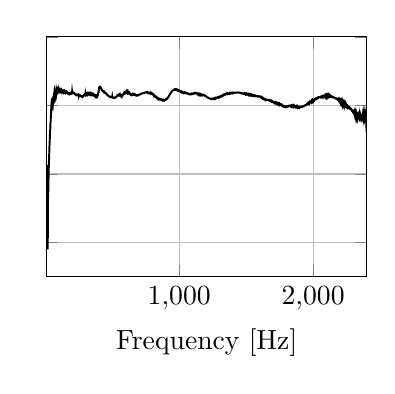
\begin{tikzpicture}

\begin{axis}[%
width=1.6in,
height=1.2in,
at={(1.011in,0.642in)},
scale only axis,
xmin=10,
xmax=2400,
xmajorgrids,
ymin=-30,
ymax=40,
ymajorgrids,
yticklabels={\empty},
xlabel={Frequency [Hz]},
axis background/.style={fill=white}
]
\addplot [color=black,line width=0.7pt,solid,forget plot]
  table[row sep=crcr]{%
0	-7.15873715654256\\
0.666675926054529	10.5087143459122\\
1.33335185210906	12.0967706112481\\
2.00002777816359	6.51246636920068\\
2.66670370421811	-0.175356461979414\\
3.33337963027264	-18.2069665387285\\
4.00005555632717	-15.6498849010992\\
4.6667314823817	-15.9720022096806\\
5.33340740843623	-12.3773277402846\\
6.00008333449076	-11.5127732534421\\
6.66675926054529	-13.124549272927\\
7.33343518659981	-16.8771871920024\\
8.00011111265434	-16.1609324436371\\
8.66678703870887	-16.3957874216142\\
9.3334629647634	-16.1414826002659\\
10.0001388908179	-9.11581854569876\\
10.6668148168725	2.63290680382195\\
11.333490742927	-1.30797727219537\\
12.0001666689815	-17.0636267744369\\
12.666842595036	-6.45026196358668\\
13.3335185210906	2.50663364486626\\
14.0001944471451	-1.70725075474316\\
14.6668703731996	-7.75658468652631\\
15.3335462992542	-9.3483774195719\\
16.0002222253087	-18.6218490262723\\
16.6668981513632	-9.45840899211946\\
17.3335740774177	-13.1140954030332\\
18.0002500034723	-21.9762082832002\\
18.6669259295268	-13.7328495691011\\
19.3336018555813	-11.8237285639594\\
20.0002777816359	-7.07261993440821\\
20.6669537076904	-6.4186096602619\\
21.3336296337449	-6.18112723880758\\
22.0003055597994	-3.42930466318585\\
22.666981485854	-5.04669005883661\\
23.3336574119085	-1.90200540857826\\
24.000333337963	-1.10164436043141\\
24.6670092640176	-0.272686762586023\\
25.3336851900721	1.2811352009495\\
26.0003611161266	2.57386832992159\\
26.6670370421811	2.79701323911136\\
27.3337129682357	3.92461706055076\\
28.0003888942902	4.5923075236652\\
28.6670648203447	5.33513322771373\\
29.3337407463993	6.22858231433341\\
30.0004166724538	6.93789285053402\\
30.6670925985083	7.88093877259057\\
31.3337685245628	8.5797174595324\\
32.0004444506174	9.13987555426015\\
32.6671203766719	9.69391198570301\\
33.3337963027264	10.471697172567\\
34.000472228781	11.2413498429474\\
34.6671481548355	11.9313674436524\\
35.33382408089	12.2206834471294\\
36.0005000069445	12.4355316665065\\
36.6671759329991	12.91188971702\\
37.3338518590536	13.6710847637875\\
38.0005277851081	14.5877480302561\\
38.6672037111627	15.0387885738662\\
39.3338796372172	15.0711002975034\\
40.0005555632717	15.2830740834027\\
40.6672314893262	16.2003603604853\\
41.3339074153808	16.9396542771061\\
42.0005833414353	17.2297836019304\\
42.6672592674898	17.5510274709084\\
43.3339351935444	18.3321890658326\\
44.0006111195989	19.0009998728534\\
44.6672870456534	19.3218972962387\\
45.3339629717079	19.7636726486508\\
46.0006388977625	20.5788804567535\\
46.667314823817	21.0659799329833\\
47.3339907498715	21.0706724489368\\
48.0006666759261	21.2954081888215\\
48.6673426019806	21.7504295307416\\
49.3340185280351	22.0226222784184\\
50.0006944540896	21.2851160722985\\
50.6673703801442	21.2051107463812\\
51.3340463061987	21.2927606988301\\
52.0007222322532	20.8577882479969\\
52.6673981583078	20.6711600742184\\
53.3340740843623	20.9203469279752\\
54.0007500104168	20.8221912113757\\
54.6674259364713	20.6991382976059\\
55.3341018625259	21.0407088483543\\
56.0007777885804	21.1298890830395\\
56.6674537146349	20.9530262480563\\
57.3341296406895	21.3766147555176\\
58.000805566744	21.5208537071508\\
58.6674814927985	21.2653058543976\\
59.334157418853	21.7307748662152\\
60.0008333449076	21.8951668040078\\
60.6675092709621	21.6512975974035\\
61.3341851970166	22.1294978753974\\
62.0008611230712	22.1845098242759\\
62.6675370491257	22.0945317033398\\
63.3342129751802	22.469571046389\\
64.0008889012347	22.4144126743392\\
64.6675648272893	22.4656633253754\\
65.3342407533438	22.7711307278621\\
66.0009166793983	22.595344049128\\
66.6675926054529	22.8211361901548\\
67.3342685315074	22.9714363429243\\
68.0009444575619	22.7483408524739\\
68.6676203836164	23.1900991734327\\
69.334296309671	23.0139565502041\\
70.0009722357255	23.0078941437368\\
70.66764816178	23.2640888008504\\
71.3343240878346	23.0521172453856\\
72.0010000138891	23.2968321488529\\
72.6676759399436	23.2063136781876\\
73.3343518659981	23.3339191542813\\
74.0010277920527	23.4201131005648\\
74.6677037181072	23.2737916065581\\
75.3343796441617	23.6255319273586\\
76.0010555702163	23.3345039510527\\
76.6677314962708	23.6224375724773\\
77.3344074223253	23.6114616424184\\
78.0010833483798	23.656576732508\\
78.6677592744344	23.7364151810855\\
79.3344352004889	23.7429745501262\\
80.0011111265434	23.8351365589793\\
80.667787052598	23.7447631942601\\
81.3344629786525	24.0074055842899\\
82.001138904707	23.8089022197667\\
82.6678148307615	24.0822291816178\\
83.3344907568161	23.9694717725242\\
84.0011666828706	24.1099258580291\\
84.6678426089251	24.0718306679598\\
85.3345185349797	24.2264814415983\\
86.0011944610342	24.1215006110483\\
86.6678703870887	24.2884169849204\\
87.3345463131432	24.2187384264903\\
88.0012222391978	24.3234554885306\\
88.6678981652523	24.3334222819882\\
89.3345740913068	24.3419120374625\\
90.0012500173614	24.3674475386358\\
90.6679259434159	24.4128618208234\\
91.3346018694704	24.3605904365201\\
92.0012777955249	24.490939092038\\
92.6679537215795	24.3883742537234\\
93.334629647634	24.5004186810227\\
94.0013055736885	24.4553094468998\\
94.667981499743	24.5035723715013\\
95.3346574257976	24.4446167778904\\
96.0013333518521	24.5316501403195\\
96.6680092779066	24.4406424070208\\
97.3346852039612	24.5138592854188\\
98.0013611300157	24.4334755790068\\
98.6680370560702	24.4430074171027\\
99.3347129821248	24.4448643874685\\
100.001388908179	24.5830026648291\\
100.668064834234	24.4380232462697\\
101.334740760288	24.367009642005\\
102.001416686343	24.4193073708642\\
102.668092612397	24.3062601108404\\
103.334768538452	24.3793294237293\\
104.001444464506	24.3564597657447\\
104.668120390561	24.3049224218097\\
105.334796316616	24.3674642786709\\
106.00147224267	24.2796963564791\\
106.668148168725	24.3472237616032\\
107.334824094779	24.3024466459277\\
108.001500020834	24.3293347604687\\
108.668175946888	24.3346573062107\\
109.334851872943	24.2937502414376\\
110.001527798997	24.3130074916196\\
110.668203725052	24.3272388220414\\
111.334879651106	24.3171147618053\\
112.001555577161	24.3363629515837\\
112.668231503215	24.3164517932769\\
113.33490742927	24.2788172766694\\
114.001583355324	24.353623658134\\
114.668259281379	24.2556978272775\\
115.334935207433	24.3056736662729\\
116.001611133488	24.2935033143821\\
116.668287059542	24.3115581567028\\
117.334962985597	24.2841837577282\\
118.001638911652	24.3345410688641\\
118.668314837706	24.2299614327879\\
119.334990763761	24.3242644212272\\
120.001666689815	24.2642435178612\\
120.66834261587	24.2865744746116\\
121.335018541924	24.2362265269981\\
122.001694467979	24.2878326149751\\
122.668370394033	24.199568432106\\
123.335046320088	24.2548448168798\\
124.001722246142	24.221737207819\\
124.668398172197	24.2279796362291\\
125.335074098251	24.1628143444844\\
126.001750024306	24.1726631684249\\
126.66842595036	24.1405365714659\\
127.335101876415	24.1014505663823\\
128.001777802469	24.1264812205878\\
128.668453728524	24.0820035236455\\
129.335129654579	24.0995864301708\\
130.001805580633	24.0159117359564\\
130.668481506688	24.0696150031467\\
131.335157432742	23.9974759426067\\
132.001833358797	24.0274658229844\\
132.668509284851	23.9846347041687\\
133.335185210906	24.0053856625507\\
134.00186113696	24.0257414417826\\
134.668537063015	23.9705604936007\\
135.335212989069	24.0116275950592\\
136.001888915124	23.9385430358016\\
136.668564841178	24.003448783508\\
137.335240767233	23.9357430250413\\
138.001916693287	23.9267099430717\\
138.668592619342	23.9397502148012\\
139.335268545396	23.9019035587597\\
140.001944471451	23.9667578531696\\
140.668620397506	23.9002705054755\\
141.33529632356	23.9301926792168\\
142.001972249615	23.9274379783929\\
142.668648175669	23.9107077654991\\
143.335324101724	23.9708240066973\\
144.002000027778	23.8976416979434\\
144.668675953833	23.9280605624893\\
145.335351879887	23.9395178290452\\
146.002027805942	23.9104477198023\\
146.668703731996	24.0042861899005\\
147.335379658051	23.9593716743793\\
148.002055584105	23.9548869966147\\
148.66873151016	23.9741124268126\\
149.335407436214	23.9137084328685\\
150.002083362269	24.0358334053608\\
150.668759288323	24.0129356581571\\
151.335435214378	23.9783044375457\\
152.002111140433	24.0135243729903\\
152.668787066487	23.9570176164768\\
153.335462992542	23.9373671861388\\
154.002138918596	24.0099718833998\\
154.668814844651	23.992175802195\\
155.335490770705	23.9905852435095\\
156.00216669676	24.0154380181123\\
156.668842622814	23.9448424581498\\
157.335518548869	23.9282342359544\\
158.002194474923	23.9412155054648\\
158.668870400978	23.8551568215683\\
159.335546327032	23.8452894749057\\
160.002222253087	23.881183650396\\
160.668898179141	23.8200251691604\\
161.335574105196	23.7885210433908\\
162.00225003125	23.8000977308225\\
162.668925957305	23.7368248711784\\
163.335601883359	23.6809154091656\\
164.002277809414	23.6665957710001\\
164.668953735469	23.6251820323242\\
165.335629661523	23.5786949380226\\
166.002305587578	23.5889468796819\\
166.668981513632	23.5848149862382\\
167.335657439687	23.5652098311667\\
168.002333365741	23.5511967971205\\
168.669009291796	23.5733584242023\\
169.33568521785	23.5538389244039\\
170.002361143905	23.5127478614158\\
170.669037069959	23.5456375024997\\
171.335712996014	23.537627613085\\
172.002388922068	23.4590023938168\\
172.669064848123	23.4686637651834\\
173.335740774177	23.4939816310679\\
174.002416700232	23.4211397740851\\
174.669092626286	23.3974198931325\\
175.335768552341	23.4132330294167\\
176.002444478396	23.4159270564024\\
176.66912040445	23.3919798536214\\
177.335796330505	23.3549185868886\\
178.002472256559	23.409420195141\\
178.669148182614	23.4296019615359\\
179.335824108668	23.3943393217074\\
180.002500034723	23.4064345494135\\
180.669175960777	23.4276710326754\\
181.335851886832	23.4763933629542\\
182.002527812886	23.4551022379621\\
182.669203738941	23.4466717248939\\
183.335879664995	23.4944683083156\\
184.00255559105	23.5051198154288\\
184.669231517104	23.521638340073\\
185.335907443159	23.4895152375784\\
186.002583369213	23.5116009885307\\
186.669259295268	23.5245887945761\\
187.335935221323	23.5634160727353\\
188.002611147377	23.5180171818616\\
188.669287073432	23.5007882491574\\
189.335962999486	23.4703268300687\\
190.002638925541	23.5218474907648\\
190.669314851595	23.5117957925876\\
191.33599077765	23.5073489030819\\
192.002666703704	23.4748867900627\\
192.669342629759	23.5238532127275\\
193.336018555813	23.5443500501714\\
194.002694481868	23.6052564056829\\
194.669370407922	23.6032195687775\\
195.336046333977	23.6067703614072\\
196.002722260031	23.6081462118097\\
196.669398186086	23.6284913263107\\
197.33607411214	23.6683757100492\\
198.002750038195	23.6500605877708\\
198.66942596425	23.6602688200448\\
199.336101890304	23.6430623940489\\
200.002777816359	23.9325844631997\\
200.669453742413	23.7295267431329\\
201.336129668468	23.7453272006813\\
202.002805594522	23.7956790146267\\
202.669481520577	23.7648214347693\\
203.336157446631	23.7392293326182\\
204.002833372686	23.732937791739\\
204.66950929874	23.7163043256602\\
205.336185224795	23.7762496457566\\
206.002861150849	23.8173995548699\\
206.669537076904	23.819690576325\\
207.336213002958	23.8133007788291\\
208.002888929013	23.7553494306647\\
208.669564855067	23.7263702197232\\
209.336240781122	23.7427961208167\\
210.002916707176	23.7457006858622\\
210.669592633231	23.7430014060931\\
211.336268559286	23.7336216256452\\
212.00294448534	23.690354867883\\
212.669620411395	23.664049586363\\
213.336296337449	23.6740149563915\\
214.002972263504	23.6470281106283\\
214.669648189558	23.5774503862567\\
215.336324115613	23.5200440720789\\
216.003000041667	23.501268482812\\
216.669675967722	23.4929198584724\\
217.336351893776	23.484777667757\\
218.003027819831	23.4627902735257\\
218.669703745885	23.4236067287961\\
219.33637967194	23.3896423123424\\
220.003055597994	23.3880062098513\\
220.669731524049	23.360435599666\\
221.336407450103	23.295373972138\\
222.003083376158	23.2435794936051\\
222.669759302213	23.2154136066346\\
223.336435228267	23.1782769365077\\
224.003111154322	23.1475453537114\\
224.669787080376	23.1410471008364\\
225.336463006431	23.1401937937074\\
226.003138932485	23.112688490254\\
226.66981485854	23.0846909271996\\
227.336490784594	23.1030816728332\\
228.003166710649	23.1383110228286\\
228.669842636703	23.0984731681706\\
229.336518562758	23.0754664321036\\
230.003194488812	23.1070024213092\\
230.669870414867	23.1393155792247\\
231.336546340921	23.1138425882487\\
232.003222266976	23.1025528200807\\
232.66989819303	23.0919111899043\\
233.336574119085	23.0269870112512\\
234.00325004514	22.9891308460617\\
234.669925971194	22.9989878077763\\
235.336601897249	23.0044408853645\\
236.003277823303	23.0079139293434\\
236.669953749358	23.053827118727\\
237.336629675412	23.0753116048292\\
238.003305601467	23.0506572130619\\
238.669981527521	23.0938313946732\\
239.336657453576	23.0801118803019\\
240.00333337963	23.0578906249399\\
240.670009305685	23.0979644782169\\
241.336685231739	23.0812668912868\\
242.003361157794	23.0627709669134\\
242.670037083848	23.098894118898\\
243.336713009903	23.0788132473687\\
244.003388935957	23.0869290004178\\
244.670064862012	23.1165807061338\\
245.336740788066	23.0898887826167\\
246.003416714121	23.1126726466507\\
246.670092640176	23.1194517032361\\
247.33676856623	23.0749178994239\\
248.003444492285	23.1072615007923\\
248.670120418339	23.0712759311162\\
249.336796344394	23.0631772802676\\
250.003472270448	22.8922414185675\\
250.670148196503	23.0048298809381\\
251.336824122557	23.0190106554729\\
252.003500048612	22.9874843352767\\
252.670175974666	22.9728118289677\\
253.336851900721	22.982477272407\\
254.003527826775	22.9583179686267\\
254.67020375283	22.9952054740954\\
255.336879678884	22.971121774093\\
256.003555604939	22.9865498886205\\
256.670231530993	22.9807406944549\\
257.336907457048	22.9681666605489\\
258.003583383103	22.9768272202065\\
258.670259309157	22.9192668609388\\
259.336935235212	22.9353555559673\\
260.003611161266	22.8702712699718\\
260.670287087321	22.8697452401716\\
261.336963013375	22.8121830398662\\
262.00363893943	22.81443725079\\
262.670314865484	22.7909267714697\\
263.336990791539	22.7905444968254\\
264.003666717593	22.7798958806609\\
264.670342643648	22.7740146447856\\
265.337018569702	22.7604926592849\\
266.003694495757	22.716614209319\\
266.670370421811	22.7021420662505\\
267.337046347866	22.6644170005054\\
268.00372227392	22.675102369387\\
268.670398199975	22.6585656693192\\
269.33707412603	22.6845816113223\\
270.003750052084	22.6737527254366\\
270.670425978139	22.6463608482636\\
271.337101904193	22.5953795718538\\
272.003777830248	22.5635895606184\\
272.670453756302	22.5674031766485\\
273.337129682357	22.5964060389313\\
274.003805608411	22.6309677360793\\
274.670481534466	22.6240231221093\\
275.33715746052	22.6236841124181\\
276.003833386575	22.5823719455308\\
276.670509312629	22.6111455283201\\
277.337185238684	22.5836961851879\\
278.003861164738	22.6328828994838\\
278.670537090793	22.6388029436635\\
279.337213016847	22.6636737409649\\
280.003888942902	22.6136392098819\\
280.670564868956	22.5802448996619\\
281.337240795011	22.6276271133216\\
282.003916721066	22.6693610695881\\
282.67059264712	22.7209756588301\\
283.337268573175	22.6859101869821\\
284.003944499229	22.7008570077434\\
284.670620425284	22.7234674390024\\
285.337296351338	22.7574004388151\\
286.003972277393	22.8445229709759\\
286.670648203447	22.8422932014905\\
287.337324129502	22.8336215459351\\
288.004000055556	22.8534736044996\\
288.670675981611	22.913823952474\\
289.337351907665	22.9758039708997\\
290.00402783372	22.9447318473799\\
290.670703759774	22.9535210499885\\
291.337379685829	22.9705623129775\\
292.004055611883	23.0256758850494\\
292.670731537938	23.0820633636433\\
293.337407463993	23.0286917736661\\
294.004083390047	23.027952961887\\
294.670759316102	23.1006304178873\\
295.337435242156	23.1056682211187\\
296.004111168211	23.1028400500452\\
296.670787094265	23.081667088508\\
297.33746302032	23.1088261705323\\
298.004138946374	23.1642148879404\\
298.670814872429	23.1531093623504\\
299.337490798483	23.1166864464385\\
300.004166724538	23.3665418070538\\
300.670842650592	23.2281860870225\\
301.337518576647	23.1662682127715\\
302.004194502701	23.1544402143831\\
302.670870428756	23.2342783454354\\
303.33754635481	23.2397236487141\\
304.004222280865	23.2038218162903\\
304.67089820692	23.207616142466\\
305.337574132974	23.2821001817681\\
306.004250059029	23.2330287871902\\
306.670925985083	23.2131033861347\\
307.337601911138	23.2352914154204\\
308.004277837192	23.2795248232929\\
308.670953763247	23.2099013595069\\
309.337629689301	23.2388779697744\\
310.004305615356	23.2800594659038\\
310.67098154141	23.2569280486767\\
311.337657467465	23.2114638342554\\
312.004333393519	23.299609424179\\
312.671009319574	23.2954833083898\\
313.337685245628	23.2558224068988\\
314.004361171683	23.2986141599806\\
314.671037097737	23.3661936285544\\
315.337713023792	23.312169742643\\
316.004388949847	23.3170811893786\\
316.671064875901	23.381741441126\\
317.337740801956	23.3355333422287\\
318.00441672801	23.3836132273774\\
318.671092654065	23.4126914826485\\
319.337768580119	23.3752190931115\\
320.004444506174	23.3986670195967\\
320.671120432228	23.4516374896275\\
321.337796358283	23.4144777344401\\
322.004472284337	23.3988945127971\\
322.671148210392	23.4423603982258\\
323.337824136446	23.4031282824876\\
324.004500062501	23.4396809699807\\
324.671175988555	23.4541101356225\\
325.33785191461	23.3771322764977\\
326.004527840664	23.4192964497452\\
326.671203766719	23.4264931341787\\
327.337879692774	23.3914217573799\\
328.004555618828	23.4557960765174\\
328.671231544883	23.4043099290427\\
329.337907470937	23.3937384344687\\
330.004583396992	23.4275941623696\\
330.671259323046	23.388045098902\\
331.337935249101	23.4432486139232\\
332.004611175155	23.4052667657364\\
332.67128710121	23.400573463867\\
333.337963027264	23.4401434219522\\
334.004638953319	23.357845359059\\
334.671314879373	23.4112267792951\\
335.337990805428	23.4006761429916\\
336.004666731482	23.3773302892184\\
336.671342657537	23.4304678684814\\
337.338018583591	23.3759822922548\\
338.004694509646	23.4198373123268\\
338.671370435701	23.3524395927385\\
339.338046361755	23.3533348287594\\
340.00472228781	23.3711708407037\\
340.671398213864	23.3132864465162\\
341.338074139919	23.3642997499883\\
342.004750065973	23.2957960291322\\
342.671425992028	23.3514068730671\\
343.338101918082	23.3257420257991\\
344.004777844137	23.3174921853021\\
344.671453770191	23.3031464955361\\
345.338129696246	23.263620991949\\
346.0048056223	23.3083246315707\\
346.671481548355	23.2417673165442\\
347.338157474409	23.2851718739417\\
348.004833400464	23.204452393028\\
348.671509326518	23.2326993738068\\
349.338185252573	23.1862953150634\\
350.004861178627	23.2024954774285\\
350.671537104682	23.2016188891564\\
351.338213030737	23.1974198598719\\
352.004888956791	23.1970438821182\\
352.671564882846	23.1711529885069\\
353.3382408089	23.2037763664283\\
354.004916734955	23.1677641995215\\
354.671592661009	23.2069921649515\\
355.338268587064	23.1650070213611\\
356.004944513118	23.1992209603012\\
356.671620439173	23.1409738539685\\
357.338296365227	23.1788912067377\\
358.004972291282	23.1027019847916\\
358.671648217336	23.1476111249839\\
359.338324143391	23.0786920764213\\
360.005000069445	23.1226919519339\\
360.6716759955	23.0611148901713\\
361.338351921554	23.092286326067\\
362.005027847609	23.0470916754452\\
362.671703773664	23.0664222074796\\
363.338379699718	23.0238804328784\\
364.005055625773	23.035169672148\\
364.671731551827	23.0093452500552\\
365.338407477882	22.9938314216959\\
366.005083403936	22.9830093396502\\
366.671759329991	22.950682957497\\
367.338435256045	22.9652681177984\\
368.0051111821	22.9115777998351\\
368.671787108154	22.9378777062769\\
369.338463034209	22.8725537469231\\
370.005138960263	22.9078087983924\\
370.671814886318	22.8444563514053\\
371.338490812372	22.8702265014038\\
372.005166738427	22.823562456798\\
372.671842664481	22.8208599571976\\
373.338518590536	22.8111223570435\\
374.005194516591	22.7522474525364\\
374.671870442645	22.7817476427405\\
375.3385463687	22.6941969850737\\
376.005222294754	22.7383231711478\\
376.671898220809	22.6754846835769\\
377.338574146863	22.6877581861511\\
378.005250072918	22.6906717089616\\
378.671925998972	22.658351924489\\
379.338601925027	22.705607335846\\
380.005277851081	22.6429832893611\\
380.671953777136	22.6691583584912\\
381.33862970319	22.6194392027024\\
382.005305629245	22.5757695192077\\
382.671981555299	22.5905242397834\\
383.338657481354	22.5197369972299\\
384.005333407408	22.5456802402232\\
384.672009333463	22.5340064505076\\
385.338685259517	22.5096147354606\\
386.005361185572	22.5682871856995\\
386.672037111627	22.5213255359728\\
387.338713037681	22.5711912354341\\
388.005388963736	22.625259679459\\
388.67206488979	22.6288198538351\\
389.338740815845	22.7603325712579\\
390.005416741899	22.8129192557627\\
390.672092667954	22.8784920405188\\
391.338768594008	23.0206437879727\\
392.005444520063	23.0769470015594\\
392.672120446117	23.2209934474768\\
393.338796372172	23.3752791549899\\
394.005472298226	23.4317600457901\\
394.672148224281	23.5820447454569\\
395.338824150335	23.7302811865809\\
396.00550007639	23.8240416597948\\
396.672176002444	24.0128021996323\\
397.338851928499	24.1482868134601\\
398.005527854554	24.2360199546688\\
398.672203780608	24.4474335771642\\
399.338879706663	24.6038826762412\\
400.005555632717	24.5605666726398\\
400.672231558772	24.8100488703285\\
401.338907484826	24.9634337837249\\
402.005583410881	25.0224017171142\\
402.672259336935	25.1189085776965\\
403.33893526299	25.235563413276\\
404.005611189044	25.2717036553352\\
404.672287115099	25.3314128075437\\
405.338963041153	25.3991343019002\\
406.005638967208	25.3935888823572\\
406.672314893262	25.3965680663757\\
407.338990819317	25.4356907615614\\
408.005666745371	25.4272133150631\\
408.672342671426	25.366634698988\\
409.339018597481	25.3729685396194\\
410.005694523535	25.3840453400317\\
410.67237044959	25.2965949046627\\
411.339046375644	25.2510525177916\\
412.005722301699	25.2758580500552\\
412.672398227753	25.2077616573045\\
413.339074153808	25.1164201027822\\
414.005750079862	25.1016445456299\\
414.672426005917	25.058259510491\\
415.339101931971	24.9882349890131\\
416.005777858026	24.9181123919607\\
416.67245378408	24.8757656863904\\
417.339129710135	24.8858751028074\\
418.005805636189	24.8112830993537\\
418.672481562244	24.7362554872007\\
419.339157488298	24.7263307536006\\
420.005833414353	24.7389744979165\\
420.672509340407	24.6800214622345\\
421.339185266462	24.5843610206647\\
422.005861192517	24.6022249994799\\
422.672537118571	24.5761496535907\\
423.339213044626	24.5646465042338\\
424.00588897068	24.4752897618484\\
424.672564896735	24.4285861432201\\
425.339240822789	24.4314731468244\\
426.005916748844	24.3979437025808\\
426.672592674898	24.3015094891424\\
427.339268600953	24.2545541748938\\
428.005944527007	24.2328455773834\\
428.672620453062	24.2737375769304\\
429.339296379116	24.2632491902619\\
430.005972305171	24.2057651955647\\
430.672648231225	24.1714503299811\\
431.33932415728	24.1623235443258\\
432.006000083334	24.1842873641646\\
432.672676009389	24.1828452161925\\
433.339351935444	24.1055814305408\\
434.006027861498	24.09285264821\\
434.672703787553	24.047628526424\\
435.339379713607	24.0911791492153\\
436.006055639662	24.0617381755948\\
436.672731565716	24.0487885524772\\
437.339407491771	23.9880694116177\\
438.006083417825	23.9276842342827\\
438.67275934388	23.9472251782106\\
439.339435269934	23.9199627050903\\
440.006111195989	23.9538873760375\\
440.672787122043	23.892317954538\\
441.339463048098	23.8535029673726\\
442.006138974152	23.813718178514\\
442.672814900207	23.7912046507748\\
443.339490826261	23.8011827237526\\
444.006166752316	23.8067842569663\\
444.672842678371	23.7821685741767\\
445.339518604425	23.7650070458023\\
446.00619453048	23.7125347109658\\
446.672870456534	23.6612109064161\\
447.339546382589	23.6582383057953\\
448.006222308643	23.6397043370453\\
448.672898234698	23.6398786909826\\
449.339574160752	23.6475041293184\\
450.006250086807	23.6220633837197\\
450.672926012861	23.5705148100686\\
451.339601938916	23.5441797931312\\
452.00627786497	23.4955456219766\\
452.672953791025	23.4503897931678\\
453.339629717079	23.4563352286849\\
454.006305643134	23.4331579273573\\
454.672981569188	23.425576157168\\
455.339657495243	23.4023542595\\
456.006333421298	23.4164633563494\\
456.673009347352	23.3596926012022\\
457.339685273407	23.329539130947\\
458.006361199461	23.282100168342\\
458.673037125516	23.2645172262514\\
459.33971305157	23.211896289963\\
460.006388977625	23.1642517273922\\
460.673064903679	23.1451054452469\\
461.339740829734	23.1215301660216\\
462.006416755788	23.1271164476067\\
462.673092681843	23.0785693515525\\
463.339768607897	23.0677163935001\\
464.006444533952	23.0535931639354\\
464.673120460006	23.0373979010306\\
465.339796386061	23.0214724946777\\
466.006472312115	22.9684360172689\\
466.67314823817	22.9492822646665\\
467.339824164225	22.9205703994463\\
468.006500090279	22.8892631135468\\
468.673176016334	22.8842417485463\\
469.339851942388	22.8362122012308\\
470.006527868443	22.8121458874946\\
470.673203794497	22.7881002412262\\
471.339879720552	22.7517999758853\\
472.006555646606	22.7575020839074\\
472.673231572661	22.7344592916752\\
473.339907498715	22.7201364600742\\
474.00658342477	22.7110151487217\\
474.673259350824	22.6790260133921\\
475.339935276879	22.6566296224347\\
476.006611202933	22.6398455086865\\
476.673287128988	22.6107385911572\\
477.339963055042	22.5921911313787\\
478.006638981097	22.5889108793928\\
478.673314907152	22.5665846391812\\
479.339990833206	22.5654983876713\\
480.006666759261	22.5764465071147\\
480.673342685315	22.5512033056028\\
481.34001861137	22.5359062912685\\
482.006694537424	22.5332557232302\\
482.673370463479	22.5096901998091\\
483.340046389533	22.4847600438032\\
484.006722315588	22.4827123785872\\
484.673398241642	22.4748141311656\\
485.340074167697	22.4535139679094\\
486.006750093751	22.4558405256336\\
486.673426019806	22.4576923512691\\
487.34010194586	22.4480277084016\\
488.006777871915	22.452118245327\\
488.673453797969	22.4723476677798\\
489.340129724024	22.4790314240742\\
490.006805650078	22.4701324928377\\
490.673481576133	22.4710256311865\\
491.340157502188	22.4746986008659\\
492.006833428242	22.458796802072\\
492.673509354297	22.436710203806\\
493.340185280351	22.4285228065914\\
494.006861206406	22.42974129422\\
494.67353713246	22.4146014883439\\
495.340213058515	22.3918596302885\\
496.006888984569	22.3873433462568\\
496.673564910624	22.4011294188386\\
497.340240836678	22.3993600031334\\
498.006916762733	22.3934189857785\\
498.673592688787	22.3959247581123\\
499.340268614842	22.3980804467826\\
500.006944540896	22.5556762884854\\
500.673620466951	22.3974492753894\\
501.340296393005	22.368857290977\\
502.00697231906	22.3462530764068\\
502.673648245115	22.3367616084347\\
503.340324171169	22.3236330454825\\
504.007000097224	22.3130497843336\\
504.673676023278	22.3087159923272\\
505.340351949333	22.3151007138196\\
506.007027875387	22.3309347341289\\
506.673703801442	22.3260035011254\\
507.340379727496	22.3026852159121\\
508.007055653551	22.2700563983849\\
508.673731579605	22.2289702448306\\
509.34040750566	22.227819946724\\
510.007083431714	22.2524631932524\\
510.673759357769	22.2852562256613\\
511.340435283823	22.2885169498584\\
512.007111209878	22.2530696843343\\
512.673787135932	22.2161262023443\\
513.340463061987	22.1976125470916\\
514.007138988041	22.222057758885\\
514.673814914096	22.2408173670611\\
515.340490840151	22.2532140444528\\
516.007166766205	22.255704132218\\
516.67384269226	22.2528469180602\\
517.340518618314	22.2412670775663\\
518.007194544369	22.2302604231504\\
518.673870470423	22.2580699907529\\
519.340546396478	22.2960580258133\\
520.007222322532	22.3215956694387\\
520.673898248587	22.292711184102\\
521.340574174641	22.2921542442947\\
522.007250100696	22.3191795064228\\
522.67392602675	22.3555140919138\\
523.340601952805	22.364265945962\\
524.007277878859	22.3797601749284\\
524.673953804914	22.3714415496905\\
525.340629730968	22.3680027167281\\
526.007305657023	22.4088621026103\\
526.673981583078	22.4640973821973\\
527.340657509132	22.4601723889253\\
528.007333435187	22.4487260807839\\
528.674009361241	22.4783243839663\\
529.340685287296	22.5159768553421\\
530.00736121335	22.5684477666636\\
530.674037139405	22.578746650228\\
531.340713065459	22.5672010872706\\
532.007388991514	22.613410184191\\
532.674064917568	22.6720092349587\\
533.340740843623	22.6848708485002\\
534.007416769677	22.7004009522696\\
534.674092695732	22.7033647144998\\
535.340768621786	22.7570213247332\\
536.007444547841	22.8066157979055\\
536.674120473896	22.7771235107182\\
537.34079639995	22.8103882371864\\
538.007472326005	22.8508287683496\\
538.674148252059	22.8809487827767\\
539.340824178114	22.8822835892378\\
540.007500104168	22.872836926273\\
540.674176030223	22.9409284225212\\
541.340851956277	22.9486301332984\\
542.007527882332	22.9503051462533\\
542.674203808386	22.9440067977203\\
543.340879734441	23.0121243840464\\
544.007555660495	23.0034512520761\\
544.67423158655	22.9891208696874\\
545.340907512604	23.010790639817\\
546.007583438659	23.0600250441806\\
546.674259364713	23.0299195345168\\
547.340935290768	23.0281484988089\\
548.007611216823	23.0740637133528\\
548.674287142877	23.076494011509\\
549.340963068932	23.0433162692488\\
550.007638994986	23.0889741013555\\
550.674314921041	23.1153192163153\\
551.340990847095	23.0904431790381\\
552.00766677315	23.0948912368854\\
552.674342699204	23.1411827306395\\
553.341018625259	23.0798824324349\\
554.007694551313	23.0976578046195\\
554.674370477368	23.1022173080237\\
555.341046403422	23.0775136151027\\
556.007722329477	23.0423404850017\\
556.674398255531	23.0845663505847\\
557.341074181586	23.0514846409615\\
558.00775010764	23.0222442900952\\
558.674426033695	23.0781988252938\\
559.341101959749	23.0016519343541\\
560.007777885804	22.9867363234617\\
560.674453811858	22.9995238939942\\
561.341129737913	22.9182260060531\\
562.007805663968	22.9071470208661\\
562.674481590022	22.8978954225745\\
563.341157516077	22.8276167423139\\
564.007833442131	22.8319379404363\\
564.674509368186	22.7980293203263\\
565.34118529424	22.7236366916712\\
566.007861220295	22.7328069820359\\
566.674537146349	22.6729735942675\\
567.341213072404	22.6476000823122\\
568.007888998458	22.6909341331093\\
568.674564924513	22.6183503679082\\
569.341240850567	22.6432736310698\\
570.007916776622	22.6595463287102\\
570.674592702676	22.6097747623807\\
571.341268628731	22.6929377403755\\
572.007944554785	22.7009934548951\\
572.67462048084	22.7021026774696\\
573.341296406895	22.7551728416182\\
574.007972332949	22.7505180240948\\
574.674648259004	22.8222548355523\\
575.341324185058	22.8412596694343\\
576.008000111113	22.8731501858362\\
576.674676037167	22.9496451050659\\
577.341351963222	22.9433182519649\\
578.008027889276	23.0342522269302\\
578.674703815331	23.0519341435632\\
579.341379741385	23.1121322335299\\
580.00805566744	23.1400469619068\\
580.674731593494	23.1552000982357\\
581.341407519549	23.2507566754524\\
582.008083445603	23.2489658838062\\
582.674759371658	23.3347560867854\\
583.341435297712	23.3344325894672\\
584.008111223767	23.4044509373415\\
584.674787149822	23.4331699427611\\
585.341463075876	23.4618953372666\\
586.008139001931	23.5328919450315\\
586.674814927985	23.5284988425091\\
587.34149085404	23.5757448014353\\
588.008166780094	23.5550104373674\\
588.674842706149	23.6571778406404\\
589.341518632203	23.6381512968117\\
590.008194558258	23.6965635088613\\
590.674870484312	23.6916376623203\\
591.341546410367	23.7451371180211\\
592.008222336421	23.7191740388327\\
592.674898262476	23.7718895764984\\
593.34157418853	23.8017976003933\\
594.008250114585	23.8229117895531\\
594.674926040639	23.8386868529616\\
595.341601966694	23.8782268859547\\
596.008277892749	23.8810183635803\\
596.674953818803	23.8756709635537\\
597.341629744858	23.9056998399092\\
598.008305670912	23.9031421113195\\
598.674981596967	23.9181515628447\\
599.341657523021	23.9508634240059\\
600.008333449076	23.8805873602388\\
600.67500937513	23.9622586843332\\
601.341685301185	23.9889985800693\\
602.008361227239	24.0026376782776\\
602.675037153294	23.9904799879627\\
603.341713079348	24.0386198925986\\
604.008389005403	23.9880625043385\\
604.675064931457	24.0611437363596\\
605.341740857512	24.0076429547272\\
606.008416783566	24.0519202565057\\
606.675092709621	24.0169048599477\\
607.341768635676	24.0588644656048\\
608.00844456173	24.0125309286435\\
608.675120487785	24.066765564531\\
609.341796413839	24.0119546403279\\
610.008472339894	24.0349107153302\\
610.675148265948	24.0239681379336\\
611.341824192003	23.9930567324848\\
612.008500118057	24.0367278043696\\
612.675176044112	23.9427825836015\\
613.341851970166	24.0136383106808\\
614.008527896221	23.9260728870395\\
614.675203822275	23.967874560845\\
615.34187974833	23.9386309128271\\
616.008555674384	23.9121841921643\\
616.675231600439	23.9527786815655\\
617.341907526493	23.8708946197959\\
618.008583452548	23.9409060531761\\
618.675259378603	23.869758995315\\
619.341935304657	23.8912419070363\\
620.008611230711	23.8831161386137\\
620.675287156766	23.8208071598346\\
621.341963082821	23.8456012404703\\
622.008639008875	23.7799195903703\\
622.67531493493	23.7539739552072\\
623.341990860984	23.7712922896337\\
624.008666787039	23.7059846392007\\
624.675342713093	23.736307461616\\
625.342018639148	23.7057318597623\\
626.008694565202	23.6457567355793\\
626.675370491257	23.6704860752896\\
627.342046417311	23.5846152449446\\
628.008722343366	23.5929820263484\\
628.67539826942	23.5927149191422\\
629.342074195475	23.534178373717\\
630.008750121529	23.5378234635832\\
630.675426047584	23.4899142794554\\
631.342101973638	23.4418013879416\\
632.008777899693	23.4648643283008\\
632.675453825748	23.4200253179656\\
633.342129751802	23.3738336644112\\
634.008805677857	23.3746893631768\\
634.675481603911	23.3017077656367\\
635.342157529966	23.3145078132275\\
636.00883345602	23.2782471960621\\
636.675509382075	23.2271912459278\\
637.342185308129	23.1865933222311\\
638.008861234184	23.2035485789039\\
638.675537160238	23.1457123345192\\
639.342213086293	23.1202529941746\\
640.008889012347	23.1266392408424\\
640.675564938402	23.0712377604073\\
641.342240864456	23.0985516195479\\
642.008916790511	23.0707215012686\\
642.675592716565	23.0583808867183\\
643.34226864262	23.0722746298861\\
644.008944568675	23.0757854678728\\
644.675620494729	23.0775737190015\\
645.342296420784	23.0655170251614\\
646.008972346838	23.1075933430503\\
646.675648272893	23.1032873247139\\
647.342324198947	23.0881326919386\\
648.009000125002	23.1283171868152\\
648.675676051056	23.1461635053042\\
649.342351977111	23.1451561411158\\
650.009027903165	23.1274044321186\\
650.67570382922	23.174074062497\\
651.342379755274	23.2165995015894\\
652.009055681329	23.1523605789994\\
652.675731607383	23.1796478983035\\
653.342407533438	23.2426741944987\\
654.009083459492	23.1942652917014\\
654.675759385547	23.1872648005046\\
655.342435311602	23.2039010623998\\
656.009111237656	23.2250070747326\\
656.675787163711	23.2131701195773\\
657.342463089765	23.1764770776587\\
658.00913901582	23.2067951136444\\
658.675814941874	23.2103111549554\\
659.342490867929	23.2263659548199\\
660.009166793983	23.1517168329694\\
660.675842720038	23.1637425728063\\
661.342518646092	23.2204451817756\\
662.009194572147	23.1850833790367\\
662.675870498201	23.1417722565883\\
663.342546424256	23.1340666490165\\
664.00922235031	23.1814717589597\\
664.675898276365	23.1479593637174\\
665.342574202419	23.1414817988859\\
666.009250128474	23.1011237830234\\
666.675926054529	23.1083220487726\\
667.342601980583	23.1116942065265\\
668.009277906638	23.1384149423654\\
668.675953832692	23.0763671735842\\
669.342629758747	23.0473479102096\\
670.009305684801	23.0466727826005\\
670.675981610856	23.1066009084499\\
671.34265753691	23.0605356569891\\
672.009333462965	23.0274246531842\\
672.676009389019	22.9986773913877\\
673.342685315074	23.0164546496092\\
674.009361241128	23.0306657792978\\
674.676037167183	23.015501261291\\
675.342713093237	23.0101616378404\\
676.009389019292	22.9644256087\\
676.676064945346	22.9727508843167\\
677.342740871401	22.9493790455104\\
678.009416797456	22.9720288308553\\
678.67609272351	22.9863316519141\\
679.342768649565	22.9663997270916\\
680.009444575619	22.9487900422614\\
680.676120501674	22.9024513546758\\
681.342796427728	22.9107880874405\\
682.009472353783	22.9512499995849\\
682.676148279837	22.9612981646361\\
683.342824205892	22.9696963441367\\
684.009500131946	22.9278079765716\\
684.676176058001	22.8881528900286\\
685.342851984055	22.9077360090166\\
686.00952791011	22.9132862841628\\
686.676203836164	22.9225816221733\\
687.342879762219	22.9567514469161\\
688.009555688273	22.939182938288\\
688.676231614328	22.9343930613014\\
689.342907540382	22.9485481762084\\
690.009583466437	22.9323852669615\\
690.676259392492	22.9236160133126\\
691.342935318546	22.9385515667977\\
692.009611244601	22.9460275375806\\
692.676287170655	22.9449960614785\\
693.34296309671	22.9775047277762\\
694.009639022764	23.0168108491432\\
694.676314948819	23.0147278233748\\
695.342990874873	23.0151084387104\\
696.009666800928	23.0314915693083\\
696.676342726982	23.0319153938354\\
697.343018653037	23.0092193284002\\
698.009694579091	23.0079175857448\\
698.676370505146	23.0389134326495\\
699.3430464312	23.0635381375235\\
700.009722357255	23.0806113725207\\
700.676398283309	23.1070747387522\\
701.343074209364	23.1429198483529\\
702.009750135419	23.1821318274822\\
702.676426061473	23.2034371400095\\
703.343101987528	23.1972361966381\\
704.009777913582	23.2023769448256\\
704.676453839637	23.2129795901655\\
705.343129765691	23.2377456291667\\
706.009805691746	23.2388210269578\\
706.6764816178	23.2402446979098\\
707.343157543855	23.2436202256167\\
708.009833469909	23.2531139776697\\
708.676509395964	23.2677796546635\\
709.343185322018	23.2950853772041\\
710.009861248073	23.3161448556964\\
710.676537174127	23.3230767972559\\
711.343213100182	23.3224069034599\\
712.009889026236	23.3363894122506\\
712.676564952291	23.352376178701\\
713.343240878346	23.3746584756115\\
714.0099168044	23.3897376175182\\
714.676592730455	23.4187604304551\\
715.343268656509	23.4314457069027\\
716.009944582564	23.4470768869404\\
716.676620508618	23.4473138841561\\
717.343296434673	23.4513154347126\\
718.009972360727	23.4618164961054\\
718.676648286782	23.4664520548425\\
719.343324212836	23.48092191548\\
720.010000138891	23.4868694976053\\
720.676676064945	23.4959092099804\\
721.343351991	23.5049851450233\\
722.010027917054	23.5152913741979\\
722.676703843109	23.5305386459897\\
723.343379769163	23.5348326469472\\
724.010055695218	23.5445654417811\\
724.676731621273	23.5504991007689\\
725.343407547327	23.5531631573508\\
726.010083473382	23.5690583822292\\
726.676759399436	23.5758723707306\\
727.343435325491	23.5926090661921\\
728.010111251545	23.6072628360651\\
728.6767871776	23.623601748347\\
729.343463103654	23.6329335257597\\
730.010139029709	23.6459222342708\\
730.676814955763	23.6525980284254\\
731.343490881818	23.6563295422292\\
732.010166807872	23.6524490742021\\
732.676842733927	23.647184839444\\
733.343518659981	23.633493465175\\
734.010194586036	23.622250891434\\
734.67687051209	23.6159784217895\\
735.343546438145	23.6190783694874\\
736.0102223642	23.6297958549446\\
736.676898290254	23.6526501551071\\
737.343574216309	23.6853001046733\\
738.010250142363	23.701724678475\\
738.676926068418	23.7203608777794\\
739.343601994472	23.7284602507321\\
740.010277920527	23.7187965816374\\
740.676953846581	23.7005295945607\\
741.343629772636	23.6926600441393\\
742.01030569869	23.6987851950776\\
742.676981624745	23.7149946195021\\
743.343657550799	23.7384591069874\\
744.010333476854	23.7561098397947\\
744.677009402908	23.7656183213648\\
745.343685328963	23.7724211810449\\
746.010361255017	23.7724226398048\\
746.677037181072	23.7798018559281\\
747.343713107127	23.7845976103599\\
748.010389033181	23.7807200609043\\
748.677064959236	23.7749101452311\\
749.34374088529	23.7741154810056\\
750.010416811345	23.796634395869\\
750.677092737399	23.8309667702415\\
751.343768663454	23.8433429958031\\
752.010444589508	23.8211403942757\\
752.677120515563	23.7865258034788\\
753.343796441617	23.7785537748694\\
754.010472367672	23.8137078229705\\
754.677148293726	23.8580048500374\\
755.343824219781	23.8458546378775\\
756.010500145835	23.8099426211288\\
756.67717607189	23.8030231652679\\
757.343851997944	23.8245262660432\\
758.010527923999	23.8210469904165\\
758.677203850054	23.8140119044577\\
759.343879776108	23.8294331705672\\
760.010555702162	23.8467926262879\\
760.677231628217	23.8025592074172\\
761.343907554272	23.7703411426533\\
762.010583480326	23.8015819343721\\
762.677259406381	23.8354867147965\\
763.343935332435	23.8077505483757\\
764.01061125849	23.7721403159768\\
764.677287184544	23.7745036805367\\
765.343963110599	23.7911545262541\\
766.010639036653	23.8057779241814\\
766.677314962708	23.7873733000585\\
767.343990888762	23.7461609218968\\
768.010666814817	23.753132996585\\
768.677342740871	23.7736846193395\\
769.344018666926	23.7601698551631\\
770.01069459298	23.7618074665837\\
770.677370519035	23.7302630308509\\
771.344046445089	23.7042278043597\\
772.010722371144	23.7574223447078\\
772.677398297199	23.7487646456219\\
773.344074223253	23.6839789911615\\
774.010750149308	23.7089975063742\\
774.677426075362	23.7273710275949\\
775.344102001417	23.7155070618461\\
776.010777927471	23.6884144581687\\
776.677453853526	23.6816103531152\\
777.34412977958	23.707294241114\\
778.010805705635	23.6926215517277\\
778.677481631689	23.6866564038993\\
779.344157557744	23.6474536777702\\
780.010833483798	23.6946382443034\\
780.677509409853	23.6978930964141\\
781.344185335907	23.6335629969068\\
782.010861261962	23.6634253692965\\
782.677537188016	23.6684351830178\\
783.344213114071	23.6543849525892\\
784.010889040126	23.6321139751109\\
784.67756496618	23.6586669126238\\
785.344240892235	23.6377648414625\\
786.010916818289	23.6430628515877\\
786.677592744344	23.5962724813471\\
787.344268670398	23.6591462122314\\
788.010944596453	23.5986072018452\\
788.677620522507	23.5932668974924\\
789.344296448562	23.6056921710213\\
790.010972374616	23.594592645914\\
790.677648300671	23.5589758714033\\
791.344324226725	23.578499149603\\
792.01100015278	23.5619152783938\\
792.677676078834	23.5371886993653\\
793.344352004889	23.5175638743205\\
794.011027930943	23.5410699929958\\
794.677703856998	23.4847255499225\\
795.344379783053	23.4762598301396\\
796.011055709107	23.5007746126234\\
796.677731635162	23.4334251169915\\
797.344407561216	23.4406835334558\\
798.011083487271	23.423551780872\\
798.677759413325	23.3836615258482\\
799.34443533938	23.3712116964328\\
800.011111265434	23.3464470775564\\
800.677787191489	23.3123855994777\\
801.344463117543	23.330251517603\\
802.011139043598	23.2740297828944\\
802.677814969652	23.2650722911698\\
803.344490895707	23.232593118773\\
804.011166821761	23.2270389770053\\
804.677842747816	23.1822096779909\\
805.34451867387	23.1771461965789\\
806.011194599925	23.1282878184583\\
806.67787052598	23.1238834650183\\
807.344546452034	23.0902544246641\\
808.011222378089	23.0570561101117\\
808.677898304143	23.0466976640198\\
809.344574230198	23.0298038025368\\
810.011250156252	22.9588441094959\\
810.677926082307	23.0018697553262\\
811.344602008361	22.936597138072\\
812.011277934416	22.9259417004265\\
812.67795386047	22.9100470182289\\
813.344629786525	22.8835386128617\\
814.011305712579	22.8558248487175\\
814.677981638634	22.833480860987\\
815.344657564688	22.8180939307043\\
816.011333490743	22.8135784254726\\
816.678009416797	22.7463410111136\\
817.344685342852	22.7610203829671\\
818.011361268907	22.7322922194165\\
818.678037194961	22.7188892031191\\
819.344713121016	22.7025841491073\\
820.01138904707	22.6442547833458\\
820.678064973125	22.6752305102308\\
821.344740899179	22.6301203342746\\
822.011416825234	22.6346224297041\\
822.678092751288	22.5772283453905\\
823.344768677343	22.5661822918427\\
824.011444603397	22.5605695533062\\
824.678120529452	22.5439826769726\\
825.344796455506	22.5184558752568\\
826.011472381561	22.4916776544438\\
826.678148307615	22.4661267185983\\
827.34482423367	22.4357930121631\\
828.011500159724	22.4503824207671\\
828.678176085779	22.397339954099\\
829.344852011833	22.4158834114791\\
830.011527937888	22.3319052618051\\
830.678203863943	22.3448836532995\\
831.344879789997	22.2925004629504\\
832.011555716052	22.2871201245659\\
832.678231642106	22.254574550138\\
833.344907568161	22.2678164347568\\
834.011583494215	22.2094249817561\\
834.67825942027	22.2209623225987\\
835.344935346324	22.1716725844095\\
836.011611272379	22.1579734071428\\
836.678287198433	22.1250104460861\\
837.344963124488	22.1162106211392\\
838.011639050542	22.0759210373798\\
838.678314976597	22.0920289821163\\
839.344990902651	22.0415325424152\\
840.011666828706	22.0379083196923\\
840.67834275476	22.0126529796581\\
841.345018680815	22.0354222971823\\
842.01169460687	21.9657744513101\\
842.678370532924	21.9950627024183\\
843.345046458979	21.959362056018\\
844.011722385033	21.9539106245945\\
844.678398311088	21.9127198983184\\
845.345074237142	21.9525727640256\\
846.011750163197	21.909164958997\\
846.678426089251	21.8993191942726\\
847.345102015306	21.8932463793399\\
848.01177794136	21.886800682874\\
848.678453867415	21.8777113216721\\
849.345129793469	21.8454854133775\\
850.011805719524	21.8744706843142\\
850.678481645578	21.8400531616394\\
851.345157571633	21.8574032707273\\
852.011833497687	21.8063399602622\\
852.678509423742	21.8291707988836\\
853.345185349797	21.8257764326659\\
854.011861275851	21.7920142319313\\
854.678537201906	21.7928114019926\\
855.34521312796	21.7752680482553\\
856.011889054015	21.8102587561136\\
856.678564980069	21.7767600698792\\
857.345240906124	21.7843125355645\\
858.011916832178	21.7897629958131\\
858.678592758233	21.781905592999\\
859.345268684287	21.8035182433575\\
860.011944610342	21.7503954752272\\
860.678620536396	21.7480540067359\\
861.345296462451	21.7415960650876\\
862.011972388505	21.7212121050725\\
862.67864831456	21.749083622938\\
863.345324240614	21.7141188451205\\
864.012000166669	21.7202243529592\\
864.678676092724	21.7154410623752\\
865.345352018778	21.6783093078939\\
866.012027944833	21.7017993120571\\
866.678703870887	21.6723481207449\\
867.345379796942	21.6566507884827\\
868.012055722996	21.6795393051187\\
868.678731649051	21.6347461431731\\
869.345407575105	21.6315565589786\\
870.01208350116	21.6392495452065\\
870.678759427214	21.614280067601\\
871.345435353269	21.6464405978681\\
872.012111279323	21.6237430638077\\
872.678787205378	21.5647319128906\\
873.345463131432	21.5826831368792\\
874.012139057487	21.5882032792836\\
874.678814983541	21.5773477270498\\
875.345490909596	21.593680803421\\
876.012166835651	21.563401697428\\
876.678842761705	21.5531643714124\\
877.34551868776	21.5765163789445\\
878.012194613814	21.5545320706207\\
878.678870539869	21.508288417968\\
879.345546465923	21.5498812009246\\
880.012222391978	21.5508132863589\\
880.678898318032	21.5147545437381\\
881.345574244087	21.5404085172841\\
882.012250170141	21.5761681482087\\
882.678926096196	21.5328328401813\\
883.34560202225	21.5403201255586\\
884.012277948305	21.5774516174571\\
884.678953874359	21.5446492409024\\
885.345629800414	21.5214067170058\\
886.012305726468	21.568381277268\\
886.678981652523	21.5582926654186\\
887.345657578578	21.5245749775924\\
888.012333504632	21.5687494403617\\
888.679009430687	21.5763740500678\\
889.345685356741	21.5445564244656\\
890.012361282796	21.5770259220888\\
890.67903720885	21.5924344238192\\
891.345713134905	21.591049981083\\
892.012389060959	21.5847696890082\\
892.679064987014	21.5914002202303\\
893.345740913068	21.6267422328808\\
894.012416839123	21.6236499848409\\
894.679092765177	21.6103529758651\\
895.345768691232	21.6457718459671\\
896.012444617286	21.6602353657822\\
896.679120543341	21.6617842155454\\
897.345796469395	21.6532574688718\\
898.01247239545	21.6770009716539\\
898.679148321504	21.7234366548891\\
899.345824247559	21.7010498376848\\
900.012500173613	21.6935042041642\\
900.679176099668	21.7212166697007\\
901.345852025723	21.7760315091477\\
902.012527951777	21.7748452027565\\
902.679203877832	21.7817350053831\\
903.345879803886	21.7924738048583\\
904.012555729941	21.8348492709104\\
904.679231655995	21.8564750859\\
905.34590758205	21.8660910496602\\
906.012583508104	21.8705077703193\\
906.679259434159	21.9037522513475\\
907.345935360213	21.9494467052829\\
908.012611286268	21.9928283132141\\
908.679287212322	21.9975600231928\\
909.345963138377	22.0191063476531\\
910.012639064431	22.0456857305327\\
910.679314990486	22.1016801456314\\
911.34599091654	22.1173822053652\\
912.012666842595	22.1445521461763\\
912.67934276865	22.1347443194722\\
913.346018694704	22.1858045676258\\
914.012694620759	22.2101527156677\\
914.679370546813	22.2751835198286\\
915.346046472868	22.3193304201988\\
916.012722398922	22.3327929131323\\
916.679398324977	22.3850078651014\\
917.346074251031	22.3897869317004\\
918.012750177086	22.4600814758659\\
918.67942610314	22.4925894131589\\
919.346102029195	22.5234268441138\\
920.012777955249	22.5698865144314\\
920.679453881304	22.5924000490605\\
921.346129807358	22.6526245511415\\
922.012805733413	22.7088826307128\\
922.679481659467	22.7417421025648\\
923.346157585522	22.802833481229\\
924.012833511577	22.8242587839818\\
924.679509437631	22.8643774587498\\
925.346185363686	22.9206038729767\\
926.01286128974	22.9552323534503\\
926.679537215795	22.9909762710224\\
927.346213141849	23.0582506070459\\
928.012889067904	23.0944683718885\\
928.679564993958	23.142439532014\\
929.346240920013	23.2099693424213\\
930.012916846067	23.2491488401517\\
930.679592772122	23.2576291675653\\
931.346268698176	23.2979576862761\\
932.012944624231	23.3431067554339\\
932.679620550285	23.3856348281568\\
933.34629647634	23.4484277106392\\
934.012972402394	23.5031449956164\\
934.679648328449	23.5308505186907\\
935.346324254504	23.5652804033016\\
936.013000180558	23.6332746499125\\
936.679676106613	23.6804375262843\\
937.346352032667	23.6905779861082\\
938.013027958722	23.7024347967036\\
938.679703884776	23.7570073631558\\
939.346379810831	23.8117806859368\\
940.013055736885	23.8302794714931\\
940.67973166294	23.8497056363086\\
941.346407588994	23.8957754099035\\
942.013083515049	23.9516303796942\\
942.679759441103	23.9950593671841\\
943.346435367158	24.0254469090188\\
944.013111293212	24.0575536157964\\
944.679787219267	24.0933925833592\\
945.346463145321	24.1176567602279\\
946.013139071376	24.1543954100307\\
946.679814997431	24.2105260217861\\
947.346490923485	24.2266489199503\\
948.01316684954	24.2200349629342\\
948.679842775594	24.2495478492496\\
949.346518701649	24.2857147321641\\
950.013194627703	24.2975242154483\\
950.679870553758	24.333740230934\\
951.346546479812	24.3739990029084\\
952.013222405867	24.3750952835269\\
952.679898331921	24.3806588785275\\
953.346574257976	24.4059096046819\\
954.01325018403	24.4160637253644\\
954.679926110085	24.4175874974566\\
955.346602036139	24.4538675256407\\
956.013277962194	24.4767718043389\\
956.679953888248	24.4755922960887\\
957.346629814303	24.515576177942\\
958.013305740358	24.5350638853597\\
958.679981666412	24.5301349632723\\
959.346657592467	24.5649936050012\\
960.013333518521	24.5675572993424\\
960.680009444576	24.5651371503972\\
961.34668537063	24.5962704976339\\
962.013361296685	24.5847714533879\\
962.680037222739	24.5949610237168\\
963.346713148794	24.6199034368168\\
964.013389074848	24.6069113793909\\
964.680065000903	24.634519299941\\
965.346740926957	24.6390409042201\\
966.013416853012	24.625447257267\\
966.680092779066	24.6586466670165\\
967.346768705121	24.63011606311\\
968.013444631175	24.6523727541653\\
968.68012055723	24.6491347442191\\
969.346796483284	24.6323060450059\\
970.013472409339	24.6531270390028\\
970.680148335394	24.6281686635377\\
971.346824261448	24.6469585719813\\
972.013500187503	24.6410670451603\\
972.680176113557	24.6384469996364\\
973.346852039612	24.660786427938\\
974.013527965666	24.6428409564762\\
974.680203891721	24.6744709051982\\
975.346879817775	24.6427568025011\\
976.01355574383	24.6658855791044\\
976.680231669884	24.6358628244052\\
977.346907595939	24.627487151939\\
978.013583521993	24.6173274996003\\
978.680259448048	24.60330763951\\
979.346935374102	24.6087240743825\\
980.013611300157	24.5915353157645\\
980.680287226211	24.6184640058517\\
981.346963152266	24.5908009431497\\
982.013639078321	24.6147904663397\\
982.680315004375	24.5820328187724\\
983.34699093043	24.5949808720948\\
984.013666856484	24.5524231793613\\
984.680342782539	24.5747220550406\\
985.347018708593	24.5374480356849\\
986.013694634648	24.5451236033216\\
986.680370560702	24.5059062889597\\
987.347046486757	24.525211286787\\
988.013722412811	24.5143745919227\\
988.680398338866	24.5395278027253\\
989.34707426492	24.4908220149564\\
990.013750190975	24.4815587430205\\
990.680426117029	24.4268379860158\\
991.347102043084	24.4489158755179\\
992.013777969138	24.4436657672341\\
992.680453895193	24.4523353493046\\
993.347129821248	24.4170978745725\\
994.013805747302	24.3911807738439\\
994.680481673357	24.3768679385913\\
995.347157599411	24.355733594557\\
996.013833525466	24.3594851732301\\
996.68050945152	24.3282866883676\\
997.347185377575	24.3583537443951\\
998.013861303629	24.3116783037083\\
998.680537229684	24.280515357315\\
999.347213155738	24.2569248426329\\
1000.01388908179	24.2609980864803\\
1000.68056500785	24.2797312127906\\
1001.3472409339	24.217642945276\\
1002.01391685996	24.2257912097319\\
1002.68059278601	24.1968321968516\\
1003.34726871207	24.1799417367418\\
1004.01394463812	24.1919735095043\\
1004.68062056417	24.1699420575306\\
1005.34729649023	24.1376761696946\\
1006.01397241628	24.108605247232\\
1006.68064834234	24.1297446113012\\
1007.34732426839	24.1217339763472\\
1008.01400019445	24.0757545064011\\
1008.6806761205	24.0741660074906\\
1009.34735204656	24.0432140624618\\
1010.01402797261	24.0492385601251\\
1010.68070389867	24.0617936184925\\
1011.34737982472	23.9974552886562\\
1012.01405575077	23.9988267395006\\
1012.68073167683	24.0078679724104\\
1013.34740760288	23.9894511080756\\
1014.01408352894	23.9719791427796\\
1014.68075945499	23.9385598987956\\
1015.34743538105	23.9490635946811\\
1016.0141113071	23.9415833165908\\
1016.68078723316	23.9336876011183\\
1017.34746315921	23.898928508809\\
1018.01413908527	23.899767753983\\
1018.68081501132	23.9318471726578\\
1019.34749093737	23.8618397982304\\
1020.01416686343	23.8725155805608\\
1020.68084278948	23.8820160242071\\
1021.34751871554	23.8815575250043\\
1022.01419464159	23.8264402090162\\
1022.68087056765	23.8568310100061\\
1023.3475464937	23.8655164232773\\
1024.01422241976	23.8273396966205\\
1024.68089834581	23.8209805063739\\
1025.34757427186	23.8533391441952\\
1026.01425019792	23.8344813434616\\
1026.68092612397	23.8046729464469\\
1027.34760205003	23.8235807759358\\
1028.01427797608	23.8430100511142\\
1028.68095390214	23.8006006907619\\
1029.34762982819	23.8020720525931\\
1030.01430575425	23.8270987303741\\
1030.6809816803	23.8291174860634\\
1031.34765760636	23.7730953884581\\
1032.01433353241	23.8112488196693\\
1032.68100945846	23.8017842072972\\
1033.34768538452	23.813243786809\\
1034.01436131057	23.7991354117519\\
1034.68103723663	23.7957721784816\\
1035.34771316268	23.7985364278811\\
1036.01438908874	23.8104739520658\\
1036.68106501479	23.8197767183482\\
1037.34774094085	23.7672552170649\\
1038.0144168669	23.8005108365336\\
1038.68109279296	23.8105887546465\\
1039.34776871901	23.7882191127178\\
1040.01444464506	23.8117792449911\\
1040.68112057112	23.7723055198566\\
1041.34779649717	23.7729295529168\\
1042.01447242323	23.8062689660195\\
1042.68114834928	23.7768180603605\\
1043.34782427534	23.7838240220809\\
1044.01450020139	23.7718375180664\\
1044.68117612745	23.7298847441733\\
1045.3478520535	23.7614699139402\\
1046.01452797956	23.768881358182\\
1046.68120390561	23.7325348161235\\
1047.34787983166	23.749383185132\\
1048.01455575772	23.7239645230732\\
1048.68123168377	23.6878749326431\\
1049.34790760983	23.7073345859676\\
1050.01458353588	23.7048962220219\\
1050.68125946194	23.6936632373815\\
1051.34793538799	23.6880258497942\\
1052.01461131405	23.6755006298913\\
1052.6812872401	23.6575894244404\\
1053.34796316616	23.6099380093988\\
1054.01463909221	23.6214380343394\\
1054.68131501826	23.6265221712357\\
1055.34799094432	23.607211159936\\
1056.01466687037	23.594997072534\\
1056.68134279643	23.5883276922451\\
1057.34801872248	23.5947522933886\\
1058.01469464854	23.5543844817275\\
1058.68137057459	23.5266734600883\\
1059.34804650065	23.5196418783692\\
1060.0147224267	23.5132393528225\\
1060.68139835275	23.5202321561894\\
1061.34807427881	23.4776635143966\\
1062.01475020486	23.4870583418948\\
1062.68142613092	23.4763627870469\\
1063.34810205697	23.4918960677406\\
1064.01477798303	23.4800213745195\\
1064.68145390908	23.4562914678957\\
1065.34812983514	23.4417191776805\\
1066.01480576119	23.4191075288817\\
1066.68148168725	23.4358371456784\\
1067.3481576133	23.4124470154536\\
1068.01483353935	23.4224716939945\\
1068.68150946541	23.3802523945705\\
1069.34818539146	23.3821364174618\\
1070.01486131752	23.3451022068856\\
1070.68153724357	23.3574050358997\\
1071.34821316963	23.3428690784554\\
1072.01488909568	23.3592725946215\\
1072.68156502174	23.3418444029471\\
1073.34824094779	23.3460159075539\\
1074.01491687385	23.3249070730927\\
1074.6815927999	23.3272417845061\\
1075.34826872595	23.3009734999618\\
1076.01494465201	23.3043560847974\\
1076.68162057806	23.2870161501102\\
1077.34829650412	23.2911689537725\\
1078.01497243017	23.2795098958665\\
1078.68164835623	23.2990866593878\\
1079.34832428228	23.2787837715382\\
1080.01500020834	23.3046712475635\\
1080.68167613439	23.2884720168787\\
1081.34835206045	23.3108545771808\\
1082.0150279865	23.2881430531773\\
1082.68170391255	23.3173930591884\\
1083.34837983861	23.2999858066857\\
1084.01505576466	23.324721974604\\
1084.68173169072	23.3114050940252\\
1085.34840761677	23.3305460200536\\
1086.01508354283	23.3261098445586\\
1086.68175946888	23.3335818577664\\
1087.34843539494	23.339058895783\\
1088.01511132099	23.3239688613141\\
1088.68178724705	23.3452588975995\\
1089.3484631731	23.3088869314408\\
1090.01513909915	23.3345065851815\\
1090.68181502521	23.3089646595555\\
1091.34849095126	23.3246147360154\\
1092.01516687732	23.3123833110667\\
1092.68184280337	23.3231706112779\\
1093.34851872943	23.3443269769584\\
1094.01519465548	23.3363070509737\\
1094.68187058154	23.3758363494172\\
1095.34854650759	23.3504421465917\\
1096.01522243365	23.3689343398928\\
1096.6818983597	23.372791138772\\
1097.34857428575	23.3708758949561\\
1098.01525021181	23.3999768580514\\
1098.68192613786	23.3866844475672\\
1099.34860206392	23.4178339625415\\
1100.01527798997	23.4087912737511\\
1100.68195391603	23.4018945135339\\
1101.34862984208	23.4210448259752\\
1102.01530576814	23.4061288341679\\
1102.68198169419	23.438545221447\\
1103.34865762024	23.4640627394402\\
1104.0153335463	23.4559936410174\\
1104.68200947235	23.4814513738994\\
1105.34868539841	23.450489783193\\
1106.01536132446	23.4485884152519\\
1106.68203725052	23.4916026321279\\
1107.34871317657	23.4922995621585\\
1108.01538910263	23.5225751759419\\
1108.68206502868	23.5171955342749\\
1109.34874095474	23.4903689871799\\
1110.01541688079	23.5244734530082\\
1110.68209280684	23.5373205764666\\
1111.3487687329	23.5391760066027\\
1112.01544465895	23.5566124382849\\
1112.68212058501	23.5381588486082\\
1113.34879651106	23.5428733309569\\
1114.01547243712	23.5838510169222\\
1114.68214836317	23.5695669738166\\
1115.34882428923	23.5680698244739\\
1116.01550021528	23.5939607153734\\
1116.68217614134	23.5779315946213\\
1117.34885206739	23.5715105046879\\
1118.01552799344	23.6123068849756\\
1118.6822039195	23.6047602094315\\
1119.34887984555	23.5780308729956\\
1120.01555577161	23.5984720326085\\
1120.68223169766	23.6259545987134\\
1121.34890762372	23.5995277729751\\
1122.01558354977	23.5898457922455\\
1122.68225947583	23.6157337264921\\
1123.34893540188	23.6226431726956\\
1124.01561132794	23.5916230859616\\
1124.68228725399	23.6039846392657\\
1125.34896318004	23.6186873444267\\
1126.0156391061	23.5888779294176\\
1126.68231503215	23.5780040557504\\
1127.34899095821	23.6081326542277\\
1128.01566688426	23.5741338469113\\
1128.68234281032	23.560935161589\\
1129.34901873637	23.583506118574\\
1130.01569466243	23.5573464656565\\
1130.68237058848	23.5461278224982\\
1131.34904651453	23.5372265088965\\
1132.01572244059	23.5425264792661\\
1132.68239836664	23.5346780111683\\
1133.3490742927	23.4786094694783\\
1134.01575021875	23.5189742911937\\
1134.68242614481	23.5096522888697\\
1135.34910207086	23.4458488198633\\
1136.01577799692	23.4696726203743\\
1136.68245392297	23.4556412887498\\
1137.34912984903	23.4465170273563\\
1138.01580577508	23.4262386999326\\
1138.68248170113	23.4055411253135\\
1139.34915762719	23.3850141856985\\
1140.01583355324	23.4035505682626\\
1140.6825094793	23.3800131544329\\
1141.34918540535	23.3212522906109\\
1142.01586133141	23.3597766001778\\
1142.68253725746	23.3120153363747\\
1143.34921318352	23.3366669385656\\
1144.01588910957	23.2877474685884\\
1144.68256503563	23.271357012179\\
1145.34924096168	23.2721834693364\\
1146.01591688773	23.2786492989679\\
1146.68259281379	23.2345005924128\\
1147.34926873984	23.2518388607174\\
1148.0159446659	23.1846887655732\\
1148.68262059195	23.2370588546912\\
1149.34929651801	23.1916425403293\\
1150.01597244406	23.2051681515907\\
1150.68264837012	23.1797530775029\\
1151.34932429617	23.1467641416644\\
1152.01600022223	23.1706095617247\\
1152.68267614828	23.1371290047396\\
1153.34935207433	23.1735331885055\\
1154.01602800039	23.1182724256666\\
1154.68270392644	23.1340448244712\\
1155.3493798525	23.1088599989435\\
1156.01605577855	23.1063349104935\\
1156.68273170461	23.1297039066936\\
1157.34940763066	23.0853417008309\\
1158.01608355672	23.1308369920891\\
1158.68275948277	23.064297969931\\
1159.34943540883	23.0921739215049\\
1160.01611133488	23.0736539933081\\
1160.68278726093	23.0794602492005\\
1161.34946318699	23.0828375910094\\
1162.01613911304	23.0869997913755\\
1162.6828150391	23.0529207676691\\
1163.34949096515	23.0810282240626\\
1164.01616689121	23.0515068894226\\
1164.68284281726	23.0547431297087\\
1165.34951874332	23.0725201641835\\
1166.01619466937	23.0641881451531\\
1166.68287059542	23.0507460905254\\
1167.34954652148	23.0871242078753\\
1168.01622244753	23.0480366447754\\
1168.68289837359	23.046827607419\\
1169.34957429964	23.0477898557065\\
1170.0162502257	23.0687341631493\\
1170.68292615175	23.0279806158983\\
1171.34960207781	23.0697463754378\\
1172.01627800386	23.0645252256015\\
1172.68295392992	23.0731660805469\\
1173.34962985597	23.0386573725005\\
1174.01630578202	23.0766952449275\\
1174.68298170808	23.0732348815066\\
1175.34965763413	23.0583185651438\\
1176.01633356019	23.0507569724877\\
1176.68300948624	23.051584829486\\
1177.3496854123	23.0790167690067\\
1178.01636133835	23.0373102794049\\
1178.68303726441	23.0511951612413\\
1179.34971319046	23.0407652347095\\
1180.01638911652	23.0663366054357\\
1180.68306504257	23.0626200875565\\
1181.34974096862	23.0309988171098\\
1182.01641689468	23.0398208133504\\
1182.68309282073	23.0284212811989\\
1183.34976874679	23.0474669082934\\
1184.01644467284	23.0337156263395\\
1184.6831205989	22.9989362764271\\
1185.34979652495	22.9965347249001\\
1186.01647245101	22.9692066782078\\
1186.68314837706	22.9791760997082\\
1187.34982430312	22.9794432406585\\
1188.01650022917	22.9511550891924\\
1188.68317615522	22.948565592521\\
1189.34985208128	22.9138048776704\\
1190.01652800733	22.8838945536479\\
1190.68320393339	22.8938782327377\\
1191.34987985944	22.8624336707805\\
1192.0165557855	22.8601938767356\\
1192.68323171155	22.8631551532058\\
1193.34990763761	22.8274955838589\\
1194.01658356366	22.8248290050367\\
1194.68325948972	22.8076769231163\\
1195.34993541577	22.769271191237\\
1196.01661134182	22.7502728708399\\
1196.68328726788	22.7464469423278\\
1197.34996319393	22.6968071762329\\
1198.01663911999	22.6934994142325\\
1198.68331504604	22.6930411084523\\
1199.3499909721	22.6491883351943\\
1200.01666689815	22.6377387494164\\
1200.68334282421	22.6445284052143\\
1201.35001875026	22.6196150248314\\
1202.01669467631	22.5872187812736\\
1202.68337060237	22.5909774179114\\
1203.35004652842	22.5815770919988\\
1204.01672245448	22.5461717910967\\
1204.68339838053	22.5292953434557\\
1205.35007430659	22.5394548883877\\
1206.01675023264	22.5115271109577\\
1206.6834261587	22.4738093047531\\
1207.35010208475	22.4739000422578\\
1208.01677801081	22.4685240270875\\
1208.68345393686	22.4443572697486\\
1209.35012986291	22.4043884785431\\
1210.01680578897	22.3958460896434\\
1210.68348171502	22.391644885119\\
1211.35015764108	22.3568292920151\\
1212.01683356713	22.3197035691328\\
1212.68350949319	22.3111145619871\\
1213.35018541924	22.3061710806977\\
1214.0168613453	22.2849870506531\\
1214.68353727135	22.265327142353\\
1215.35021319741	22.2629982953587\\
1216.01688912346	22.2679208662208\\
1216.68356504951	22.2638121871138\\
1217.35024097557	22.2386452832581\\
1218.01691690162	22.2056289232568\\
1218.68359282768	22.1809179335669\\
1219.35026875373	22.1725469888453\\
1220.01694467979	22.1486363784728\\
1220.68362060584	22.1345770118706\\
1221.3502965319	22.1235030213467\\
1222.01697245795	22.1271978102401\\
1222.68364838401	22.125123004237\\
1223.35032431006	22.1085041640496\\
1224.01700023611	22.0799182921993\\
1224.68367616217	22.0536577749996\\
1225.35035208822	22.0507153626481\\
1226.01702801428	22.0512291484943\\
1226.68370394033	22.0501937804603\\
1227.35037986639	22.0304847875783\\
1228.01705579244	22.01707195385\\
1228.6837317185	22.0122531182365\\
1229.35040764455	22.0175854591289\\
1230.01708357061	21.9980586513997\\
1230.68375949666	21.9756014484912\\
1231.35043542271	21.9708563428852\\
1232.01711134877	21.9809916809359\\
1232.68378727482	21.9935118290012\\
1233.35046320088	21.9736051705132\\
1234.01713912693	21.9369627473636\\
1234.68381505299	21.9248954536796\\
1235.35049097904	21.9310279237211\\
1236.0171669051	21.9338743241133\\
1236.68384283115	21.9319555619445\\
1237.35051875721	21.9434610296327\\
1238.01719468326	21.9532215911012\\
1238.68387060931	21.9193889198464\\
1239.35054653537	21.8959542144017\\
1240.01722246142	21.9180059838686\\
1240.68389838748	21.9252725589084\\
1241.35057431353	21.892650238241\\
1242.01725023959	21.8891200997499\\
1242.68392616564	21.9039591077275\\
1243.3506020917	21.8877481034369\\
1244.01727801775	21.9070634127008\\
1244.6839539438	21.9292480331846\\
1245.35062986986	21.891497763298\\
1246.01730579591	21.9041646611658\\
1246.68398172197	21.937154946304\\
1247.35065764802	21.918930676738\\
1248.01733357408	21.9216399472923\\
1248.68400950013	21.9226868245321\\
1249.35068542619	21.9101533597464\\
1250.01736135224	21.9415053970113\\
1250.6840372783	21.932700535137\\
1251.35071320435	21.9125345477106\\
1252.0173891304	21.9417352698312\\
1252.68406505646	21.9303078309372\\
1253.35074098251	21.9442776331583\\
1254.01741690857	21.9310793084162\\
1254.68409283462	21.9165520390272\\
1255.35076876068	21.9625807409148\\
1256.01744468673	21.9390516879892\\
1256.68412061279	21.9534730076173\\
1257.35079653884	21.9425968672532\\
1258.0174724649	21.9737326150778\\
1258.68414839095	21.9680896524986\\
1259.350824317	21.9547632396715\\
1260.01750024306	21.9804122203858\\
1260.68417616911	21.9806204409224\\
1261.35085209517	22.0009046313481\\
1262.01752802122	21.9730586339923\\
1262.68420394728	22.0206522730461\\
1263.35087987333	22.0027697549321\\
1264.01755579939	22.0186442147994\\
1264.68423172544	21.9994047852651\\
1265.3509076515	22.0488056496985\\
1266.01758357755	22.0108572945105\\
1266.6842595036	22.0383304868701\\
1267.35093542966	22.029845282601\\
1268.01761135571	22.0655830470207\\
1268.68428728177	22.0412260361749\\
1269.35096320782	22.0904160815959\\
1270.01763913388	22.0951725638453\\
1270.68431505993	22.102987324702\\
1271.35099098599	22.1252512085136\\
1272.01766691204	22.1378708562852\\
1272.6843428381	22.1449084417727\\
1273.35101876415	22.1321683322839\\
1274.0176946902	22.173157822253\\
1274.68437061626	22.1452021140953\\
1275.35104654231	22.1726074044765\\
1276.01772246837	22.1975936635709\\
1276.68439839442	22.192349725466\\
1277.35107432048	22.2317195119023\\
1278.01775024653	22.2323772080162\\
1278.68442617259	22.2373900555371\\
1279.35110209864	22.2455022697518\\
1280.01777802469	22.2324233904747\\
1280.68445395075	22.2616285712586\\
1281.3511298768	22.2764182710036\\
1282.01780580286	22.2923119771006\\
1282.68448172891	22.3094103087967\\
1283.35115765497	22.3073991382922\\
1284.01783358102	22.300852672543\\
1284.68450950708	22.3217135235525\\
1285.35118543313	22.331292276844\\
1286.01786135919	22.3349718869323\\
1286.68453728524	22.3779619773147\\
1287.35121321129	22.355968320779\\
1288.01788913735	22.3384338814462\\
1288.6845650634	22.3979125308879\\
1289.35124098946	22.3958019424942\\
1290.01791691551	22.3942092175563\\
1290.68459284157	22.4231764763073\\
1291.35126876762	22.4092223277902\\
1292.01794469368	22.4243886325868\\
1292.68462061973	22.4273218428223\\
1293.35129654579	22.4692767589191\\
1294.01797247184	22.4683046981474\\
1294.68464839789	22.4302512646955\\
1295.35132432395	22.4728430160437\\
1296.01800025	22.4935180774594\\
1296.68467617606	22.5151876560928\\
1297.35135210211	22.4807066881505\\
1298.01802802817	22.4881518603815\\
1298.68470395422	22.5354369576299\\
1299.35137988028	22.5412875241273\\
1300.01805580633	22.545580744296\\
1300.68473173239	22.4990783565022\\
1301.35140765844	22.557431090358\\
1302.01808358449	22.5663313631128\\
1302.68475951055	22.5742536427415\\
1303.3514354366	22.5707077839147\\
1304.01811136266	22.5787756621126\\
1304.68478728871	22.5773168938259\\
1305.35146321477	22.5696211039726\\
1306.01813914082	22.6158914332129\\
1306.68481506688	22.6221163159904\\
1307.35149099293	22.6206767561427\\
1308.01816691898	22.5996806530344\\
1308.68484284504	22.638722021555\\
1309.35151877109	22.6123446912009\\
1310.01819469715	22.6323480311105\\
1310.6848706232	22.6516151503801\\
1311.35154654926	22.6797401997626\\
1312.01822247531	22.6604679970313\\
1312.68489840137	22.6957873018513\\
1313.35157432742	22.6862829099126\\
1314.01825025348	22.6827761395752\\
1314.68492617953	22.6971858331766\\
1315.35160210558	22.7032151702064\\
1316.01827803164	22.6872572042756\\
1316.68495395769	22.7349359695355\\
1317.35162988375	22.7364981822066\\
1318.0183058098	22.7504039418642\\
1318.68498173586	22.7708466031009\\
1319.35165766191	22.7937902052576\\
1320.01833358797	22.7743449584882\\
1320.68500951402	22.8399857749642\\
1321.35168544008	22.8128979869454\\
1322.01836136613	22.8562069360441\\
1322.68503729218	22.8645340988914\\
1323.35171321824	22.871817321672\\
1324.01838914429	22.8988718748568\\
1324.68506507035	22.9141796016549\\
1325.3517409964	22.9157254143087\\
1326.01841692246	22.9509336093858\\
1326.68509284851	22.9484271668468\\
1327.35176877457	22.9783257360812\\
1328.01844470062	22.9970543488248\\
1328.68512062668	22.98838153529\\
1329.35179655273	23.0385557195842\\
1330.01847247878	23.0122156134213\\
1330.68514840484	23.0590813475196\\
1331.35182433089	23.048395763055\\
1332.01850025695	23.0652810778902\\
1332.685176183	23.0850365162724\\
1333.35185210906	23.0714910835297\\
1334.01852803511	23.1271240223673\\
1334.68520396117	23.1096795744769\\
1335.35187988722	23.1696374491765\\
1336.01855581328	23.1722929702475\\
1336.68523173933	23.1975522015219\\
1337.35190766538	23.2122247423234\\
1338.01858359144	23.2142815328957\\
1338.68525951749	23.2265887598872\\
1339.35193544355	23.2305074118526\\
1340.0186113696	23.2328887165718\\
1340.68528729566	23.2594119476836\\
1341.35196322171	23.279292122982\\
1342.01863914777	23.2918010210907\\
1342.68531507382	23.3201446555288\\
1343.35199099987	23.2862518275796\\
1344.01866692593	23.3237171461995\\
1344.68534285198	23.2998050240554\\
1345.35201877804	23.3418087766944\\
1346.01869470409	23.3649492758683\\
1346.68537063015	23.3626811112424\\
1347.3520465562	23.3557277805605\\
1348.01872248226	23.3682864300283\\
1348.68539840831	23.3643683499856\\
1349.35207433437	23.4009750314737\\
1350.01875026042	23.4089937561841\\
1350.68542618647	23.3796242126685\\
1351.35210211253	23.3972095092589\\
1352.01877803858	23.3953376966329\\
1352.68545396464	23.4215986629521\\
1353.35212989069	23.4021807474902\\
1354.01880581675	23.4055465183615\\
1354.6854817428	23.3816796914544\\
1355.35215766886	23.4395847488467\\
1356.01883359491	23.4043349555446\\
1356.68550952097	23.3808653062744\\
1357.35218544702	23.4226547448854\\
1358.01886137307	23.4180937844245\\
1358.68553729913	23.4081086446321\\
1359.35221322518	23.3908573445006\\
1360.01888915124	23.4383464449336\\
1360.68556507729	23.4055664282014\\
1361.35224100335	23.387734066661\\
1362.0189169294	23.4366831751806\\
1362.68559285546	23.3922781705747\\
1363.35226878151	23.4009451612302\\
1364.01894470757	23.4218502059118\\
1364.68562063362	23.4105019868059\\
1365.35229655967	23.3944933128095\\
1366.01897248573	23.4094202064532\\
1366.68564841178	23.4258011219024\\
1367.35232433784	23.3921927217211\\
1368.01900026389	23.4017386860237\\
1368.68567618995	23.4253916837962\\
1369.352352116	23.4058005107941\\
1370.01902804206	23.4081084946712\\
1370.68570396811	23.4125525106703\\
1371.35237989417	23.423987082771\\
1372.01905582022	23.4132347921351\\
1372.68573174627	23.4134184344957\\
1373.35240767233	23.4390563526953\\
1374.01908359838	23.4281103023748\\
1374.68575952444	23.4555918341588\\
1375.35243545049	23.4206744982478\\
1376.01911137655	23.4300308057186\\
1376.6857873026	23.4878019883823\\
1377.35246322866	23.4417296141575\\
1378.01913915471	23.457314314893\\
1378.68581508076	23.4663484504205\\
1379.35249100682	23.5060746674648\\
1380.01916693287	23.4689111468612\\
1380.68584285893	23.4950707857273\\
1381.35251878498	23.4962393731076\\
1382.01919471104	23.506619841458\\
1382.68587063709	23.5269739359676\\
1383.35254656315	23.5376274096389\\
1384.0192224892	23.5253128559703\\
1384.68589841526	23.5346475977876\\
1385.35257434131	23.5763827986686\\
1386.01925026736	23.5829652250357\\
1386.68592619342	23.5627611621927\\
1387.35260211947	23.5699526063449\\
1388.01927804553	23.5917372932125\\
1388.68595397158	23.6187797586483\\
1389.35262989764	23.6008371450627\\
1390.01930582369	23.6259778928449\\
1390.68598174975	23.6079259874696\\
1391.3526576758	23.6468941329725\\
1392.01933360186	23.6215007807594\\
1392.68600952791	23.6478670097345\\
1393.35268545396	23.6687381388835\\
1394.01936138002	23.6583338683617\\
1394.68603730607	23.6621638759378\\
1395.35271323213	23.6367537605966\\
1396.01938915818	23.6888068322344\\
1396.68606508424	23.697400761695\\
1397.35274101029	23.6962800172251\\
1398.01941693635	23.696050775632\\
1398.6860928624	23.6581310410129\\
1399.35276878846	23.6901861559332\\
1400.01944471451	23.7118330991089\\
1400.68612064056	23.7086673203925\\
1401.35279656662	23.7289179416355\\
1402.01947249267	23.6965693457321\\
1402.68614841873	23.6896174338738\\
1403.35282434478	23.7224965118804\\
1404.01950027084	23.7065603972037\\
1404.68617619689	23.7024851182302\\
1405.35285212295	23.7158185816113\\
1406.019528049	23.6989696460041\\
1406.68620397506	23.6998763822488\\
1407.35287990111	23.7333403305851\\
1408.01955582716	23.7347987932661\\
1408.68623175322	23.7085746802424\\
1409.35290767927	23.7175669494225\\
1410.01958360533	23.706793150147\\
1410.68625953138	23.6801544192864\\
1411.35293545744	23.6920469668697\\
1412.01961138349	23.7268912209718\\
1412.68628730955	23.7351879386144\\
1413.3529632356	23.7252910157082\\
1414.01963916166	23.7353371916857\\
1414.68631508771	23.7453250568342\\
1415.35299101376	23.7221061450411\\
1416.01966693982	23.6874822173279\\
1416.68634286587	23.6892631217634\\
1417.35301879193	23.706765885689\\
1418.01969471798	23.7186047010822\\
1418.68637064404	23.7030997233083\\
1419.35304657009	23.7108607704854\\
1420.01972249615	23.7331872078038\\
1420.6863984222	23.7536685608428\\
1421.35307434825	23.7506982829723\\
1422.01975027431	23.7414491376105\\
1422.68642620036	23.7284056335056\\
1423.35310212642	23.7354900188198\\
1424.01977805247	23.749743436525\\
1424.68645397853	23.7575732211967\\
1425.35312990458	23.7458643251197\\
1426.01980583064	23.7309113525539\\
1426.68648175669	23.7240016429502\\
1427.35315768275	23.7305978817725\\
1428.0198336088	23.7462642490981\\
1428.68650953485	23.7591694565045\\
1429.35318546091	23.772632244287\\
1430.01986138696	23.7745990999301\\
1430.68653731302	23.7658216932331\\
1431.35321323907	23.7585678554664\\
1432.01988916513	23.7538263382736\\
1432.68656509118	23.7597726514426\\
1433.35324101724	23.7685696573314\\
1434.01991694329	23.7804773338149\\
1434.68659286935	23.7885627918694\\
1435.3532687954	23.7974339136887\\
1436.01994472145	23.802152525106\\
1436.68662064751	23.8012867515274\\
1437.35329657356	23.803425990686\\
1438.01997249962	23.7956687566127\\
1438.68664842567	23.7915702993216\\
1439.35332435173	23.7897352776358\\
1440.02000027778	23.7804368735367\\
1440.68667620384	23.7776642683694\\
1441.35335212989	23.7763938854568\\
1442.02002805595	23.769525118805\\
1442.686703982	23.771113263068\\
1443.35337990805	23.776993072204\\
1444.02005583411	23.7779411321811\\
1444.68673176016	23.7719025085109\\
1445.35340768622	23.7743390848384\\
1446.02008361227	23.7774495468082\\
1446.68675953833	23.7710662141178\\
1447.35343546438	23.7727360952438\\
1448.02011139044	23.7621935566989\\
1448.68678731649	23.746846646175\\
1449.35346324255	23.7408849904589\\
1450.0201391686	23.7247192197189\\
1450.68681509465	23.7167963666663\\
1451.35349102071	23.7104219048329\\
1452.02016694676	23.714216875172\\
1452.68684287282	23.7084184004042\\
1453.35351879887	23.712370989861\\
1454.02019472493	23.7037676936402\\
1454.68687065098	23.6891459781468\\
1455.35354657704	23.6685036234122\\
1456.02022250309	23.6418430370648\\
1456.68689842914	23.6285827179104\\
1457.3535743552	23.6244417758892\\
1458.02025028125	23.6261215700637\\
1458.68692620731	23.6393331336477\\
1459.35360213336	23.6390956596329\\
1460.02027805942	23.6233972316681\\
1460.68695398547	23.59617343193\\
1461.35362991153	23.5753842498368\\
1462.02030583758	23.5713554467771\\
1462.68698176364	23.5811594149696\\
1463.35365768969	23.5888439837131\\
1464.02033361574	23.5736371448856\\
1464.6870095418	23.5396283338114\\
1465.35368546785	23.5152719958073\\
1466.02036139391	23.5261339492698\\
1466.68703731996	23.5513862576577\\
1467.35371324602	23.5564631368023\\
1468.02038917207	23.5236712031448\\
1468.68706509813	23.4799546784391\\
1469.35374102418	23.4717874916045\\
1470.02041695024	23.5075303397796\\
1470.68709287629	23.5265732982945\\
1471.35376880234	23.5003496873418\\
1472.0204447284	23.4675857372243\\
1472.68712065445	23.4631775911606\\
1473.35379658051	23.4764524660532\\
1474.02047250656	23.4736433186406\\
1474.68714843262	23.4616478106345\\
1475.35382435867	23.4617237466261\\
1476.02050028473	23.465331556257\\
1476.68717621078	23.4412564425798\\
1477.35385213684	23.4328477509862\\
1478.02052806289	23.4415833609934\\
1478.68720398894	23.4417056810865\\
1479.353879915	23.4377346911614\\
1480.02055584105	23.4450087370263\\
1480.68723176711	23.4260144193535\\
1481.35390769316	23.4004650250988\\
1482.02058361922	23.4377474816525\\
1482.68725954527	23.4524771884922\\
1483.35393547133	23.3920684090956\\
1484.02061139738	23.3973816033572\\
1484.68728732344	23.4423470141977\\
1485.35396324949	23.4071019635839\\
1486.02063917554	23.3919424520739\\
1486.6873151016	23.421807721952\\
1487.35399102765	23.3824137678769\\
1488.02066695371	23.3913553969944\\
1488.68734287976	23.4134665107467\\
1489.35401880582	23.3910466713682\\
1490.02069473187	23.3786143172501\\
1490.68737065793	23.3811348045765\\
1491.35404658398	23.3998190616533\\
1492.02072251003	23.3846022669054\\
1492.68739843609	23.3444018100215\\
1493.35407436214	23.4022817109356\\
1494.0207502882	23.3632561704113\\
1494.68742621425	23.3647406178559\\
1495.35410214031	23.3796318057223\\
1496.02077806636	23.3380614880905\\
1496.68745399242	23.3776902337478\\
1497.35412991847	23.352412977701\\
1498.02080584453	23.3384049192698\\
1498.68748177058	23.3392615647174\\
1499.35415769663	23.3709670816123\\
1500.02083362269	23.3032981029247\\
1500.68750954874	23.339030081852\\
1501.3541854748	23.3324825642544\\
1502.02086140085	23.3184249661865\\
1502.68753732691	23.3248079956128\\
1503.35421325296	23.3009205345708\\
1504.02088917902	23.3269040510927\\
1504.68756510507	23.3081216164066\\
1505.35424103113	23.2779868259985\\
1506.02091695718	23.3263813951479\\
1506.68759288323	23.271394036176\\
1507.35426880929	23.2878331421225\\
1508.02094473534	23.2864172754518\\
1508.6876206614	23.2806883783435\\
1509.35429658745	23.2562643450971\\
1510.02097251351	23.2715242825678\\
1510.68764843956	23.2576102459494\\
1511.35432436562	23.2593591812593\\
1512.02100029167	23.2430366320184\\
1512.68767621773	23.2616361697758\\
1513.35435214378	23.2269524339625\\
1514.02102806983	23.2347819149061\\
1514.68770399589	23.2350121999749\\
1515.35437992194	23.2144997871892\\
1516.021055848	23.2075388846555\\
1516.68773177405	23.2315641483558\\
1517.35440770011	23.1708855703589\\
1518.02108362616	23.2225920062879\\
1518.68775955222	23.1821029794691\\
1519.35443547827	23.1722390737204\\
1520.02111140432	23.2027751748215\\
1520.68778733038	23.1536698412521\\
1521.35446325643	23.1761971507951\\
1522.02113918249	23.177002102814\\
1522.68781510854	23.1368758505689\\
1523.3544910346	23.1459786110015\\
1524.02116696065	23.1703924669112\\
1524.68784288671	23.1076158761375\\
1525.35451881276	23.1512426522741\\
1526.02119473882	23.1361833376371\\
1526.68787066487	23.0976269867737\\
1527.35454659092	23.133021672043\\
1528.02122251698	23.1129571101681\\
1528.68789844303	23.0951481557703\\
1529.35457436909	23.0860856927707\\
1530.02125029514	23.1170898202412\\
1530.6879262212	23.0900333960932\\
1531.35460214725	23.069461706126\\
1532.02127807331	23.0628425115338\\
1532.68795399936	23.1093652723924\\
1533.35462992542	23.0391392381405\\
1534.02130585147	23.0604711879599\\
1534.68798177752	23.042882644116\\
1535.35465770358	23.0728779045455\\
1536.02133362963	23.0448211502988\\
1536.68800955569	23.0008963413613\\
1537.35468548174	23.0421982506395\\
1538.0213614078	23.0136821807447\\
1538.68803733385	23.0552411766034\\
1539.35471325991	22.9946356621301\\
1540.02138918596	22.9966188436774\\
1540.68806511202	23.0057925258861\\
1541.35474103807	22.9972260653886\\
1542.02141696412	23.0154666788147\\
1542.68809289018	22.9764895519163\\
1543.35476881623	22.9598822677862\\
1544.02144474229	22.9709381354825\\
1544.68812066834	22.9580978741833\\
1545.3547965944	22.9757134635885\\
1546.02147252045	22.9904456666013\\
1546.68814844651	22.9334812182953\\
1547.35482437256	22.9617727635288\\
1548.02150029862	22.9076793743644\\
1548.68817622467	22.9226296347369\\
1549.35485215072	22.9292684899797\\
1550.02152807678	22.9207889365583\\
1550.68820400283	22.9254911404135\\
1551.35487992889	22.9459763497142\\
1552.02155585494	22.8919930760711\\
1552.688231781	22.9023132522633\\
1553.35490770705	22.8887714782473\\
1554.02158363311	22.8572211750612\\
1554.68825955916	22.8483497467279\\
1555.35493548522	22.8716871157622\\
1556.02161141127	22.8334989444698\\
1556.68828733732	22.8570992931614\\
1557.35496326338	22.851155660386\\
1558.02163918943	22.849635918126\\
1558.68831511549	22.8306246493204\\
1559.35499104154	22.870443615348\\
1560.0216669676	22.8363343768286\\
1560.68834289365	22.8366077226926\\
1561.35501881971	22.8359593161336\\
1562.02169474576	22.8507987036859\\
1562.68837067181	22.8075391267493\\
1563.35504659787	22.8271007970702\\
1564.02172252392	22.827449415134\\
1564.68839844998	22.8172725548957\\
1565.35507437603	22.8065883048352\\
1566.02175030209	22.8066957761719\\
1566.68842622814	22.8308275154781\\
1567.3551021542	22.7896433527624\\
1568.02177808025	22.8088358581372\\
1568.68845400631	22.7915462812196\\
1569.35512993236	22.8139929615851\\
1570.02180585841	22.778344315866\\
1570.68848178447	22.7660485850792\\
1571.35515771052	22.7822619309985\\
1572.02183363658	22.7748020782143\\
1572.68850956263	22.7774261949128\\
1573.35518548869	22.7565110558294\\
1574.02186141474	22.7795158565618\\
1574.6885373408	22.7975194259641\\
1575.35521326685	22.7966728000954\\
1576.02188919291	22.7998991733749\\
1576.68856511896	22.7732620938937\\
1577.35524104501	22.7813432261884\\
1578.02191697107	22.7664737853801\\
1578.68859289712	22.7483967756608\\
1579.35526882318	22.7592593819164\\
1580.02194474923	22.7370258374295\\
1580.68862067529	22.7735772959719\\
1581.35529660134	22.7818766269779\\
1582.0219725274	22.7679195949766\\
1582.68864845345	22.756845492603\\
1583.35532437951	22.7126956662454\\
1584.02200030556	22.728068885213\\
1584.68867623161	22.754859754797\\
1585.35535215767	22.7477141930092\\
1586.02202808372	22.7589260018954\\
1586.68870400978	22.7233411837626\\
1587.35537993583	22.698305331976\\
1588.02205586189	22.730200575636\\
1588.68873178794	22.7269288042762\\
1589.355407714	22.7118000274952\\
1590.02208364005	22.7133955181778\\
1590.68875956611	22.7004147290212\\
1591.35543549216	22.7155930337792\\
1592.02211141821	22.7234830254145\\
1592.68878734427	22.6709435957527\\
1593.35546327032	22.6614088209762\\
1594.02213919638	22.6970439566579\\
1594.68881512243	22.6851766668226\\
1595.35549104849	22.6586500754837\\
1596.02216697454	22.673301599591\\
1596.6888429006	22.6779614275892\\
1597.35551882665	22.6585587268151\\
1598.0221947527	22.6422844534437\\
1598.68887067876	22.6409099980003\\
1599.35554660481	22.6315207940087\\
1600.02222253087	22.6062485608271\\
1600.68889845692	22.6127037412943\\
1601.35557438298	22.6068819135623\\
1602.02225030903	22.5936510411793\\
1602.68892623509	22.588615370873\\
1603.35560216114	22.5941753074176\\
1604.0222780872	22.5660080531339\\
1604.68895401325	22.5665215619584\\
1605.3556299393	22.5746773274843\\
1606.02230586536	22.5242778816132\\
1606.68898179141	22.5324524334432\\
1607.35565771747	22.5529352924796\\
1608.02233364352	22.4857958402845\\
1608.68900956958	22.4928657861921\\
1609.35568549563	22.4898199510404\\
1610.02236142169	22.4566553179792\\
1610.68903734774	22.4568942295562\\
1611.3557132738	22.4123969975846\\
1612.02238919985	22.4299966783307\\
1612.6890651259	22.410284550463\\
1613.35574105196	22.3612684598696\\
1614.02241697801	22.3839885998574\\
1614.68909290407	22.3382296384522\\
1615.35576883012	22.3545580016698\\
1616.02244475618	22.3061813492342\\
1616.68912068223	22.2908295669993\\
1617.35579660829	22.3004394908934\\
1618.02247253434	22.2601099961095\\
1618.6891484604	22.2618732297145\\
1619.35582438645	22.2069300443278\\
1620.0225003125	22.2359059908584\\
1620.68917623856	22.1922642192713\\
1621.35585216461	22.1969532258943\\
1622.02252809067	22.1301841356867\\
1622.68920401672	22.1553058237021\\
1623.35587994278	22.1008778328754\\
1624.02255586883	22.1238983508441\\
1624.68923179489	22.0537319230538\\
1625.35590772094	22.0561803621407\\
1626.022583647	22.0118751312846\\
1626.68925957305	22.0403066330893\\
1627.3559354991	21.9990693273059\\
1628.02261142516	22.0047971998428\\
1628.68928735121	21.9654807620071\\
1629.35596327727	21.9706298277207\\
1630.02263920332	21.9625838535167\\
1630.68931512938	21.9431325932285\\
1631.35599105543	21.9481604798114\\
1632.02266698149	21.876332136881\\
1632.68934290754	21.8863091288189\\
1633.35601883359	21.8431825840372\\
1634.02269475965	21.8603215793366\\
1634.6893706857	21.8660355496945\\
1635.35604661176	21.8346746028053\\
1636.02272253781	21.8532204678847\\
1636.68939846387	21.7930056997461\\
1637.35607438992	21.7938426750161\\
1638.02275031598	21.7852985677353\\
1638.68942624203	21.7523988985184\\
1639.35610216809	21.777893044112\\
1640.02277809414	21.7600294141849\\
1640.68945402019	21.7290327614779\\
1641.35612994625	21.7462906171796\\
1642.0228058723	21.6978834553666\\
1642.68948179836	21.6829722017572\\
1643.35615772441	21.7138994404903\\
1644.02283365047	21.6978265377719\\
1644.68950957652	21.6970255872676\\
1645.35618550258	21.7110943075941\\
1646.02286142863	21.6633429542982\\
1646.68953735469	21.6145519724767\\
1647.35621328074	21.6517640520908\\
1648.02288920679	21.6532471781374\\
1648.68956513285	21.6362454753863\\
1649.3562410589	21.6458302588454\\
1650.02291698496	21.6493451106072\\
1650.68959291101	21.6274525221674\\
1651.35626883707	21.6276387093263\\
1652.02294476312	21.6471944340546\\
1652.68962068918	21.6261703249401\\
1653.35629661523	21.5759912937759\\
1654.02297254129	21.5800397410985\\
1654.68964846734	21.6188153958113\\
1655.35632439339	21.6161872392276\\
1656.02300031945	21.5769334231948\\
1656.6896762455	21.5747580454746\\
1657.35635217156	21.6076612933564\\
1658.02302809761	21.6240827100086\\
1658.68970402367	21.5976177181394\\
1659.35637994972	21.5894201034527\\
1660.02305587578	21.5867230054518\\
1660.68973180183	21.5943312925309\\
1661.35640772789	21.5882298810841\\
1662.02308365394	21.5902677509889\\
1662.68975957999	21.5858984310872\\
1663.35643550605	21.5410463874538\\
1664.0231114321	21.5338351642211\\
1664.68978735816	21.5608831902355\\
1665.35646328421	21.5691452992899\\
1666.02313921027	21.5514985495359\\
1666.68981513632	21.5421047562562\\
1667.35649106238	21.5398499075163\\
1668.02316698843	21.4999775786376\\
1668.68984291448	21.5072394647357\\
1669.35651884054	21.5301092856987\\
1670.02319476659	21.5213632161031\\
1670.68987069265	21.5103314894796\\
1671.3565466187	21.5482200589652\\
1672.02322254476	21.5148541337661\\
1672.68989847081	21.4915188174515\\
1673.35657439687	21.5045339350773\\
1674.02325032292	21.4757563093616\\
1674.68992624898	21.4498632383119\\
1675.35660217503	21.4686753540401\\
1676.02327810108	21.4493323591958\\
1676.68995402714	21.4423349664361\\
1677.35662995319	21.4589613148608\\
1678.02330587925	21.432910042616\\
1678.6899818053	21.4405368504095\\
1679.35665773136	21.4499209416173\\
1680.02333365741	21.4086542534652\\
1680.69000958347	21.4311543054553\\
1681.35668550952	21.4298317356108\\
1682.02336143558	21.4069128286956\\
1682.69003736163	21.4280310542312\\
1683.35671328768	21.3986667284028\\
1684.02338921374	21.4046799677843\\
1684.69006513979	21.3981503111275\\
1685.35674106585	21.3640006595195\\
1686.0234169919	21.3893636546238\\
1686.69009291796	21.3491440893473\\
1687.35676884401	21.3410414121965\\
1688.02344477007	21.3182879951143\\
1688.69012069612	21.2881525252181\\
1689.35679662218	21.2903103071452\\
1690.02347254823	21.2257541466282\\
1690.69014847428	21.2459010046722\\
1691.35682440034	21.2109050547587\\
1692.02350032639	21.2096339776155\\
1692.69017625245	21.2158947982713\\
1693.3568521785	21.2012722398452\\
1694.02352810456	21.2198013514885\\
1694.69020403061	21.1952874960457\\
1695.35687995667	21.206249142524\\
1696.02355588272	21.1442182133665\\
1696.69023180878	21.1397967823754\\
1697.35690773483	21.0748633448867\\
1698.02358366088	21.0803194197614\\
1698.69025958694	21.0444156871369\\
1699.35693551299	21.0779816559583\\
1700.02361143905	21.0646927438871\\
1700.6902873651	21.0631375841189\\
1701.35696329116	21.0263152224757\\
1702.02363921721	21.0038860881663\\
1702.69031514327	20.9726187259368\\
1703.35699106932	20.9675952574015\\
1704.02366699537	20.9607924577752\\
1704.69034292143	20.9500581872557\\
1705.35701884748	20.9148666802915\\
1706.02369477354	20.9065633294245\\
1706.69037069959	20.8867744943528\\
1707.35704662565	20.9121930397122\\
1708.0237225517	20.8786386551554\\
1708.69039847776	20.8583693791611\\
1709.35707440381	20.7996233665965\\
1710.02375032987	20.840576356082\\
1710.69042625592	20.8359250001984\\
1711.35710218197	20.849650482892\\
1712.02377810803	20.7734087322616\\
1712.69045403408	20.7752326419213\\
1713.35712996014	20.7849074948039\\
1714.02380588619	20.7698990356757\\
1714.69048181225	20.764214944951\\
1715.3571577383	20.7351445572445\\
1716.02383366436	20.7836096192664\\
1716.69050959041	20.6983319556365\\
1717.35718551647	20.6925761854049\\
1718.02386144252	20.7275441861995\\
1718.69053736857	20.727349713409\\
1719.35721329463	20.7017248747577\\
1720.02388922068	20.6645656272665\\
1720.69056514674	20.6983319216965\\
1721.35724107279	20.6502352259668\\
1722.02391699885	20.669052564266\\
1722.6905929249	20.705107696425\\
1723.35726885096	20.6168397208955\\
1724.02394477701	20.6297807453725\\
1724.69062070307	20.6734028444195\\
1725.35729662912	20.6305526346812\\
1726.02397255517	20.6468460635725\\
1726.69064848123	20.6203923245397\\
1727.35732440728	20.5876908829263\\
1728.02400033334	20.648677826241\\
1728.69067625939	20.6094424097374\\
1729.35735218545	20.5814539816061\\
1730.0240281115	20.619575867606\\
1730.69070403756	20.5752982810815\\
1731.35737996361	20.6072770379508\\
1732.02405588967	20.5939128137654\\
1732.69073181572	20.5352144049582\\
1733.35740774177	20.6014543054077\\
1734.02408366783	20.5717149362919\\
1734.69075959388	20.5638750406406\\
1735.35743551994	20.5339977577368\\
1736.02411144599	20.5750074147275\\
1736.69078737205	20.5414007103669\\
1737.3574632981	20.5088418045442\\
1738.02413922416	20.5581515771711\\
1738.69081515021	20.5126779226891\\
1739.35749107626	20.5328240727411\\
1740.02416700232	20.4888592883455\\
1740.69084292837	20.5369942444252\\
1741.35751885443	20.4830782224242\\
1742.02419478048	20.5124206680689\\
1742.69087070654	20.4761211493952\\
1743.35754663259	20.5079878221124\\
1744.02422255865	20.4477807768208\\
1744.6908984847	20.4852594048672\\
1745.35757441076	20.4506948177925\\
1746.02425033681	20.475348844123\\
1746.69092626286	20.41067196574\\
1747.35760218892	20.4737266899633\\
1748.02427811497	20.435712027178\\
1748.69095404103	20.4134922712777\\
1749.35762996708	20.4039189628736\\
1750.02430589314	20.4185582748417\\
1750.69098181919	20.4138188199159\\
1751.35765774525	20.3533056750688\\
1752.0243336713	20.4057571457023\\
1752.69100959736	20.3513549693831\\
1753.35768552341	20.3760596010794\\
1754.02436144946	20.3686502560761\\
1754.69103737552	20.3018078167275\\
1755.35771330157	20.3405821600247\\
1756.02438922763	20.319879979463\\
1756.69106515368	20.3136672649895\\
1757.35774107974	20.3059279307523\\
1758.02441700579	20.2616460682689\\
1758.69109293185	20.2796192845458\\
1759.3577688579	20.2671808367157\\
1760.02444478396	20.2461361916928\\
1760.69112071001	20.2516940399091\\
1761.35779663606	20.2183292848701\\
1762.02447256212	20.1845780526159\\
1762.69114848817	20.2146626418564\\
1763.35782441423	20.1890352901819\\
1764.02450034028	20.1608212017326\\
1764.69117626634	20.1779216000138\\
1765.35785219239	20.1245244535224\\
1766.02452811845	20.0762115339344\\
1766.6912040445	20.1448609151853\\
1767.35787997056	20.1040325540314\\
1768.02455589661	20.064214131722\\
1768.69123182266	20.0902032190842\\
1769.35790774872	20.0517243153687\\
1770.02458367477	20.0244940032704\\
1770.69125960083	19.9925623361078\\
1771.35793552688	20.018702999206\\
1772.02461145294	20.0051360050383\\
1772.69128737899	19.9437931239582\\
1773.35796330505	19.9673787573489\\
1774.0246392311	19.950145810989\\
1774.69131515716	19.9500942028495\\
1775.35799108321	19.8906453291265\\
1776.02466700926	19.8620135149811\\
1776.69134293532	19.8849692859563\\
1777.35801886137	19.8628501900086\\
1778.02469478743	19.855596164808\\
1778.69137071348	19.7920270722351\\
1779.35804663954	19.8192696717628\\
1780.02472256559	19.8056435571201\\
1780.69139849165	19.8193201375767\\
1781.3580744177	19.7906022221472\\
1782.02475034375	19.7509674952641\\
1782.69142626981	19.7393816605695\\
1783.35810219586	19.722040309592\\
1784.02477812192	19.7520326480961\\
1784.69145404797	19.7219410855821\\
1785.35812997403	19.7299608234538\\
1786.02480590008	19.6737735116861\\
1786.69148182614	19.6690172589461\\
1787.35815775219	19.6360824272391\\
1788.02483367825	19.6559805211804\\
1788.6915096043	19.6402755074954\\
1789.35818553035	19.67426844567\\
1790.02486145641	19.6423351561438\\
1790.69153738246	19.6505085332422\\
1791.35821330852	19.614110380427\\
1792.02488923457	19.6207525505567\\
1792.69156516063	19.5830116972586\\
1793.35824108668	19.5952641293966\\
1794.02491701274	19.5775405470695\\
1794.69159293879	19.5938710268666\\
1795.35826886485	19.5766485730612\\
1796.0249447909	19.60658210572\\
1796.69162071695	19.5889502108135\\
1797.35829664301	19.6252946211626\\
1798.02497256906	19.61343735637\\
1798.69164849512	19.6485269487341\\
1799.35832442117	19.6152253351652\\
1800.02500034723	19.6509491221659\\
1800.69167627328	19.6460443622769\\
1801.35835219934	19.6767098988566\\
1802.02502812539	19.6636877112529\\
1802.69170405145	19.6819633075597\\
1803.3583799775	19.6848543568941\\
1804.02505590355	19.6909058552284\\
1804.69173182961	19.6991228837395\\
1805.35840775566	19.6850923596418\\
1806.02508368172	19.7122165069309\\
1806.69175960777	19.6848591800083\\
1807.35843553383	19.7111438280098\\
1808.02511145988	19.6857676267867\\
1808.69178738594	19.7064262905791\\
1809.35846331199	19.7168490148853\\
1810.02513923805	19.7081589059142\\
1810.6918151641	19.7442522302382\\
1811.35849109015	19.7316207163725\\
1812.02516701621	19.7643275618448\\
1812.69184294226	19.7671140425781\\
1813.35851886832	19.7772062265231\\
1814.02519479437	19.8043555381258\\
1814.69187072043	19.7986804126022\\
1815.35854664648	19.8412562681599\\
1816.02522257254	19.8285403885645\\
1816.69189849859	19.8414389128102\\
1817.35857442464	19.84234306575\\
1818.0252503507	19.8135362006696\\
1818.69192627675	19.8410207859769\\
1819.35860220281	19.8360659654254\\
1820.02527812886	19.8774429412522\\
1820.69195405492	19.9060934891499\\
1821.35862998097	19.8782134628511\\
1822.02530590703	19.8799832535504\\
1822.69198183308	19.8599455090611\\
1823.35865775914	19.8618038228135\\
1824.02533368519	19.9211522635683\\
1824.69200961124	19.9179558355363\\
1825.3586855373	19.9069473306\\
1826.02536146335	19.8971426707843\\
1826.69203738941	19.8683874495531\\
1827.35871331546	19.9122072620083\\
1828.02538924152	19.9278458752766\\
1828.69206516757	19.8925573383501\\
1829.35874109363	19.8962275994349\\
1830.02541701968	19.9091830055343\\
1830.69209294574	19.9005334509602\\
1831.35876887179	19.9111296724109\\
1832.02544479784	19.8881691613306\\
1832.6921207239	19.8752385570397\\
1833.35879664995	19.9099061813039\\
1834.02547257601	19.8897932890193\\
1834.69214850206	19.8620060915132\\
1835.35882442812	19.9071793206626\\
1836.02550035417	19.8853339587523\\
1836.69217628023	19.8302329526664\\
1837.35885220628	19.8708168866828\\
1838.02552813234	19.8946629754203\\
1838.69220405839	19.823970148101\\
1839.35887998444	19.8097889706211\\
1840.0255559105	19.8805237987705\\
1840.69223183655	19.8384392208406\\
1841.35890776261	19.7763343940398\\
1842.02558368866	19.836899754117\\
1842.69225961472	19.8498798341353\\
1843.35893554077	19.7591436581358\\
1844.02561146683	19.795910735522\\
1844.69228739288	19.8324621576842\\
1845.35896331893	19.7571801709694\\
1846.02563924499	19.7679640802529\\
1846.69231517104	19.7873620991309\\
1847.3589910971	19.7713444500595\\
1848.02566702315	19.7546035713097\\
1848.69234294921	19.7286954194216\\
1849.35901887526	19.7826346392504\\
1850.02569480132	19.7374910334195\\
1850.69237072737	19.6821982458903\\
1851.35904665343	19.7681256636021\\
1852.02572257948	19.6967926318214\\
1852.69239850553	19.7119306279628\\
1853.35907443159	19.6995923971851\\
1854.02575035764	19.6733661168043\\
1854.6924262837	19.7227954456066\\
1855.35910220975	19.690816405582\\
1856.02577813581	19.691101624449\\
1856.69245406186	19.6569814343281\\
1857.35912998792	19.7214949296736\\
1858.02580591397	19.6493302391139\\
1858.69248184003	19.6733294914606\\
1859.35915776608	19.6444135919379\\
1860.02583369213	19.6401105826838\\
1860.69250961819	19.6903063514925\\
1861.35918554424	19.6337459347529\\
1862.0258614703	19.633421287924\\
1862.69253739635	19.6387296094783\\
1863.35921332241	19.6380982551339\\
1864.02588924846	19.6590134653197\\
1864.69256517452	19.6238978065663\\
1865.35924110057	19.6206744612362\\
1866.02591702663	19.6229877142111\\
1866.69259295268	19.6244465789169\\
1867.35926887873	19.6312764189603\\
1868.02594480479	19.6370661063202\\
1868.69262073084	19.5954419252588\\
1869.3592966569	19.6326350775468\\
1870.02597258295	19.5934365692946\\
1870.69264850901	19.6573805910051\\
1871.35932443506	19.6216451453313\\
1872.02600036112	19.6293019326069\\
1872.69267628717	19.6234676332021\\
1873.35935221323	19.602049097753\\
1874.02602813928	19.6357258600848\\
1874.69270406533	19.6294348805441\\
1875.35937999139	19.6296094090957\\
1876.02605591744	19.6520866245434\\
1876.6927318435	19.5969541878213\\
1877.35940776955	19.6153040981422\\
1878.02608369561	19.6439726336011\\
1878.69275962166	19.5946912962331\\
1879.35943554772	19.6769378182305\\
1880.02611147377	19.6100329809152\\
1880.69278739982	19.6318514941177\\
1881.35946332588	19.6333305697435\\
1882.02613925193	19.6222379186142\\
1882.69281517799	19.581997004867\\
1883.35949110404	19.6586004131304\\
1884.0261670301	19.6126314406052\\
1884.69284295615	19.6301637692281\\
1885.35951888221	19.6419083705735\\
1886.02619480826	19.6417836359506\\
1886.69287073432	19.567574872011\\
1887.35954666037	19.6333374385142\\
1888.02622258642	19.615201010527\\
1888.69289851248	19.5770762778236\\
1889.35957443853	19.5864014673689\\
1890.02625036459	19.6280944293968\\
1890.69292629064	19.6193458579139\\
1891.3596022167	19.5776044066539\\
1892.02627814275	19.6169277024914\\
1892.69295406881	19.6093393193213\\
1893.35962999486	19.6250305803917\\
1894.02630592092	19.5471368847417\\
1894.69298184697	19.5755841387045\\
1895.35965777302	19.5982086244952\\
1896.02633369908	19.5730351014387\\
1896.69300962513	19.5562140252031\\
1897.35968555119	19.5069875762448\\
1898.02636147724	19.5780871927652\\
1898.6930374033	19.5732782303465\\
1899.35971332935	19.5740917810014\\
1900.02638925541	19.5570437209308\\
1900.69306518146	19.5122763055925\\
1901.35974110752	19.5680747349935\\
1902.02641703357	19.5713176155093\\
1902.69309295962	19.5845167814337\\
1903.35976888568	19.5757856296986\\
1904.02644481173	19.5305316312307\\
1904.69312073779	19.5406821353858\\
1905.35979666384	19.5415432230021\\
1906.0264725899	19.5399901055058\\
1906.69314851595	19.5922573450493\\
1907.35982444201	19.5806558163208\\
1908.02650036806	19.5612406239906\\
1908.69317629412	19.5660718220333\\
1909.35985222017	19.5283510378321\\
1910.02652814622	19.5344372460884\\
1910.69320407228	19.5545716121077\\
1911.35987999833	19.5447200675757\\
1912.02655592439	19.565204604985\\
1912.69323185044	19.6025401453545\\
1913.3599077765	19.5939303697477\\
1914.02658370255	19.6160822074761\\
1914.69325962861	19.641881221411\\
1915.35993555466	19.6201178217753\\
1916.02661148072	19.6336731147719\\
1916.69328740677	19.6602569057012\\
1917.35996333282	19.6404052871486\\
1918.02663925888	19.6359738102957\\
1918.69331518493	19.6751379928173\\
1919.35999111099	19.6600956425527\\
1920.02666703704	19.6477550316391\\
1920.6933429631	19.6748846965533\\
1921.36001888915	19.6942125871171\\
1922.02669481521	19.6893656649007\\
1922.69337074126	19.6939328283905\\
1923.36004666731	19.7264902574091\\
1924.02672259337	19.7415093531642\\
1924.69339851942	19.7156279653477\\
1925.36007444548	19.7319162559031\\
1926.02675037153	19.7668966882066\\
1926.69342629759	19.7816478774476\\
1927.36010222364	19.7785500075999\\
1928.0267781497	19.8007790231779\\
1928.69345407575	19.8448284193758\\
1929.36013000181	19.8603898623995\\
1930.02680592786	19.852258591833\\
1930.69348185391	19.8575489993282\\
1931.36015777997	19.8912380424594\\
1932.02683370602	19.8909075644406\\
1932.69350963208	19.8661524926008\\
1933.36018555813	19.8513758038669\\
1934.02686148419	19.8670339950719\\
1934.69353741024	19.9091736315709\\
1935.3602133363	19.927122768849\\
1936.02688926235	19.9405405602881\\
1936.69356518841	19.9597294461121\\
1937.36024111446	19.9924580101112\\
1938.02691704051	20.0088732492203\\
1938.69359296657	20.0064692051997\\
1939.36026889262	19.9985904242148\\
1940.02694481868	20.0040914029404\\
1940.69362074473	20.0415515838779\\
1941.36029667079	20.0798695377868\\
1942.02697259684	20.0965629119269\\
1942.6936485229	20.0819164134174\\
1943.36032444895	20.0751821005671\\
1944.02700037501	20.0987707251706\\
1944.69367630106	20.1561701454888\\
1945.36035222711	20.1786821102014\\
1946.02702815317	20.1743290968848\\
1946.69370407922	20.1525290410688\\
1947.36038000528	20.1744365110804\\
1948.02705593133	20.2259531720298\\
1948.69373185739	20.2479849939391\\
1949.36040778344	20.2180182047017\\
1950.0270837095	20.223829375898\\
1950.69375963555	20.2655602572431\\
1951.36043556161	20.3219780424814\\
1952.02711148766	20.3109225799835\\
1952.69378741371	20.3192238141032\\
1953.36046333977	20.3496720428748\\
1954.02713926582	20.3675601278577\\
1954.69381519188	20.3204039353937\\
1955.36049111793	20.3420724654665\\
1956.02716704399	20.4150583890256\\
1956.69384297004	20.4433328907475\\
1957.3605188961	20.4118971858772\\
1958.02719482215	20.4492084716113\\
1958.6938707482	20.4942487854994\\
1959.36054667426	20.4713321314382\\
1960.02722260031	20.5020972646128\\
1960.69389852637	20.5561403127085\\
1961.36057445242	20.4989421256827\\
1962.02725037848	20.5165007602467\\
1962.69392630453	20.5840091725315\\
1963.36060223059	20.5671146852751\\
1964.02727815664	20.5759155002004\\
1964.6939540827	20.6223232238359\\
1965.36063000875	20.5847367411818\\
1966.0273059348	20.651939966061\\
1966.69398186086	20.6848986043472\\
1967.36065778691	20.6380821198288\\
1968.02733371297	20.7043622382123\\
1968.69400963902	20.7082932095353\\
1969.36068556508	20.7341091363299\\
1970.02736149113	20.7713573972798\\
1970.69403741719	20.7217606097103\\
1971.36071334324	20.8165888667906\\
1972.0273892693	20.7995514918066\\
1972.69406519535	20.8220636883817\\
1973.3607411214	20.8421530191987\\
1974.02741704746	20.8329238711089\\
1974.69409297351	20.9150254635598\\
1975.36076889957	20.8496881718025\\
1976.02744482562	20.9173458913584\\
1976.69412075168	20.901318021193\\
1977.36079667773	20.9624849664651\\
1978.02747260379	20.9285839803246\\
1978.69414852984	20.9727687580007\\
1979.3608244559	20.9971785467617\\
1980.02750038195	21.0056652555317\\
1980.694176308	21.0164198350248\\
1981.36085223406	21.0499908538332\\
1982.02752816011	21.0853735047363\\
1982.69420408617	21.0661471425256\\
1983.36088001222	21.0997505530914\\
1984.02755593828	21.1381334190348\\
1984.69423186433	21.1212670471839\\
1985.36090779039	21.1462007648337\\
1986.02758371644	21.1502995537986\\
1986.6942596425	21.1835212723569\\
1987.36093556855	21.120026043403\\
1988.0276114946	21.2165805742085\\
1988.69428742066	21.15986759409\\
1989.36096334671	21.2233710002022\\
1990.02763927277	21.2222361002302\\
1990.69431519882	21.262226739442\\
1991.36099112488	21.2634656441985\\
1992.02766705093	21.2679596300443\\
1992.69434297699	21.3217996086257\\
1993.36101890304	21.2465068323042\\
1994.02769482909	21.3244580011401\\
1994.69437075515	21.3222281291997\\
1995.3610466812	21.2913829899287\\
1996.02772260726	21.3992605255224\\
1996.69439853331	21.3519820147158\\
1997.36107445937	21.3814087288447\\
1998.02775038542	21.4299213551225\\
1998.69442631148	21.3532395720801\\
1999.36110223753	21.4143713819531\\
2000.02777816359	21.4524432996577\\
2000.69445408964	21.407360182262\\
2001.36113001569	21.50665463455\\
2002.02780594175	21.4968712909836\\
2002.6944818678	21.4417941645139\\
2003.36115779386	21.5307687740635\\
2004.02783371991	21.5322987427745\\
2004.69450964597	21.5170423629335\\
2005.36118557202	21.5840988844168\\
2006.02786149808	21.5898210260357\\
2006.69453742413	21.552168881467\\
2007.36121335019	21.5728362117955\\
2008.02788927624	21.6540764837404\\
2008.69456520229	21.6572746513502\\
2009.36124112835	21.6045507188601\\
2010.0279170544	21.66038911668\\
2010.69459298046	21.710706168021\\
2011.36126890651	21.7023576587747\\
2012.02794483257	21.7003357786444\\
2012.69462075862	21.7165187214279\\
2013.36129668468	21.7787708114144\\
2014.02797261073	21.758604314746\\
2014.69464853679	21.7676594455142\\
2015.36132446284	21.7701193965225\\
2016.02800038889	21.8182079338392\\
2016.69467631495	21.8588480830053\\
2017.361352241	21.8261303377595\\
2018.02802816706	21.8254117671562\\
2018.69470409311	21.8345044602348\\
2019.36138001917	21.9217862746467\\
2020.02805594522	21.9315712233481\\
2020.69473187128	21.8994613055963\\
2021.36140779733	21.8787517486027\\
2022.02808372338	21.9248087987906\\
2022.69475964944	21.9683733696611\\
2023.36143557549	21.9709377714348\\
2024.02811150155	22.025172314974\\
2024.6947874276	22.0040954057703\\
2025.36146335366	21.9875211400332\\
2026.02813927971	21.9661399075376\\
2026.69481520577	22.0309972611498\\
2027.36149113182	22.0254066654884\\
2028.02816705788	22.0796593481879\\
2028.69484298393	22.1071147069485\\
2029.36151890998	22.1284049357542\\
2030.02819483604	22.1006044939905\\
2030.69487076209	22.1337886411909\\
2031.36154668815	22.0989824556856\\
2032.0282226142	22.1048023009541\\
2032.69489854026	22.1198177452689\\
2033.36157446631	22.1464015456894\\
2034.02825039237	22.1335425604609\\
2034.69492631842	22.2073915073024\\
2035.36160224448	22.1977535764811\\
2036.02827817053	22.2287010868954\\
2036.69495409658	22.2519242055642\\
2037.36163002264	22.2749840148618\\
2038.02830594869	22.2789503194257\\
2038.69498187475	22.3281176680865\\
2039.3616578008	22.2984139738932\\
2040.02833372686	22.3462078413129\\
2040.69500965291	22.346676408824\\
2041.36168557897	22.3548406406097\\
2042.02836150502	22.3821420905706\\
2042.69503743108	22.3711987190733\\
2043.36171335713	22.4011178261615\\
2044.02838928318	22.3948630649339\\
2044.69506520924	22.4153057271997\\
2045.36174113529	22.4245238543858\\
2046.02841706135	22.4223783562009\\
2046.6950929874	22.4265375748003\\
2047.36176891346	22.4270689747141\\
2048.02844483951	22.413720063424\\
2048.69512076557	22.4232405241647\\
2049.36179669162	22.422075067242\\
2050.02847261768	22.4283132501801\\
2050.69514854373	22.428637899006\\
2051.36182446978	22.449858530329\\
2052.02850039584	22.4709748481594\\
2052.69517632189	22.5037718078448\\
2053.36185224795	22.5126882428956\\
2054.028528174	22.5396821771578\\
2054.69520410006	22.5463402935552\\
2055.36188002611	22.5107984361356\\
2056.02855595217	22.5102234254715\\
2056.69523187822	22.4655745056564\\
2057.36190780428	22.5149518958237\\
2058.02858373033	22.5016923611983\\
2058.69525965638	22.5640360964604\\
2059.36193558244	22.5648210008663\\
2060.02861150849	22.5591892152273\\
2060.69528743455	22.5261294999507\\
2061.3619633606	22.5169582360383\\
2062.02863928666	22.4947261296555\\
2062.69531521271	22.5810171896279\\
2063.36199113877	22.5701852684916\\
2064.02866706482	22.5799185791574\\
2064.69534299087	22.5212788989536\\
2065.36201891693	22.5260399803419\\
2066.02869484298	22.5485600390706\\
2066.69537076904	22.6095927770873\\
2067.36204669509	22.5455313342525\\
2068.02872262115	22.5414411275872\\
2068.6953985472	22.5308915824079\\
2069.36207447326	22.5861371422484\\
2070.02875039931	22.6047331479916\\
2070.69542632537	22.543558104693\\
2071.36210225142	22.5327644441613\\
2072.02877817747	22.5959011047532\\
2072.69545410353	22.6140354069721\\
2073.36213002958	22.5255058324184\\
2074.02880595564	22.5707088379611\\
2074.69548188169	22.6063716980306\\
2075.36215780775	22.5876587958704\\
2076.0288337338	22.55084533253\\
2076.69550965986	22.5807401923718\\
2077.36218558591	22.6220529849934\\
2078.02886151197	22.5471850675021\\
2078.69553743802	22.5906088498126\\
2079.36221336407	22.6261441675379\\
2080.02888929013	22.5657325434388\\
2080.69556521618	22.5977647222972\\
2081.36224114224	22.6301885432267\\
2082.02891706829	22.5845997245192\\
2082.69559299435	22.5944517272325\\
2083.3622689204	22.6527372121967\\
2084.02894484646	22.6044130917166\\
2084.69562077251	22.6030636261429\\
2085.36229669857	22.6685130791753\\
2086.02897262462	22.6081354976449\\
2086.69564855067	22.6266442780037\\
2087.36232447673	22.6620104196804\\
2088.02900040278	22.6247351187987\\
2088.69567632884	22.6725461826635\\
2089.36235225489	22.6223466183781\\
2090.02902818095	22.6740357462791\\
2090.695704107	22.6768963288223\\
2091.36238003306	22.6377228839891\\
2092.02905595911	22.7138145394103\\
2092.69573188517	22.630443604162\\
2093.36240781122	22.7304804920382\\
2094.02908373727	22.6826932014081\\
2094.69575966333	22.6765322794208\\
2095.36243558938	22.7156405587149\\
2096.02911151544	22.6964122629414\\
2096.69578744149	22.7341026585549\\
2097.36246336755	22.6644061204303\\
2098.0291392936	22.7676757502249\\
2098.69581521966	22.6850552472637\\
2099.36249114571	22.767847132456\\
2100.02916707176	22.6938372298556\\
2100.69584299782	22.7768355399695\\
2101.36251892387	22.6842209737776\\
2102.02919484993	22.7912214357782\\
2102.69587077598	22.7254040016419\\
2103.36254670204	22.7899717309505\\
2104.02922262809	22.6923531438083\\
2104.69589855415	22.7991226099819\\
2105.3625744802	22.7485634740882\\
2106.02925040626	22.7961794999486\\
2106.69592633231	22.7174233790826\\
2107.36260225836	22.7684037550292\\
2108.02927818442	22.7822515111074\\
2108.69595411047	22.7571653960161\\
2109.36263003653	22.808120473709\\
2110.02930596258	22.7318120884699\\
2110.69598188864	22.8245606364238\\
2111.36265781469	22.7398731126072\\
2112.02933374075	22.7765778287305\\
2112.6960096668	22.7949530389672\\
2113.36268559286	22.7553350541063\\
2114.02936151891	22.844139653929\\
2114.69603744496	22.7435622466685\\
2115.36271337102	22.7672180967693\\
2116.02938929707	22.7894638688122\\
2116.69606522313	22.7399008879787\\
2117.36274114918	22.8387249550068\\
2118.02941707524	22.7857801225063\\
2118.69609300129	22.7362554819322\\
2119.36276892735	22.8050323214913\\
2120.0294448534	22.7468329177105\\
2120.69612077946	22.7556458496661\\
2121.36279670551	22.8319778844637\\
2122.02947263156	22.756899993019\\
2122.69614855762	22.7414819768667\\
2123.36282448367	22.8048249371306\\
2124.02950040973	22.7510376405262\\
2124.69617633578	22.7185986828274\\
2125.36285226184	22.7975617478758\\
2126.02952818789	22.7669730401822\\
2126.69620411395	22.6943777610218\\
2127.36288004	22.7313290500805\\
2128.02955596605	22.7733151335426\\
2128.69623189211	22.7176481205372\\
2129.36290781816	22.6932880343216\\
2130.02958374422	22.7640181192087\\
2130.69625967027	22.7723904074731\\
2131.36293559633	22.6814995761572\\
2132.02961152238	22.6483952113526\\
2132.69628744844	22.7007805368661\\
2133.36296337449	22.704809855609\\
2134.02963930055	22.639595123405\\
2134.6963152266	22.6065129311956\\
2135.36299115266	22.6520911175095\\
2136.02966707871	22.7062878056754\\
2136.69634300476	22.6845332623406\\
2137.36301893082	22.6262989341197\\
2138.02969485687	22.5914421224403\\
2138.69637078293	22.6297879866169\\
2139.36304670898	22.6580901148559\\
2140.02972263504	22.6375310029819\\
2140.69639856109	22.572567815159\\
2141.36307448715	22.5173926649247\\
2142.0297504132	22.5101977674956\\
2142.69642633925	22.5370210602522\\
2143.36310226531	22.5634751665398\\
2144.02977819136	22.5543011804905\\
2144.69645411742	22.5155306672624\\
2145.36313004347	22.4663135662738\\
2146.02980596953	22.4306400926664\\
2146.69648189558	22.4195256527523\\
2147.36315782164	22.4464844825937\\
2148.02983374769	22.4676196093383\\
2148.69650967375	22.4812618986834\\
2149.3631855998	22.4838004056501\\
2150.02986152585	22.4502495823801\\
2150.69653745191	22.4206687813889\\
2151.36321337796	22.3807817385743\\
2152.02988930402	22.3461033862847\\
2152.69656523007	22.3213166859392\\
2153.36324115613	22.2966860255517\\
2154.02991708218	22.2922673005911\\
2154.69659300824	22.2811176494797\\
2155.36326893429	22.2854388580389\\
2156.02994486035	22.2837042930193\\
2156.6966207864	22.2856887170882\\
2157.36329671245	22.2852187883853\\
2158.02997263851	22.2739338749844\\
2158.69664856456	22.270729392189\\
2159.36332449062	22.2624389979157\\
2160.03000041667	22.2621677495025\\
2160.69667634273	22.2489448236839\\
2161.36335226878	22.2513336545156\\
2162.03002819484	22.241866792772\\
2162.69670412089	22.2362502786026\\
2163.36338004695	22.2197779723665\\
2164.030055973	22.2066164782622\\
2164.69673189905	22.1936920816008\\
2165.36340782511	22.163019106969\\
2166.03008375116	22.1280078677991\\
2166.69675967722	22.0933929008268\\
2167.36343560327	22.0540423232008\\
2168.03011152933	22.0268556314524\\
2168.69678745538	22.0097614009095\\
2169.36346338144	22.0098957227492\\
2170.03013930749	22.0147401049024\\
2170.69681523354	22.0478366480995\\
2171.3634911596	22.0757719323048\\
2172.03016708565	22.0920749147842\\
2172.69684301171	22.0818571283968\\
2173.36351893776	22.0589726656584\\
2174.03019486382	22.0044324002257\\
2174.69687078987	21.9530480199172\\
2175.36354671593	21.9079574164925\\
2176.03022264198	21.9034929736615\\
2176.69689856804	21.9201581695608\\
2177.36357449409	21.9522995531018\\
2178.03025042014	21.9765638483291\\
2178.6969263462	21.9536207168452\\
2179.36360227225	21.8928924902623\\
2180.03027819831	21.8401525370633\\
2180.69695412436	21.8263344547908\\
2181.36363005042	21.84924961506\\
2182.03030597647	21.880727921021\\
2182.69698190253	21.8605690933141\\
2183.36365782858	21.7950011391443\\
2184.03033375464	21.7488725662459\\
2184.69700968069	21.7691499362274\\
2185.36368560674	21.8118283137104\\
2186.0303615328	21.7958231821885\\
2186.69703745885	21.7053335774817\\
2187.36371338491	21.6536422753255\\
2188.03038931096	21.7015658066012\\
2188.69706523702	21.7576922062593\\
2189.36374116307	21.6901632302861\\
2190.03041708913	21.5837884607823\\
2190.69709301518	21.5943224670619\\
2191.36376894124	21.6686003111921\\
2192.03044486729	21.6277361091805\\
2192.69712079334	21.5130839758127\\
2193.3637967194	21.5353770086548\\
2194.03047264545	21.6089100359228\\
2194.69714857151	21.5180373815848\\
2195.36382449756	21.4168433354182\\
2196.03050042362	21.4997790659708\\
2196.69717634967	21.5264367927212\\
2197.36385227573	21.3791282716452\\
2198.03052820178	21.3769210512608\\
2198.69720412783	21.4432535986227\\
2199.36388005389	21.3415415985146\\
2200.03055597994	21.3186588564383\\
2200.697231906	21.3739812573098\\
2201.36390783205	21.2568335084284\\
2202.03058375811	21.254712793483\\
2202.69725968416	21.3031543082221\\
2203.36393561022	21.179522278592\\
2204.03061153627	21.2110223471341\\
2204.69728746233	21.2214043155771\\
2205.36396338838	21.072546820751\\
2206.03063931444	21.1742184769001\\
2206.69731524049	21.1213776883792\\
2207.36399116654	21.0055589079112\\
2208.0306670926	21.1105150253451\\
2208.69734301865	20.976212777288\\
2209.36401894471	20.9963812999537\\
2210.03069487076	20.9843007647245\\
2210.69737079682	20.8945867167247\\
2211.36404672287	20.9797836944892\\
2212.03072264893	20.8331221685253\\
2212.69739857498	20.9195195100968\\
2213.36407450103	20.7952069594759\\
2214.03075042709	20.8351840772934\\
2214.69742635314	20.813882576866\\
2215.3641022792	20.6965926518492\\
2216.03077820525	20.7982540660834\\
2216.69745413131	20.6646145878767\\
2217.36413005736	20.741500872423\\
2218.03080598342	20.6040494365078\\
2218.69748190947	20.7037285684168\\
2219.36415783553	20.5472812627986\\
2220.03083376158	20.6705701396796\\
2220.69750968763	20.4881122987517\\
2221.36418561369	20.6488036529051\\
2222.03086153974	20.4487587397409\\
2222.6975374658	20.5689682615983\\
2223.36421339185	20.4310523714917\\
2224.03088931791	20.5306882347788\\
2224.69756524396	20.3841453274431\\
2225.36424117002	20.4795238096979\\
2226.03091709607	20.3604326403693\\
2226.69759302213	20.4118655096036\\
2227.36426894818	20.3490427974586\\
2228.03094487423	20.3428260968531\\
2228.69762080029	20.3560134502795\\
2229.36429672634	20.2417051337722\\
2230.0309726524	20.3668634849987\\
2230.69764857845	20.2129923670358\\
2231.36432450451	20.2888863537789\\
2232.03100043056	20.2488741211519\\
2232.69767635662	20.172653941242\\
2233.36435228267	20.2611212396674\\
2234.03102820873	20.1349254594544\\
2234.69770413478	20.1701000492883\\
2235.36438006083	20.1865497639248\\
2236.03105598689	20.0469305687582\\
2236.69773191294	20.1934842723322\\
2237.364407839	20.0701977057472\\
2238.03108376505	20.0550188136098\\
2238.69775969111	20.1359496407096\\
2239.36443561716	20.0283443889189\\
2240.03111154322	20.0134317533343\\
2240.69778746927	20.1208882479872\\
2241.36446339532	19.9752630674747\\
2242.03113932138	19.9839011822373\\
2242.69781524743	20.067799554179\\
2243.36449117349	19.9498195698825\\
2244.03116709954	19.8999711541908\\
2244.6978430256	20.0496412423949\\
2245.36451895165	19.928890839902\\
2246.03119487771	19.8599034214744\\
2246.69787080376	19.9415668117887\\
2247.36454672982	19.982000448517\\
2248.03122265587	19.8315625869759\\
2248.69789858192	19.8309311576879\\
2249.36457450798	19.9315240371\\
2250.03125043403	19.9043010828791\\
2250.69792636009	19.7687638212396\\
2251.36460228614	19.7887779506073\\
2252.0312782122	19.8874914747594\\
2252.69795413825	19.8581840497403\\
2253.36463006431	19.7409621580184\\
2254.03130599036	19.6866641101538\\
2254.69798191642	19.7965929152358\\
2255.36465784247	19.8306346566768\\
2256.03133376852	19.7353915437838\\
2256.69800969458	19.6460656608271\\
2257.36468562063	19.6364057059763\\
2258.03136154669	19.7343594715338\\
2258.69803747274	19.760014188998\\
2259.3647133988	19.6912483297919\\
2260.03138932485	19.6036210919713\\
2260.69806525091	19.5187505250398\\
2261.36474117696	19.5823317961956\\
2262.03141710302	19.6494445016808\\
2262.69809302907	19.6394159405708\\
2263.36476895512	19.6279142872659\\
2264.03144488118	19.4969063820778\\
2264.69812080723	19.4343934971708\\
2265.36479673329	19.4155603162107\\
2266.03147265934	19.4199944268379\\
2266.6981485854	19.4898807047924\\
2267.36482451145	19.5339790033191\\
2268.03150043751	19.4967793549754\\
2268.69817636356	19.4876504683727\\
2269.36485228962	19.3937968822273\\
2270.03152821567	19.3104099455446\\
2270.69820414172	19.2656036255018\\
2271.36488006778	19.226580339501\\
2272.03155599383	19.1772185955808\\
2272.69823191989	19.2010753913982\\
2273.36490784594	19.1864989203671\\
2274.031583772	19.1985045046322\\
2274.69825969805	19.2211730732645\\
2275.36493562411	19.2436886764539\\
2276.03161155016	19.1962945811988\\
2276.69828747621	19.2122076015073\\
2277.36496340227	19.1992745695382\\
2278.03163932832	19.1691869735807\\
2278.69831525438	19.1303094259198\\
2279.36499118043	19.1467917918532\\
2280.03166710649	19.1003237290021\\
2280.69834303254	19.0635263099622\\
2281.3650189586	19.0503161846127\\
2282.03169488465	19.0403439233738\\
2282.69837081071	18.9937013352442\\
2283.36504673676	18.9407478753348\\
2284.03172266281	18.9488973041369\\
2284.69839858887	18.9014368891785\\
2285.36507451492	18.8428118695063\\
2286.03175044098	18.7810361989979\\
2286.69842636703	18.7359448597245\\
2287.36510229309	18.6831865345046\\
2288.03177821914	18.5886822289076\\
2288.6984541452	18.535204228517\\
2289.36513007125	18.495106382641\\
2290.03180599731	18.5057399217252\\
2290.69848192336	18.4975285786927\\
2291.36515784941	18.5134331703132\\
2292.03183377547	18.5522678284695\\
2292.69850970152	18.5895822559903\\
2293.36518562758	18.5888694100467\\
2294.03186155363	18.4875544940745\\
2294.69853747969	18.3668070508651\\
2295.36521340574	18.2680555057345\\
2296.0318893318	18.2139346896439\\
2296.69856525785	18.256665934888\\
2297.36524118391	18.2954142641833\\
2298.03191710996	18.3529454754718\\
2298.69859303601	18.3255722149756\\
2299.36526896207	18.2104462249366\\
2300.03194488812	18.0933349695327\\
2300.69862081418	18.0385540739086\\
2301.36529674023	18.0993474167306\\
2302.03197266629	18.1958061894496\\
2302.69864859234	18.1552252929654\\
2303.3653245184	18.0200285159728\\
2304.03200044445	17.9055953772301\\
2304.6986763705	17.9369052738515\\
2305.36535229656	18.0798920562226\\
2306.03202822261	18.0593751594833\\
2306.69870414867	17.8590802802584\\
2307.36538007472	17.748712584673\\
2308.03205600078	17.8666879430965\\
2308.69873192683	17.9772935675616\\
2309.36540785289	17.8785534774758\\
2310.03208377894	17.6865594776927\\
2310.698759705	17.7629186718487\\
2311.36543563105	17.901445488775\\
2312.03211155711	17.7476089337796\\
2312.69878748316	17.5391641437187\\
2313.36546340921	17.7003765495901\\
2314.03213933527	17.7991832609334\\
2314.69881526132	17.5640126412919\\
2315.36549118738	17.5223736417643\\
2316.03216711343	17.7493951880162\\
2316.69884303949	17.6320088640102\\
2317.36551896554	17.4207180136357\\
2318.0321948916	17.6303086938484\\
2318.69887081765	17.611616490232\\
2319.3655467437	17.3282707831918\\
2320.03222266976	17.5219198103732\\
2320.69889859581	17.5568045174232\\
2321.36557452187	17.2633013928207\\
2322.03225044792	17.4560806300548\\
2322.69892637398	17.4799787898803\\
2323.36560230003	17.1866798081998\\
2324.03227822609	17.4666822409102\\
2324.69895415214	17.3486993847363\\
2325.3656300782	17.1733304585785\\
2326.03230600425	17.445153996887\\
2326.6989819303	17.1495958076745\\
2327.36565785636	17.2840899028134\\
2328.03233378241	17.3288845261321\\
2328.69900970847	17.0465270089316\\
2329.36568563452	17.3728517960108\\
2330.03236156058	17.0564641928791\\
2330.69903748663	17.2211773008993\\
2331.36571341269	17.1619863997133\\
2332.03238933874	16.9991293021847\\
2332.6990652648	17.2599594441231\\
2333.36574119085	16.8760958630546\\
2334.0324171169	17.2267515285498\\
2334.69909304296	16.8511598382276\\
2335.36576896901	17.1382851608932\\
2336.03244489507	16.881168183404\\
2336.69912082112	17.004547735483\\
2337.36579674718	16.8918468405454\\
2338.03247267323	16.9146273589182\\
2338.69914859929	16.9284586694401\\
2339.36582452534	16.8414917852242\\
2340.0325004514	16.8876901832942\\
2340.69917637745	16.8001877456532\\
2341.3658523035	16.8763215495582\\
2342.03252822956	16.8177816685279\\
2342.69920415561	16.8042388284387\\
2343.36588008167	16.8335327304263\\
2344.03255600772	16.7078082505472\\
2344.69923193378	16.89992869774\\
2345.36590785983	16.5876936575088\\
2346.03258378589	16.9370874318341\\
2346.69925971194	16.4511638530322\\
2347.36593563799	16.9048842194318\\
2348.03261156405	16.4828164866321\\
2348.6992874901	16.8036736195885\\
2349.36596341616	16.6642578170987\\
2350.03263934221	16.5803435222297\\
2350.69931526827	16.8903964212396\\
2351.36599119432	16.4116764067708\\
2352.03266712038	16.8695869258089\\
2352.69934304643	16.5300411847572\\
2353.36601897249	16.5593552513333\\
2354.03269489854	16.8333162937054\\
2354.6993708246	16.3478844859806\\
2355.36604675065	16.805254182631\\
2356.0327226767	16.6958604741703\\
2356.69939860276	16.3975350005543\\
2357.36607452881	16.8926643188264\\
2358.03275045487	16.5207072339951\\
2358.69942638092	16.4413452384042\\
2359.36610230698	16.9328218241355\\
2360.03277823303	16.4985164561854\\
2360.69945415909	16.4952176654914\\
2361.36613008514	16.954529091914\\
2362.03280601119	16.5229689219022\\
2362.69948193725	16.4438846920435\\
2363.3661578633	17.00985467267\\
2364.03283378936	16.7326569384242\\
2364.69950971541	16.3672706754059\\
2365.36618564147	16.867842290291\\
2366.03286156752	16.9659144477986\\
2366.69953749358	16.4292713255353\\
2367.36621341963	16.6103306440972\\
2368.03288934569	17.1395277859862\\
2368.69956527174	16.8589188246137\\
2369.36624119779	16.3758578522859\\
2370.03291712385	16.7689804590817\\
2370.6995930499	17.2590703373656\\
2371.36626897596	16.9297517233376\\
2372.03294490201	16.4044888201833\\
2372.69962082807	16.7005513452821\\
2373.36629675412	17.2924512560078\\
2374.03297268018	17.2005194474893\\
2374.69964860623	16.6042536849556\\
2375.36632453229	16.446516481827\\
2376.03300045834	17.0078788754027\\
2376.69967638439	17.4495073543797\\
2377.36635231045	17.2711824017872\\
2378.0330282365	16.6948435100687\\
2378.69970416256	16.4275224061669\\
2379.36638008861	16.8268512599189\\
2380.03305601467	17.4331980333256\\
2380.69973194072	17.6579982570868\\
2381.36640786678	17.302683255808\\
2382.03308379283	16.6707688661861\\
2382.69975971889	16.3295613189367\\
2383.36643564494	16.625337740375\\
2384.03311157099	17.2311927846237\\
2384.69978749705	17.7439802303227\\
2385.3664634231	17.9161811434794\\
2386.03313934916	17.6276682781999\\
2386.69981527521	17.0442298319144\\
2387.36649120127	16.4635117522227\\
2388.03316712732	16.0865685772131\\
2388.69984305338	16.1710987986199\\
2389.36651897943	16.7227989673506\\
2390.03319490548	17.3680605815406\\
2390.69987083154	17.9172887305841\\
2391.36654675759	18.360347543702\\
2392.03322268365	18.5474700029973\\
2392.6998986097	18.5375156046591\\
2393.36657453576	18.3949809716365\\
2394.03325046181	18.0422238438803\\
2394.69992638787	17.5791759363619\\
2395.36660231392	17.0488824304595\\
2396.03327823998	16.3315447097767\\
2396.69995416603	15.6164005915114\\
2397.36663009208	14.8334290594211\\
2398.03330601814	13.9250162236757\\
2398.69998194419	13.1178310895065\\
2399.36665787025	12.1982399579578\\
};
\end{axis}
\end{tikzpicture}%
	\caption{Microphone}
	\label{fig:freq_responsemic1}
\end{subfigure}
\caption{Frequency response of (a) the vibration on the driver, (b) the vibration on the enclosure, and (c) the speaker. Test 1.}
\label{fig:freq_response1}
\end{figure}

As expected, it is seen in \autoref{fig:freq_responsedriver1} that there is a mechanical resonance frequency for the driver located at approximately 390 Hz, which likewise also occurs in the measurements for the enclosure. An interesting observation is that the enclosure has another resonance frequency at 1290 Hz, where driver has a antiresonance frequency. An explanation could be destructive interference between the enclosure and driver. The observation is not further examined since it is assessed that it do not have relevance to the project. In \autoref{fig:freq_response_comb} the frequency response for dataset 1, 10, and 19 is plotted.


\begin{figure}[H]
\centering
\begin{subfigure}[t]{0.37\textwidth}
	\tikzsetnextfilename{FFT_driver_comb}
	% This file was created by matlab2tikz.
%
%The latest updates can be retrieved from
%  http://www.mathworks.com/matlabcentral/fileexchange/22022-matlab2tikz-matlab2tikz
%where you can also make suggestions and rate matlab2tikz.
%
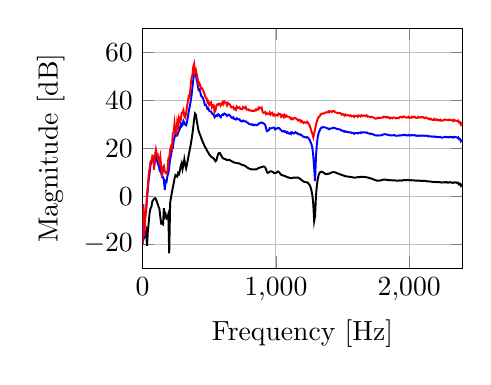
\begin{tikzpicture}

\begin{axis}[%
width=1.6in,
height=1.2in,
at={(1.011in,0.642in)},
scale only axis,
xmin=0,
xmax=2400,
xmajorgrids,
ymin=-30,
ymax=70,
ymajorgrids,
ylabel={Magnitude [dB]},
xlabel={Frequency [Hz]},
axis background/.style={fill=white}
]
\addplot [color=black,solid,line width=0.7pt,forget plot]
  table[row sep=crcr]{%
0	-20.0487587312399\\
6.66944096884746	-15.1198286488021\\
13.3388819376949	-17.0342399584206\\
20.0083229065424	-16.303194843339\\
26.6777638753898	-14.7962886511984\\
33.3472048442373	-20.6598371130847\\
40.0166458130848	-14.4557378448972\\
46.6860867819322	-10.7231796436896\\
53.3555277507797	-6.68929927164874\\
60.0249687196271	-5.00174395429775\\
66.6944096884746	-4.35120832215586\\
73.363850657322	-2.14327488039484\\
80.0332916261695	-1.6357351744986\\
86.702732595017	-1.08244168916939\\
93.3721735638644	-0.784791293115845\\
100.041614532712	-1.1515485217107\\
106.711055501559	-2.23392951885352\\
113.380496470407	-3.25334805655735\\
120.049937439254	-4.28723268538043\\
126.719378408102	-5.37856269568507\\
133.388819376949	-8.68574264179734\\
140.058260345797	-11.4500332968668\\
146.727701314644	-11.4038053561626\\
153.397142283492	-11.7245402057755\\
160.066583252339	-5.0055269896238\\
166.736024221186	-8.44545337311039\\
173.405465190034	-7.57504950140747\\
180.074906158881	-9.24310764770295\\
186.744347127729	-8.80698899348521\\
193.413788096576	-7.52181346110201\\
200.083229065424	-23.8498097372691\\
206.752670034271	-2.89005609350758\\
213.422111003119	-0.482574852395068\\
220.091551971966	1.60203735985558\\
226.760992940814	3.47424986688718\\
233.430433909661	5.29663217829555\\
240.099874878509	7.40902951539864\\
246.769315847356	8.79260541102708\\
253.438756816203	8.42229233177448\\
260.108197785051	8.1621822849779\\
266.777638753898	9.71860050383648\\
273.447079722746	9.24805783652312\\
280.116520691593	10.5461884815772\\
286.785961660441	12.7462393484334\\
293.455402629288	13.8128344559473\\
300.124843598136	11.3562980225335\\
306.794284566983	13.0225331345595\\
313.463725535831	15.3878277905346\\
320.133166504678	13.3487733331614\\
326.802607473525	11.618116409216\\
333.472048442373	13.2756561673794\\
340.14148941122	15.297365359007\\
346.810930380068	17.3666597314884\\
353.480371348915	19.1861707835379\\
360.149812317763	21.1548208550903\\
366.81925328661	23.2781736469893\\
373.488694255458	25.7795010023069\\
380.158135224305	28.7053918086881\\
386.827576193153	32.0846853382303\\
393.497017162	34.4267175381787\\
400.166458130848	33.9505458128728\\
406.835899099695	31.4873550826056\\
413.505340068542	29.2170117011374\\
420.17478103739	27.3019127159821\\
426.844222006237	26.1797366493716\\
433.513662975085	25.3157313050429\\
440.183103943932	24.2057182984711\\
446.85254491278	23.290395783258\\
453.521985881627	22.3878979183417\\
460.191426850475	21.60415932599\\
466.860867819322	20.7709829065924\\
473.53030878817	20.0885558968387\\
480.199749757017	19.4323228642096\\
486.869190725864	18.6908379824591\\
493.538631694712	18.1240856471387\\
500.208072663559	17.4169934799121\\
506.877513632407	16.986634280519\\
513.546954601254	16.4993581905569\\
520.216395570102	16.1919521224916\\
526.885836538949	16.0182134672153\\
533.555277507797	15.8037005327483\\
540.224718476644	15.1219659228159\\
546.894159445492	14.5825111378862\\
553.563600414339	14.9249330668376\\
560.233041383186	16.3345574651993\\
566.902482352034	17.5314472890824\\
573.571923320881	18.0466676213715\\
580.241364289729	17.9752767658784\\
586.910805258576	17.2620914846372\\
593.580246227424	16.6078538766868\\
600.249687196271	16.0282214291011\\
606.919128165119	15.6892443753367\\
613.588569133966	15.5882313206699\\
620.258010102814	15.4977489853147\\
626.927451071661	15.2498244875837\\
633.596892040508	15.0304027543537\\
640.266333009356	15.0950717833943\\
646.935773978203	15.2206054457582\\
653.605214947051	15.0570826579417\\
660.274655915898	14.8581503712255\\
666.944096884746	14.6159864112486\\
673.613537853593	14.4145622453499\\
680.282978822441	14.2407617757287\\
686.952419791288	14.0477359248121\\
693.621860760136	13.9845541892167\\
700.291301728983	13.9156960952036\\
706.960742697831	13.8209864026508\\
713.630183666678	13.7252040922125\\
720.299624635525	13.719919039345\\
726.969065604373	13.6610343852311\\
733.63850657322	13.4082141441493\\
740.307947542068	13.1756866771715\\
746.977388510915	13.0493516140333\\
753.646829479763	13.0081459317708\\
760.31627044861	12.8890321676709\\
766.985711417458	12.6553655249787\\
773.655152386305	12.5065721297099\\
780.324593355153	12.1476594869726\\
786.994034324	11.8745908760281\\
793.663475292847	11.7034903712762\\
800.332916261695	11.4985774792138\\
807.002357230542	11.3837332881055\\
813.67179819939	11.2277439431574\\
820.341239168237	11.2087216765361\\
827.010680137085	11.165959581749\\
833.680121105932	11.1324522724851\\
840.34956207478	11.2018621293156\\
847.019003043627	11.2058359789266\\
853.688444012475	11.220594143102\\
860.357884981322	11.385158335654\\
867.02732595017	11.6618138985397\\
873.696766919017	11.8074366257923\\
880.366207887864	11.9369555767766\\
887.035648856712	12.0897644436753\\
893.705089825559	12.1478349676403\\
900.374530794407	12.293869204835\\
907.043971763254	12.3962434453679\\
913.713412732102	12.2599054813914\\
920.382853700949	11.9560863463259\\
927.052294669797	11.0727027842254\\
933.721735638644	9.96470300024418\\
940.391176607492	9.75565988680186\\
947.060617576339	9.8817312233776\\
953.730058545186	10.2635241464301\\
960.399499514034	10.342564450562\\
967.068940482881	10.3395878261441\\
973.738381451729	10.1898658552898\\
980.407822420576	9.8934905161314\\
987.077263389424	9.66581752460281\\
993.746704358271	9.62786392512574\\
1000.41614532712	9.75615585236342\\
1007.08558629597	9.93971063557813\\
1013.75502726481	10.3422119903628\\
1020.42446823366	10.1980394823397\\
1027.09390920251	9.77924856044184\\
1033.76335017136	9.27605023907571\\
1040.4327911402	8.9026715525102\\
1047.10223210905	8.80362080534128\\
1053.7716730779	8.65318909923104\\
1060.44111404675	8.49430175012251\\
1067.11055501559	8.47806688429255\\
1073.77999598444	8.24819989854638\\
1080.44943695329	8.11312313460769\\
1087.11887792214	7.88692743852098\\
1093.78831889098	7.85693715538574\\
1100.45775985983	7.69465983381162\\
1107.12720082868	7.53269317692368\\
1113.79664179753	7.49971429912328\\
1120.46608276637	7.61271205995918\\
1127.13552373522	7.66843451521201\\
1133.80496470407	7.79602908681334\\
1140.47440567292	7.70448271239874\\
1147.14384664176	7.73221492909188\\
1153.81328761061	7.73181066779452\\
1160.48272857946	7.71857363461331\\
1167.15216954831	7.76954134955827\\
1173.82161051715	7.56221590613739\\
1180.491051486	7.23164524837447\\
1187.16049245485	7.0445338089638\\
1193.82993342369	6.68149349857916\\
1200.49937439254	6.4449899730087\\
1207.16881536139	6.10312875796965\\
1213.83825633024	6.0097646953722\\
1220.50769729908	5.87025384588163\\
1227.17713826793	5.8058226272411\\
1233.84657923678	5.78040134867712\\
1240.51602020563	5.59884417499817\\
1247.18546117447	5.02065144141591\\
1253.85490214332	4.61997118096475\\
1260.52434311217	3.67633292433192\\
1267.19378408102	2.34330760449349\\
1273.86322504986	0.330148903396033\\
1280.53266601871	-3.33406711562751\\
1287.20210698756	-10.2975077225615\\
1293.87154795641	-8.23932116173958\\
1300.54098892525	-0.0504526894621943\\
1307.2104298941	4.41312707327818\\
1313.87987086295	7.16388601945597\\
1320.5493118318	8.8180810705879\\
1327.21875280064	9.64769916783657\\
1333.88819376949	10.1213708572002\\
1340.55763473834	10.2126537699231\\
1347.22707570719	10.086236888369\\
1353.89651667603	9.96475533895285\\
1360.56595764488	9.68881796246233\\
1367.23539861373	9.45814374578669\\
1373.90483958258	9.21991209305461\\
1380.57428055142	9.22560189789232\\
1387.24372152027	9.25507050908739\\
1393.91316248912	9.39961014108227\\
1400.58260345797	9.40403399507104\\
1407.25204442681	9.5959632665098\\
1413.92148539566	9.81260026763373\\
1420.59092636451	9.9515380863488\\
1427.26036733336	10.0084243176538\\
1433.9298083022	10.076913415341\\
1440.59924927105	9.96583673695072\\
1447.2686902399	9.85390572621115\\
1453.93813120875	9.77057303062154\\
1460.60757217759	9.56658183325933\\
1467.27701314644	9.40119349335695\\
1473.94645411529	9.32365204414415\\
1480.61589508414	9.1400356094238\\
1487.28533605298	8.9782642045505\\
1493.95477702183	8.88490656734342\\
1500.62421799068	8.75658483707809\\
1507.29365895953	8.64394834471857\\
1513.96309992837	8.47813597782596\\
1520.63254089722	8.36366672323785\\
1527.30198186607	8.25947876297518\\
1533.97142283492	8.24130376763184\\
1540.64086380376	8.18123526644235\\
1547.31030477261	8.1022955122158\\
1553.97974574146	8.04006587529611\\
1560.64918671031	8.03334733158801\\
1567.31862767915	7.98098505634755\\
1573.988068648	7.88111469269561\\
1580.65750961685	7.8513820734062\\
1587.32695058569	7.73030446704829\\
1593.99639155454	7.74954898960166\\
1600.66583252339	7.81454036991847\\
1607.33527349224	7.83281535246582\\
1614.00471446108	7.94265737575515\\
1620.67415542993	7.98138741022576\\
1627.34359639878	7.98508389625216\\
1634.01303736763	8.04999617504294\\
1640.68247833647	8.10021289468602\\
1647.35191930532	8.06892639991748\\
1654.02136027417	8.05546864143061\\
1660.69080124302	8.06279491665488\\
1667.36024221186	7.97686673480105\\
1674.02968318071	7.95207358408032\\
1680.69912414956	7.90246757767181\\
1687.36856511841	7.77732599874859\\
1694.03800608725	7.74235995684231\\
1700.7074470561	7.57148021158726\\
1707.37688802495	7.51907183905363\\
1714.0463289938	7.34302575137448\\
1720.71576996264	7.29622254883677\\
1727.38521093149	7.10708183439396\\
1734.05465190034	6.99184506410273\\
1740.72409286919	6.81585864666285\\
1747.39353383803	6.73925074141611\\
1754.06297480688	6.51634814954277\\
1760.73241577573	6.5046366441454\\
1767.40185674458	6.51534274521224\\
1774.07129771342	6.49778597055656\\
1780.74073868227	6.5027309147596\\
1787.41017965112	6.66096272956585\\
1794.07962061997	6.68599174262566\\
1800.74906158881	6.7859138904786\\
1807.41850255766	6.93749707775066\\
1814.08794352651	6.93925297520513\\
1820.75738449536	6.92244091960105\\
1827.4268254642	6.88417990649145\\
1834.09626643305	6.72060751795472\\
1840.7657074019	6.68313612027974\\
1847.43514837075	6.76439558492782\\
1854.10458933959	6.62118179284594\\
1860.77403030844	6.67666591156341\\
1867.44347127729	6.66742931604751\\
1874.11291224614	6.61812127334921\\
1880.78235321498	6.57379594203512\\
1887.45179418383	6.6252911037417\\
1894.12123515268	6.58083432296879\\
1900.79067612153	6.52814176468354\\
1907.46011709037	6.50124438101973\\
1914.12955805922	6.53921917902875\\
1920.79899902807	6.50564465486567\\
1927.46843999692	6.59670977440938\\
1934.13788096576	6.5808210246406\\
1940.80732193461	6.5207010147943\\
1947.47676290346	6.51506968513275\\
1954.14620387231	6.73310819944533\\
1960.81564484115	6.71013860894114\\
1967.48508581	6.64903913507737\\
1974.15452677885	6.74812319759256\\
1980.82396774769	6.71068768316015\\
1987.49340871654	6.66610261621373\\
1994.16284968539	6.76891694050447\\
2000.83229065424	6.6491896391241\\
2007.50173162308	6.61585957804051\\
2014.17117259193	6.69663297716651\\
2020.84061356078	6.63556782623735\\
2027.51005452963	6.61496288121215\\
2034.17949549847	6.65314733859702\\
2040.84893646732	6.56253815480099\\
2047.51837743617	6.52719414236225\\
2054.18781840502	6.53288683163146\\
2060.85725937386	6.44397445046302\\
2067.52670034271	6.52132437447671\\
2074.19614131156	6.45651887990799\\
2080.86558228041	6.49180231444652\\
2087.53502324925	6.37556254246593\\
2094.2044642181	6.38835955815856\\
2100.87390518695	6.38800999197321\\
2107.5433461558	6.41869017506372\\
2114.21278712464	6.45696129007083\\
2120.88222809349	6.38399284967227\\
2127.55166906234	6.30427827094713\\
2134.22111003119	6.19580379642489\\
2140.89055100003	6.23445392444571\\
2147.55999196888	6.138755636176\\
2154.22943293773	6.15874396802726\\
2160.89887390658	6.08763548342839\\
2167.56831487542	6.03555632613822\\
2174.23775584427	5.98609086606414\\
2180.90719681312	6.02482885091038\\
2187.57663778197	5.91142930127247\\
2194.24607875081	5.90620837397779\\
2200.91551971966	5.97642482649767\\
2207.58496068851	5.8267910718678\\
2214.25440165736	5.89031841840725\\
2220.9238426262	5.89135869621277\\
2227.59328359505	5.89733460682358\\
2234.2627245639	5.80541657746534\\
2240.93216553275	5.68604121080201\\
2247.60160650159	5.75738242073362\\
2254.27104747044	5.79181508953615\\
2260.94048843929	5.72435541249592\\
2267.60992940814	5.91887483795505\\
2274.27937037698	5.74323479651245\\
2280.94881134583	5.915516734774\\
2287.61825231468	5.678546930139\\
2294.28769328353	5.66300396208394\\
2300.95713425237	5.8598982127844\\
2307.62657522122	5.83660940155178\\
2314.29601619007	5.65455921049519\\
2320.96545715892	5.72882209801376\\
2327.63489812776	5.55231206649722\\
2334.30433909661	5.77650458704093\\
2340.97378006546	5.67908113685681\\
2347.64322103431	5.80773692997328\\
2354.31266200315	5.69838419206977\\
2360.982102972	5.40321555955911\\
2367.65154394085	5.64298798739372\\
2374.3209849097	4.92864224564267\\
2380.99042587854	5.18402670886947\\
2387.65986684739	4.4041843097699\\
2394.32930781624	5.21405865383168\\
};
\addplot [color=blue,line width=0.7pt,solid,forget plot]
  table[row sep=crcr]{%
0	-19.1801970800519\\
6.66944096884746	-12.8703566346097\\
13.3388819376949	-14.9767747928368\\
20.0083229065424	-8.1169528748585\\
26.6777638753898	-6.02007700819861\\
33.3472048442373	-0.983876052705199\\
40.0166458130848	3.03834920475862\\
46.6860867819322	7.17636581805885\\
53.3555277507797	9.86526177201357\\
60.0249687196271	13.1463387708932\\
66.6944096884746	13.8757372547918\\
73.363850657322	15.3344350669251\\
80.0332916261695	15.5103872374769\\
86.702732595017	16.425478329494\\
93.3721735638644	14.7417155654727\\
100.041614532712	16.8909416893169\\
106.711055501559	15.1693140361402\\
113.380496470407	13.8378835887887\\
120.049937439254	12.8763175666628\\
126.719378408102	11.2245842269512\\
133.388819376949	12.2755448015368\\
140.058260345797	9.76444174431159\\
146.727701314644	7.9812499771494\\
153.397142283492	7.89449997979367\\
160.066583252339	6.76913976316376\\
166.736024221186	2.64501448882146\\
173.405465190034	6.32166739159555\\
180.074906158881	6.03588448839818\\
186.744347127729	8.53733258644788\\
193.413788096576	9.60386927649499\\
200.083229065424	11.9079525145153\\
206.752670034271	15.5768450064805\\
213.422111003119	16.8564773229072\\
220.091551971966	19.4056208174385\\
226.760992940814	20.0977881758406\\
233.430433909661	23.0867696537098\\
240.099874878509	24.5133525415327\\
246.769315847356	26.0318705836573\\
253.438756816203	25.2159191534437\\
260.108197785051	25.3004400529391\\
266.777638753898	26.3567739565968\\
273.447079722746	27.4030394355481\\
280.116520691593	28.0266175894058\\
286.785961660441	30.3237158950793\\
293.455402629288	29.2015400170774\\
300.124843598136	29.6615334869133\\
306.794284566983	31.3788778937628\\
313.463725535831	30.6152438924125\\
320.133166504678	29.7759228465178\\
326.802607473525	29.5619250778803\\
333.472048442373	31.0231998781484\\
340.14148941122	32.9915165065272\\
346.810930380068	35.5603667608652\\
353.480371348915	37.1554836973345\\
360.149812317763	39.2773434425713\\
366.81925328661	41.5981250326168\\
373.488694255458	44.9696288263719\\
380.158135224305	48.3111948726315\\
386.827576193153	51.2585070598154\\
393.497017162	51.2682639867973\\
400.166458130848	50.243525737973\\
406.835899099695	48.4862480361356\\
413.505340068542	46.2836446546836\\
420.17478103739	44.3104281370761\\
426.844222006237	44.5172237794285\\
433.513662975085	43.2209471111121\\
440.183103943932	41.6709460714875\\
446.85254491278	41.4697262151817\\
453.521985881627	40.7647867182055\\
460.191426850475	39.6633007472136\\
466.860867819322	38.0957284486303\\
473.53030878817	38.169121432027\\
480.199749757017	37.4519012732778\\
486.869190725864	36.3727934222095\\
493.538631694712	36.5546229678987\\
500.208072663559	35.5969432067736\\
506.877513632407	35.367941821441\\
513.546954601254	35.2417809028389\\
520.216395570102	34.6477493524093\\
526.885836538949	34.1244046315677\\
533.555277507797	34.1031174062651\\
540.224718476644	32.9038375330107\\
546.894159445492	33.3928388176014\\
553.563600414339	33.7323160866798\\
560.233041383186	33.4368130917103\\
566.902482352034	34.1904953640828\\
573.571923320881	33.931489848504\\
580.241364289729	33.3392737176728\\
586.910805258576	32.8984144124481\\
593.580246227424	33.7433695622489\\
600.249687196271	34.1178753654268\\
606.919128165119	33.9336683252705\\
613.588569133966	34.4485544577773\\
620.258010102814	34.2843657671703\\
626.927451071661	34.060214309503\\
633.596892040508	33.4349764550008\\
640.266333009356	33.8646627251901\\
646.935773978203	33.9786137674422\\
653.605214947051	33.7465785637577\\
660.274655915898	33.3109087036117\\
666.944096884746	32.7438776079588\\
673.613537853593	32.568638059062\\
680.282978822441	32.9108736275211\\
686.952419791288	32.2249942772816\\
693.621860760136	32.1142750583997\\
700.291301728983	31.9571324211216\\
706.960742697831	32.4892728441236\\
713.630183666678	32.1435994092285\\
720.299624635525	32.021746854411\\
726.969065604373	32.0710323808955\\
733.63850657322	31.4267831219643\\
740.307947542068	31.1772695382483\\
746.977388510915	31.162518285872\\
753.646829479763	31.5393637388437\\
760.31627044861	31.2973953950049\\
766.985711417458	31.2182846338879\\
773.655152386305	31.2160961127834\\
780.324593355153	30.8348945075471\\
786.994034324	30.7286324748179\\
793.663475292847	30.382857168758\\
800.332916261695	30.0744778419275\\
807.002357230542	29.9962664433648\\
813.67179819939	29.962698019713\\
820.341239168237	29.6686337884023\\
827.010680137085	29.9415857655778\\
833.680121105932	29.665781211827\\
840.34956207478	29.6266816144405\\
847.019003043627	29.8283984647226\\
853.688444012475	29.6297069262368\\
860.357884981322	29.6061515105809\\
867.02732595017	29.9255274703579\\
873.696766919017	30.3836449587776\\
880.366207887864	30.4195349481781\\
887.035648856712	30.6293093173666\\
893.705089825559	30.7583945440376\\
900.374530794407	30.4889757351797\\
907.043971763254	30.3845402431785\\
913.713412732102	30.04889124241\\
920.382853700949	29.6944489814507\\
927.052294669797	28.0784153048193\\
933.721735638644	27.1086812359051\\
940.391176607492	27.3559333536648\\
947.060617576339	27.5405458598276\\
953.730058545186	28.3388139097659\\
960.399499514034	28.2741413233711\\
967.068940482881	28.316457653925\\
973.738381451729	28.5072210913902\\
980.407822420576	28.5600053986234\\
987.077263389424	28.5737552132371\\
993.746704358271	27.8398963271317\\
1000.41614532712	28.0898809053163\\
1007.08558629597	28.1965674308498\\
1013.75502726481	28.4628748764566\\
1020.42446823366	28.4109689957096\\
1027.09390920251	28.3068645746434\\
1033.76335017136	27.7346741698898\\
1040.4327911402	27.4788041500008\\
1047.10223210905	27.0100829685413\\
1053.7716730779	26.9924831726905\\
1060.44111404675	27.2004924387251\\
1067.11055501559	26.849233187843\\
1073.77999598444	26.9830257865469\\
1080.44943695329	26.4670906903599\\
1087.11887792214	26.7454074919348\\
1093.78831889098	26.1231981345171\\
1100.45775985983	26.0690493476289\\
1107.12720082868	26.4257190724241\\
1113.79664179753	25.9698837825955\\
1120.46608276637	26.6504318008235\\
1127.13552373522	26.3755217205762\\
1133.80496470407	26.1354915787008\\
1140.47440567292	26.4380891246027\\
1147.14384664176	26.6813208161658\\
1153.81328761061	26.2404976832252\\
1160.48272857946	26.322558600175\\
1167.15216954831	25.8835037848182\\
1173.82161051715	25.7364256243679\\
1180.491051486	25.8250596096695\\
1187.16049245485	25.4196005650628\\
1193.82993342369	25.4691538328777\\
1200.49937439254	25.0421318570829\\
1207.16881536139	24.7441917848824\\
1213.83825633024	24.5748943582446\\
1220.50769729908	24.5925564266071\\
1227.17713826793	24.4302692146368\\
1233.84657923678	24.6810745589517\\
1240.51602020563	24.397307782136\\
1247.18546117447	23.908083233262\\
1253.85490214332	23.4238712415594\\
1260.52434311217	22.5052907976336\\
1267.19378408102	21.5606708818796\\
1273.86322504986	20.0584900520215\\
1280.53266601871	16.6940016155194\\
1287.20210698756	11.6522752349905\\
1293.87154795641	6.30451494354049\\
1300.54098892525	16.4372208246285\\
1307.2104298941	21.5531699253565\\
1313.87987086295	24.6671956263859\\
1320.5493118318	26.3379178804065\\
1327.21875280064	27.1813964983545\\
1333.88819376949	28.0484733159775\\
1340.55763473834	28.6069160984365\\
1347.22707570719	28.5982246304511\\
1353.89651667603	28.8769385917799\\
1360.56595764488	28.7223173527069\\
1367.23539861373	28.6659731656965\\
1373.90483958258	28.5922594637542\\
1380.57428055142	28.4587951765109\\
1387.24372152027	28.2085080700907\\
1393.91316248912	28.2150230654651\\
1400.58260345797	27.8900350269182\\
1407.25204442681	28.1925719408122\\
1413.92148539566	28.2419799953219\\
1420.59092636451	28.2829268523402\\
1427.26036733336	28.4634872164612\\
1433.9298083022	28.5907769115149\\
1440.59924927105	28.3814763609529\\
1447.2686902399	28.3226799307106\\
1453.93813120875	28.1356741426561\\
1460.60757217759	27.9685526227807\\
1467.27701314644	27.9678715914959\\
1473.94645411529	27.8909541343816\\
1480.61589508414	27.8238766711262\\
1487.28533605298	27.6014302681019\\
1493.95477702183	27.2717380592555\\
1500.62421799068	27.3018413746368\\
1507.29365895953	27.1995224671422\\
1513.96309992837	26.8397200608697\\
1520.63254089722	27.0829515584527\\
1527.30198186607	26.8503571067805\\
1533.97142283492	26.756386803348\\
1540.64086380376	26.7898604834281\\
1547.31030477261	26.6321969857586\\
1553.97974574146	26.6120446351326\\
1560.64918671031	26.6522550973329\\
1567.31862767915	26.3323931160699\\
1573.988068648	26.4295250363119\\
1580.65750961685	26.343839184407\\
1587.32695058569	26.0015876489182\\
1593.99639155454	26.3300221476214\\
1600.66583252339	26.3039705741923\\
1607.33527349224	26.3742650558845\\
1614.00471446108	26.1463871584589\\
1620.67415542993	26.4418942251999\\
1627.34359639878	26.4672180007292\\
1634.01303736763	26.2792446290963\\
1640.68247833647	26.6436284243602\\
1647.35191930532	26.5095040190372\\
1654.02136027417	26.6573687967465\\
1660.69080124302	26.5620677867498\\
1667.36024221186	26.5989978419798\\
1674.02968318071	26.4764653674816\\
1680.69912414956	26.6013987294364\\
1687.36856511841	26.2507565066588\\
1694.03800608725	26.250822684696\\
1700.7074470561	26.1437788317374\\
1707.37688802495	26.0138276096747\\
1714.0463289938	26.0000044652493\\
1720.71576996264	25.9766429547442\\
1727.38521093149	25.7852372119412\\
1734.05465190034	25.6845896433477\\
1740.72409286919	25.4260848492213\\
1747.39353383803	25.3815678004591\\
1754.06297480688	25.3994084234738\\
1760.73241577573	25.2465614318773\\
1767.40185674458	25.3585533383756\\
1774.07129771342	25.2934182835509\\
1780.74073868227	25.3332686921627\\
1787.41017965112	25.3315671007097\\
1794.07962061997	25.4529797134563\\
1800.74906158881	25.5886581256154\\
1807.41850255766	25.8112219394707\\
1814.08794352651	25.8336747007692\\
1820.75738449536	25.8512388544852\\
1827.4268254642	25.6812476695809\\
1834.09626643305	25.7200303426687\\
1840.7657074019	25.5997689689591\\
1847.43514837075	25.6166191632788\\
1854.10458933959	25.361021151081\\
1860.77403030844	25.4169823389784\\
1867.44347127729	25.3575452873573\\
1874.11291224614	25.3531107579859\\
1880.78235321498	25.4061044547324\\
1887.45179418383	25.4934789583337\\
1894.12123515268	25.2934729566871\\
1900.79067612153	25.150524012892\\
1907.46011709037	25.2282774494811\\
1914.12955805922	25.2017626260044\\
1920.79899902807	25.2044661735462\\
1927.46843999692	25.3815455806729\\
1934.13788096576	25.3764459878828\\
1940.80732193461	25.385750006199\\
1947.47676290346	25.3633905907365\\
1954.14620387231	25.5519570739233\\
1960.81564484115	25.6353093777738\\
1967.48508581	25.4451022627762\\
1974.15452677885	25.4541836251086\\
1980.82396774769	25.337687037348\\
1987.49340871654	25.3510653476931\\
1994.16284968539	25.5605415694349\\
2000.83229065424	25.2743306829669\\
2007.50173162308	25.3800826099287\\
2014.17117259193	25.3329161570438\\
2020.84061356078	25.5531143426426\\
2027.51005452963	25.3941264714679\\
2034.17949549847	25.347106390821\\
2040.84893646732	25.4895692062649\\
2047.51837743617	25.2661215623274\\
2054.18781840502	25.2210476794\\
2060.85725937386	25.1367687606202\\
2067.52670034271	25.3569013486922\\
2074.19614131156	25.1900684754222\\
2080.86558228041	25.1789893140517\\
2087.53502324925	25.2859951981971\\
2094.2044642181	25.172839426885\\
2100.87390518695	25.2515733216014\\
2107.5433461558	25.2880714341211\\
2114.21278712464	25.1545719013543\\
2120.88222809349	25.2268960929446\\
2127.55166906234	25.2355614416271\\
2134.22111003119	25.0702603234227\\
2140.89055100003	25.1476689770138\\
2147.55999196888	24.9247159902261\\
2154.22943293773	24.922689731992\\
2160.89887390658	24.9955133770923\\
2167.56831487542	24.8149518125789\\
2174.23775584427	24.8259792113246\\
2180.90719681312	24.7869406198621\\
2187.57663778197	24.9333284802604\\
2194.24607875081	24.7182320239595\\
2200.91551971966	24.7419174388744\\
2207.58496068851	24.7876142318302\\
2214.25440165736	24.6259659842357\\
2220.9238426262	24.6350924557445\\
2227.59328359505	24.598620967243\\
2234.2627245639	24.7247842187087\\
2240.93216553275	24.4098973625254\\
2247.60160650159	24.4556792725291\\
2254.27104747044	24.5283713595465\\
2260.94048843929	24.5861744693618\\
2267.60992940814	24.7581537657624\\
2274.27937037698	24.6396803738645\\
2280.94881134583	24.654846607342\\
2287.61825231468	24.5997381831205\\
2294.28769328353	24.5289027956748\\
2300.95713425237	24.7571708595127\\
2307.62657522122	24.5896255439116\\
2314.29601619007	24.6110451864451\\
2320.96545715892	24.667921486107\\
2327.63489812776	24.3877408742219\\
2334.30433909661	24.7693625782859\\
2340.97378006546	24.6509753376336\\
2347.64322103431	24.6243542594069\\
2354.31266200315	24.545777701483\\
2360.982102972	24.3907721668534\\
2367.65154394085	24.5803582147782\\
2374.3209849097	23.7571480890376\\
2380.99042587854	23.8421940134045\\
2387.65986684739	22.9126274129111\\
2394.32930781624	23.5765876365837\\
};
\addplot [color=red,line width=0.7pt,solid,forget plot]
  table[row sep=crcr]{%
0	-19.7731498838748\\
6.66944096884746	-3.30129229121397\\
13.3388819376949	-16.5196915187148\\
20.0083229065424	-9.14668053363022\\
26.6777638753898	-5.76166775232025\\
33.3472048442373	0.715997976350927\\
40.0166458130848	4.67569859122506\\
46.6860867819322	9.3061016685291\\
53.3555277507797	11.6803761046995\\
60.0249687196271	14.5668135581482\\
66.6944096884746	14.7654268062205\\
73.363850657322	16.719238826743\\
80.0332916261695	16.1424633419342\\
86.702732595017	11.0575281883368\\
93.3721735638644	17.1794418502135\\
100.041614532712	19.4302729226033\\
106.711055501559	17.1647243810114\\
113.380496470407	17.4336984563287\\
120.049937439254	14.8178077949204\\
126.719378408102	14.0940850084646\\
133.388819376949	16.3749922926234\\
140.058260345797	12.5351765733749\\
146.727701314644	8.12594321424465\\
153.397142283492	11.8920519865686\\
160.066583252339	12.5716166006834\\
166.736024221186	10.285037659743\\
173.405465190034	9.70252691083641\\
180.074906158881	9.57652623134213\\
186.744347127729	10.638286473325\\
193.413788096576	15.8057440036925\\
200.083229065424	16.2967711522382\\
206.752670034271	19.4251561642881\\
213.422111003119	20.6816823950601\\
220.091551971966	19.8519442653404\\
226.760992940814	26.1082556453237\\
233.430433909661	26.6500868664063\\
240.099874878509	30.404475221027\\
246.769315847356	26.825393131967\\
253.438756816203	26.1285404111887\\
260.108197785051	30.9570292670671\\
266.777638753898	29.2117125593558\\
273.447079722746	32.6064626863794\\
280.116520691593	31.2360770691429\\
286.785961660441	31.722505229895\\
293.455402629288	34.6999692669045\\
300.124843598136	34.9927928087575\\
306.794284566983	35.8925128734339\\
313.463725535831	33.3145155986805\\
320.133166504678	32.8004219522627\\
326.802607473525	34.6908681946822\\
333.472048442373	37.2792444982084\\
340.14148941122	39.6336780746653\\
346.810930380068	41.6658226560305\\
353.480371348915	41.2799335430523\\
360.149812317763	45.6293609227908\\
366.81925328661	49.1313794764531\\
373.488694255458	50.4146591961717\\
380.158135224305	53.8841719664011\\
386.827576193153	55.1607782592531\\
393.497017162	51.6507310675641\\
400.166458130848	52.5696601172965\\
406.835899099695	50.685373547418\\
413.505340068542	48.8997703515724\\
420.17478103739	46.055352278522\\
426.844222006237	46.9843441763525\\
433.513662975085	46.0167755931766\\
440.183103943932	44.7586647963142\\
446.85254491278	44.899210692511\\
453.521985881627	44.2825029563711\\
460.191426850475	43.3405779426588\\
466.860867819322	42.2331601158757\\
473.53030878817	40.9054822858416\\
480.199749757017	40.8005939018429\\
486.869190725864	39.1794932936421\\
493.538631694712	39.5687046720476\\
500.208072663559	38.0284570137054\\
506.877513632407	38.6610399513643\\
513.546954601254	39.0673385461637\\
520.216395570102	37.1510698815421\\
526.885836538949	37.9929142604868\\
533.555277507797	37.8986469335816\\
540.224718476644	35.0617599237344\\
546.894159445492	35.684870669366\\
553.563600414339	37.7578937591971\\
560.233041383186	38.24050111937\\
566.902482352034	38.016164070372\\
573.571923320881	38.6115137612817\\
580.241364289729	38.5083844553459\\
586.910805258576	37.7271324115351\\
593.580246227424	38.4959940201515\\
600.249687196271	39.142060156938\\
606.919128165119	38.3708394010276\\
613.588569133966	39.4929000003076\\
620.258010102814	39.0343745804699\\
626.927451071661	39.0045192335195\\
633.596892040508	37.87804477622\\
640.266333009356	38.8658497847705\\
646.935773978203	38.5200866414581\\
653.605214947051	38.2617127986245\\
660.274655915898	37.6673340406495\\
666.944096884746	36.942659357658\\
673.613537853593	37.0599783142805\\
680.282978822441	37.2310736462357\\
686.952419791288	36.2838048671267\\
693.621860760136	36.550554058913\\
700.291301728983	35.9917952535513\\
706.960742697831	37.3200057510477\\
713.630183666678	36.793136905267\\
720.299624635525	36.8249417546396\\
726.969065604373	37.0781762663894\\
733.63850657322	36.4125402477533\\
740.307947542068	36.3121785296935\\
746.977388510915	36.2451162273039\\
753.646829479763	37.2084380506257\\
760.31627044861	36.9206850342757\\
766.985711417458	36.6914275508524\\
773.655152386305	37.2095095164535\\
780.324593355153	36.104968563149\\
786.994034324	36.048838049227\\
793.663475292847	36.190495756928\\
800.332916261695	35.7104287884522\\
807.002357230542	35.8242109649086\\
813.67179819939	35.6991761345302\\
820.341239168237	35.4503876709311\\
827.010680137085	35.6718081181175\\
833.680121105932	35.5252868419793\\
840.34956207478	35.5637592153987\\
847.019003043627	36.1216316480192\\
853.688444012475	35.8541719470195\\
860.357884981322	36.3190619987209\\
867.02732595017	36.1211510307247\\
873.696766919017	37.056863223976\\
880.366207887864	36.651127915307\\
887.035648856712	36.5825166509355\\
893.705089825559	36.9504055566917\\
900.374530794407	35.1961814758886\\
907.043971763254	34.7039472643645\\
913.713412732102	34.8894998271584\\
920.382853700949	35.1129229272755\\
927.052294669797	34.2035062965127\\
933.721735638644	34.544536166122\\
940.391176607492	34.3161625921429\\
947.060617576339	34.2152352021431\\
953.730058545186	34.9725599786183\\
960.399499514034	34.0157821012478\\
967.068940482881	34.5575512902624\\
973.738381451729	34.7924069441786\\
980.407822420576	33.7202383105071\\
987.077263389424	34.0640499711664\\
993.746704358271	33.5499848673986\\
1000.41614532712	33.7602055880614\\
1007.08558629597	33.8794047458212\\
1013.75502726481	33.6000643803354\\
1020.42446823366	34.41709105744\\
1027.09390920251	34.1784844968047\\
1033.76335017136	34.213559194249\\
1040.4327911402	33.0793653419113\\
1047.10223210905	33.5387825724225\\
1053.7716730779	33.824912673582\\
1060.44111404675	32.9699657541057\\
1067.11055501559	33.8378469138417\\
1073.77999598444	33.2124005244341\\
1080.44943695329	33.5671937553562\\
1087.11887792214	33.1124632723943\\
1093.78831889098	33.1180967971584\\
1100.45775985983	33.1098632608928\\
1107.12720082868	32.6414362236894\\
1113.79664179753	32.1194058224594\\
1120.46608276637	32.5272282197209\\
1127.13552373522	32.0840721791977\\
1133.80496470407	32.4943251641124\\
1140.47440567292	32.5364569322681\\
1147.14384664176	32.5852481246147\\
1153.81328761061	32.1751862503957\\
1160.48272857946	31.9964871334953\\
1167.15216954831	31.5145565174944\\
1173.82161051715	31.9319084355698\\
1180.491051486	31.6954106176743\\
1187.16049245485	31.0173995293861\\
1193.82993342369	31.4179436596554\\
1200.49937439254	30.88197629505\\
1207.16881536139	30.4987820836591\\
1213.83825633024	30.8907166745812\\
1220.50769729908	30.669066786967\\
1227.17713826793	30.6088276123375\\
1233.84657923678	31.0230605872693\\
1240.51602020563	30.646974834486\\
1247.18546117447	30.0056944791357\\
1253.85490214332	29.3534461723242\\
1260.52434311217	28.2651209471615\\
1267.19378408102	26.954021048548\\
1273.86322504986	25.9012974545492\\
1280.53266601871	24.5716215147262\\
1287.20210698756	26.1838866071504\\
1293.87154795641	27.9640423038921\\
1300.54098892525	29.6587510669448\\
1307.2104298941	31.1844476112175\\
1313.87987086295	32.2512424614966\\
1320.5493118318	33.0744916232722\\
1327.21875280064	33.1938211374655\\
1333.88819376949	33.8594312519506\\
1340.55763473834	34.3239227849652\\
1347.22707570719	34.2903123904882\\
1353.89651667603	34.5362555107921\\
1360.56595764488	34.4735651034455\\
1367.23539861373	34.6424254058558\\
1373.90483958258	34.9998993126672\\
1380.57428055142	34.9445366157403\\
1387.24372152027	34.9212782294764\\
1393.91316248912	35.3210359275985\\
1400.58260345797	34.957042662985\\
1407.25204442681	35.4463006533749\\
1413.92148539566	35.3815415899574\\
1420.59092636451	35.1247290520045\\
1427.26036733336	35.483454745991\\
1433.9298083022	35.5680035110321\\
1440.59924927105	35.2443526361233\\
1447.2686902399	34.9585356085181\\
1453.93813120875	34.8467609647867\\
1460.60757217759	34.6729699561945\\
1467.27701314644	34.5901111077368\\
1473.94645411529	34.7679439086908\\
1480.61589508414	34.6966283625407\\
1487.28533605298	34.4917011620637\\
1493.95477702183	33.9895974859901\\
1500.62421799068	34.219971740426\\
1507.29365895953	34.0773365592971\\
1513.96309992837	33.5919233073209\\
1520.63254089722	34.05674398874\\
1527.30198186607	33.6836839894487\\
1533.97142283492	33.737728138333\\
1540.64086380376	33.8784614848418\\
1547.31030477261	33.6511509515165\\
1553.97974574146	33.4226620143495\\
1560.64918671031	33.6968369088947\\
1567.31862767915	33.276016797193\\
1573.988068648	33.5366942634168\\
1580.65750961685	33.5209888551424\\
1587.32695058569	33.0236853121862\\
1593.99639155454	33.5420262045134\\
1600.66583252339	33.492102025589\\
1607.33527349224	33.5873714387896\\
1614.00471446108	33.0923914795437\\
1620.67415542993	33.6676565539402\\
1627.34359639878	33.564976523811\\
1634.01303736763	33.260843386433\\
1640.68247833647	33.6986835385745\\
1647.35191930532	33.4190163219924\\
1654.02136027417	33.6411712118615\\
1660.69080124302	33.5615313638007\\
1667.36024221186	33.564357460058\\
1674.02968318071	33.3931136236589\\
1680.69912414956	33.7027218290536\\
1687.36856511841	33.153902660869\\
1694.03800608725	33.2556036519438\\
1700.7074470561	33.1633921770775\\
1707.37688802495	32.971772759543\\
1714.0463289938	33.0718132268812\\
1720.71576996264	33.0923277218807\\
1727.38521093149	32.8549585330854\\
1734.05465190034	32.7263913958038\\
1740.72409286919	32.4113821233463\\
1747.39353383803	32.3581318999144\\
1754.06297480688	32.5013000771757\\
1760.73241577573	32.397506990593\\
1767.40185674458	32.762027196197\\
1774.07129771342	32.6426044719977\\
1780.74073868227	32.5927768254359\\
1787.41017965112	32.6550171941744\\
1794.07962061997	32.7793490227485\\
1800.74906158881	32.7079221015991\\
1807.41850255766	33.1481905312322\\
1814.08794352651	33.0278793087225\\
1820.75738449536	33.1230239360321\\
1827.4268254642	32.8213517278662\\
1834.09626643305	33.0357032185694\\
1840.7657074019	32.7839350712744\\
1847.43514837075	32.9292949378254\\
1854.10458933959	32.4314197720893\\
1860.77403030844	32.7096293453212\\
1867.44347127729	32.6528396080951\\
1874.11291224614	32.446351701142\\
1880.78235321498	32.7719434715459\\
1887.45179418383	32.8660899906374\\
1894.12123515268	32.7054232709123\\
1900.79067612153	32.4172726216336\\
1907.46011709037	32.5655138262646\\
1914.12955805922	32.6899357772568\\
1920.79899902807	32.4907240301219\\
1927.46843999692	32.9278271785415\\
1934.13788096576	33.0360239620291\\
1940.80732193461	33.0176444262547\\
1947.47676290346	32.7593496869112\\
1954.14620387231	33.1663282462649\\
1960.81564484115	33.2507591912716\\
1967.48508581	32.972874509728\\
1974.15452677885	32.8277872601022\\
1980.82396774769	32.7746222144784\\
1987.49340871654	32.734742518744\\
1994.16284968539	33.1215205897337\\
2000.83229065424	32.6914518434221\\
2007.50173162308	32.7559968712182\\
2014.17117259193	32.677494916305\\
2020.84061356078	33.1664443003249\\
2027.51005452963	32.8962902999062\\
2034.17949549847	32.8384791907013\\
2040.84893646732	33.1302460915559\\
2047.51837743617	32.7275270964612\\
2054.18781840502	32.7021585046661\\
2060.85725937386	32.6287144507275\\
2067.52670034271	33.0835777879169\\
2074.19614131156	32.794345139603\\
2080.86558228041	32.7793950077453\\
2087.53502324925	32.9691533338572\\
2094.2044642181	32.8349283445452\\
2100.87390518695	33.0040625609765\\
2107.5433461558	32.9034999051104\\
2114.21278712464	32.5325190511779\\
2120.88222809349	32.7901048188627\\
2127.55166906234	32.7906003194698\\
2134.22111003119	32.4246517958174\\
2140.89055100003	32.4716819019555\\
2147.55999196888	32.0984015814186\\
2154.22943293773	32.0613549788269\\
2160.89887390658	32.3383445893988\\
2167.56831487542	31.8703975029692\\
2174.23775584427	31.8429764048798\\
2180.90719681312	31.8019842458616\\
2187.57663778197	32.2476589009584\\
2194.24607875081	31.8144992473476\\
2200.91551971966	31.8431698502412\\
2207.58496068851	32.0456705923427\\
2214.25440165736	31.593171855717\\
2220.9238426262	31.6858001737609\\
2227.59328359505	31.6328584571135\\
2234.2627245639	31.8788570701691\\
2240.93216553275	31.4446130819145\\
2247.60160650159	31.5207907638188\\
2254.27104747044	31.6020271775451\\
2260.94048843929	31.8038303030393\\
2267.60992940814	31.9799425725219\\
2274.27937037698	31.8728007578464\\
2280.94881134583	31.7598315159353\\
2287.61825231468	31.7560594104097\\
2294.28769328353	31.6520730552651\\
2300.95713425237	31.9183257282884\\
2307.62657522122	31.654108360502\\
2314.29601619007	31.6740489966585\\
2320.96545715892	31.7499951489144\\
2327.63489812776	31.3009481697144\\
2334.30433909661	31.7980891319717\\
2340.97378006546	31.493448553402\\
2347.64322103431	31.5929740708855\\
2354.31266200315	31.3397381174602\\
2360.982102972	31.3624305660842\\
2367.65154394085	31.5463110546057\\
2374.3209849097	30.6428752516702\\
2380.99042587854	30.8147671870351\\
2387.65986684739	29.9134672047925\\
2394.32930781624	30.7874812765343\\
};
\end{axis}
\end{tikzpicture}%
	\caption{Driver tests.}
	\label{fig:freq_responsedrivercomb}
\end{subfigure}
\begin{subfigure}[t]{0.28\textwidth}
	\tikzsetnextfilename{FFT_enclosure_comb}
	% This file was created by matlab2tikz.
%
%The latest updates can be retrieved from
%  http://www.mathworks.com/matlabcentral/fileexchange/22022-matlab2tikz-matlab2tikz
%where you can also make suggestions and rate matlab2tikz.
%
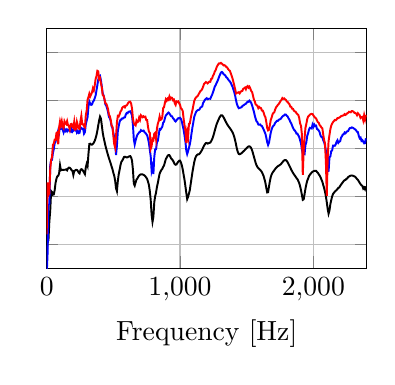
\begin{tikzpicture}

\begin{axis}[%
width=1.6in,
height=1.2in,
at={(1.011in,0.642in)},
scale only axis,
xmin=0,
xmax=2400,
xmajorgrids,
ymin=-30,
ymax=70,
ymajorgrids,
yticklabels={\empty},
xlabel={Frequency [Hz]},
axis background/.style={fill=white}
]
\addplot [color=black,solid,line width=0.7pt,forget plot]
  table[row sep=crcr]{%
0	-24.0683456294169\\
6.66944096884746	-19.3396560250162\\
13.3388819376949	-18.2831164389234\\
20.0083229065424	-10.6084546004752\\
26.6777638753898	-5.97086599305024\\
33.3472048442373	2.16522108527114\\
40.0166458130848	1.75978395548184\\
46.6860867819322	0.626734426887425\\
53.3555277507797	0.737871732712977\\
60.0249687196271	2.52580920909833\\
66.6944096884746	5.58384561111023\\
73.363850657322	7.31560850076007\\
80.0332916261695	8.28717488787875\\
86.702732595017	8.53458853640431\\
93.3721735638644	9.53756253011135\\
100.041614532712	12.9013120736345\\
106.711055501559	10.7979139982812\\
113.380496470407	11.0003823416785\\
120.049937439254	10.9780806423727\\
126.719378408102	10.9337028790663\\
133.388819376949	11.0293859367106\\
140.058260345797	11.047965808486\\
146.727701314644	11.207884167114\\
153.397142283492	10.811670188836\\
160.066583252339	11.6047060753359\\
166.736024221186	11.9228854722147\\
173.405465190034	11.8423295307\\
180.074906158881	11.4786001351701\\
186.744347127729	10.8494779769052\\
193.413788096576	10.6124382924425\\
200.083229065424	8.85277118893201\\
206.752670034271	10.4791231416709\\
213.422111003119	10.7219353557132\\
220.091551971966	10.9741532830638\\
226.760992940814	10.9318703085143\\
233.430433909661	10.5401137397412\\
240.099874878509	9.8403211211292\\
246.769315847356	9.52989652784138\\
253.438756816203	10.9252535590259\\
260.108197785051	11.2714322832669\\
266.777638753898	11.10362079112\\
273.447079722746	10.535687170414\\
280.116520691593	9.84353137333678\\
286.785961660441	9.19822968151163\\
293.455402629288	12.0050357890791\\
300.124843598136	13.508036071824\\
306.794284566983	12.5634588195045\\
313.463725535831	17.7429498864174\\
320.133166504678	21.7758523662437\\
326.802607473525	21.8827559169661\\
333.472048442373	21.5420476915608\\
340.14148941122	21.5103447146577\\
346.810930380068	21.8246620255383\\
353.480371348915	22.2805595788832\\
360.149812317763	23.0438373278984\\
366.81925328661	24.1173060028182\\
373.488694255458	25.5034646941833\\
380.158135224305	27.2972990140191\\
386.827576193153	29.5291205075001\\
393.497017162	31.5804642104892\\
400.166458130848	33.1572120012543\\
406.835899099695	32.3696421680129\\
413.505340068542	29.5545636680595\\
420.17478103739	26.5716681837446\\
426.844222006237	24.4743369392648\\
433.513662975085	22.8761042261215\\
440.183103943932	21.1975168746404\\
446.85254491278	19.7646803934127\\
453.521985881627	18.3912525261677\\
460.191426850475	17.1150417497478\\
466.860867819322	15.8613941539148\\
473.53030878817	14.7319534021528\\
480.199749757017	13.6330447931166\\
486.869190725864	12.4023855514383\\
493.538631694712	11.2701105981622\\
500.208072663559	9.73093014856175\\
506.877513632407	8.51238656479055\\
513.546954601254	6.43515680180294\\
520.216395570102	3.31214094113405\\
526.885836538949	2.12259899988939\\
533.555277507797	6.23921061469215\\
540.224718476644	9.13539560334628\\
546.894159445492	10.9613941129992\\
553.563600414339	12.9188865960616\\
560.233041383186	14.3455417998038\\
566.902482352034	14.8578585252119\\
573.571923320881	15.5662832695366\\
580.241364289729	16.3605108836842\\
586.910805258576	16.4454862922962\\
593.580246227424	16.2963266917826\\
600.249687196271	16.1706099699316\\
606.919128165119	16.2232513492745\\
613.588569133966	16.4692267468046\\
620.258010102814	16.6272386245606\\
626.927451071661	16.7104016795028\\
633.596892040508	16.0914960608922\\
640.266333009356	14.7927641454851\\
646.935773978203	11.0492734021298\\
653.605214947051	5.26770477348501\\
660.274655915898	4.42328522552852\\
666.944096884746	5.74167999892836\\
673.613537853593	6.92559990486053\\
680.282978822441	7.39460929893661\\
686.952419791288	8.11725785269625\\
693.621860760136	8.59932705332204\\
700.291301728983	8.9774021269981\\
706.960742697831	9.10522740949188\\
713.630183666678	9.1353037396175\\
720.299624635525	9.07135800679159\\
726.969065604373	8.8789949439744\\
733.63850657322	8.67846519276452\\
740.307947542068	8.26319748901945\\
746.977388510915	7.77080235551455\\
753.646829479763	7.17215251213036\\
760.31627044861	6.00929245416022\\
766.985711417458	4.63553531744646\\
773.655152386305	2.00836626134394\\
780.324593355153	-1.57423621704266\\
786.994034324	-7.71642217744768\\
793.663475292847	-10.6815049185939\\
800.332916261695	-8.56407760623141\\
807.002357230542	-2.56836154079388\\
813.67179819939	0.0352306843304136\\
820.341239168237	1.53895393047731\\
827.010680137085	3.86571496896091\\
833.680121105932	5.54180740008987\\
840.34956207478	7.51924059516621\\
847.019003043627	9.37657769693219\\
853.688444012475	10.2548611477835\\
860.357884981322	10.9645929524784\\
867.02732595017	11.3483624227316\\
873.696766919017	12.2313202682012\\
880.366207887864	12.8376890056583\\
887.035648856712	14.1765009037456\\
893.705089825559	15.5020787493837\\
900.374530794407	16.126021650216\\
907.043971763254	16.8486066261604\\
913.713412732102	17.151427605075\\
920.382853700949	17.1043887784423\\
927.052294669797	16.475193137847\\
933.721735638644	15.6960885778609\\
940.391176607492	15.3401096983791\\
947.060617576339	14.8872755859658\\
953.730058545186	14.1345016046415\\
960.399499514034	13.3402870476047\\
967.068940482881	13.1218747755534\\
973.738381451729	13.2358423184763\\
980.407822420576	13.8800918961314\\
987.077263389424	14.4137775356716\\
993.746704358271	14.8028618900794\\
1000.41614532712	14.8444961813188\\
1007.08558629597	14.0536551587906\\
1013.75502726481	12.8616725644067\\
1020.42446823366	11.1393378019428\\
1027.09390920251	8.92148884148724\\
1033.76335017136	6.85924025503196\\
1040.4327911402	4.18835541670093\\
1047.10223210905	1.39447568774972\\
1053.7716730779	-1.2048256378795\\
1060.44111404675	-0.305522383453654\\
1067.11055501559	1.1602901793384\\
1073.77999598444	2.64818916328802\\
1080.44943695329	5.20979324519787\\
1087.11887792214	7.70421195966945\\
1093.78831889098	10.223083650422\\
1100.45775985983	12.3243413612199\\
1107.12720082868	14.3020917204378\\
1113.79664179753	15.797438000086\\
1120.46608276637	16.6546771275701\\
1127.13552373522	17.1714901935604\\
1133.80496470407	17.4178883622902\\
1140.47440567292	17.4426645616284\\
1147.14384664176	17.7077802999756\\
1153.81328761061	18.2617759772195\\
1160.48272857946	18.8368287386001\\
1167.15216954831	19.5177515798278\\
1173.82161051715	20.3227244357708\\
1180.491051486	21.0824905700841\\
1187.16049245485	21.678966585198\\
1193.82993342369	22.134930785702\\
1200.49937439254	22.1951602121321\\
1207.16881536139	21.9240722166729\\
1213.83825633024	22.0972639696812\\
1220.50769729908	22.2121942250277\\
1227.17713826793	22.3388264821277\\
1233.84657923678	22.969734682941\\
1240.51602020563	23.6876637556985\\
1247.18546117447	24.6663767020127\\
1253.85490214332	25.8991250151124\\
1260.52434311217	27.2764565737375\\
1267.19378408102	28.631823783618\\
1273.86322504986	29.8698087055702\\
1280.53266601871	30.8325891513041\\
1287.20210698756	31.7022411292012\\
1293.87154795641	32.5247996324368\\
1300.54098892525	33.2178174225289\\
1307.2104298941	33.6986594917876\\
1313.87987086295	33.7421796453155\\
1320.5493118318	33.4375766149507\\
1327.21875280064	32.823010671716\\
1333.88819376949	32.1167366015758\\
1340.55763473834	31.3387688188677\\
1347.22707570719	30.6268857796322\\
1353.89651667603	29.9750499635108\\
1360.56595764488	29.3689327175748\\
1367.23539861373	28.8722193072664\\
1373.90483958258	28.3602746582029\\
1380.57428055142	27.8535472217929\\
1387.24372152027	27.2625172436607\\
1393.91316248912	26.6180483979003\\
1400.58260345797	25.7450870071069\\
1407.25204442681	24.6288727437394\\
1413.92148539566	23.1730477253143\\
1420.59092636451	21.4309604498289\\
1427.26036733336	19.64371591154\\
1433.9298083022	18.3706272081303\\
1440.59924927105	17.623885497496\\
1447.2686902399	17.4924024322815\\
1453.93813120875	17.6566929661315\\
1460.60757217759	17.908822823062\\
1467.27701314644	18.2812242657386\\
1473.94645411529	18.6052888567986\\
1480.61589508414	18.929121906392\\
1487.28533605298	19.3185414898381\\
1493.95477702183	19.7276408819656\\
1500.62421799068	20.0891486547815\\
1507.29365895953	20.4797156807601\\
1513.96309992837	20.7366340459161\\
1520.63254089722	20.7789023642338\\
1527.30198186607	20.5665630077219\\
1533.97142283492	20.0394916342545\\
1540.64086380376	19.1103819735857\\
1547.31030477261	17.8843483383838\\
1553.97974574146	16.5389402258057\\
1560.64918671031	15.2118727027992\\
1567.31862767915	13.8895703938719\\
1573.988068648	12.8956914712557\\
1580.65750961685	12.1861819609547\\
1587.32695058569	11.7127621712836\\
1593.99639155454	11.3331378718527\\
1600.66583252339	11.0334425520856\\
1607.33527349224	10.5725585210773\\
1614.00471446108	10.0437564579848\\
1620.67415542993	9.26559978243927\\
1627.34359639878	8.32537624543794\\
1634.01303736763	7.01788099663447\\
1640.68247833647	5.51226936965034\\
1647.35191930532	3.43388746225421\\
1654.02136027417	1.59259656161962\\
1660.69080124302	1.6769610705975\\
1667.36024221186	4.07671707684635\\
1674.02968318071	6.26723570660015\\
1680.69912414956	7.98015132915848\\
1687.36856511841	9.06972718255109\\
1694.03800608725	9.82304409556608\\
1700.7074470561	10.3265010288481\\
1707.37688802495	10.8286811335363\\
1714.0463289938	11.3594311213406\\
1720.71576996264	11.8353891901172\\
1727.38521093149	12.2232592999122\\
1734.05465190034	12.5159270947538\\
1740.72409286919	12.7333155034326\\
1747.39353383803	12.9447325878673\\
1754.06297480688	13.264726829093\\
1760.73241577573	13.6475208084374\\
1767.40185674458	14.0894725072506\\
1774.07129771342	14.5724274940074\\
1780.74073868227	14.8858656833801\\
1787.41017965112	15.0981995935614\\
1794.07962061997	15.0419807481194\\
1800.74906158881	14.6971167347539\\
1807.41850255766	14.0999371011142\\
1814.08794352651	13.4149912760992\\
1820.75738449536	12.6339137941732\\
1827.4268254642	11.9041773485643\\
1834.09626643305	11.0735691159399\\
1840.7657074019	10.3902465482427\\
1847.43514837075	9.75105508190697\\
1854.10458933959	9.12567499148209\\
1860.77403030844	8.6372645285149\\
1867.44347127729	8.10367168424845\\
1874.11291224614	7.51372353571495\\
1880.78235321498	7.14545112312349\\
1887.45179418383	6.27912177809227\\
1894.12123515268	5.47823090416729\\
1900.79067612153	4.16927543285802\\
1907.46011709037	2.4989710691914\\
1914.12955805922	0.573175775601438\\
1920.79899902807	-1.50252038078113\\
1927.46843999692	-1.28847058933952\\
1934.13788096576	0.820572357951112\\
1940.80732193461	3.1273829499776\\
1947.47676290346	4.96892508262679\\
1954.14620387231	6.42838171758779\\
1960.81564484115	7.38835247709589\\
1967.48508581	8.41043744836154\\
1974.15452677885	8.96166222494187\\
1980.82396774769	9.40938010029019\\
1987.49340871654	9.86093262230319\\
1994.16284968539	10.229591473129\\
2000.83229065424	10.3937650086228\\
2007.50173162308	10.5725125460773\\
2014.17117259193	10.5568690795315\\
2020.84061356078	10.6011693496467\\
2027.51005452963	10.0907245762853\\
2034.17949549847	9.76026970491023\\
2040.84893646732	9.11270086616989\\
2047.51837743617	8.59304568254099\\
2054.18781840502	7.88545415762906\\
2060.85725937386	6.91133000677038\\
2067.52670034271	6.06082099544079\\
2074.19614131156	4.66084729886208\\
2080.86558228041	3.40540971228569\\
2087.53502324925	1.8796640192215\\
2094.2044642181	-0.093741562218218\\
2100.87390518695	-2.52751460968796\\
2107.5433461558	-5.3189079569175\\
2114.21278712464	-7.26363503695163\\
2120.88222809349	-5.95259541067369\\
2127.55166906234	-3.30666876916218\\
2134.22111003119	-1.63516896346401\\
2140.89055100003	-0.0861781487793506\\
2147.55999196888	0.902175900766741\\
2154.22943293773	1.4375430188796\\
2160.89887390658	1.87546391752145\\
2167.56831487542	2.2507200038696\\
2174.23775584427	2.56300321052649\\
2180.90719681312	2.97714173535604\\
2187.57663778197	3.51160690726077\\
2194.24607875081	3.60968157040522\\
2200.91551971966	4.29881125421\\
2207.58496068851	4.81950345222116\\
2214.25440165736	5.32673110885806\\
2220.9238426262	5.83337487484509\\
2227.59328359505	6.32024074003078\\
2234.2627245639	6.68118255995198\\
2240.93216553275	6.7702877226838\\
2247.60160650159	7.25852422501979\\
2254.27104747044	7.38938023552128\\
2260.94048843929	7.9437751479342\\
2267.60992940814	8.22818822535829\\
2274.27937037698	8.44339843748762\\
2280.94881134583	8.58939886313787\\
2287.61825231468	8.64749764088931\\
2294.28769328353	8.6004395201204\\
2300.95713425237	8.45639762915704\\
2307.62657522122	8.26017247578103\\
2314.29601619007	8.08596249513361\\
2320.96545715892	7.64670346143461\\
2327.63489812776	7.12827483486503\\
2334.30433909661	6.82501214882998\\
2340.97378006546	6.206654984171\\
2347.64322103431	5.56909420242175\\
2354.31266200315	5.02450287607549\\
2360.982102972	4.53577485019492\\
2367.65154394085	4.3038407985004\\
2374.3209849097	3.18472608978428\\
2380.99042587854	3.6356088439887\\
2387.65986684739	2.91405044525092\\
2394.32930781624	4.11006441955449\\
};
\addplot [color=blue,solid,line width=0.7pt,forget plot]
  table[row sep=crcr]{%
0	-32.9911030478466\\
6.66944096884746	-23.9493486484162\\
13.3388819376949	-3.72523897701383\\
20.0083229065424	-3.19289825523262\\
26.6777638753898	12.8882470600692\\
33.3472048442373	14.9944569831076\\
40.0166458130848	15.1694300812681\\
46.6860867819322	17.9730137663397\\
53.3555277507797	19.5640199206439\\
60.0249687196271	22.0985732143736\\
66.6944096884746	22.6342920039143\\
73.363850657322	24.6714582668792\\
80.0332916261695	26.0629546198859\\
86.702732595017	27.4503458346258\\
93.3721735638644	26.4188295814252\\
100.041614532712	29.2137155733383\\
106.711055501559	28.0849581248447\\
113.380496470407	28.1985602805541\\
120.049937439254	27.7582334551671\\
126.719378408102	26.6096294724706\\
133.388819376949	27.9364940511809\\
140.058260345797	27.1845293753886\\
146.727701314644	27.7530104855528\\
153.397142283492	27.0471842527131\\
160.066583252339	27.7209276150668\\
166.736024221186	27.3997872162661\\
173.405465190034	27.0949418276849\\
180.074906158881	26.9333520609288\\
186.744347127729	28.1782591900881\\
193.413788096576	26.9084006642643\\
200.083229065424	27.3048280358573\\
206.752670034271	28.0521528381798\\
213.422111003119	27.5352663504472\\
220.091551971966	27.9532035495036\\
226.760992940814	26.5253066858007\\
233.430433909661	27.1147728597767\\
240.099874878509	26.3096670834537\\
246.769315847356	26.4417185313727\\
253.438756816203	28.7192051588625\\
260.108197785051	28.3403275776518\\
266.777638753898	28.0740269640985\\
273.447079722746	28.1754920514789\\
280.116520691593	26.0565625012168\\
286.785961660441	26.7032861171474\\
293.455402629288	29.9756181547953\\
300.124843598136	31.4802025053901\\
306.794284566983	32.9471783092666\\
313.463725535831	37.4707926829378\\
320.133166504678	39.4638650656014\\
326.802607473525	38.461425643527\\
333.472048442373	38.0350060686982\\
340.14148941122	38.2390812340478\\
346.810930380068	39.3652259902431\\
353.480371348915	39.7772890985887\\
360.149812317763	40.7900509895623\\
366.81925328661	41.8943043425619\\
373.488694255458	44.1264986042707\\
380.158135224305	46.2424622743115\\
386.827576193153	48.610620848918\\
393.497017162	49.7263901739566\\
400.166458130848	50.0881391358802\\
406.835899099695	48.2145704609459\\
413.505340068542	45.7554513445466\\
420.17478103739	42.8837014883868\\
426.844222006237	42.0313099017071\\
433.513662975085	40.3563793224918\\
440.183103943932	38.2867897398727\\
446.85254491278	37.6971096084161\\
453.521985881627	36.5252015227653\\
460.191426850475	35.0582037009402\\
466.860867819322	33.0893171857907\\
473.53030878817	32.4888973958971\\
480.199749757017	31.3043499793293\\
486.869190725864	29.2423862343193\\
493.538631694712	28.4820981264918\\
500.208072663559	26.3362971636329\\
506.877513632407	24.4846607866333\\
513.546954601254	21.821024930961\\
520.216395570102	17.1895833290287\\
526.885836538949	21.0524152620515\\
533.555277507797	27.0972301604211\\
540.224718476644	29.1612182562142\\
546.894159445492	30.9711260563439\\
553.563600414339	31.905068242585\\
560.233041383186	31.9395576120532\\
566.902482352034	32.453785743734\\
573.571923320881	32.4363154070259\\
580.241364289729	32.819735489049\\
586.910805258576	32.8683749100292\\
593.580246227424	34.046961775724\\
600.249687196271	34.6638406675935\\
606.919128165119	34.5647660621537\\
613.588569133966	35.1970156984553\\
620.258010102814	35.2756173439307\\
626.927451071661	35.3657773128636\\
633.596892040508	34.644786458341\\
640.266333009356	33.5564661404354\\
646.935773978203	29.6300491447957\\
653.605214947051	23.6681275051683\\
660.274655915898	21.5753665402143\\
666.944096884746	23.214144723642\\
673.613537853593	24.5800492840334\\
680.282978822441	25.6321307822314\\
686.952419791288	26.0438328202817\\
693.621860760136	26.6233311081754\\
700.291301728983	26.7828651645445\\
706.960742697831	27.5424287390197\\
713.630183666678	27.2337772155476\\
720.299624635525	27.2029707393368\\
726.969065604373	27.3404966683015\\
733.63850657322	26.6657416979935\\
740.307947542068	26.3732775695923\\
746.977388510915	25.9089991313797\\
753.646829479763	25.3349165475415\\
760.31627044861	23.9430929534186\\
766.985711417458	22.1365823771762\\
773.655152386305	19.3577515933716\\
780.324593355153	16.53998175632\\
786.994034324	10.6447183979001\\
793.663475292847	12.2746883618553\\
800.332916261695	9.21113461217376\\
807.002357230542	16.3407504019938\\
813.67179819939	19.5058694191803\\
820.341239168237	19.5904646964221\\
827.010680137085	22.4537588589258\\
833.680121105932	23.0978538553613\\
840.34956207478	25.4400631147836\\
847.019003043627	27.9513900920438\\
853.688444012475	27.7579961850178\\
860.357884981322	28.3666841827425\\
867.02732595017	28.9508400658904\\
873.696766919017	30.6270828476855\\
880.366207887864	31.0641679247894\\
887.035648856712	32.5669647872601\\
893.705089825559	33.661264688455\\
900.374530794407	34.004053302836\\
907.043971763254	34.5723777518559\\
913.713412732102	34.8671470040605\\
920.382853700949	34.4779373999857\\
927.052294669797	33.878897904307\\
933.721735638644	33.3680928800445\\
940.391176607492	33.2794457113412\\
947.060617576339	32.5528911133938\\
953.730058545186	32.1705253232438\\
960.399499514034	31.4586501893057\\
967.068940482881	31.1542197533857\\
973.738381451729	31.6430621504102\\
980.407822420576	32.1360116296428\\
987.077263389424	32.5173466388437\\
993.746704358271	32.4596004192773\\
1000.41614532712	32.6842365961747\\
1007.08558629597	32.1892967972253\\
1013.75502726481	31.0885190374921\\
1020.42446823366	29.3698810031473\\
1027.09390920251	27.71269089098\\
1033.76335017136	25.3361484353639\\
1040.4327911402	22.8342240369941\\
1047.10223210905	19.0409817030887\\
1053.7716730779	17.5700738929698\\
1060.44111404675	18.7567019380581\\
1067.11055501559	20.2118990573233\\
1073.77999598444	21.6444504437169\\
1080.44943695329	23.8226243579601\\
1087.11887792214	26.4571664171698\\
1093.78831889098	28.8923060357469\\
1100.45775985983	30.9694101045343\\
1107.12720082868	33.1652951631983\\
1113.79664179753	34.1727915316714\\
1120.46608276637	35.1453579590845\\
1127.13552373522	35.6034354329524\\
1133.80496470407	35.8978015184113\\
1140.47440567292	35.9220775109852\\
1147.14384664176	36.2306602190339\\
1153.81328761061	36.9722127981744\\
1160.48272857946	37.1395314484115\\
1167.15216954831	37.5570011040245\\
1173.82161051715	38.9393669103552\\
1180.491051486	39.5154430369553\\
1187.16049245485	40.2243305010845\\
1193.82993342369	40.5882664373719\\
1200.49937439254	40.8568303052708\\
1207.16881536139	40.4310464564403\\
1213.83825633024	40.5939783687801\\
1220.50769729908	40.6193742093799\\
1227.17713826793	40.5993037088439\\
1233.84657923678	41.5151888028314\\
1240.51602020563	42.2410206105889\\
1247.18546117447	43.2881811309055\\
1253.85490214332	44.4137290240183\\
1260.52434311217	45.6358898647127\\
1267.19378408102	46.2697135483571\\
1273.86322504986	47.133671125369\\
1280.53266601871	47.8930963080804\\
1287.20210698756	48.8179797531643\\
1293.87154795641	49.8610192775318\\
1300.54098892525	50.7189480289263\\
1307.2104298941	51.5502877404391\\
1313.87987086295	51.7787047987723\\
1320.5493118318	51.4520594934599\\
1327.21875280064	50.7972843673287\\
1333.88819376949	50.593181327684\\
1340.55763473834	50.2142455343601\\
1347.22707570719	49.5646263205704\\
1353.89651667603	49.3232152346369\\
1360.56595764488	48.6706181150399\\
1367.23539861373	48.2562198576883\\
1373.90483958258	47.8228898878867\\
1380.57428055142	47.227794890676\\
1387.24372152027	46.3776829544659\\
1393.91316248912	45.6505835715468\\
1400.58260345797	44.4169873853863\\
1407.25204442681	43.3371643763984\\
1413.92148539566	41.7518111808162\\
1420.59092636451	39.8649486193219\\
1427.26036733336	38.3111547952827\\
1433.9298083022	37.3896353309573\\
1440.59924927105	36.6811052920655\\
1447.2686902399	36.779035440207\\
1453.93813120875	36.9552681939327\\
1460.60757217759	37.0402049884432\\
1467.27701314644	37.5314531426594\\
1473.94645411529	37.8121634165881\\
1480.61589508414	38.0590836802344\\
1487.28533605298	38.3349371062933\\
1493.95477702183	38.5266182289995\\
1500.62421799068	38.9879853862921\\
1507.29365895953	39.4235774328029\\
1513.96309992837	39.3520609984238\\
1520.63254089722	39.8401456696655\\
1527.30198186607	39.5032966447556\\
1533.97142283492	38.8823024543383\\
1540.64086380376	37.8387874158946\\
1547.31030477261	36.5364730971605\\
1553.97974574146	35.2998597215208\\
1560.64918671031	33.6410205443619\\
1567.31862767915	32.3160663351958\\
1573.988068648	31.2016577897609\\
1580.65750961685	30.8203756704131\\
1587.32695058569	29.8656706258846\\
1593.99639155454	29.8104617943048\\
1600.66583252339	29.9243412324825\\
1607.33527349224	29.453583408413\\
1614.00471446108	29.2568415375585\\
1620.67415542993	28.580850215712\\
1627.34359639878	27.7581603224422\\
1634.01303736763	26.8951108246436\\
1640.68247833647	25.9761632133234\\
1647.35191930532	24.3797469274777\\
1654.02136027417	22.4760753168022\\
1660.69080124302	21.3469728227262\\
1667.36024221186	22.2989972999103\\
1674.02968318071	24.4315568230609\\
1680.69912414956	26.4991595393359\\
1687.36856511841	27.9215460431871\\
1694.03800608725	28.8759079171232\\
1700.7074470561	29.3545996828021\\
1707.37688802495	29.7518352254451\\
1714.0463289938	30.6052455652818\\
1720.71576996264	31.0062090726134\\
1727.38521093149	31.4322876713654\\
1734.05465190034	31.4301600244413\\
1740.72409286919	31.859819909352\\
1747.39353383803	32.0221776696462\\
1754.06297480688	32.1919285341958\\
1760.73241577573	32.6545067755328\\
1767.40185674458	33.2069259783595\\
1774.07129771342	33.5182881741092\\
1780.74073868227	33.6698736442814\\
1787.41017965112	34.0658808588037\\
1794.07962061997	33.9955147426232\\
1800.74906158881	33.521859111515\\
1807.41850255766	33.2214597282048\\
1814.08794352651	32.4127555730694\\
1820.75738449536	31.8876078948596\\
1827.4268254642	30.9586199652516\\
1834.09626643305	30.3815156587638\\
1840.7657074019	29.4021708621147\\
1847.43514837075	28.5309525555571\\
1854.10458933959	27.7706146154678\\
1860.77403030844	27.4316528732188\\
1867.44347127729	26.8503417334896\\
1874.11291224614	26.0367420707288\\
1880.78235321498	26.0590707858897\\
1887.45179418383	25.3671478407102\\
1894.12123515268	24.6654724845114\\
1900.79067612153	23.3114799728597\\
1907.46011709037	22.0179866204812\\
1914.12955805922	19.3961291496787\\
1920.79899902807	17.8022276527788\\
1927.46843999692	17.6548731983709\\
1934.13788096576	17.5035959865795\\
1940.80732193461	21.3660874822244\\
1947.47676290346	22.4947333536285\\
1954.14620387231	25.1617612406456\\
1960.81564484115	26.2592178396819\\
1967.48508581	27.7716643970098\\
1974.15452677885	28.5106748846076\\
1980.82396774769	28.4170565254726\\
1987.49340871654	28.2388744661988\\
1994.16284968539	29.8472100077911\\
2000.83229065424	28.9759565261388\\
2007.50173162308	29.8723643083152\\
2014.17117259193	29.2781595109124\\
2020.84061356078	29.39011786839\\
2027.51005452963	27.9988971309743\\
2034.17949549847	27.8017603333607\\
2040.84893646732	27.3918503831745\\
2047.51837743617	26.6066711646369\\
2054.18781840502	25.2273648412503\\
2060.85725937386	24.6574339747827\\
2067.52670034271	24.6024881037742\\
2074.19614131156	23.3387617043142\\
2080.86558228041	22.494141674364\\
2087.53502324925	21.0509976970559\\
2094.2044642181	18.9620726181707\\
2100.87390518695	17.7194369146482\\
2107.5433461558	15.6320913323561\\
2114.21278712464	10.2243000052608\\
2120.88222809349	16.181179288116\\
2127.55166906234	16.5829989391791\\
2134.22111003119	18.8024346510015\\
2140.89055100003	19.0794620256377\\
2147.55999196888	21.0651859772837\\
2154.22943293773	21.0664117551235\\
2160.89887390658	21.0172950094865\\
2167.56831487542	21.5624940433568\\
2174.23775584427	22.6714524740408\\
2180.90719681312	23.3009332717732\\
2187.57663778197	22.2624629080647\\
2194.24607875081	22.7546370785866\\
2200.91551971966	22.9075055749883\\
2207.58496068851	24.4032929604458\\
2214.25440165736	24.9364091840332\\
2220.9238426262	25.7139083318887\\
2227.59328359505	25.8079803816047\\
2234.2627245639	26.5394551936622\\
2240.93216553275	26.2380526010817\\
2247.60160650159	26.6690741280082\\
2254.27104747044	27.0280047799649\\
2260.94048843929	27.1435883058789\\
2267.60992940814	27.9460482614936\\
2274.27937037698	28.399105794435\\
2280.94881134583	28.3683554745598\\
2287.61825231468	28.6728363494274\\
2294.28769328353	28.5742207670517\\
2300.95713425237	28.3509254079886\\
2307.62657522122	28.065645574148\\
2314.29601619007	27.862607238926\\
2320.96545715892	27.4368795700435\\
2327.63489812776	26.8454673624891\\
2334.30433909661	26.6885925200608\\
2340.97378006546	25.1159046121839\\
2347.64322103431	24.1151873660673\\
2354.31266200315	24.4066643632383\\
2360.982102972	23.0696318989832\\
2367.65154394085	23.3716268990633\\
2374.3209849097	22.7595675486665\\
2380.99042587854	22.0261855607901\\
2387.65986684739	22.1248104490739\\
2394.32930781624	24.1371540911869\\
};
\addplot [color=red,solid,line width=0.7pt,forget plot]
  table[row sep=crcr]{%
0	-15.9166573722451\\
6.66944096884746	5.7727813272995\\
13.3388819376949	0.466534529039145\\
20.0083229065424	1.17288697208377\\
26.6777638753898	11.1129236834485\\
33.3472048442373	15.1503828337624\\
40.0166458130848	16.3199225743641\\
46.6860867819322	21.3775663194375\\
53.3555277507797	21.9423254388088\\
60.0249687196271	23.5766489076422\\
66.6944096884746	23.5261034626579\\
73.363850657322	26.3290196300707\\
80.0332916261695	26.6213288590569\\
86.702732595017	21.6809043462437\\
93.3721735638644	28.7686096602393\\
100.041614532712	31.1586959876368\\
106.711055501559	29.5615468148337\\
113.380496470407	31.2383803261885\\
120.049937439254	28.9824657624264\\
126.719378408102	28.3578707927252\\
133.388819376949	31.2662025630493\\
140.058260345797	30.4734271972439\\
146.727701314644	30.0347650146248\\
153.397142283492	31.2731269452646\\
160.066583252339	29.5898851155533\\
166.736024221186	29.2602748914655\\
173.405465190034	27.8072448686016\\
180.074906158881	30.0077122729223\\
186.744347127729	30.1428494948326\\
193.413788096576	28.9294615719928\\
200.083229065424	28.5316442585842\\
206.752670034271	31.030592768106\\
213.422111003119	27.7427884843708\\
220.091551971966	27.8694157345634\\
226.760992940814	30.971458309854\\
233.430433909661	29.5282105052846\\
240.099874878509	28.2046200649523\\
246.769315847356	28.0408193032272\\
253.438756816203	31.2497467958431\\
260.108197785051	33.4456487131798\\
266.777638753898	29.9755634635663\\
273.447079722746	29.9586243668849\\
280.116520691593	29.2067488749606\\
286.785961660441	28.7631264476492\\
293.455402629288	33.7392566899634\\
300.124843598136	35.6779839491419\\
306.794284566983	40.2391843769685\\
313.463725535831	41.2884258343493\\
320.133166504678	42.72068137403\\
326.802607473525	41.606997436853\\
333.472048442373	42.4281769381846\\
340.14148941122	43.3005538150799\\
346.810930380068	44.9838185210262\\
353.480371348915	44.1215346511421\\
360.149812317763	46.0150249845228\\
366.81925328661	48.7789723256093\\
373.488694255458	50.005559527456\\
380.158135224305	52.2411758818896\\
386.827576193153	52.0187920813396\\
393.497017162	48.7351056881592\\
400.166458130848	49.200126260709\\
406.835899099695	47.0950234036378\\
413.505340068542	45.3246964755478\\
420.17478103739	42.2290455231076\\
426.844222006237	41.8523588871947\\
433.513662975085	40.4495292050155\\
440.183103943932	38.8072690809847\\
446.85254491278	38.5427280517593\\
453.521985881627	37.6305572186427\\
460.191426850475	36.3297434012287\\
466.860867819322	34.010446122615\\
473.53030878817	33.3583817998223\\
480.199749757017	31.942920444297\\
486.869190725864	29.4556645278944\\
493.538631694712	29.0115149473677\\
500.208072663559	24.9739921229138\\
506.877513632407	21.618306240427\\
513.546954601254	20.2824934637897\\
520.216395570102	25.0565491769448\\
526.885836538949	30.8122827961153\\
533.555277507797	33.4452481467853\\
540.224718476644	33.2369571925232\\
546.894159445492	34.0902453505908\\
553.563600414339	35.2828593298327\\
560.233041383186	35.7664014949452\\
566.902482352034	36.9080457557325\\
573.571923320881	37.244917847718\\
580.241364289729	37.4450710137922\\
586.910805258576	37.0393864560293\\
593.580246227424	37.7092596195648\\
600.249687196271	37.872160662078\\
606.919128165119	38.4242142429194\\
613.588569133966	39.0641019684289\\
620.258010102814	39.3406293732703\\
626.927451071661	39.3963862454045\\
633.596892040508	38.547868505605\\
640.266333009356	36.4739920353756\\
646.935773978203	32.3319479041048\\
653.605214947051	30.4478959399044\\
660.274655915898	29.8330260509554\\
666.944096884746	29.4931921673778\\
673.613537853593	31.507425167128\\
680.282978822441	30.8490722008588\\
686.952419791288	31.0930865762581\\
693.621860760136	32.7741277482998\\
700.291301728983	31.8891770960268\\
706.960742697831	33.7005576040885\\
713.630183666678	33.2184726291818\\
720.299624635525	32.8887399060044\\
726.969065604373	33.3286485975053\\
733.63850657322	32.9623636123547\\
740.307947542068	33.1232890434278\\
746.977388510915	31.7385086093281\\
753.646829479763	31.717819762229\\
760.31627044861	28.7280839673643\\
766.985711417458	26.8912409801611\\
773.655152386305	26.3793835758003\\
780.324593355153	19.7554655888476\\
786.994034324	20.8035019881163\\
793.663475292847	23.7806459241728\\
800.332916261695	23.3760451387054\\
807.002357230542	26.0769204398401\\
813.67179819939	26.4306749876943\\
820.341239168237	23.7596418564485\\
827.010680137085	28.2062943473763\\
833.680121105932	30.2173042770468\\
840.34956207478	31.4060912240434\\
847.019003043627	33.2516309727859\\
853.688444012475	31.8129526563048\\
860.357884981322	31.9913812235353\\
867.02732595017	32.9453294481753\\
873.696766919017	36.6846513309377\\
880.366207887864	37.1163496012141\\
887.035648856712	38.9969048237119\\
893.705089825559	40.4146467061526\\
900.374530794407	39.8089187720894\\
907.043971763254	40.658708064057\\
913.713412732102	40.2452500851809\\
920.382853700949	41.5655475753753\\
927.052294669797	40.526122313212\\
933.721735638644	41.1072423997775\\
940.391176607492	41.0236635348041\\
947.060617576339	40.0207457908081\\
953.730058545186	40.2690876304875\\
960.399499514034	38.7924806730847\\
967.068940482881	38.0730712011086\\
973.738381451729	39.4976981478749\\
980.407822420576	39.268557626061\\
987.077263389424	39.5236329490998\\
993.746704358271	38.7148680050669\\
1000.41614532712	38.074381557185\\
1007.08558629597	36.5688804334082\\
1013.75502726481	36.2892348369117\\
1020.42446823366	35.558442234763\\
1027.09390920251	32.2723584642644\\
1033.76335017136	29.6071736678742\\
1040.4327911402	27.4575865297252\\
1047.10223210905	22.1364530728529\\
1053.7716730779	26.5578226327586\\
1060.44111404675	24.4502784286066\\
1067.11055501559	30.1912549782007\\
1073.77999598444	30.2879122685375\\
1080.44943695329	32.5684564328458\\
1087.11887792214	34.4410173506056\\
1093.78831889098	35.9858354656893\\
1100.45775985983	37.9481822103353\\
1107.12720082868	39.7377779685575\\
1113.79664179753	40.6479868571083\\
1120.46608276637	41.2003663783062\\
1127.13552373522	41.5248027514698\\
1133.80496470407	41.8378150974417\\
1140.47440567292	42.5738888080605\\
1147.14384664176	43.2283722989636\\
1153.81328761061	43.8984216443765\\
1160.48272857946	44.0841878935522\\
1167.15216954831	44.7602720121795\\
1173.82161051715	45.7409957826869\\
1180.491051486	46.756004333924\\
1187.16049245485	47.116494263387\\
1193.82993342369	47.5636238108654\\
1200.49937439254	47.399598995824\\
1207.16881536139	46.998148161962\\
1213.83825633024	47.3672947309026\\
1220.50769729908	47.7456843544464\\
1227.17713826793	47.6978578953439\\
1233.84657923678	48.8832876125163\\
1240.51602020563	49.0293608729749\\
1247.18546117447	50.2184480993194\\
1253.85490214332	50.793500754851\\
1260.52434311217	51.9435684201216\\
1267.19378408102	52.5139459278957\\
1273.86322504986	53.6200689097834\\
1280.53266601871	54.3967028494662\\
1287.20210698756	54.9947698105518\\
1293.87154795641	55.383785068077\\
1300.54098892525	55.2899831995579\\
1307.2104298941	55.5454641704128\\
1313.87987086295	55.2328762921881\\
1320.5493118318	54.9217216891353\\
1327.21875280064	54.499188146447\\
1333.88819376949	54.5975469401634\\
1340.55763473834	54.3250880821505\\
1347.22707570719	53.8447821959367\\
1353.89651667603	53.6685860506419\\
1360.56595764488	52.9900768427304\\
1367.23539861373	52.5353653245925\\
1373.90483958258	52.2523685877237\\
1380.57428055142	51.2416473086961\\
1387.24372152027	50.2148897159114\\
1393.91316248912	49.0387471510784\\
1400.58260345797	47.5371846504938\\
1407.25204442681	46.0657474332827\\
1413.92148539566	44.4783632058311\\
1420.59092636451	42.7902776925993\\
1427.26036733336	43.1123200450165\\
1433.9298083022	43.169253771305\\
1440.59924927105	43.3126501480482\\
1447.2686902399	42.8450963567795\\
1453.93813120875	43.4463759616296\\
1460.60757217759	43.7729733162887\\
1467.27701314644	43.8526421249546\\
1473.94645411529	44.7420187442288\\
1480.61589508414	44.9690847892904\\
1487.28533605298	45.2634671256524\\
1493.95477702183	44.5608358058988\\
1500.62421799068	45.5941063211602\\
1507.29365895953	45.8998808837005\\
1513.96309992837	45.2487090991298\\
1520.63254089722	45.6717920936109\\
1527.30198186607	44.876035305562\\
1533.97142283492	43.8329455553913\\
1540.64086380376	43.4293002235256\\
1547.31030477261	41.9367503728009\\
1553.97974574146	40.3379220566533\\
1560.64918671031	39.5832495957682\\
1567.31862767915	38.233304006273\\
1573.988068648	38.0174514010656\\
1580.65750961685	37.581636908543\\
1587.32695058569	36.6900066539402\\
1593.99639155454	37.1982074870999\\
1600.66583252339	36.8444855870193\\
1607.33527349224	36.706999030775\\
1614.00471446108	35.7211275890694\\
1620.67415542993	35.6563713529236\\
1627.34359639878	34.8380023631553\\
1634.01303736763	33.5680502906775\\
1640.68247833647	32.9095792325915\\
1647.35191930532	30.8756738257373\\
1654.02136027417	28.4393505733653\\
1660.69080124302	27.4233160008823\\
1667.36024221186	27.6795065296431\\
1674.02968318071	29.6544914438187\\
1680.69912414956	31.7986650753864\\
1687.36856511841	32.7864281084789\\
1694.03800608725	34.1432797370737\\
1700.7074470561	34.7175601619291\\
1707.37688802495	35.0227643375301\\
1714.0463289938	36.1989957143977\\
1720.71576996264	37.0640271485471\\
1727.38521093149	37.4828872336955\\
1734.05465190034	38.0949589212358\\
1740.72409286919	38.457030881487\\
1747.39353383803	39.003947397611\\
1754.06297480688	39.6821554827284\\
1760.73241577573	40.1385636478451\\
1767.40185674458	40.9009356821525\\
1774.07129771342	40.5583081904966\\
1780.74073868227	40.7532558761015\\
1787.41017965112	40.3822665627404\\
1794.07962061997	40.1694035124366\\
1800.74906158881	39.4488007107592\\
1807.41850255766	39.3069726333445\\
1814.08794352651	38.7017246147348\\
1820.75738449536	38.3225313440421\\
1827.4268254642	37.3145760281752\\
1834.09626643305	37.2902182343231\\
1840.7657074019	36.4720975761419\\
1847.43514837075	36.3915476356723\\
1854.10458933959	35.6548144059215\\
1860.77403030844	35.3578125695466\\
1867.44347127729	35.1936440933633\\
1874.11291224614	34.5229777303763\\
1880.78235321498	34.2211443795927\\
1887.45179418383	33.8132681203079\\
1894.12123515268	32.582208751899\\
1900.79067612153	30.3633665249673\\
1907.46011709037	29.3323465392366\\
1914.12955805922	25.7893949723862\\
1920.79899902807	8.86828504621739\\
1927.46843999692	19.18273650786\\
1934.13788096576	24.137963749762\\
1940.80732193461	28.494959681372\\
1947.47676290346	30.110041034501\\
1954.14620387231	32.1431885993566\\
1960.81564484115	33.2287624309593\\
1967.48508581	33.5462833252981\\
1974.15452677885	33.9882285067414\\
1980.82396774769	34.219334000955\\
1987.49340871654	34.308553610117\\
1994.16284968539	34.2359419933984\\
2000.83229065424	33.6480590384476\\
2007.50173162308	33.0513243470575\\
2014.17117259193	32.6537273976895\\
2020.84061356078	32.4165896750737\\
2027.51005452963	31.5070654397663\\
2034.17949549847	30.8234297875194\\
2040.84893646732	30.5872449008564\\
2047.51837743617	29.6005399376585\\
2054.18781840502	29.2712498081404\\
2060.85725937386	28.6172789844209\\
2067.52670034271	28.3111469937525\\
2074.19614131156	25.6806235361496\\
2080.86558228041	23.4188141133583\\
2087.53502324925	21.974284665338\\
2094.2044642181	14.1553715139799\\
2100.87390518695	0.190675794902305\\
2107.5433461558	15.8512813432047\\
2114.21278712464	22.9182629557608\\
2120.88222809349	25.4863079608773\\
2127.55166906234	27.9012580138028\\
2134.22111003119	29.4373386980064\\
2140.89055100003	30.2516910192712\\
2147.55999196888	30.8801446380846\\
2154.22943293773	31.316807090847\\
2160.89887390658	31.7871709933503\\
2167.56831487542	31.6656035839155\\
2174.23775584427	32.0054769951951\\
2180.90719681312	32.5440896999641\\
2187.57663778197	32.5435467847273\\
2194.24607875081	32.8020226959832\\
2200.91551971966	32.9640134612258\\
2207.58496068851	33.3644247376178\\
2214.25440165736	33.4867943628366\\
2220.9238426262	33.6104538607392\\
2227.59328359505	33.7238670324283\\
2234.2627245639	34.2014618698699\\
2240.93216553275	33.8859515986868\\
2247.60160650159	34.1304884510119\\
2254.27104747044	34.5852938084626\\
2260.94048843929	34.7425082240475\\
2267.60992940814	35.1941912079066\\
2274.27937037698	35.1154866949631\\
2280.94881134583	34.9763717757185\\
2287.61825231468	35.4795514455589\\
2294.28769328353	35.4453035067351\\
2300.95713425237	35.2139745306894\\
2307.62657522122	34.7601370090608\\
2314.29601619007	34.705824797878\\
2320.96545715892	34.4154475361369\\
2327.63489812776	33.745220283305\\
2334.30433909661	34.5543937431383\\
2340.97378006546	34.0717549954496\\
2347.64322103431	33.7451709862361\\
2354.31266200315	32.6033056531279\\
2360.982102972	32.9173698090619\\
2367.65154394085	33.0752092324118\\
2374.3209849097	31.5949842477609\\
2380.99042587854	33.7517861483614\\
2387.65986684739	31.9773644125181\\
2394.32930781624	33.9035600914742\\
};
\end{axis}
\end{tikzpicture}%
	\caption{Enclosure tests.}
	\label{fig:freq_responsecomb}
\end{subfigure}
\begin{subfigure}[t]{0.32\textwidth}
	\tikzsetnextfilename{FFT_mic_comb}
	% This file was created by matlab2tikz.
%
%The latest updates can be retrieved from
%  http://www.mathworks.com/matlabcentral/fileexchange/22022-matlab2tikz-matlab2tikz
%where you can also make suggestions and rate matlab2tikz.
%
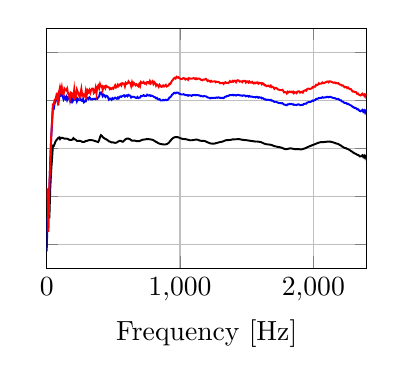
\begin{tikzpicture}

\begin{axis}[%
width=1.6in,
height=1.2in,
at={(1.011in,0.642in)},
scale only axis,
xmin=0,
xmax=2400,
xmajorgrids,
ymin=-30,
ymax=70,
ymajorgrids,
yticklabels={\empty},
xlabel={Frequency [Hz]},
axis background/.style={fill=white},
legend style={legend cell align=left,align=left,draw=white!15!black}
]
\addplot [color=black,solid,line width=0.7pt]
  table[row sep=crcr]{%
0	-7.06319138244352\\
6.66944096884746	-12.1451580312815\\
13.3388819376949	3.16038127446593\\
20.0083229065424	-9.20169992384766\\
26.6777638753898	2.99231449025392\\
33.3472048442373	10.4267536619528\\
40.0166458130848	15.3999184470329\\
46.6860867819322	21.0446548063046\\
53.3555277507797	20.9348892341851\\
60.0249687196271	21.8708533669927\\
66.6944096884746	22.8518234506085\\
73.363850657322	23.3578792470604\\
80.0332916261695	23.8315096670983\\
86.702732595017	24.3089943017668\\
93.3721735638644	24.5063679281205\\
100.041614532712	23.8322664031605\\
106.711055501559	24.3448985900992\\
113.380496470407	24.2763731563769\\
120.049937439254	24.2753569302173\\
126.719378408102	24.1446764899339\\
133.388819376949	23.9878327816752\\
140.058260345797	23.9638239359001\\
146.727701314644	23.9835990674547\\
153.397142283492	23.936499491716\\
160.066583252339	23.8538335978623\\
166.736024221186	23.5865641726001\\
173.405465190034	23.4807777991426\\
180.074906158881	23.4105302027429\\
186.744347127729	23.5131436267766\\
193.413788096576	23.5589188939945\\
200.083229065424	24.1742597778778\\
206.752670034271	23.8071383161221\\
213.422111003119	23.6906719549896\\
220.091551971966	23.3936046288611\\
226.760992940814	23.0786264423957\\
233.430433909661	22.9944680696515\\
240.099874878509	23.0781701951232\\
246.769315847356	23.064198357722\\
253.438756816203	22.9962026800357\\
260.108197785051	22.8479502262225\\
266.777638753898	22.6678448981319\\
273.447079722746	22.6055554645273\\
280.116520691593	22.6052864894416\\
286.785961660441	22.8138448272557\\
293.455402629288	23.0306327303606\\
300.124843598136	23.0038864034444\\
306.794284566983	23.2065895931334\\
313.463725535831	23.2890059433699\\
320.133166504678	23.4256534755755\\
326.802607473525	23.3792231512437\\
333.472048442373	23.3911741853012\\
340.14148941122	23.3388760517908\\
346.810930380068	23.2854804660844\\
353.480371348915	23.1615036477575\\
360.149812317763	23.0588420718461\\
366.81925328661	22.9484156683301\\
373.488694255458	22.7910986888629\\
380.158135224305	22.6705867866769\\
386.827576193153	22.5872809239573\\
393.497017162	23.3523271677458\\
400.166458130848	24.6535374824678\\
406.835899099695	25.4270801667516\\
413.505340068542	25.1578200000981\\
420.17478103739	24.6472874907869\\
426.844222006237	24.3136581657208\\
433.513662975085	24.1279495095204\\
440.183103943932	23.8717623904963\\
446.85254491278	23.7119199095775\\
453.521985881627	23.4920947661414\\
460.191426850475	23.2266876430143\\
466.860867819322	22.8931818998201\\
473.53030878817	22.7581671537331\\
480.199749757017	22.6038907247508\\
486.869190725864	22.4334934651164\\
493.538631694712	22.4505367781308\\
500.208072663559	22.4247202529911\\
506.877513632407	22.3066933046325\\
513.546954601254	22.2371291158751\\
520.216395570102	22.3009587251478\\
526.885836538949	22.4268696961867\\
533.555277507797	22.7009195131517\\
540.224718476644	22.8939308167344\\
546.894159445492	23.0558479826009\\
553.563600414339	23.1153451817359\\
560.233041383186	22.9619362228825\\
566.902482352034	22.694653102095\\
573.571923320881	22.7593739906704\\
580.241364289729	23.1871219906923\\
586.910805258576	23.5293169495787\\
593.580246227424	23.8093649713679\\
600.249687196271	23.974510355603\\
606.919128165119	23.9980303940092\\
613.588569133966	23.9914576322375\\
620.258010102814	23.870813682602\\
626.927451071661	23.6485757989889\\
633.596892040508	23.3509515392212\\
640.266333009356	23.1218111378815\\
646.935773978203	23.1311766989657\\
653.605214947051	23.2063352304861\\
660.274655915898	23.1796183980139\\
666.944096884746	23.0795662676888\\
673.613537853593	22.9810324444067\\
680.282978822441	22.9504721391357\\
686.952419791288	22.8989721282016\\
693.621860760136	22.9620591638546\\
700.291301728983	23.0966701833525\\
706.960742697831	23.2734076243887\\
713.630183666678	23.4174902741207\\
720.299624635525	23.5362964537759\\
726.969065604373	23.6078362871932\\
733.63850657322	23.6397579093734\\
740.307947542068	23.6902258181344\\
746.977388510915	23.7607004229307\\
753.646829479763	23.8293388499664\\
760.31627044861	23.8203939893834\\
766.985711417458	23.7566351488287\\
773.655152386305	23.7191068693044\\
780.324593355153	23.6591892835641\\
786.994034324	23.600879219085\\
793.663475292847	23.5147422661563\\
800.332916261695	23.335942241924\\
807.002357230542	23.1126185748061\\
813.67179819939	22.8690361822297\\
820.341239168237	22.6535730969385\\
827.010680137085	22.4871204509779\\
833.680121105932	22.2201635955721\\
840.34956207478	22.0333884830502\\
847.019003043627	21.9075415763448\\
853.688444012475	21.7895520880448\\
860.357884981322	21.7273065170365\\
867.02732595017	21.6548872501727\\
873.696766919017	21.6126899742938\\
880.366207887864	21.5518558062479\\
887.035648856712	21.5597808054118\\
893.705089825559	21.6332341222736\\
900.374530794407	21.7101546138927\\
907.043971763254	21.9000910623497\\
913.713412732102	22.1993017782688\\
920.382853700949	22.5991181864165\\
927.052294669797	23.028016019812\\
933.721735638644	23.467367720799\\
940.391176607492	23.8632377382619\\
947.060617576339	24.1960281232587\\
953.730058545186	24.4407227970386\\
960.399499514034	24.5675555226621\\
967.068940482881	24.6194509316548\\
973.738381451729	24.6490580820202\\
980.407822420576	24.6393857278688\\
987.077263389424	24.5385022062083\\
993.746704358271	24.401408206066\\
1000.41614532712	24.2489539259459\\
1007.08558629597	24.0882536255018\\
1013.75502726481	23.976556252966\\
1020.42446823366	23.8755563893749\\
1027.09390920251	23.8353310831343\\
1033.76335017136	23.7909556914812\\
1040.4327911402	23.769710657858\\
1047.10223210905	23.734552173249\\
1053.7716730779	23.6233251690137\\
1060.44111404675	23.4985308670891\\
1067.11055501559	23.4339479658537\\
1073.77999598444	23.3383755945164\\
1080.44943695329	23.3095911386122\\
1087.11887792214	23.3207462780992\\
1093.78831889098	23.3695384741972\\
1100.45775985983	23.4189255975373\\
1107.12720082868	23.5101952543536\\
1113.79664179753	23.5635053076485\\
1120.46608276637	23.6037772383247\\
1127.13552373522	23.5918770897338\\
1133.80496470407	23.5190554593735\\
1140.47440567292	23.3537392985243\\
1147.14384664176	23.2352018405017\\
1153.81328761061	23.1072834289739\\
1160.48272857946	23.0938070517795\\
1167.15216954831	23.0716663015272\\
1173.82161051715	23.0432825117372\\
1180.491051486	23.0657111179842\\
1187.16049245485	22.9741364739857\\
1193.82993342369	22.8137558041579\\
1200.49937439254	22.6250012320161\\
1207.16881536139	22.4505511086053\\
1213.83825633024	22.3113645644702\\
1220.50769729908	22.164409486473\\
1227.17713826793	22.0082999928813\\
1233.84657923678	21.9676609515433\\
1240.51602020563	21.9231528205977\\
1247.18546117447	21.8958625057574\\
1253.85490214332	21.9280384152019\\
1260.52434311217	21.9692605545274\\
1267.19378408102	22.0525534894168\\
1273.86322504986	22.1759828633459\\
1280.53266601871	22.2568473767416\\
1287.20210698756	22.3818305288637\\
1293.87154795641	22.477163964524\\
1300.54098892525	22.5422767803392\\
1307.2104298941	22.6409009677265\\
1313.87987086295	22.709672891519\\
1320.5493118318	22.7993688261483\\
1327.21875280064	22.9347337625163\\
1333.88819376949	23.1443230981857\\
1340.55763473834	23.2604593807613\\
1347.22707570719	23.3399139902112\\
1353.89651667603	23.4254992843556\\
1360.56595764488	23.3891598316664\\
1367.23539861373	23.416889195633\\
1373.90483958258	23.4442121543705\\
1380.57428055142	23.5052627479317\\
1387.24372152027	23.571490998877\\
1393.91316248912	23.6774055056387\\
1400.58260345797	23.7078977892927\\
1407.25204442681	23.708718295702\\
1413.92148539566	23.7359014039955\\
1420.59092636451	23.7260488187963\\
1427.26036733336	23.753410088324\\
1433.9298083022	23.7905512463666\\
1440.59924927105	23.7738878051738\\
1447.2686902399	23.7526683773588\\
1453.93813120875	23.6959858395099\\
1460.60757217759	23.5872534400716\\
1467.27701314644	23.5227792836842\\
1473.94645411529	23.4709795705199\\
1480.61589508414	23.4454612965588\\
1487.28533605298	23.3963332916565\\
1493.95477702183	23.3670587195179\\
1500.62421799068	23.3287161434353\\
1507.29365895953	23.2877387756694\\
1513.96309992837	23.1980467232678\\
1520.63254089722	23.1699275214922\\
1527.30198186607	23.1008988008545\\
1533.97142283492	23.0537139211673\\
1540.64086380376	22.9886680834517\\
1547.31030477261	22.9486774888232\\
1553.97974574146	22.8650323280442\\
1560.64918671031	22.8309797380963\\
1567.31862767915	22.7751693262918\\
1573.988068648	22.8090355668654\\
1580.65750961685	22.7787235516967\\
1587.32695058569	22.7203632674655\\
1593.99639155454	22.6895199736348\\
1600.66583252339	22.6276817752039\\
1607.33527349224	22.5273542919189\\
1614.00471446108	22.3566411016534\\
1620.67415542993	22.2154629303636\\
1627.34359639878	22.0317709205555\\
1634.01303736763	21.8621473441639\\
1640.68247833647	21.7625423672946\\
1647.35191930532	21.6654700057895\\
1654.02136027417	21.6336379291417\\
1660.69080124302	21.5862514851679\\
1667.36024221186	21.5309799764266\\
1674.02968318071	21.4748824943473\\
1680.69912414956	21.4480788483643\\
1687.36856511841	21.3202231436708\\
1694.03800608725	21.1903550862246\\
1700.7074470561	21.0327264352085\\
1707.37688802495	20.868773305742\\
1714.0463289938	20.7938857291816\\
1720.71576996264	20.7072669892485\\
1727.38521093149	20.6235794444098\\
1734.05465190034	20.5497614168327\\
1740.72409286919	20.484194511207\\
1747.39353383803	20.4282404919774\\
1754.06297480688	20.3519227013569\\
1760.73241577573	20.2137507238865\\
1767.40185674458	20.1123763962714\\
1774.07129771342	19.9373284354057\\
1780.74073868227	19.7644216293502\\
1787.41017965112	19.6825290766704\\
1794.07962061997	19.6248981538527\\
1800.74906158881	19.6272568348447\\
1807.41850255766	19.7200743949889\\
1814.08794352651	19.7904410940834\\
1820.75738449536	19.9040430353901\\
1827.4268254642	19.9249963700176\\
1834.09626643305	19.9112925570905\\
1840.7657074019	19.8445480699419\\
1847.43514837075	19.7661904155668\\
1854.10458933959	19.7101002608122\\
1860.77403030844	19.6174893657689\\
1867.44347127729	19.6017719659711\\
1874.11291224614	19.6177786482617\\
1880.78235321498	19.6402144552531\\
1887.45179418383	19.6221827413986\\
1894.12123515268	19.5986367809\\
1900.79067612153	19.5393518654393\\
1907.46011709037	19.5175051943906\\
1914.12955805922	19.5670643415398\\
1920.79899902807	19.6459851158212\\
1927.46843999692	19.7867400933474\\
1934.13788096576	19.8926904751843\\
1940.80732193461	20.0424518402586\\
1947.47676290346	20.1847556190499\\
1954.14620387231	20.4073892148293\\
1960.81564484115	20.5397063334415\\
1967.48508581	20.7018477271608\\
1974.15452677885	20.8872794555589\\
1980.82396774769	20.9958073465021\\
1987.49340871654	21.1859349107484\\
1994.16284968539	21.3176185696986\\
2000.83229065424	21.4466123119709\\
2007.50173162308	21.5920780613251\\
2014.17117259193	21.7354898063104\\
2020.84061356078	21.9079170164428\\
2027.51005452963	22.0619367659531\\
2034.17949549847	22.1871249114343\\
2040.84893646732	22.3237882242896\\
2047.51837743617	22.4158067908565\\
2054.18781840502	22.5203484390285\\
2060.85725937386	22.5219531727158\\
2067.52670034271	22.5825494881397\\
2074.19614131156	22.5666109091237\\
2080.86558228041	22.5914760992158\\
2087.53502324925	22.6208798203079\\
2094.2044642181	22.6574102647639\\
2100.87390518695	22.7149503837423\\
2107.5433461558	22.7692877418663\\
2114.21278712464	22.7436452274783\\
2120.88222809349	22.8037805070618\\
2127.55166906234	22.7496510286228\\
2134.22111003119	22.6384629954685\\
2140.89055100003	22.5436634497396\\
2147.55999196888	22.4657952023925\\
2154.22943293773	22.3111319774926\\
2160.89887390658	22.2571980563019\\
2167.56831487542	22.0534596905007\\
2174.23775584427	21.9615628146826\\
2180.90719681312	21.8610889619323\\
2187.57663778197	21.7384083474387\\
2194.24607875081	21.4905122820051\\
2200.91551971966	21.2724296073177\\
2207.58496068851	21.1046994458229\\
2214.25440165736	20.7515462427339\\
2220.9238426262	20.5899673172011\\
2227.59328359505	20.2955811191359\\
2234.2627245639	20.1392277600802\\
2240.93216553275	20.06929755624\\
2247.60160650159	19.9640351948554\\
2254.27104747044	19.6912274824231\\
2260.94048843929	19.5768979053963\\
2267.60992940814	19.4142115723179\\
2274.27937037698	19.1524169275647\\
2280.94881134583	18.895551532986\\
2287.61825231468	18.7012224211693\\
2294.28769328353	18.3911049790877\\
2300.95713425237	18.1592446996668\\
2307.62657522122	17.8694643161592\\
2314.29601619007	17.7777007237746\\
2320.96545715892	17.5816589800523\\
2327.63489812776	17.2755214115182\\
2334.30433909661	17.2239077028895\\
2340.97378006546	17.0252785399023\\
2347.64322103431	16.5943194755682\\
2354.31266200315	16.5783416984111\\
2360.982102972	16.758377289574\\
2367.65154394085	17.0667399116852\\
2374.3209849097	16.3535263704576\\
2380.99042587854	16.8795126905889\\
2387.65986684739	16.0390068540478\\
2394.32930781624	17.2527685157111\\
};

\addplot [color=blue,solid,line width=0.7pt]
  table[row sep=crcr]{%
0	-22.954064049475\\
6.66944096884746	-9.78857180415678\\
13.3388819376949	-6.77059814713491\\
20.0083229065424	2.14620695077614\\
26.6777638753898	14.1256052273745\\
33.3472048442373	23.5821369780091\\
40.0166458130848	30.339360790699\\
46.6860867819322	36.7576510797684\\
53.3555277507797	36.4977460750246\\
60.0249687196271	38.7813087349974\\
66.6944096884746	39.4493428692619\\
73.363850657322	40.7934899110689\\
80.0332916261695	41.1881632898965\\
86.702732595017	42.5827543367591\\
93.3721735638644	40.9891982644943\\
100.041614532712	43.2561471319915\\
106.711055501559	41.9335624937319\\
113.380496470407	42.1915238630746\\
120.049937439254	41.6388114771807\\
126.719378408102	40.3983677150193\\
133.388819376949	41.2762163035143\\
140.058260345797	40.5942071360353\\
146.727701314644	41.4326380320027\\
153.397142283492	40.1173741458733\\
160.066583252339	41.0898196189013\\
166.736024221186	40.6741178042262\\
173.405465190034	40.1176293179382\\
180.074906158881	39.5143038322728\\
186.744347127729	40.9106668219849\\
193.413788096576	39.443237356967\\
200.083229065424	39.9972353592753\\
206.752670034271	41.2959132763171\\
213.422111003119	40.4937548384365\\
220.091551971966	41.2281031983082\\
226.760992940814	39.5754321124854\\
233.430433909661	40.5503903510572\\
240.099874878509	40.063868284513\\
246.769315847356	40.0234221432809\\
253.438756816203	40.5165474806229\\
260.108197785051	39.8889284314908\\
266.777638753898	39.7020987891783\\
273.447079722746	40.5421924304781\\
280.116520691593	39.1321590528798\\
286.785961660441	39.5000705897022\\
293.455402629288	39.5263072686429\\
300.124843598136	41.1177838546136\\
306.794284566983	40.886513454779\\
313.463725535831	40.4857082011309\\
320.133166504678	41.1638958925782\\
326.802607473525	40.7891923847122\\
333.472048442373	40.2982038903473\\
340.14148941122	40.2873425269961\\
346.810930380068	40.5354842167478\\
353.480371348915	40.5303067226592\\
360.149812317763	40.6157198212441\\
366.81925328661	40.4108892218855\\
373.488694255458	40.8505458922836\\
380.158135224305	40.6360078102458\\
386.827576193153	41.2538014839218\\
393.497017162	41.5532281273484\\
400.166458130848	43.1276125452504\\
406.835899099695	43.2691455809521\\
413.505340068542	42.6701584413612\\
420.17478103739	41.6927541858549\\
426.844222006237	42.3094868182956\\
433.513662975085	41.9912053920141\\
440.183103943932	41.362452285189\\
446.85254491278	41.8753570308684\\
453.521985881627	41.7331236901833\\
460.191426850475	41.1737579257221\\
466.860867819322	40.256986130489\\
473.53030878817	40.6690009768915\\
480.199749757017	40.652877600612\\
486.869190725864	40.1969768816923\\
493.538631694712	40.8400495475925\\
500.208072663559	40.5353728833734\\
506.877513632407	40.7311869011286\\
513.546954601254	41.0660962655341\\
520.216395570102	40.8093342485518\\
526.885836538949	40.6010501613812\\
533.555277507797	41.108719080586\\
540.224718476644	40.7672798321522\\
546.894159445492	41.4514314940318\\
553.563600414339	41.5929842821907\\
560.233041383186	41.3841515907344\\
566.902482352034	41.8053764362042\\
573.571923320881	41.856383326638\\
580.241364289729	42.0572286811247\\
586.910805258576	41.5311173540256\\
593.580246227424	41.913802833506\\
600.249687196271	42.0511631962903\\
606.919128165119	41.6629960043171\\
613.588569133966	42.2074295631877\\
620.258010102814	42.0092226730831\\
626.927451071661	41.8854896371517\\
633.596892040508	41.1426471099475\\
640.266333009356	41.3961384487332\\
646.935773978203	41.4653785338685\\
653.605214947051	41.4464449289932\\
660.274655915898	41.2557611565269\\
666.944096884746	41.0367405596191\\
673.613537853593	40.9342498673582\\
680.282978822441	41.3504480947361\\
686.952419791288	40.8994297505606\\
693.621860760136	41.0810461727534\\
700.291301728983	41.1184506067919\\
706.960742697831	41.7734268034009\\
713.630183666678	41.6936369012161\\
720.299624635525	41.8386045488136\\
726.969065604373	42.1092619623957\\
733.63850657322	41.7442777638835\\
740.307947542068	41.8007500299447\\
746.977388510915	41.8337900782482\\
753.646829479763	42.3032142093445\\
760.31627044861	42.0323044649073\\
766.985711417458	41.9361438722392\\
773.655152386305	42.1453597937723\\
780.324593355153	41.7722999102125\\
786.994034324	41.9211993329326\\
793.663475292847	41.7515258428662\\
800.332916261695	41.574030820325\\
807.002357230542	41.3319258752026\\
813.67179819939	41.2276835130635\\
820.341239168237	40.7873178667278\\
827.010680137085	40.9535341880206\\
833.680121105932	40.4590097801008\\
840.34956207478	40.2976102268526\\
847.019003043627	40.4534820006419\\
853.688444012475	39.9557499198277\\
860.357884981322	39.882470279775\\
867.02732595017	39.8852692471632\\
873.696766919017	40.1632688196347\\
880.366207887864	39.9690843455612\\
887.035648856712	40.0326793797131\\
893.705089825559	40.2123840061145\\
900.374530794407	40.0143928700985\\
907.043971763254	40.1518850722719\\
913.713412732102	40.4676569130535\\
920.382853700949	41.1480333410688\\
927.052294669797	41.2412380056518\\
933.721735638644	41.6890430166831\\
940.391176607492	42.3069500040496\\
947.060617576339	42.5640879038934\\
953.730058545186	42.9940117938683\\
960.399499514034	43.1116302409091\\
967.068940482881	42.8960011932377\\
973.738381451729	43.2104439827877\\
980.407822420576	43.2074541434081\\
987.077263389424	43.0678542279588\\
993.746704358271	42.7405729377433\\
1000.41614532712	42.6151215510219\\
1007.08558629597	42.4483774123285\\
1013.75502726481	42.3744194019021\\
1020.42446823366	42.3832063032982\\
1027.09390920251	42.5194561266286\\
1033.76335017136	42.3107805010744\\
1040.4327911402	42.1444938337345\\
1047.10223210905	42.1547190423105\\
1053.7716730779	42.1135023836828\\
1060.44111404675	41.8769013333215\\
1067.11055501559	42.1191169865354\\
1073.77999598444	42.0327992571925\\
1080.44943695329	42.0461956383478\\
1087.11887792214	41.8190941628667\\
1093.78831889098	42.1029873586186\\
1100.45775985983	42.1544383881245\\
1107.12720082868	42.2220415086041\\
1113.79664179753	42.0659785795335\\
1120.46608276637	42.1892370616687\\
1127.13552373522	42.1386422880497\\
1133.80496470407	42.1327560222299\\
1140.47440567292	42.0036472582347\\
1147.14384664176	41.9835354128199\\
1153.81328761061	41.7329058580801\\
1160.48272857946	41.7810216010089\\
1167.15216954831	41.5953911716803\\
1173.82161051715	41.6059638967908\\
1180.491051486	41.7799746822254\\
1187.16049245485	41.6445425865687\\
1193.82993342369	41.6535018493812\\
1200.49937439254	41.4044091680929\\
1207.16881536139	41.1716837875984\\
1213.83825633024	41.0686938160251\\
1220.50769729908	41.0018490152226\\
1227.17713826793	40.782254480469\\
1233.84657923678	40.996662816826\\
1240.51602020563	40.9133091321949\\
1247.18546117447	40.9799980166256\\
1253.85490214332	40.9970744230188\\
1260.52434311217	41.0303202178618\\
1267.19378408102	40.9977295112348\\
1273.86322504986	41.154194242003\\
1280.53266601871	41.0186216706051\\
1287.20210698756	41.1757668873816\\
1293.87154795641	41.1280127202126\\
1300.54098892525	40.9055561941224\\
1307.2104298941	41.0350238876599\\
1313.87987086295	40.9659604546095\\
1320.5493118318	40.992475685865\\
1327.21875280064	40.882164027574\\
1333.88819376949	41.2482767608877\\
1340.55763473834	41.5039633858864\\
1347.22707570719	41.5168725126964\\
1353.89651667603	41.7868512478219\\
1360.56595764488	41.7753022355428\\
1367.23539861373	41.9299307798422\\
1373.90483958258	42.1802277005252\\
1380.57428055142	42.154005829488\\
1387.24372152027	42.117815771325\\
1393.91316248912	42.2568145939493\\
1400.58260345797	42.0264606516659\\
1407.25204442681	42.205729224344\\
1413.92148539566	42.1361782959898\\
1420.59092636451	41.9540414329128\\
1427.26036733336	42.1710722396394\\
1433.9298083022	42.2789371368837\\
1440.59924927105	42.1811334544795\\
1447.2686902399	42.0393429848363\\
1453.93813120875	42.0357916138406\\
1460.60757217759	41.9160386866317\\
1467.27701314644	41.8517675484475\\
1473.94645411529	41.9988688341219\\
1480.61589508414	41.9887770084685\\
1487.28533605298	41.9233066419397\\
1493.95477702183	41.6317358303567\\
1500.62421799068	41.8535246979039\\
1507.29365895953	41.8484136780946\\
1513.96309992837	41.5229368775499\\
1520.63254089722	41.7642348111048\\
1527.30198186607	41.5250124417307\\
1533.97142283492	41.451338649284\\
1540.64086380376	41.5333337446132\\
1547.31030477261	41.3266372679848\\
1553.97974574146	41.246812872336\\
1560.64918671031	41.359210003823\\
1567.31862767915	41.1548676023768\\
1573.988068648	41.3945635994426\\
1580.65750961685	41.3642743723405\\
1587.32695058569	41.0259376168935\\
1593.99639155454	41.2612856737108\\
1600.66583252339	41.101769216229\\
1607.33527349224	41.1420557230952\\
1614.00471446108	40.7402374758875\\
1620.67415542993	40.876550048051\\
1627.34359639878	40.6836131597097\\
1634.01303736763	40.3333217111692\\
1640.68247833647	40.3974519843421\\
1647.35191930532	40.1181591955561\\
1654.02136027417	40.1839297941091\\
1660.69080124302	40.2418780553085\\
1667.36024221186	40.1157826999337\\
1674.02968318071	39.9907589092101\\
1680.69912414956	40.1662124769885\\
1687.36856511841	39.7758038032028\\
1694.03800608725	39.8001407724914\\
1700.7074470561	39.6243542124833\\
1707.37688802495	39.2858110963831\\
1714.0463289938	39.3721544451289\\
1720.71576996264	39.3495671947385\\
1727.38521093149	39.1610641899692\\
1734.05465190034	38.9964032395012\\
1740.72409286919	38.8724266193129\\
1747.39353383803	38.8104957511629\\
1754.06297480688	38.7949070333307\\
1760.73241577573	38.709052880172\\
1767.40185674458	38.7890224674643\\
1774.07129771342	38.4824048294331\\
1780.74073868227	38.1776787430737\\
1787.41017965112	38.1037170783283\\
1794.07962061997	38.0753516245127\\
1800.74906158881	37.9335247277797\\
1807.41850255766	38.2812432484186\\
1814.08794352651	38.255991005054\\
1820.75738449536	38.4970894328548\\
1827.4268254642	38.3895570411657\\
1834.09626643305	38.4964891795799\\
1840.7657074019	38.2973193158254\\
1847.43514837075	38.3355260435024\\
1854.10458933959	38.0237283768604\\
1860.77403030844	38.1279872487974\\
1867.44347127729	38.0855859786085\\
1874.11291224614	37.9850910992675\\
1880.78235321498	38.2214860185808\\
1887.45179418383	38.2903828101694\\
1894.12123515268	38.2025820085478\\
1900.79067612153	37.9391552314051\\
1907.46011709037	37.9802873699483\\
1914.12955805922	38.0906760741873\\
1920.79899902807	38.0237686621922\\
1927.46843999692	38.3797060720391\\
1934.13788096576	38.4601687383869\\
1940.80732193461	38.6271721702318\\
1947.47676290346	38.6116573183312\\
1954.14620387231	39.0243765712576\\
1960.81564484115	39.1617304228675\\
1967.48508581	39.2093807626978\\
1974.15452677885	39.2762109995117\\
1980.82396774769	39.3585831820616\\
1987.49340871654	39.5366273167703\\
1994.16284968539	39.875703369154\\
2000.83229065424	39.7581105148084\\
2007.50173162308	39.9957643118495\\
2014.17117259193	40.0718964499888\\
2020.84061356078	40.5295960626087\\
2027.51005452963	40.5397161483685\\
2034.17949549847	40.6414219209252\\
2040.84893646732	40.9680598492434\\
2047.51837743617	40.858524850133\\
2054.18781840502	41.0083983807823\\
2060.85725937386	40.9860195800659\\
2067.52670034271	41.2466919218044\\
2074.19614131156	41.0446215119225\\
2080.86558228041	41.0934742410651\\
2087.53502324925	41.2315478785773\\
2094.2044642181	41.1993403213241\\
2100.87390518695	41.4005543212765\\
2107.5433461558	41.4086340747035\\
2114.21278712464	41.2238015063502\\
2120.88222809349	41.4249278526462\\
2127.55166906234	41.4384068645908\\
2134.22111003119	41.2257888262826\\
2140.89055100003	41.150267729775\\
2147.55999196888	41.0031629141457\\
2154.22943293773	40.8631200671276\\
2160.89887390658	40.9257972232752\\
2167.56831487542	40.6231335915654\\
2174.23775584427	40.5911330657136\\
2180.90719681312	40.5008391538439\\
2187.57663778197	40.5353377427996\\
2194.24607875081	40.1818097911681\\
2200.91551971966	39.9904587046543\\
2207.58496068851	39.9501394754442\\
2214.25440165736	39.498802447519\\
2220.9238426262	39.4424602021105\\
2227.59328359505	39.0930917058234\\
2234.2627245639	38.9105472992056\\
2240.93216553275	38.8100989841084\\
2247.60160650159	38.7741102216817\\
2254.27104747044	38.3990945260412\\
2260.94048843929	38.4677013870502\\
2267.60992940814	38.2594469704934\\
2274.27937037698	38.0240558397041\\
2280.94881134583	37.8390430290234\\
2287.61825231468	37.6348872222803\\
2294.28769328353	37.2812261884329\\
2300.95713425237	37.1421029600459\\
2307.62657522122	36.8402936340167\\
2314.29601619007	36.8188057531817\\
2320.96545715892	36.6470270596275\\
2327.63489812776	36.1952261845239\\
2334.30433909661	36.2604829582675\\
2340.97378006546	35.9171465776459\\
2347.64322103431	35.5476474852302\\
2354.31266200315	35.3928228651849\\
2360.982102972	35.6884041135166\\
2367.65154394085	35.9747648675445\\
2374.3209849097	35.1810454294486\\
2380.99042587854	35.7025895532202\\
2387.65986684739	34.8704261909491\\
2394.32930781624	36.1174565741079\\
};

\addplot [color=red,solid,line width=0.7pt]
  table[row sep=crcr]{%
0	-0.848881145937375\\
6.66944096884746	3.19945445302707\\
13.3388819376949	-14.8892946472187\\
20.0083229065424	4.39374385344356\\
26.6777638753898	13.3642776124857\\
33.3472048442373	24.0453104228001\\
40.0166458130848	31.1857587224763\\
46.6860867819322	38.2627688228372\\
53.3555277507797	38.3372834849038\\
60.0249687196271	40.1803473894589\\
66.6944096884746	40.4787596888213\\
73.363850657322	42.1503430485016\\
80.0332916261695	41.3229046157928\\
86.702732595017	37.7630703574815\\
93.3721735638644	43.4988290270033\\
100.041614532712	45.4086163930557\\
106.711055501559	43.5689593033832\\
113.380496470407	45.3705462973518\\
120.049937439254	42.8098213381692\\
126.719378408102	42.3566866825008\\
133.388819376949	44.8093452559768\\
140.058260345797	44.2928233766816\\
146.727701314644	44.0563663951681\\
153.397142283492	44.8477110186835\\
160.066583252339	42.8042501000734\\
166.736024221186	42.3640612124917\\
173.405465190034	40.3303355606033\\
180.074906158881	43.2008748647143\\
186.744347127729	42.9708102696148\\
193.413788096576	41.6196511972445\\
200.083229065424	41.162148424414\\
206.752670034271	44.4308449625708\\
213.422111003119	40.8437562656049\\
220.091551971966	41.2223106752822\\
226.760992940814	44.3724835529836\\
233.430433909661	43.4014993706388\\
240.099874878509	42.7188259797762\\
246.769315847356	41.2247772722969\\
253.438756816203	42.4697654898201\\
260.108197785051	44.6800092411187\\
266.777638753898	41.907617836434\\
273.447079722746	42.5082020531911\\
280.116520691593	42.0338623019318\\
286.785961660441	41.5718855742805\\
293.455402629288	43.9258914496967\\
300.124843598136	42.0778756103412\\
306.794284566983	44.0547478362224\\
313.463725535831	43.4133994496596\\
320.133166504678	44.2378038696381\\
326.802607473525	43.0056788191629\\
333.472048442373	44.267382875656\\
340.14148941122	44.8324561015541\\
346.810930380068	44.8635684160498\\
353.480371348915	42.9880951486122\\
360.149812317763	43.4292113874217\\
366.81925328661	45.1092080765489\\
373.488694255458	42.8292903347091\\
380.158135224305	45.5633792722838\\
386.827576193153	46.1309307973711\\
393.497017162	44.978865302705\\
400.166458130848	46.7307269635864\\
406.835899099695	45.7912456047856\\
413.505340068542	45.9522975141447\\
420.17478103739	44.3307312055842\\
426.844222006237	45.7673598902482\\
433.513662975085	45.8168471292992\\
440.183103943932	44.9842728606719\\
446.85254491278	45.9853062885995\\
453.521985881627	45.656258229778\\
460.191426850475	45.4186123921121\\
466.860867819322	45.3723890288207\\
473.53030878817	44.614489820492\\
480.199749757017	44.9434991797149\\
486.869190725864	44.684427582117\\
493.538631694712	45.1463641368097\\
500.208072663559	44.8370034626217\\
506.877513632407	45.4594468294472\\
513.546954601254	46.2105559415203\\
520.216395570102	45.273272719683\\
526.885836538949	45.5659827337093\\
533.555277507797	46.4694288556552\\
540.224718476644	45.9112344320299\\
546.894159445492	46.4905963112887\\
553.563600414339	46.7579032160724\\
560.233041383186	46.1470393489715\\
566.902482352034	47.1218583663798\\
573.571923320881	46.9260702561973\\
580.241364289729	46.946796266769\\
586.910805258576	45.7660792034303\\
593.580246227424	47.2419756565228\\
600.249687196271	46.845917314362\\
606.919128165119	47.0058078094769\\
613.588569133966	47.8289023165749\\
620.258010102814	47.278126105846\\
626.927451071661	47.1977513526711\\
633.596892040508	45.9146611308723\\
640.266333009356	47.5037629009485\\
646.935773978203	46.3990845961037\\
653.605214947051	47.219105250547\\
660.274655915898	46.7414774361541\\
666.944096884746	46.2302127929431\\
673.613537853593	46.6334235979056\\
680.282978822441	46.2249923099107\\
686.952419791288	45.8091669694066\\
693.621860760136	46.7236297334056\\
700.291301728983	45.8544672149714\\
706.960742697831	47.5706352708832\\
713.630183666678	47.2135948253799\\
720.299624635525	47.2369974661712\\
726.969065604373	47.6203164154259\\
733.63850657322	46.9444656894577\\
740.307947542068	47.145084581688\\
746.977388510915	46.7839855949191\\
753.646829479763	47.6258848471732\\
760.31627044861	47.532798755161\\
766.985711417458	47.1448219719876\\
773.655152386305	47.9940957810839\\
780.324593355153	46.9903999753267\\
786.994034324	47.435966670887\\
793.663475292847	47.8935564124965\\
800.332916261695	46.8059247481705\\
807.002357230542	47.5397157946341\\
813.67179819939	47.1045452672334\\
820.341239168237	46.0117611832548\\
827.010680137085	46.5624339551265\\
833.680121105932	46.2609839473673\\
840.34956207478	45.5776552622929\\
847.019003043627	46.4374272715314\\
853.688444012475	46.0156078031355\\
860.357884981322	45.5650247141215\\
867.02732595017	45.6817068234894\\
873.696766919017	46.1628361926261\\
880.366207887864	45.7238473741303\\
887.035648856712	46.0934756962619\\
893.705089825559	46.4003461063302\\
900.374530794407	45.7556888744374\\
907.043971763254	46.0054018147989\\
913.713412732102	46.087829676541\\
920.382853700949	46.8762319341298\\
927.052294669797	46.7624888967295\\
933.721735638644	47.460517154299\\
940.391176607492	48.1408490609948\\
947.060617576339	48.4759159381572\\
953.730058545186	49.1314152495934\\
960.399499514034	49.3259032477091\\
967.068940482881	49.0170423549744\\
973.738381451729	49.767099694053\\
980.407822420576	49.4557174547624\\
987.077263389424	49.6031093167001\\
993.746704358271	49.1902059586768\\
1000.41614532712	49.0625935756709\\
1007.08558629597	48.8078226279566\\
1013.75502726481	48.8393873878442\\
1020.42446823366	49.0945024243369\\
1027.09390920251	49.1981780431319\\
1033.76335017136	49.1070752163037\\
1040.4327911402	48.6116577919909\\
1047.10223210905	48.8533496855164\\
1053.7716730779	48.9894466719249\\
1060.44111404675	48.5185720521716\\
1067.11055501559	49.2077741376971\\
1073.77999598444	49.0016819122943\\
1080.44943695329	49.0428951386214\\
1087.11887792214	48.9735223741657\\
1093.78831889098	49.0541470413033\\
1100.45775985983	49.180441653277\\
1107.12720082868	49.1664110888982\\
1113.79664179753	48.8253274511295\\
1120.46608276637	49.1506995170164\\
1127.13552373522	48.7967091868681\\
1133.80496470407	48.966131314861\\
1140.47440567292	49.0033585732632\\
1147.14384664176	49.0252018844559\\
1153.81328761061	48.6032500199771\\
1160.48272857946	48.4502029228781\\
1167.15216954831	48.3107961215402\\
1173.82161051715	48.6129116953796\\
1180.491051486	48.5669148093087\\
1187.16049245485	48.6454761510052\\
1193.82993342369	48.9302454487942\\
1200.49937439254	48.5151577603833\\
1207.16881536139	47.975900974454\\
1213.83825633024	48.2346303997164\\
1220.50769729908	48.0432319786956\\
1227.17713826793	47.6836392373022\\
1233.84657923678	48.0713587456892\\
1240.51602020563	47.7232492313724\\
1247.18546117447	47.8182588921118\\
1253.85490214332	47.8086258879778\\
1260.52434311217	47.8926325738321\\
1267.19378408102	47.4844073637142\\
1273.86322504986	47.7206260216287\\
1280.53266601871	47.6143599207396\\
1287.20210698756	47.6853541062759\\
1293.87154795641	47.5082311778596\\
1300.54098892525	47.0718086898822\\
1307.2104298941	47.1496056685904\\
1313.87987086295	47.1029453758342\\
1320.5493118318	47.2474466363965\\
1327.21875280064	46.8003346237001\\
1333.88819376949	47.2319123392215\\
1340.55763473834	47.5166308015754\\
1347.22707570719	47.2487233704463\\
1353.89651667603	47.266283858576\\
1360.56595764488	47.1274901376889\\
1367.23539861373	47.3589909868297\\
1373.90483958258	47.9652151603522\\
1380.57428055142	47.6162385229527\\
1387.24372152027	47.5630306400481\\
1393.91316248912	48.0475221771479\\
1400.58260345797	47.7338439342309\\
1407.25204442681	48.1410869145162\\
1413.92148539566	48.0847643320117\\
1420.59092636451	47.5107713803023\\
1427.26036733336	48.192733649274\\
1433.9298083022	48.3382875637418\\
1440.59924927105	48.1825245008621\\
1447.2686902399	47.7393970613601\\
1453.93813120875	47.8708519093298\\
1460.60757217759	47.8198989556294\\
1467.27701314644	47.5326896796591\\
1473.94645411529	48.098240632994\\
1480.61589508414	48.0534550323788\\
1487.28533605298	48.0780834043454\\
1493.95477702183	47.3748432575166\\
1500.62421799068	47.8956511510947\\
1507.29365895953	47.9033581916132\\
1513.96309992837	47.3575096796836\\
1520.63254089722	47.8423791300717\\
1527.30198186607	47.3799063276748\\
1533.97142283492	47.3062300354595\\
1540.64086380376	47.6646357527883\\
1547.31030477261	47.1897747867321\\
1553.97974574146	46.9701348405767\\
1560.64918671031	47.3095929947923\\
1567.31862767915	47.0657864588131\\
1573.988068648	47.3826831167607\\
1580.65750961685	47.4454102737635\\
1587.32695058569	46.9114832074451\\
1593.99639155454	47.2716447461065\\
1600.66583252339	47.1370347046979\\
1607.33527349224	47.2064108557657\\
1614.00471446108	46.6338718853141\\
1620.67415542993	47.065370340288\\
1627.34359639878	46.769792299551\\
1634.01303736763	46.2414043291666\\
1640.68247833647	46.3288782652738\\
1647.35191930532	45.8502448655545\\
1654.02136027417	45.9428931985082\\
1660.69080124302	46.1154362994239\\
1667.36024221186	45.8584047857448\\
1674.02968318071	45.6512391968312\\
1680.69912414956	46.1058404220061\\
1687.36856511841	45.4458581579309\\
1694.03800608725	45.6163523369514\\
1700.7074470561	45.3812435131459\\
1707.37688802495	44.7610499647815\\
1714.0463289938	45.1559203849385\\
1720.71576996264	45.1294823942954\\
1727.38521093149	44.8732546903864\\
1734.05465190034	44.4938667674189\\
1740.72409286919	44.4287385354572\\
1747.39353383803	44.2647483210354\\
1754.06297480688	44.1685198251547\\
1760.73241577573	44.2712193929554\\
1767.40185674458	44.3631691742058\\
1774.07129771342	43.8998348431296\\
1780.74073868227	43.2577293407314\\
1787.41017965112	43.3545925225926\\
1794.07962061997	43.3356325854545\\
1800.74906158881	42.8073064786482\\
1807.41850255766	43.5553964327627\\
1814.08794352651	43.2615175375231\\
1820.75738449536	43.5862309287241\\
1827.4268254642	43.4719329347032\\
1834.09626643305	43.5777419065745\\
1840.7657074019	43.2723987049217\\
1847.43514837075	43.5772456642628\\
1854.10458933959	42.9220377893572\\
1860.77403030844	43.3555856377472\\
1867.44347127729	43.2967145126314\\
1874.11291224614	42.9369751302581\\
1880.78235321498	43.6302517979804\\
1887.45179418383	43.6813826421235\\
1894.12123515268	43.682083846462\\
1900.79067612153	43.1355217413298\\
1907.46011709037	43.3010399000341\\
1914.12955805922	43.5003298604596\\
1920.79899902807	43.1787712646433\\
1927.46843999692	43.9210373035026\\
1934.13788096576	43.9441432721762\\
1940.80732193461	44.2118062150357\\
1947.47676290346	43.9952348743882\\
1954.14620387231	44.6836185631805\\
1960.81564484115	44.8389001184084\\
1967.48508581	44.8007777704201\\
1974.15452677885	44.6445650540954\\
1980.82396774769	44.820251025219\\
1987.49340871654	44.9305150146499\\
1994.16284968539	45.4992545720069\\
2000.83229065424	45.3557832029697\\
2007.50173162308	45.7176920340627\\
2014.17117259193	45.6533914873725\\
2020.84061356078	46.4484191456078\\
2027.51005452963	46.3371380449344\\
2034.17949549847	46.4482852835538\\
2040.84893646732	47.0617590913164\\
2047.51837743617	46.8101919698897\\
2054.18781840502	46.9737336999286\\
2060.85725937386	46.9560818124684\\
2067.52670034271	47.413014798192\\
2074.19614131156	47.0990479277671\\
2080.86558228041	47.1489010791261\\
2087.53502324925	47.3717549666309\\
2094.2044642181	47.4904041488506\\
2100.87390518695	47.7721336404307\\
2107.5433461558	47.8047656217832\\
2114.21278712464	47.4229170714115\\
2120.88222809349	47.8875692464271\\
2127.55166906234	47.9032877918051\\
2134.22111003119	47.676691120474\\
2140.89055100003	47.5290305140363\\
2147.55999196888	47.3773393195851\\
2154.22943293773	47.268418415075\\
2160.89887390658	47.4267262455074\\
2167.56831487542	47.0941005942479\\
2174.23775584427	47.2159933146185\\
2180.90719681312	46.9855925233881\\
2187.57663778197	47.1006090489495\\
2194.24607875081	46.6481613613665\\
2200.91551971966	46.457046189148\\
2207.58496068851	46.4844207041093\\
2214.25440165736	46.1097272927884\\
2220.9238426262	46.181757571641\\
2227.59328359505	45.8140688399752\\
2234.2627245639	45.39413923896\\
2240.93216553275	45.572050935081\\
2247.60160650159	45.5068347354978\\
2254.27104747044	45.031365223746\\
2260.94048843929	45.2787323488045\\
2267.60992940814	44.841189363904\\
2274.27937037698	44.6560549436405\\
2280.94881134583	44.6616381792946\\
2287.61825231468	44.1798286044703\\
2294.28769328353	43.6461589860504\\
2300.95713425237	43.7220596201554\\
2307.62657522122	43.4183369694571\\
2314.29601619007	43.4555560418186\\
2320.96545715892	43.3397445849421\\
2327.63489812776	42.6989512061204\\
2334.30433909661	42.8048882929911\\
2340.97378006546	42.3085125851336\\
2347.64322103431	42.1341137217499\\
2354.31266200315	41.9861722601077\\
2360.982102972	42.3771787355474\\
2367.65154394085	42.7185235830522\\
2374.3209849097	42.1046003690444\\
2380.99042587854	42.3769817652072\\
2387.65986684739	41.5745275374915\\
2394.32930781624	42.7718513805022\\
};

\end{axis}
\end{tikzpicture}%
	\caption{Microphone tests.}
	\label{fig:freq_responsecomb1}
\end{subfigure}
\caption{Frequency response of (a) the vibration on the driver, (b) the vibration on the enclosure, and (c) the speaker. The black graph is frequency response for dataset 1, the blue for the dataset 10, and the red dataset 19. }
\label{fig:freq_response_comb}
\end{figure}

It can be concluded that the frequency response of between all datasets in each measurement remains almost unchanged, thus it is not possible to derive any indication of the current performance of the loudspeaker. The analysis shows that the gain ratio between the amount of vibration and the sound pressure is linear. Therefore it might be possible to use the accelerometer as a tool to estimate the sound pressure level from the amount of vibration.









